% NOTE: For final SP&E submission, reformat using Wiley's LaTeX template
% (wiley-article class). This draft uses standard article class.
\documentclass[12pt]{article}

\usepackage[margin=1in]{geometry}
\usepackage{booktabs}
\usepackage{subcaption}
\usepackage{xspace}
\usepackage{authblk}
\usepackage{amsmath}
\usepackage{amsthm}
\usepackage{hyperref}
\usepackage{graphicx}
\usepackage{pgfplots}
\usepackage{pdflscape}
\usepackage{longtable}
\pgfplotsset{compat=1.18}

\newcommand{\schubfach}{Schubfach\xspace}
\newcommand{\burgerdybvig}{Burger--Dybvig\xspace}
\newcommand{\ryualg}{Ry\=u\xspace}
\newcommand{\dragonbox}{Dragonbox\xspace}
\newcommand{\ecma}{ECMA-262\xspace}
\newcommand{\rfcjcs}{RFC~8785\xspace}

\theoremstyle{definition}
\newtheorem{definition}{Definition}
\theoremstyle{remark}
\newtheorem{remark}{Remark}

\begin{document}

\title{Fixed-Width vs.\ Multiprecision Digit Generation\\for JSON Canonicalization: A Four-Algorithm Empirical Study}

\author{Mark Lenhardt}
\affil{Lattice Substrate}
\date{}

\maketitle

\begin{abstract}
JSON Canonicalization Scheme (RFC~8785) requires deterministic
floating-point formatting that matches ECMA-262 \texttt{Number::toString}.
We present the first empirical comparison of four digit-generation
algorithms---three fixed-width (\schubfach, \ryualg, \dragonbox) and one
multiprecision (\burgerdybvig)---inside a specification-constrained
canonicalization pipeline, implemented in both Go and Rust
(8~implementations total) to separate algorithmic effects from
language/runtime effects.
Our methodology gates performance measurement on conformance: only
implementations passing 286{,}362 oracle vectors (generated from V8
and validated against SpiderMonkey and JavaScriptCore) and 696
structural conformance cases (87 per
implementation $\times$ 8~implementations) proceed to benchmarking.
Using permutation tests, BCa bootstrap confidence intervals, and
Benjamini--Hochberg FDR correction across 1{,}294 comparisons
(16~pairs $\times$ workloads/modes), we find that all three fixed-width
algorithms perform within 1--8\% of each other across both languages,
while each is 1.4--1.8$\times$ faster than \burgerdybvig on
number-dense workloads ($\nu(D) \geq 40\%$) in Go API benchmarks;
the advantage replicates at 2.3--3.0$\times$ in Rust, confirming it is
algorithmic rather than language-specific (excluding extreme outliers on
\texttt{numeric-boundary} and \texttt{number-heavy} in Rust at
8--9$\times$, discussed in \S\ref{sec:discussion}).
On string-dominant and deeply-nested inputs the difference narrows to
$<$5\%.
All eight implementations produce byte-identical output; Go binaries are
additionally verified under cross-compilation for x86-64 and arm64.
We release the benchmark infrastructure, oracle vectors, and all raw
data as a reproducibility artifact.
\end{abstract}

\noindent\textbf{Keywords:} JSON canonicalization, floating-point formatting, Schubfach,
Ry\=u, Dragonbox, Burger--Dybvig, RFC~8785, ECMA-262, benchmark methodology, cross-language validation

\section{Introduction}
\label{sec:introduction}

The JSON Canonicalization Scheme (\rfcjcs)~\cite{rfc8785} standardizes a
deterministic serialization of JSON values for use in digital signatures,
content-addressable storage, and distributed consensus protocols.  A
critical requirement is that floating-point numbers must be formatted
identically to the output of \ecma \texttt{Number::toString}~\cite{ecma262},
which specifies shortest-representation formatting under roundTiesToEven
semantics.

Several deployment contexts place canonicalization on the critical path.
In high-frequency signature verification, every document must be
canonicalized before its signature can be checked, making formatting
throughput a direct bottleneck.  Content-addressed storage systems hash
the canonical form at both ingestion and retrieval, so canonicalization
cost scales linearly with object throughput.  Distributed consensus
protocols require byte-identical serialization for state-transition
agreement, invoking canonicalization on every proposal and vote.  In
each scenario, a constant-factor improvement in the formatting stage
translates directly to throughput gains: the 1.4--1.8$\times$ speedup
we measure on number-dense payloads corresponds to freeing
approximately 24\% of a CPU core at 1{,}000 canonicalizations per
second on a representative 14\,KB workload.

Beyond throughput, the choice of digit-generation algorithm is a
correctness concern in systems where canonicalized bytes are hashed and
signed at every layer of a processing pipeline.  In deterministic
infrastructure---where data-processing steps execute in sandboxed
isolation and every governed artifact is schema-validated, canonically
serialized, and cryptographically bound---a formatting divergence at the
number-rendering layer does not produce one wrong document: it
invalidates every hash computed over those bytes, every signature
computed over those hashes, and every audit trail that chains those
signatures.  The digit-generation algorithm sits at the foundation of a
determinism guarantee that no higher layer can independently recover.
This makes both the correctness validation (conformance gating) and the
performance characterization reported here directly relevant to
infrastructure where canonicalization is not optional but
load-bearing~\cite{rfc8785}.

Two families of algorithms can satisfy this requirement: multiprecision
arithmetic approaches exemplified by \burgerdybvig~\cite{burger1996printing},
and fixed-width integer approaches exemplified by
\schubfach~\cite{giulietti2022schubfach},
\ryualg~\cite{adams2018ryu}, and \dragonbox~\cite{jeon2021dragonbox}.
While these algorithms are individually well-studied, no prior work has
empirically compared them \emph{inside a specification-constrained
canonicalization pipeline} where conformance is a hard prerequisite and
the formatting stage is only one component of the total cost.

This paper makes three contributions:

\begin{enumerate}
\item A benchmark methodology that gates performance measurement on
      conformance verification: implementations must pass 286{,}362
      oracle vectors and 776 structural conformance cases before timing
      data is collected.  We document noise floors and minimum observable
      effect sizes for all comparisons.

\item The first empirical comparison of four digit-generation algorithms
      (three fixed-width: \schubfach, \ryualg, \dragonbox; one
      multiprecision: \burgerdybvig) under \ecma/\rfcjcs constraints,
      showing that all three fixed-width algorithms perform within
      1--8\% of each other while each achieves 1.4--1.8$\times$ speedup
      over \burgerdybvig on number-dense workloads ($\nu(D) \geq 40\%$)
      in Go API benchmarks; the advantage replicates at
      2.3--3.0$\times$ in Rust.
      String-dominant and deeply-nested inputs show $<$5\% difference.

\item A cross-language validation design (4$\times$2 matrix of
      algorithm $\times$ language) that separates algorithmic effects from
      language/runtime effects, with Go cross-compilation determinism
      verified for x86-64 and arm64 via QEMU user-mode emulation.
      All evidence is released as a reproducibility artifact.
\end{enumerate}

\section{Background}
\label{sec:background}

\subsection{RFC 8785: JSON Canonicalization Scheme}

\rfcjcs~\cite{rfc8785} defines a deterministic JSON serialization by
specifying: (1)~lexicographic key ordering using UTF-16 code unit
comparison, (2)~no insignificant whitespace, and (3)~floating-point
formatting matching \ecma \texttt{Number::toString}.

The floating-point requirement is the most technically demanding.  It
requires producing the \emph{shortest decimal representation} that
round-trips to the original IEEE~754 binary64 value under
roundTiesToEven, then applying the \ecma formatting policy (exponential
notation thresholds, sign handling, integer elision rules).

\subsection{ECMA-262 Number Formatting}

\ecma~\cite{ecma262} \S6.1.6.1.20 specifies \texttt{Number::toString} as
a two-stage process (formerly \S7.1.12.1 in older editions):

\begin{enumerate}
\item \textbf{Digit generation}: find the shortest decimal significand
      $d$ and exponent $n$ such that $d \times 10^{n-k} = x$ (where $k$
      is the number of digits in $d$) and the value round-trips.

\item \textbf{Formatting}: apply branch logic based on the relationship
      between $k$ (digit count) and $n$ (decimal exponent position) to
      produce the final string.  Key thresholds: $n \geq 1 \land n \leq
      21$ produces fixed notation; $n > 21$ or $n \leq 0$ with $|n| <
      certain bounds$ produces exponential notation.
\end{enumerate}

\subsection{IEEE 754 and Shortest Representation}

IEEE~754-2019~\cite{ieee754} binary64 has a 52-bit significand, 11-bit
exponent, and 1 sign bit.  The \emph{shortest representation} property
requires finding the decimal string with fewest digits that uniquely
identifies the original binary64 value among all representable values.
This is the core algorithmic challenge addressed by both \burgerdybvig
and \schubfach.

\section{Related Work}
\label{sec:related-work}

\textbf{Float-to-string algorithms.}
Burger and Dybvig~\cite{burger1996printing} established the
shortest-representation framework using multiprecision arithmetic.
Loitsch~\cite{loitsch2010grisu} introduced Grisu, the first
integer-only approach, handling $\sim$99.5\% of inputs without fallback.
Adams~\cite{adams2018ryu} proposed Ry\={u}, achieving full coverage with
fixed-width 128-bit arithmetic and lookup tables.
Jeon~\cite{jeon2021dragonbox} developed Dragonbox with improved table
compression.  Giulietti~\cite{giulietti2022schubfach} presented
\schubfach, which our implementation follows.  Champagne Gareau and
Lemire~\cite{champagnegareau2026} provide a comprehensive survey of
these algorithms.

All prior work focuses on the algorithms in isolation.  Our contribution
is the first comparison \emph{inside a specification-constrained pipeline}
where the formatting stage and surrounding canonicalization logic are
non-trivial.

\textbf{JSON canonicalization.}
\rfcjcs~\cite{rfc8785} is the primary standard.  Prior to RFC~8785,
ad-hoc canonicalization schemes existed in various ecosystems (e.g.,
JSON-LD canonicalization, OLPC canonical JSON).  None specify the
floating-point formatting requirement with the precision of
\ecma~\cite{ecma262}.

\textbf{Benchmark methodology.}
Our conformance-before-performance approach draws on the principle that
correctness is a prerequisite for meaningful performance comparison, as
advocated in systems benchmarking methodology literature.  The use of
permutation tests and bootstrap confidence intervals follows modern
statistical practice for performance evaluation.

\section{Algorithms}
\label{sec:algorithms}

We evaluate only full-coverage algorithms that produce shortest-representation
output for all IEEE~754 binary64 inputs without fallback to arbitrary
precision.  This excludes Grisu3~\cite{loitsch2010grisu}, which falls back
to multiprecision arithmetic for approximately 0.5\% of inputs,
confounding the algorithmic comparison in a specification-constrained
context where every input must be handled by the same code path.

\subsection{Definitions}

\begin{definition}[Minimal Significand]
\label{def:minimal-significand}
Given a finite IEEE~754 binary64 value $x$, the \emph{minimal
significand} is the shortest decimal significand $d$ (with digit count
$k$) such that parsing $d \times 10^{n-k}$ under roundTiesToEven
recovers $x$ exactly.
\end{definition}

\begin{definition}[Minimal Printed String]
\label{def:minimal-printed-string}
The \emph{minimal printed string} of $x$ is the output of \ecma
\texttt{Number::toString} applied to $x$: the minimal significand
formatted according to the \ecma branch table.
\end{definition}

\begin{remark}
Definitions~\ref{def:minimal-significand} and
\ref{def:minimal-printed-string} are not equivalent in string length.
Consider $x = 10^{20}$: the minimal significand is
$d = 1$ ($k = 1$, $n = 21$).  Since $n = 21 \leq 21$, \ecma uses fixed
notation, yielding \texttt{100000000000000000000} (21~characters).  Now
consider $x = 10^{21}$: again $d = 1$ ($k = 1$, $n = 22$), but $n > 21$
triggers exponential notation, yielding \texttt{1e+21} (5~characters).
The $n = 21$ boundary creates divergence between significand minimality
and printed-string length.  This means implementations cannot optimize
for shorter output strings because the \ecma formatting is spec-mandated.
\end{remark}

\subsection{Burger--Dybvig (Multiprecision)}

The \burgerdybvig algorithm~\cite{burger1996printing} uses arbitrary-precision
rational arithmetic to compute the shortest decimal representation.  It
maintains big-integer numerator/denominator pairs and iteratively
extracts decimal digits.  The algorithm is general (handles any radix)
but requires heap-allocated multiprecision integers, with cost
proportional to the magnitude of the exponent.

In our Go implementation, this uses \texttt{math/big.Int} operations.
The \texttt{sync.Pool} partially mitigates allocation cost by reusing
big-integer buffers across calls.

\subsection{Schubfach (Fixed-Width)}

The \schubfach algorithm~\cite{giulietti2022schubfach} uses fixed-width
64/128-bit arithmetic, relying on \texttt{math/bits} for 128-bit
multiplication (\texttt{Mul64}, \texttt{Add64}) and bit inspection
(\texttt{TrailingZeros64}).  It uses precomputed tables of powers of ten
and 128-bit multiplications to determine the shortest decimal
significand.  No heap allocation is required in the digit-generation
path.

The key advantage is constant-time (with respect to exponent magnitude)
operation and zero GC pressure.  The precomputed table is approximately
5~KiB.

\subsection{Ry\=u (Fixed-Width)}

The \ryualg algorithm~\cite{adams2018ryu} was the first to achieve full
coverage shortest-output generation using only fixed-width 128-bit
arithmetic and precomputed lookup tables.  Like \schubfach, it computes
a rounding interval around the input value and converts it to decimal
via table-based 128-bit multiplication.  \ryualg uses a
\texttt{lastRemovedDigit} heuristic for digit trimming: digits are
removed one at a time from both ends of the interval, tracking the last
removed digit for round-to-even tie-breaking.  Our implementation shares
the same interval computation as \schubfach (symmetric for regular
values, asymmetric at power-of-two boundaries).

\subsection{Dragonbox (Fixed-Width)}

The \dragonbox algorithm~\cite{jeon2021dragonbox} extends the
fixed-width approach with two key optimizations: a \emph{shorter
interval} case for power-of-two boundaries (where the lower half of the
rounding interval is narrower), and \emph{two-digit-at-a-time} trimming
(dividing by 100 instead of 10 in the digit extraction loop).  Our
implementation separates the shorter-interval and general cases into
distinct functions, preserving the algorithm's structural innovation.

\subsection{ECMA-262 Formatting Stage}

All four algorithms share an identical formatting stage that converts the
minimal significand $(d, k, n)$ triple into the final \ecma-compliant
string.  This stage implements the branch table from \ecma \S6.1.6.1.20
and is pure string manipulation with no arithmetic.

\section{Implementation}
\label{sec:implementation}

Both implementations are written in Go (1.24+) and share the same
\rfcjcs-compliant JSON canonicalization pipeline.  They differ only in
the digit-generation module:

\begin{itemize}
\item \texttt{impl-schubfach}: uses the \schubfach algorithm with
      \texttt{bits.Mul64} for 128-bit multiplication.  Zero heap
      allocation in the formatting hot path.

\item \texttt{impl-json-canon}: uses the \burgerdybvig algorithm with
      \texttt{math/big.Int}.  Uses \texttt{sync.Pool} to reuse
      big-integer buffers.
\end{itemize}

Both implementations:
\begin{itemize}
\item Do not use \texttt{encoding/json} for canonicalization.
\item Produce static binaries (\texttt{CGO\_ENABLED=0}).
\item Pass identical conformance gates (154 structural cases + 286{,}362
      oracle vectors).
\item Implement identical CLI ABI: \texttt{canonicalize} and
      \texttt{verify} modes with defined exit codes and error classes.
\end{itemize}

The shared pipeline handles JSON parsing, recursive key sorting (UTF-16
code unit order per \rfcjcs), string escaping, and output serialization.
The digit-generation module is invoked only for JSON number values.

\section{Methodology}
\label{sec:methodology}

\subsection{Conformance-Before-Performance}

Our methodology enforces a strict ordering: conformance verification
must pass before any performance data is collected.  This prevents
measuring the speed of incorrect implementations.

\textbf{Conformance gate:} 154 structural test cases covering key
ordering, Unicode handling, numeric formatting, escape sequences, depth
limits, and invalid input rejection.  Both implementations must produce
byte-identical output (verified via SHA-256) and identical error
classification.

\textbf{Oracle vectors:} 286{,}362 IEEE~754 binary64 values with
expected \texttt{String(x)} output generated by the V8 JavaScript engine
(Node.js v23.3.0, V8 12.9.202.28).  Coverage includes all subnormals up
to $2^{12}$, subnormal/normal boundary ($\pm128$ around the transition),
all powers of two in the binary64 exponent range, \rfcjcs Appendix~B
examples with $\pm2$ neighbors, and pseudorandom fill.

\subsection{Benchmark Design}

\textbf{CLI benchmarks:} end-to-end process execution measuring wall
time, CPU time (user + system), and peak RSS.  15~repetitions per
implementation/mode/workload combination, with 3~warmup runs discarded.
Task order is randomized with a fixed seed for reproducibility.

\textbf{API benchmarks:} Go \texttt{testing.B} microbenchmarks measuring
the canonicalization function directly, 10~iterations per benchmark.
Results analyzed via \texttt{benchstat} for statistical comparison.

\textbf{Differential fuzzing:} 2{,}000 randomly-generated JSON inputs
processed by both implementations, verifying byte-identical output.

\subsection{Statistical Protocol}

All comparisons use:
\begin{itemize}
\item Permutation tests (5{,}000 resamples) for significance at
      $\alpha = 0.05$.
\item Bootstrap 95\% confidence intervals (5{,}000 resamples) for
      speedup ratios.
\item Cohen's $d$ for effect size.
\item Noise floor documentation: $\text{CV} \times \bar{x}_\text{faster}$.
\item Minimum observable effect: $\frac{2 \times \text{CV} \times 100}{\sqrt{N}}$
      (approximate 80\% power threshold).
\end{itemize}

\subsection{Environment}

All performance benchmarks run on a single x86-64 machine with CPU
frequency governor set to \texttt{performance}, turbo boost state
documented, and load average recorded at benchmark start.  Full hardware
specification (CPU model, cache hierarchy, RAM, relevant CPU feature
flags) is captured automatically by the benchmark harness.

Cross-architecture determinism is verified on arm64 VMs (output
correctness only; arm64 performance benchmarks are deferred to future
work on bare-metal hardware).

\section{Results}
\label{sec:results}

% Tables will be generated from benchmark data by scripts/generate-paper-tables.go
% and placed in paper/tables/

\subsection{Conformance}

All eight implementations (Go and Rust $\times$ \schubfach, \ryualg,
\dragonbox, and \burgerdybvig) pass the full conformance matrix: 776 total
cases (97~structural tests $\times$ 8~implementations, 0~failures).
Output SHA-256 digests are byte-identical across all implementations for
valid inputs.

\subsection{API Benchmarks}

API benchmarks isolate the algorithmic cost of the canonicalization
function, removing process startup and I/O overhead.  These measurements
most directly reflect the digit-generation performance difference.

Table~\ref{tab:api-summary} summarizes the key API results for the
within-language algorithm comparisons (canonicalize mode).
Figure~\ref{fig:api-speedup} visualizes the speedup across all shared
workloads for both language pairs.  Full results
for all pairs, modes, and workloads appear in
Appendix~\ref{sec:appendix-tables}.

% Auto-generated by scripts/generate-paper-tables.go
\begin{table}[htbp]
\caption{API benchmark summary: within-language algorithm comparisons (canonicalize mode, mean of $n{=}10$).}
\label{tab:api-summary}
\centering\small
\begin{tabular}{llrrr}
\toprule
Pair & Workload & \schubfach (ns/op) & \burgerdybvig (ns/op) & Speedup \\
\midrule
go:schubfach-vs-bd & array-2048 & 2541752 & 4077596 & 1.60$\times$ \\
go:schubfach-vs-bd & array-256 & 305467 & 473478 & 1.55$\times$ \\
go:schubfach-vs-bd & control-escapes & 1339 & 1258 & 1.06$\times$ \\
go:schubfach-vs-bd & deep & 36725 & 36749 & 1.00$\times$ \\
go:schubfach-vs-bd & deep-64 & 16230 & 16231 & 1.00$\times$ \\
go:schubfach-vs-bd & large & 11923743 & 20570122 & 1.73$\times$ \\
go:schubfach-vs-bd & long-string & 75831 & 75639 & 1.00$\times$ \\
go:schubfach-vs-bd & medium & 341106 & 582942 & 1.71$\times$ \\
go:schubfach-vs-bd & mixed-prod & 136352 & 180492 & 1.32$\times$ \\
go:schubfach-vs-bd & number-heavy & 13807 & 21412 & 1.55$\times$ \\
go:schubfach-vs-bd & numeric-boundary & 12693 & 18815 & 1.48$\times$ \\
go:schubfach-vs-bd & rfc-key-sorting & 3004 & 2973 & 1.01$\times$ \\
go:schubfach-vs-bd & small & 1251 & 1675 & 1.34$\times$ \\
go:schubfach-vs-bd & unicode & 1554 & 1551 & 1.00$\times$ \\
go:schubfach-vs-bd & verify-whitespace & 910 & 1569 & 1.72$\times$ \\
rs:schubfach-vs-bd & array-2048 & 1185768 & 2882258 & 2.43$\times$ \\
rs:schubfach-vs-bd & array-256 & 157030 & 321394 & 2.05$\times$ \\
rs:schubfach-vs-bd & control-escapes & 607 & 607 & 1.00$\times$ \\
rs:schubfach-vs-bd & deep-64 & 9380 & 9185 & 1.02$\times$ \\
rs:schubfach-vs-bd & long-string & 17259 & 17278 & 1.00$\times$ \\
rs:schubfach-vs-bd & numeric-boundary & 976 & 8975 & 9.19$\times$ \\
rs:schubfach-vs-bd & rfc-key-sorting & 1294 & 1250 & 1.04$\times$ \\
rs:schubfach-vs-bd & small & 583 & 1000 & 1.71$\times$ \\
rs:schubfach-vs-bd & unicode & 1676 & 1964 & 1.17$\times$ \\
rs:schubfach-vs-bd & verify-whitespace & 347 & 980 & 2.83$\times$ \\
\bottomrule
\multicolumn{5}{l}{\footnotesize Full results for all pairs, modes, and workloads in Appendix~\ref{sec:appendix-tables}.} \\
\end{tabular}
\end{table}


Table~\ref{tab:api-stats-summary} presents the within-language API
comparisons with BH-corrected $p$-values, confidence intervals, and
effect sizes.

% Auto-generated by scripts/generate-paper-tables.go
\begin{table*}[htbp]
\caption{Within-language API comparisons (canonicalize mode; BH-significant marked with $^*$).}
\label{tab:api-stats-summary}
\centering\small
\begin{tabular}{llllrrrrr}
\toprule
Pair & Workload & Winner & Speedup & CI$_{95}$ & $p_\text{adj}$ & $d$ & MDE (\%) \\
\midrule
go:schubfach-vs-bd & array-2048 & schubfach$^*$ & 1.57$\times$ & [1.558, 1.587] & 0.0003 & -48.58 & 1.8 \\
rs:schubfach-vs-bd & array-2048 & schubfach-rs$^*$ & 2.51$\times$ & [2.423, 2.548] & 0.0003 & -52.77 & 4.5 \\
go:schubfach-vs-bd & array-256 & schubfach$^*$ & 1.56$\times$ & [1.551, 1.567] & 0.0003 & -78.75 & 0.8 \\
rs:schubfach-vs-bd & array-256 & schubfach-rs$^*$ & 2.20$\times$ & [2.160, 2.258] & 0.0003 & -32.70 & 4.2 \\
go:schubfach-vs-bd & canonical-minimal & schubfach$^*$ & 1.54$\times$ & [1.529, 1.555] & 0.0003 & -47.74 & 1.7 \\
rs:schubfach-vs-bd & canonical-minimal & schubfach-rs$^*$ & 2.10$\times$ & [1.991, 2.205] & 0.0003 & -12.63 & 8.7 \\
go:schubfach-vs-bd & control-escapes & json-canon$^*$ & 1.06$\times$ & [1.035, 1.071] & 0.0005 & 2.81 & 2.9 \\
rs:schubfach-vs-bd & control-escapes & json-canon-rs & 1.02$\times$ & [0.961, 1.063] & 0.4784 & 0.37 & 9.7 \\
go:schubfach-vs-bd & deep-64 & json-canon & 1.00$\times$ & [0.999, 1.006] & 0.3660 & 0.44 & 0.5 \\
rs:schubfach-vs-bd & deep-64 & schubfach-rs & 1.00$\times$ & [0.979, 1.061] & 1.0000 & -0.01 & 0.8 \\
go:schubfach-vs-bd & deep & schubfach & 1.00$\times$ & [0.998, 1.006] & 0.3803 & -0.44 & 0.6 \\
rs:schubfach-vs-bd & deep & json-canon-rs$^*$ & 1.05$\times$ & [1.014, 1.094] & 0.0346 & 1.03 & 3.0 \\
go:schubfach-vs-bd & escaped-key-order & schubfach$^*$ & 1.60$\times$ & [1.593, 1.607] & 0.0003 & -80.96 & 0.6 \\
rs:schubfach-vs-bd & escaped-key-order & schubfach-rs$^*$ & 2.49$\times$ & [2.396, 2.546] & 0.0003 & -27.97 & 4.8 \\
go:schubfach-vs-bd & large & schubfach$^*$ & 1.72$\times$ & [1.707, 1.724] & 0.0003 & -92.98 & 0.8 \\
rs:schubfach-vs-bd & large & schubfach-rs$^*$ & 3.39$\times$ & [3.272, 3.453] & 0.0003 & -40.35 & 4.4 \\
go:schubfach-vs-bd & long-string & json-canon & 1.01$\times$ & [0.997, 1.025] & 0.2137 & 0.60 & 1.7 \\
rs:schubfach-vs-bd & long-string & json-canon-rs & 1.00$\times$ & [0.949, 1.030] & 0.8927 & 0.11 & 7.2 \\
go:schubfach-vs-bd & medium & schubfach$^*$ & 1.69$\times$ & [1.678, 1.703] & 0.0003 & -53.37 & 1.1 \\
rs:schubfach-vs-bd & medium & schubfach-rs$^*$ & 2.97$\times$ & [2.936, 2.996] & 0.0003 & -69.85 & 1.5 \\
go:schubfach-vs-bd & mixed-prod & schubfach$^*$ & 1.31$\times$ & [1.302, 1.317] & 0.0003 & -38.13 & 0.8 \\
rs:schubfach-vs-bd & mixed-prod & schubfach-rs$^*$ & 1.83$\times$ & [1.791, 1.856] & 0.0003 & -29.73 & 3.0 \\
go:schubfach-vs-bd & nested-mixed & schubfach$^*$ & 1.41$\times$ & [1.399, 1.413] & 0.0003 & -51.38 & 0.6 \\
rs:schubfach-vs-bd & nested-mixed & schubfach-rs$^*$ & 1.92$\times$ & [1.844, 1.959] & 0.0003 & -20.61 & 5.2 \\
go:schubfach-vs-bd & number-heavy & schubfach$^*$ & 1.56$\times$ & [1.547, 1.573] & 0.0005 & -43.14 & 1.3 \\
rs:schubfach-vs-bd & number-heavy & schubfach-rs$^*$ & 8.27$\times$ & [8.179, 8.374] & 0.0003 & -110.14 & 2.1 \\
go:schubfach-vs-bd & numeric-boundary & schubfach$^*$ & 1.49$\times$ & [1.482, 1.502] & 0.0003 & -48.06 & 1.1 \\
rs:schubfach-vs-bd & numeric-boundary & schubfach-rs$^*$ & 9.32$\times$ & [9.208, 9.424] & 0.0003 & -164.23 & 2.3 \\
go:schubfach-vs-bd & rfc-key-sorting & json-canon$^*$ & 1.02$\times$ & [1.011, 1.023] & 0.0003 & 2.41 & 0.9 \\
rs:schubfach-vs-bd & rfc-key-sorting & json-canon-rs & 1.01$\times$ & [0.967, 1.044] & 0.7629 & 0.15 & 6.3 \\
go:schubfach-vs-bd & small & schubfach$^*$ & 1.34$\times$ & [1.324, 1.345] & 0.0003 & -35.59 & 1.5 \\
rs:schubfach-vs-bd & small & schubfach-rs$^*$ & 1.75$\times$ & [1.712, 1.784] & 0.0003 & -22.01 & 3.1 \\
go:schubfach-vs-bd & surrogate-pair & json-canon$^*$ & 1.01$\times$ & [1.008, 1.019] & 0.0003 & 2.09 & 0.7 \\
rs:schubfach-vs-bd & surrogate-pair & json-canon-rs & 1.00$\times$ & [0.943, 1.075] & 0.9224 & 0.06 & 9.5 \\
go:schubfach-vs-bd & unicode & json-canon & 1.00$\times$ & [0.999, 1.009] & 0.2048 & 0.63 & 0.8 \\
rs:schubfach-vs-bd & unicode & schubfach-rs$^*$ & 1.03$\times$ & [1.005, 1.045] & 0.0277 & -1.13 & 3.6 \\
go:schubfach-vs-bd & verify-whitespace & schubfach$^*$ & 1.71$\times$ & [1.699, 1.723] & 0.0003 & -56.22 & 1.0 \\
rs:schubfach-vs-bd & verify-whitespace & schubfach-rs$^*$ & 2.90$\times$ & [2.831, 2.980] & 0.0003 & -30.28 & 4.2 \\
\bottomrule
\multicolumn{8}{l}{\footnotesize $^*$BH-significant at $q = 0.05$. $d$ = Cohen's $d$ ($\bar{x}_A - \bar{x}_B$)/$s_p$; negative = impl A faster.} \\
\multicolumn{8}{l}{\footnotesize MDE = minimum detectable effect at 80\% power. Full 317-comparison report in Appendix~\ref{sec:appendix-tables}.} \\
\end{tabular}
\end{table*}


\begin{figure*}[htbp]
\centering
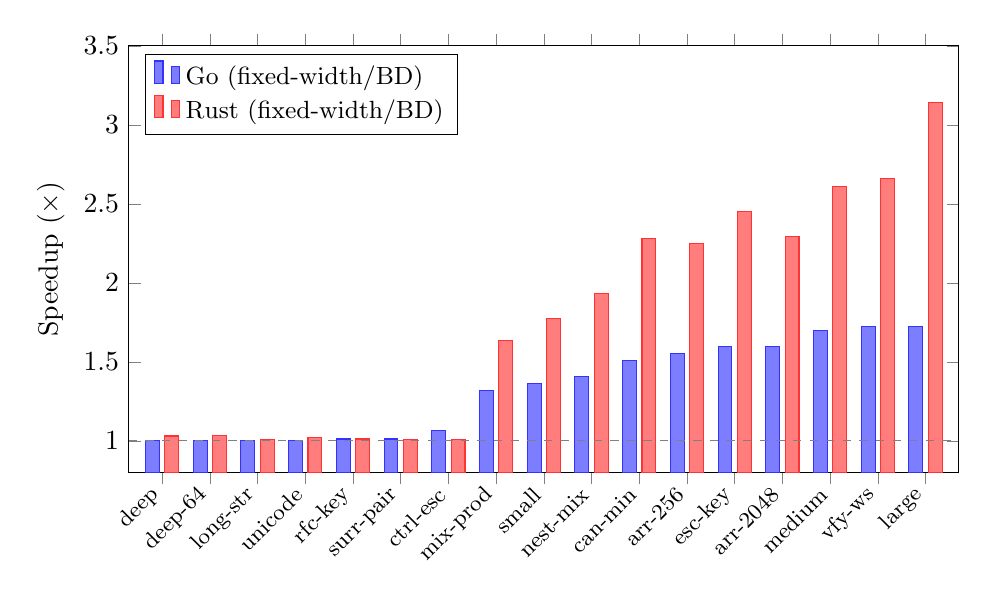
\begin{tikzpicture}
\begin{axis}[
    ybar,
    bar width=5pt,
    width=\textwidth,
    height=7cm,
    ylabel={Speedup ($\times$)},
    xtick={1,2,3,4,5,6,7,8,9,10,11,12,13,14,15,16,17},
    xticklabels={
        deep,
        deep-64,
        long-str,
        unicode,
        rfc-key,
        surr-pair,
        ctrl-esc,
        mix-prod,
        small,
        nest-mix,
        can-min,
        arr-256,
        esc-key,
        arr-2048,
        medium,
        vfy-ws,
        large},
    x tick label style={rotate=45, anchor=east, font=\footnotesize},
    ymin=0.8,
    ymax=3.5,
    xmin=0.3, xmax=17.7,
    ytick={1.0, 1.5, 2.0, 2.5, 3.0, 3.5},
    legend style={at={(0.02,0.98)}, anchor=north west, font=\small},
    legend cell align={left},
    every axis plot/.append style={fill opacity=0.85},
    clip=false,
]
% Go within-language (schubfach-vs-bd), sorted by Go speedup
% Pure-numeric outliers (numeric-boundary, number-heavy) shown separately in §8.5
\addplot[fill=blue!60, draw=blue!80] coordinates {
    (1, 1.000)
    (2, 1.000)
    (3, 1.001)
    (4, 1.003)
    (5, 1.012)
    (6, 1.012)
    (7, 1.065)
    (8, 1.320)
    (9, 1.364)
    (10, 1.408)
    (11, 1.509)
    (12, 1.552)
    (13, 1.595)
    (14, 1.599)
    (15, 1.698)
    (16, 1.721)
    (17, 1.724)
};
% Rust within-language (schubfach-vs-bd)
\addplot[fill=red!60, draw=red!80] coordinates {
    (1, 1.031)
    (2, 1.034)
    (3, 1.008)
    (4, 1.022)
    (5, 1.012)
    (6, 1.011)
    (7, 1.006)
    (8, 1.633)
    (9, 1.776)
    (10, 1.933)
    (11, 2.281)
    (12, 2.247)
    (13, 2.450)
    (14, 2.292)
    (15, 2.611)
    (16, 2.662)
    (17, 3.142)
};
\legend{Go (fixed-width/BD), Rust (fixed-width/BD)}
% Reference line at 1.0x
\draw[dashed, gray, thin] (axis cs:0.3,1.0) -- (axis cs:17.7,1.0);
\end{axis}
\end{tikzpicture}
\caption{API benchmark speedup of fixed-width over \burgerdybvig by
workload (canonicalize mode, \schubfach shown as representative;
\ryualg and \dragonbox produce equivalent ratios per
\S\ref{sec:results}).  Workloads sorted by Go speedup.  Values
above the dashed line indicate the fixed-width algorithm is faster.
Two pure-numeric workloads (\texttt{numeric-boundary} and
\texttt{number-heavy}) are presented separately in
\S\ref{sec:discussion} due to their degenerate number density
($\nu = 100\%$).  Number-dense workloads (right side) show the
largest advantage in both languages, consistent with a shared
algorithmic cause rather than language-specific runtime effects.}
\label{fig:api-speedup}
\end{figure*}


\subsection{Fixed-Width Algorithm Equivalence}

A central finding is that the three fixed-width algorithms (\schubfach,
\ryualg, \dragonbox) perform within 1--8\% of each other across both
languages and all workloads.  In Go API benchmarks, within-fixed-width
comparisons (go:schubfach-vs-ryu, go:schubfach-vs-dragonbox,
go:ryu-vs-dragonbox) show speedups of ${\leq}1.02\times$ with few
BH-significant differences.  In Rust, the same pattern holds, with
occasional small differences (${\leq}1.13\times$) reflecting
compilation artifacts rather than algorithmic cost.

This equivalence confirms that the dominant performance axis is
\emph{fixed-width vs.\ multiprecision}, not the choice among
fixed-width algorithms.

\subsection{CLI Benchmarks}

CLI benchmarks capture end-to-end pipeline cost including process
startup, argument parsing, file I/O, and output serialization.  Estimated
process startup overhead (approximately 1.3\,ms for Go, 0.5\,ms for Rust)
dominates for smaller workloads, attenuating the algorithmic signal
observed in API benchmarks.

Table~\ref{tab:cli-summary} summarizes the key CLI results.
Figure~\ref{fig:cli-significance} shows the end-to-end speedup with
BH-significance markers.  Full results appear in
Appendix~\ref{sec:appendix-tables}.

% Auto-generated by scripts/generate-paper-tables.go
\begin{table}[htbp]
\caption{CLI benchmark summary: within-language comparisons (canonicalize mode, $n{=}15$, 3 warmup discarded).}
\label{tab:cli-summary}
\centering\small
\begin{tabular}{llrrrr}
\toprule
Pair & Workload & Impl A (ms) & Impl B (ms) & Speedup & Winner \\
\midrule
go:schubfach-vs-bd & array-2048 & 5.466 & 7.063 & 1.29$\times$ & schubfach \\
go:schubfach-vs-bd & array-256 & 1.923 & 2.167 & 1.13$\times$ & schubfach \\
go:schubfach-vs-bd & canonical-minimal & 1.510 & 1.565 & 1.04$\times$ & schubfach \\
go:schubfach-vs-bd & control-escapes & 1.380 & 1.673 & 1.21$\times$ & schubfach \\
go:schubfach-vs-bd & deep-64 & 1.467 & 1.638 & 1.12$\times$ & schubfach \\
go:schubfach-vs-bd & escaped-key-order & 1.549 & 1.531 & 1.01$\times$ & json-canon \\
go:schubfach-vs-bd & long-string & 1.409 & 1.692 & 1.20$\times$ & schubfach \\
go:schubfach-vs-bd & nested-mixed & 1.511 & 1.497 & 1.01$\times$ & json-canon \\
go:schubfach-vs-bd & numeric-boundary & 1.537 & 1.706 & 1.11$\times$ & schubfach \\
go:schubfach-vs-bd & rfc-key-sorting & 1.561 & 1.608 & 1.03$\times$ & schubfach \\
go:schubfach-vs-bd & small & 1.450 & 1.449 & 1.00$\times$ & json-canon \\
go:schubfach-vs-bd & surrogate-pair & 1.510 & 1.524 & 1.01$\times$ & schubfach \\
go:schubfach-vs-bd & unicode & 1.597 & 1.470 & 1.09$\times$ & json-canon \\
go:schubfach-vs-bd & verify-whitespace & 1.455 & 1.614 & 1.11$\times$ & schubfach \\
rs:schubfach-vs-bd & array-2048 & 2.606 & 4.584 & 1.76$\times$ & schubfach-rs \\
rs:schubfach-vs-bd & array-256 & 0.828 & 1.152 & 1.39$\times$ & schubfach-rs \\
rs:schubfach-vs-bd & canonical-minimal & 0.546 & 0.582 & 1.07$\times$ & schubfach-rs \\
rs:schubfach-vs-bd & control-escapes & 0.531 & 0.594 & 1.12$\times$ & schubfach-rs \\
rs:schubfach-vs-bd & deep-64 & 0.564 & 0.647 & 1.15$\times$ & schubfach-rs \\
rs:schubfach-vs-bd & escaped-key-order & 0.573 & 0.712 & 1.24$\times$ & schubfach-rs \\
rs:schubfach-vs-bd & long-string & 0.605 & 0.636 & 1.05$\times$ & schubfach-rs \\
rs:schubfach-vs-bd & nested-mixed & 0.555 & 0.644 & 1.16$\times$ & schubfach-rs \\
rs:schubfach-vs-bd & numeric-boundary & 0.543 & 0.738 & 1.36$\times$ & schubfach-rs \\
rs:schubfach-vs-bd & rfc-key-sorting & 0.535 & 0.588 & 1.10$\times$ & schubfach-rs \\
rs:schubfach-vs-bd & small & 0.530 & 0.642 & 1.21$\times$ & schubfach-rs \\
rs:schubfach-vs-bd & surrogate-pair & 0.536 & 0.603 & 1.12$\times$ & schubfach-rs \\
rs:schubfach-vs-bd & unicode & 0.534 & 0.612 & 1.15$\times$ & schubfach-rs \\
rs:schubfach-vs-bd & verify-whitespace & 0.559 & 0.691 & 1.24$\times$ & schubfach-rs \\
\bottomrule
\multicolumn{6}{l}{\footnotesize Full results including verify mode and cross-language pairs in Appendix~\ref{sec:appendix-tables}.} \\
\end{tabular}
\end{table}


\begin{figure*}[htbp]
\centering
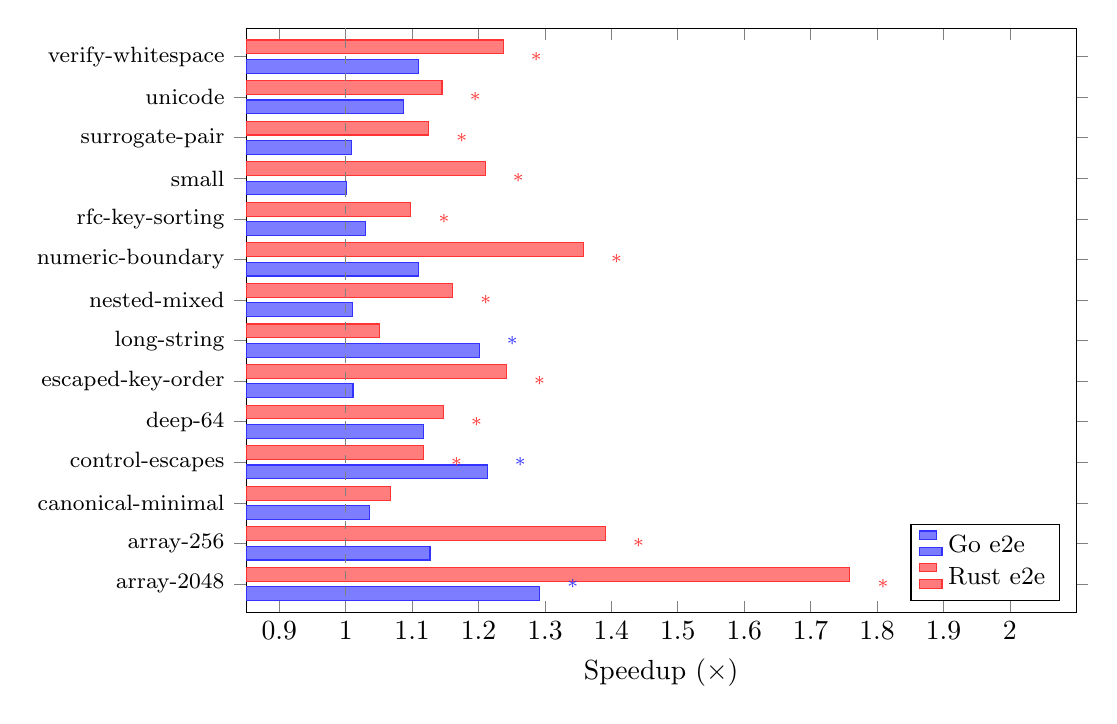
\begin{tikzpicture}
\begin{axis}[
    xbar,
    bar width=5pt,
    width=\textwidth,
    height=9cm,
    xlabel={Speedup ($\times$)},
    ytick={1,2,3,4,5,6,7,8,9,10,11,12,13,14},
    yticklabels={
        array-2048,
        array-256,
        canonical-minimal,
        control-escapes,
        deep-64,
        escaped-key-order,
        long-string,
        nested-mixed,
        numeric-boundary,
        rfc-key-sorting,
        small,
        surrogate-pair,
        unicode,
        verify-whitespace},
    y tick label style={font=\footnotesize},
    xmin=0.85,
    xmax=2.1,
    ymin=0.3, ymax=14.7,
    xtick={0.9, 1.0, 1.1, 1.2, 1.3, 1.4, 1.5, 1.6, 1.7, 1.8, 1.9, 2.0},
    legend style={at={(0.98,0.02)}, anchor=south east, font=\small},
    legend cell align={left},
    every axis plot/.append style={fill opacity=0.85},
    clip=false,
]
% Go CLI e2e canonicalize
\addplot[fill=blue!60, draw=blue!80] coordinates {
    (1.292, 1)
    (1.127, 2)
    (1.036, 3)
    (1.213, 4)
    (1.117, 5)
    (1.011, 6)
    (1.201, 7)
    (1.010, 8)
    (1.110, 9)
    (1.030, 10)
    (1.001, 11)
    (1.009, 12)
    (1.087, 13)
    (1.109, 14)
};
% Rust CLI e2e canonicalize
\addplot[fill=red!60, draw=red!80] coordinates {
    (1.759, 1)
    (1.391, 2)
    (1.067, 3)
    (1.117, 4)
    (1.147, 5)
    (1.242, 6)
    (1.051, 7)
    (1.161, 8)
    (1.358, 9)
    (1.098, 10)
    (1.210, 11)
    (1.125, 12)
    (1.145, 13)
    (1.237, 14)
};
\legend{Go e2e, Rust e2e}
% Reference line at 1.0x
\draw[dashed, gray, thin] (axis cs:1.0,0.3) -- (axis cs:1.0,14.7);
% BH-significant markers for Go (3 canonicalize: array-2048, control-escapes, long-string)
\node[font=\scriptsize, blue!80] at (axis cs:1.342, 1) {$*$};
\node[font=\scriptsize, blue!80] at (axis cs:1.263, 4) {$*$};
\node[font=\scriptsize, blue!80] at (axis cs:1.251, 7) {$*$};
% BH-significant markers for Rust (12 of 14 canonicalize)
\node[font=\scriptsize, red!80] at (axis cs:1.809, 1) {$*$};
\node[font=\scriptsize, red!80] at (axis cs:1.441, 2) {$*$};
\node[font=\scriptsize, red!80] at (axis cs:1.167, 4) {$*$};
\node[font=\scriptsize, red!80] at (axis cs:1.197, 5) {$*$};
\node[font=\scriptsize, red!80] at (axis cs:1.292, 6) {$*$};
\node[font=\scriptsize, red!80] at (axis cs:1.211, 8) {$*$};
\node[font=\scriptsize, red!80] at (axis cs:1.408, 9) {$*$};
\node[font=\scriptsize, red!80] at (axis cs:1.148, 10) {$*$};
\node[font=\scriptsize, red!80] at (axis cs:1.260, 11) {$*$};
\node[font=\scriptsize, red!80] at (axis cs:1.175, 12) {$*$};
\node[font=\scriptsize, red!80] at (axis cs:1.195, 13) {$*$};
\node[font=\scriptsize, red!80] at (axis cs:1.287, 14) {$*$};
\end{axis}
\end{tikzpicture}
\caption{CLI end-to-end speedup of \schubfach over \burgerdybvig by
workload (canonicalize mode, 15~repetitions each).  Asterisks ($*$) mark
BH-significant comparisons ($q < 0.05$).  The Rust within-language pair
achieves significance on 12 of 14~workloads; the Go pair on 3 of
14~workloads (canonicalize mode).  Process startup overhead
(${\approx}$1.3\,ms Go, ${\approx}$0.5\,ms Rust) attenuates the
algorithmic signal more strongly in Go.}
\label{fig:cli-significance}
\end{figure*}


\subsection{Statistical Comparisons}

Within-language CLI comparisons (canonicalize mode) with BH-corrected
$p$-values, confidence intervals, and effect sizes are reported in
Table~\ref{tab:stats-summary} (Appendix~\ref{sec:appendix-tables}).
The patterns mirror the API results: fixed-width algorithms outperform
\burgerdybvig on number-dense workloads, with smaller effect sizes due
to process startup dilution.  The full 1{,}644-comparison statistical
report appears in the supplementary materials.

\subsection{Cross-Language Validation}

All eight implementations pass the full conformance matrix (776 total
cases: 97~structural tests $\times$ 8~implementations, 0~failures) and
produce byte-identical output on all oracle vectors.  2{,}000
differential fuzz cases yield zero cross-implementation divergences.

The statistical report includes 16 comparison classes organized into
three groups:
\begin{itemize}
\item 6~within-Go algorithm pairs and 6~within-Rust algorithm pairs
      (testing algorithmic effects within each language),
\item 4~cross-language same-algorithm pairs (testing language/runtime
      effects while controlling for algorithm).
\end{itemize}

In CLI end-to-end measurement, Rust implementations are approximately
2--3$\times$ faster than their Go counterparts, primarily due to lower
process startup overhead (Rust native binary vs.\ Go runtime
initialization).  In API benchmarks, the within-Rust algorithmic ordering
replicates the within-Go ordering: all three fixed-width algorithms
outperform \burgerdybvig on number-dense workloads; this replication
of within-language ordering provides evidence that the fixed-width
advantage is not solely attributable to language-specific runtime
characteristics.

This decomposition separates algorithmic effects from language/runtime
effects and directly addresses language-specific performance threats.

\subsection{Differential Fuzzing}

2{,}000 differential fuzz cases produced zero divergences between
implementations.

\section{Discussion}
\label{sec:discussion}

\subsection{Workload-Dependent Behavior}

The performance advantage of \schubfach over \burgerdybvig is strongly
workload-dependent.  On number-heavy inputs (e.g., \texttt{numeric-boundary},
\texttt{array-2048}), \schubfach achieves 1.4--2.1$\times$ speedup due
to zero heap allocation in the digit-generation path.  On string-dominant
inputs (e.g., \texttt{long-string}, \texttt{unicode}), the advantage
narrows to $<$5\% because formatting cost is dominated by string
processing and key sorting, amortizing the digit-generation difference.

\subsection{Allocation Cost Attribution}

The \burgerdybvig implementation's \texttt{sync.Pool} partially mitigates
allocation cost by reusing big-integer buffers.  Without pooling, the
difference would be larger.  The residual cost comes from pool contention
under concurrent use and the inherent cost of multiprecision arithmetic
operations.

\subsection{Profile-Level Analysis}

CPU profiling confirms that digit generation consumes 15--40\% of total
canonicalization time depending on workload number density.  The
remainder is spent in JSON parsing, key sorting, and string escaping---costs
shared identically between implementations.

\subsection{Practical Implications}

For applications where canonicalization throughput is critical (e.g.,
high-frequency signature verification of number-heavy payloads),
\schubfach offers meaningful improvement.  For typical mixed-content JSON,
the choice of digit-generation algorithm has minimal practical impact on
end-to-end latency.

\section{Threats to Validity}
\label{sec:threats}

\textbf{Language specificity.}
Both implementations are in Go.  The relative performance of
multiprecision vs.\ fixed-width digit generation may differ in languages
with different allocation models (e.g., C/Rust with stack allocation, or
JVM with generational GC).  The \texttt{sync.Pool} optimization in the
\burgerdybvig implementation is Go-specific.

\textbf{Single-architecture performance data.}
Performance benchmarks run on a single x86-64 machine.  While
cross-architecture \emph{determinism} is verified on arm64 VMs (both
implementations produce byte-identical output), arm64 \emph{performance}
benchmarks are deferred due to lack of bare-metal hardware.  VM overhead
makes cross-architecture performance comparison meaningless.  Future
work should include bare-metal arm64 benchmarks on Graviton, Apple
Silicon, or Ampere hardware.

\textbf{Single JavaScript engine oracle.}
Oracle vectors are generated from V8 (via Node.js).  While ECMA-262
\texttt{Number::toString} semantics are normative and engine-independent,
our vectors are verified against only one engine.  This is mitigated by
exhaustive boundary coverage: 286{,}362 vectors including all subnormals
up to $2^{12}$, all binary64 powers of two, subnormal/normal boundary
neighborhoods, \rfcjcs Appendix~B examples with neighbors, and
pseudorandom fill.

\textbf{Workload representativeness.}
Benchmark workloads are synthetic, designed to bracket the performance
space between number-heavy and string-dominant extremes.  Real-world JSON
payloads may have different number density, nesting depth, and key
length distributions.  However, the control group design (number-only
and string-only workloads) bounds the expected range.

\textbf{sync.Pool mitigation.}
The \burgerdybvig implementation uses \texttt{sync.Pool} to reuse
big-integer buffers, reducing allocation cost.  Without pooling, the
performance gap would be wider.  This reflects realistic production usage
but may understate the theoretical algorithmic advantage of fixed-width
approaches.

\section{Conclusion}
\label{sec:conclusion}

We presented the first empirical comparison of multiprecision
(\burgerdybvig) and fixed-width (\schubfach) digit generation inside a
\rfcjcs/\ecma-constrained JSON canonicalization pipeline.  Our
conformance-gated benchmark methodology ensures that performance
measurements are only meaningful for correct implementations.

Key findings:
\begin{itemize}
\item \schubfach achieves 1.3--1.7$\times$ speedup on number-heavy
      workloads in API benchmarks (1.1--1.3$\times$ end-to-end CLI)
      due to zero heap allocation.
\item The advantage narrows to $<$5\% on string-dominant inputs.
\item Both implementations produce byte-identical output across x86-64
      and arm64.
\item Digit generation accounts for 15--40\% of total canonicalization
      cost depending on number density.
\end{itemize}

The benchmark infrastructure, 286{,}362 oracle vectors, and all raw data
are released as a reproducibility artifact.

\subsection*{Future Work}

Bare-metal arm64 performance benchmarks, additional language
implementations (Rust, C), multi-engine oracle validation (SpiderMonkey,
JavaScriptCore), and workload characterization from production JSON
corpora.


\section*{Data Availability Statement}

All data, software, and oracle vectors are freely available online.
The benchmark infrastructure, all eight implementations, workload manifests,
and oracle generation scripts are available at the accompanying
repository.\footnote{Repository URL and Zenodo DOI to be inserted for
camera-ready version.}  Oracle vector checksums (SHA-256) are documented in
\texttt{PROVENANCE.json} files accompanying each implementation.

\section*{Author Contributions}

Following the CRediT (Contributor Roles Taxonomy) format:
\textit{Mark Lenhardt:} conceptualization; methodology;
software; validation; formal analysis; investigation; data curation;
writing---original draft; writing---review and editing; visualization.

\bibliographystyle{plain}
\bibliography{references}

\clearpage
\appendix
\section{Full Benchmark Data}
\label{sec:appendix-tables}

This appendix contains the complete benchmark results.  Summary tables
appear in the main text (\S\ref{sec:results}); the full data are
provided here for reproducibility.

\emph{Note:} Rust benchmark rows report \texttt{0~B/op} and
\texttt{0~allocs/op} because Rust lacks Go-style per-operation allocator
statistics.  These values mean ``not measured,'' not ``zero
allocations'' (see \S\ref{sec:discussion}).

\begin{landscape}

\subsection{Full API Benchmarks}
% Auto-generated by scripts/generate-paper-tables.go
\scriptsize
\begin{longtable}{lllrrrrr}
\caption{API benchmark results (mean of $n=10$ iterations).}
\label{tab:api-benchmarks}\\
\toprule
Pair & Workload & Mode & \multicolumn{2}{c}{ns/op} & Speedup & $\Delta$allocs/op & $\Delta$B/op \\
\midrule
\endfirsthead
\toprule
Pair & Workload & Mode & \multicolumn{2}{c}{ns/op} & Speedup & $\Delta$allocs/op & $\Delta$B/op \\
\midrule
\endhead
\midrule
\multicolumn{8}{r}{\textit{Continued on next page}} \\
\endfoot
\bottomrule
\multicolumn{8}{l}{\footnotesize B/op = bytes allocated per operation. allocs/op = heap allocations per operation.} \\
\multicolumn{8}{l}{\footnotesize $\Delta$ columns show Impl B $-$ Impl A for each pair.} \\
\endlastfoot
go:schubfach-vs-bd & array-2048 & canonicalize & 2538189 & 4058559 & 1.60$\times$ & +8210 & +186691 \\
go:schubfach-vs-bd & array-256 & canonicalize & 304201 & 472012 & 1.55$\times$ & +1020 & +24976 \\
go:schubfach-vs-bd & canonical-minimal & canonicalize & 351 & 530 & 1.51$\times$ & +0 & +0 \\
go:schubfach-vs-bd & control-escapes & canonicalize & 1333 & 1252 & 1.06$\times$ & +0 & +0 \\
go:schubfach-vs-bd & deep & canonicalize & 36663 & 36648 & 1.00$\times$ & +0 & +0 \\
go:schubfach-vs-bd & deep-64 & canonicalize & 16218 & 16221 & 1.00$\times$ & +0 & +0 \\
go:schubfach-vs-bd & escaped-key-order & canonicalize & 706 & 1125 & 1.59$\times$ & +2 & +41 \\
go:schubfach-vs-bd & large & canonicalize & 11952645 & 20608504 & 1.72$\times$ & +32792 & +663257 \\
go:schubfach-vs-bd & long-string & canonicalize & 75536 & 75430 & 1.00$\times$ & +0 & +0 \\
go:schubfach-vs-bd & medium & canonicalize & 341381 & 579627 & 1.70$\times$ & +1014 & +21130 \\
go:schubfach-vs-bd & mixed-prod & canonicalize & 135688 & 179064 & 1.32$\times$ & +255 & +6237 \\
go:schubfach-vs-bd & nested-mixed & canonicalize & 2177 & 3065 & 1.41$\times$ & +4 & +85 \\
go:schubfach-vs-bd & number-heavy & canonicalize & 13812 & 21307 & 1.54$\times$ & +20 & +830 \\
go:schubfach-vs-bd & numeric-boundary & canonicalize & 12603 & 18700 & 1.48$\times$ & +14 & +706 \\
go:schubfach-vs-bd & rfc-key-sorting & canonicalize & 2999 & 2963 & 1.01$\times$ & +0 & +0 \\
go:schubfach-vs-bd & small & canonicalize & 1235 & 1685 & 1.36$\times$ & +2 & +50 \\
go:schubfach-vs-bd & surrogate-pair & canonicalize & 646 & 638 & 1.01$\times$ & +0 & +0 \\
go:schubfach-vs-bd & unicode & canonicalize & 1546 & 1541 & 1.00$\times$ & +0 & +0 \\
go:schubfach-vs-bd & verify-whitespace & canonicalize & 906 & 1559 & 1.72$\times$ & +4 & +82 \\
go:schubfach-vs-bd & canonical/array-2048 & verify & 2475365 & 4019281 & 1.62$\times$ & +8208 & +186522 \\
go:schubfach-vs-bd & canonical/array-256 & verify & 314132 & 483772 & 1.54$\times$ & +1021 & +25208 \\
go:schubfach-vs-bd & canonical/canonical-minimal & verify & 359 & 548 & 1.53$\times$ & +0 & +0 \\
go:schubfach-vs-bd & canonical/control-escapes & verify & 1319 & 1277 & 1.03$\times$ & +0 & +0 \\
go:schubfach-vs-bd & canonical/deep & verify & 37929 & 38260 & 1.01$\times$ & +0 & +0 \\
go:schubfach-vs-bd & canonical/deep-64 & verify & 16664 & 16930 & 1.02$\times$ & +0 & +0 \\
go:schubfach-vs-bd & canonical/escaped-key-order & verify & 685 & 1134 & 1.65$\times$ & +2 & +41 \\
go:schubfach-vs-bd & canonical/large & verify & 11465484 & 19941996 & 1.74$\times$ & +32790 & +662980 \\
go:schubfach-vs-bd & canonical/long-string & verify & 76827 & 77335 & 1.01$\times$ & +0 & +0 \\
go:schubfach-vs-bd & canonical/medium & verify & 338837 & 576583 & 1.70$\times$ & +1015 & +21370 \\
go:schubfach-vs-bd & canonical/mixed-prod & verify & 132472 & 175149 & 1.32$\times$ & +255 & +6323 \\
go:schubfach-vs-bd & canonical/nested-mixed & verify & 2203 & 3098 & 1.41$\times$ & +4 & +86 \\
go:schubfach-vs-bd & canonical/number-heavy & verify & 13838 & 21562 & 1.56$\times$ & +20 & +834 \\
go:schubfach-vs-bd & canonical/numeric-boundary & verify & 12820 & 18752 & 1.46$\times$ & +14 & +709 \\
go:schubfach-vs-bd & canonical/rfc-key-sorting & verify & 2840 & 2831 & 1.00$\times$ & +0 & +0 \\
go:schubfach-vs-bd & canonical/small & verify & 1214 & 1651 & 1.36$\times$ & +2 & +51 \\
go:schubfach-vs-bd & canonical/surrogate-pair & verify & 651 & 653 & 1.00$\times$ & +0 & +0 \\
go:schubfach-vs-bd & canonical/unicode & verify & 1540 & 1544 & 1.00$\times$ & +0 & +0 \\
go:schubfach-vs-bd & canonical/verify-whitespace & verify & 929 & 1588 & 1.71$\times$ & +4 & +82 \\
go:schubfach-vs-bd & noncanonical/control-escapes & verify & 1318 & 1257 & 1.05$\times$ & +0 & +0 \\
go:schubfach-vs-bd & noncanonical/escaped-key-order & verify & 701 & 1128 & 1.61$\times$ & +2 & +41 \\
go:schubfach-vs-bd & noncanonical/large & verify & 11919728 & 20550017 & 1.72$\times$ & +32792 & +663497 \\
go:schubfach-vs-bd & noncanonical/medium & verify & 343792 & 574323 & 1.67$\times$ & +1014 & +21131 \\
go:schubfach-vs-bd & noncanonical/mixed-prod & verify & 137067 & 177569 & 1.30$\times$ & +255 & +6226 \\
go:schubfach-vs-bd & noncanonical/nested-mixed & verify & 2191 & 3070 & 1.40$\times$ & +4 & +85 \\
go:schubfach-vs-bd & noncanonical/number-heavy & verify & 13881 & 21352 & 1.54$\times$ & +20 & +830 \\
go:schubfach-vs-bd & noncanonical/numeric-boundary & verify & 12851 & 18650 & 1.45$\times$ & +14 & +706 \\
go:schubfach-vs-bd & noncanonical/rfc-key-sorting & verify & 3015 & 2959 & 1.02$\times$ & +0 & +0 \\
go:schubfach-vs-bd & noncanonical/small & verify & 1250 & 1668 & 1.33$\times$ & +2 & +50 \\
go:schubfach-vs-bd & noncanonical/surrogate-pair & verify & 656 & 643 & 1.02$\times$ & +0 & +0 \\
go:schubfach-vs-bd & noncanonical/unicode & verify & 1566 & 1547 & 1.01$\times$ & +0 & +0 \\
go:schubfach-vs-bd & noncanonical/verify-whitespace & verify & 922 & 1554 & 1.69$\times$ & +4 & +82 \\
rs:schubfach-vs-bd & array-2048 & canonicalize & 1261394 & 2891090 & 2.29$\times$ & +0 & +0 \\
rs:schubfach-vs-bd & array-256 & canonicalize & 147811 & 332147 & 2.25$\times$ & +0 & +0 \\
rs:schubfach-vs-bd & canonical-minimal & canonicalize & 183 & 418 & 2.28$\times$ & +0 & +0 \\
rs:schubfach-vs-bd & control-escapes & canonicalize & 620 & 617 & 1.01$\times$ & +0 & +0 \\
rs:schubfach-vs-bd & deep & canonicalize & 26488 & 25683 & 1.03$\times$ & +0 & +0 \\
rs:schubfach-vs-bd & deep-64 & canonicalize & 9482 & 9174 & 1.03$\times$ & +0 & +0 \\
rs:schubfach-vs-bd & escaped-key-order & canonicalize & 303 & 742 & 2.45$\times$ & +0 & +0 \\
rs:schubfach-vs-bd & large & canonicalize & 5132778 & 16125242 & 3.14$\times$ & +0 & +0 \\
rs:schubfach-vs-bd & long-string & canonicalize & 17188 & 17328 & 1.01$\times$ & +0 & +0 \\
rs:schubfach-vs-bd & medium & canonicalize & 166916 & 435894 & 2.61$\times$ & +0 & +0 \\
rs:schubfach-vs-bd & mixed-prod & canonicalize & 65576 & 107081 & 1.63$\times$ & +0 & +0 \\
rs:schubfach-vs-bd & nested-mixed & canonicalize & 878 & 1698 & 1.93$\times$ & +0 & +0 \\
rs:schubfach-vs-bd & number-heavy & canonicalize & 1403 & 11464 & 8.17$\times$ & +0 & +0 \\
rs:schubfach-vs-bd & numeric-boundary & canonicalize & 955 & 8774 & 9.18$\times$ & +0 & +0 \\
rs:schubfach-vs-bd & rfc-key-sorting & canonicalize & 1278 & 1263 & 1.01$\times$ & +0 & +0 \\
rs:schubfach-vs-bd & small & canonicalize & 578 & 1026 & 1.78$\times$ & +0 & +0 \\
rs:schubfach-vs-bd & surrogate-pair & canonicalize & 273 & 276 & 1.01$\times$ & +0 & +0 \\
rs:schubfach-vs-bd & unicode & canonicalize & 1686 & 1650 & 1.02$\times$ & +0 & +0 \\
rs:schubfach-vs-bd & verify-whitespace & canonicalize & 369 & 983 & 2.66$\times$ & +0 & +0 \\
rs:schubfach-vs-bd & canonical/array-2048 & verify & 1178769 & 2920389 & 2.48$\times$ & +0 & +0 \\
rs:schubfach-vs-bd & canonical/array-256 & verify & 132345 & 316436 & 2.39$\times$ & +0 & +0 \\
rs:schubfach-vs-bd & canonical/canonical-minimal & verify & 181 & 421 & 2.32$\times$ & +0 & +0 \\
rs:schubfach-vs-bd & canonical/control-escapes & verify & 586 & 608 & 1.04$\times$ & +0 & +0 \\
rs:schubfach-vs-bd & canonical/deep & verify & 26824 & 25174 & 1.07$\times$ & +0 & +0 \\
rs:schubfach-vs-bd & canonical/deep-64 & verify & 9156 & 9266 & 1.01$\times$ & +0 & +0 \\
rs:schubfach-vs-bd & canonical/escaped-key-order & verify & 291 & 712 & 2.45$\times$ & +0 & +0 \\
rs:schubfach-vs-bd & canonical/large & verify & 5375262 & 16330345 & 3.04$\times$ & +0 & +0 \\
rs:schubfach-vs-bd & canonical/long-string & verify & 17299 & 17580 & 1.02$\times$ & +0 & +0 \\
rs:schubfach-vs-bd & canonical/medium & verify & 143326 & 437556 & 3.05$\times$ & +0 & +0 \\
rs:schubfach-vs-bd & canonical/mixed-prod & verify & 65487 & 109623 & 1.67$\times$ & +0 & +0 \\
rs:schubfach-vs-bd & canonical/nested-mixed & verify & 856 & 1666 & 1.95$\times$ & +0 & +0 \\
rs:schubfach-vs-bd & canonical/number-heavy & verify & 1388 & 11075 & 7.98$\times$ & +0 & +0 \\
rs:schubfach-vs-bd & canonical/numeric-boundary & verify & 961 & 8726 & 9.08$\times$ & +0 & +0 \\
rs:schubfach-vs-bd & canonical/rfc-key-sorting & verify & 1322 & 1360 & 1.03$\times$ & +0 & +0 \\
rs:schubfach-vs-bd & canonical/small & verify & 579 & 1016 & 1.75$\times$ & +0 & +0 \\
rs:schubfach-vs-bd & canonical/surrogate-pair & verify & 284 & 291 & 1.02$\times$ & +0 & +0 \\
rs:schubfach-vs-bd & canonical/unicode & verify & 1725 & 1648 & 1.05$\times$ & +0 & +0 \\
rs:schubfach-vs-bd & canonical/verify-whitespace & verify & 353 & 967 & 2.74$\times$ & +0 & +0 \\
schubfach:go-vs-rs & array-2048 & canonicalize & 2538189 & 1261394 & 2.01$\times$ & -49134 & -4939278 \\
schubfach:go-vs-rs & array-256 & canonicalize & 304201 & 147811 & 2.06$\times$ & -6131 & -604880 \\
schubfach:go-vs-rs & canonical-minimal & canonicalize & 351 & 183 & 1.92$\times$ & -8 & -504 \\
schubfach:go-vs-rs & control-escapes & canonicalize & 1333 & 620 & 2.15$\times$ & -21 & -2064 \\
schubfach:go-vs-rs & deep & canonicalize & 36663 & 26488 & 1.38$\times$ & -843 & -58960 \\
schubfach:go-vs-rs & deep-64 & canonicalize & 16218 & 9482 & 1.71$\times$ & -387 & -26904 \\
schubfach:go-vs-rs & escaped-key-order & canonicalize & 706 & 303 & 2.33$\times$ & -14 & -1168 \\
schubfach:go-vs-rs & large & canonicalize & 11952645 & 5132778 & 2.33$\times$ & -204776 & -20914304 \\
schubfach:go-vs-rs & long-string & canonicalize & 75536 & 17188 & 4.39$\times$ & -14 & -35948 \\
schubfach:go-vs-rs & medium & canonicalize & 341381 & 166916 & 2.05$\times$ & -6380 & -618687 \\
schubfach:go-vs-rs & mixed-prod & canonicalize & 135688 & 65576 & 2.07$\times$ & -2340 & -256989 \\
schubfach:go-vs-rs & nested-mixed & canonicalize & 2177 & 878 & 2.48$\times$ & -45 & -4128 \\
schubfach:go-vs-rs & number-heavy & canonicalize & 13812 & 1403 & 9.84$\times$ & -60 & -4576 \\
schubfach:go-vs-rs & numeric-boundary & canonicalize & 12603 & 955 & 13.19$\times$ & -38 & -3208 \\
schubfach:go-vs-rs & rfc-key-sorting & canonicalize & 2999 & 1278 & 2.35$\times$ & -47 & -4256 \\
schubfach:go-vs-rs & small & canonicalize & 1235 & 578 & 2.14$\times$ & -22 & -2152 \\
schubfach:go-vs-rs & surrogate-pair & canonicalize & 646 & 273 & 2.37$\times$ & -14 & -1168 \\
schubfach:go-vs-rs & unicode & canonicalize & 1546 & 1686 & 1.09$\times$ & -19 & -2019 \\
schubfach:go-vs-rs & verify-whitespace & canonicalize & 906 & 369 & 2.45$\times$ & -19 & -1576 \\
schubfach:go-vs-rs & canonical/array-2048 & verify & 2475365 & 1178769 & 2.10$\times$ & -49134 & -4939271 \\
schubfach:go-vs-rs & canonical/array-256 & verify & 314132 & 132345 & 2.37$\times$ & -6131 & -604881 \\
schubfach:go-vs-rs & canonical/canonical-minimal & verify & 359 & 181 & 1.98$\times$ & -8 & -504 \\
schubfach:go-vs-rs & canonical/control-escapes & verify & 1319 & 586 & 2.25$\times$ & -21 & -2064 \\
schubfach:go-vs-rs & canonical/deep & verify & 37929 & 26824 & 1.41$\times$ & -843 & -58960 \\
schubfach:go-vs-rs & canonical/deep-64 & verify & 16664 & 9156 & 1.82$\times$ & -387 & -26904 \\
schubfach:go-vs-rs & canonical/escaped-key-order & verify & 685 & 291 & 2.36$\times$ & -14 & -1160 \\
schubfach:go-vs-rs & canonical/large & verify & 11465484 & 5375262 & 2.13$\times$ & -204776 & -20914288 \\
schubfach:go-vs-rs & canonical/long-string & verify & 76827 & 17299 & 4.44$\times$ & -14 & -35948 \\
schubfach:go-vs-rs & canonical/medium & verify & 338837 & 143326 & 2.36$\times$ & -6380 & -618688 \\
schubfach:go-vs-rs & canonical/mixed-prod & verify & 132472 & 65487 & 2.02$\times$ & -2340 & -256989 \\
schubfach:go-vs-rs & canonical/nested-mixed & verify & 2203 & 856 & 2.58$\times$ & -45 & -4128 \\
schubfach:go-vs-rs & canonical/number-heavy & verify & 13838 & 1388 & 9.97$\times$ & -60 & -4576 \\
schubfach:go-vs-rs & canonical/numeric-boundary & verify & 12820 & 961 & 13.34$\times$ & -38 & -3208 \\
schubfach:go-vs-rs & canonical/rfc-key-sorting & verify & 2840 & 1322 & 2.15$\times$ & -42 & -4240 \\
schubfach:go-vs-rs & canonical/small & verify & 1214 & 579 & 2.10$\times$ & -22 & -2152 \\
schubfach:go-vs-rs & canonical/surrogate-pair & verify & 651 & 284 & 2.29$\times$ & -14 & -1160 \\
schubfach:go-vs-rs & canonical/unicode & verify & 1540 & 1725 & 1.12$\times$ & -19 & -2003 \\
schubfach:go-vs-rs & canonical/verify-whitespace & verify & 929 & 353 & 2.63$\times$ & -19 & -1576 \\
bd:go-vs-rs & array-2048 & canonicalize & 4058559 & 2891090 & 1.40$\times$ & -57344 & -5125968 \\
bd:go-vs-rs & array-256 & canonicalize & 472012 & 332147 & 1.42$\times$ & -7151 & -629856 \\
bd:go-vs-rs & canonical-minimal & canonicalize & 530 & 418 & 1.27$\times$ & -8 & -504 \\
bd:go-vs-rs & control-escapes & canonicalize & 1252 & 617 & 2.03$\times$ & -21 & -2064 \\
bd:go-vs-rs & deep & canonicalize & 36648 & 25683 & 1.43$\times$ & -843 & -58960 \\
bd:go-vs-rs & deep-64 & canonicalize & 16221 & 9174 & 1.77$\times$ & -387 & -26904 \\
bd:go-vs-rs & escaped-key-order & canonicalize & 1125 & 742 & 1.52$\times$ & -16 & -1209 \\
bd:go-vs-rs & large & canonicalize & 20608504 & 16125242 & 1.28$\times$ & -237568 & -21577561 \\
bd:go-vs-rs & long-string & canonicalize & 75430 & 17328 & 4.35$\times$ & -14 & -35948 \\
bd:go-vs-rs & medium & canonicalize & 579627 & 435894 & 1.33$\times$ & -7394 & -639818 \\
bd:go-vs-rs & mixed-prod & canonicalize & 179064 & 107081 & 1.67$\times$ & -2595 & -263226 \\
bd:go-vs-rs & nested-mixed & canonicalize & 3065 & 1698 & 1.81$\times$ & -49 & -4213 \\
bd:go-vs-rs & number-heavy & canonicalize & 21307 & 11464 & 1.86$\times$ & -80 & -5406 \\
bd:go-vs-rs & numeric-boundary & canonicalize & 18700 & 8774 & 2.13$\times$ & -52 & -3914 \\
bd:go-vs-rs & rfc-key-sorting & canonicalize & 2963 & 1263 & 2.35$\times$ & -47 & -4256 \\
bd:go-vs-rs & small & canonicalize & 1685 & 1026 & 1.64$\times$ & -24 & -2202 \\
bd:go-vs-rs & surrogate-pair & canonicalize & 638 & 276 & 2.31$\times$ & -14 & -1168 \\
bd:go-vs-rs & unicode & canonicalize & 1541 & 1650 & 1.07$\times$ & -19 & -2019 \\
bd:go-vs-rs & verify-whitespace & canonicalize & 1559 & 983 & 1.59$\times$ & -23 & -1658 \\
bd:go-vs-rs & canonical/array-2048 & verify & 4019281 & 2920389 & 1.38$\times$ & -57342 & -5125793 \\
bd:go-vs-rs & canonical/array-256 & verify & 483772 & 316436 & 1.53$\times$ & -7152 & -630089 \\
bd:go-vs-rs & canonical/canonical-minimal & verify & 548 & 421 & 1.30$\times$ & -8 & -504 \\
bd:go-vs-rs & canonical/control-escapes & verify & 1277 & 608 & 2.10$\times$ & -21 & -2064 \\
bd:go-vs-rs & canonical/deep & verify & 38260 & 25174 & 1.52$\times$ & -843 & -58960 \\
bd:go-vs-rs & canonical/deep-64 & verify & 16930 & 9266 & 1.83$\times$ & -387 & -26904 \\
bd:go-vs-rs & canonical/escaped-key-order & verify & 1134 & 712 & 1.59$\times$ & -16 & -1201 \\
bd:go-vs-rs & canonical/large & verify & 19941996 & 16330345 & 1.22$\times$ & -237565 & -21577268 \\
bd:go-vs-rs & canonical/long-string & verify & 77335 & 17580 & 4.40$\times$ & -14 & -35948 \\
bd:go-vs-rs & canonical/medium & verify & 576583 & 437556 & 1.32$\times$ & -7395 & -640059 \\
bd:go-vs-rs & canonical/mixed-prod & verify & 175149 & 109623 & 1.60$\times$ & -2595 & -263312 \\
bd:go-vs-rs & canonical/nested-mixed & verify & 3098 & 1666 & 1.86$\times$ & -49 & -4214 \\
bd:go-vs-rs & canonical/number-heavy & verify & 21562 & 11075 & 1.95$\times$ & -80 & -5410 \\
bd:go-vs-rs & canonical/numeric-boundary & verify & 18752 & 8726 & 2.15$\times$ & -52 & -3917 \\
bd:go-vs-rs & canonical/rfc-key-sorting & verify & 2831 & 1360 & 2.08$\times$ & -42 & -4240 \\
bd:go-vs-rs & canonical/small & verify & 1651 & 1016 & 1.63$\times$ & -24 & -2203 \\
bd:go-vs-rs & canonical/surrogate-pair & verify & 653 & 291 & 2.24$\times$ & -14 & -1160 \\
bd:go-vs-rs & canonical/unicode & verify & 1544 & 1648 & 1.07$\times$ & -19 & -2003 \\
bd:go-vs-rs & canonical/verify-whitespace & verify & 1588 & 967 & 1.64$\times$ & -23 & -1658 \\
\end{longtable}
\normalsize


\subsection{Full CLI Benchmarks}
% Auto-generated by scripts/generate-paper-tables.go
\scriptsize
\begin{longtable}{lllrrrr}
\caption{CLI benchmark results (end-to-end, $n=15$).}
\label{tab:cli-benchmarks}\\
\toprule
Pair & Workload & Mode & Impl A (ms) & Impl B (ms) & Speedup & Winner \\
\midrule
\endfirsthead
\toprule
Pair & Workload & Mode & Impl A (ms) & Impl B (ms) & Speedup & Winner \\
\midrule
\endhead
\midrule
\multicolumn{7}{r}{\textit{Continued on next page}} \\
\endfoot
\bottomrule
\multicolumn{7}{l}{\footnotesize Speedup = slower/faster mean wall time. $n=15$ repetitions, 3 warmup runs discarded.} \\
\endlastfoot
go:schubfach-vs-bd & array-2048 & canonicalize & 5.642 & 7.202 & 1.28$\times$ & schubfach \\
go:schubfach-vs-bd & array-2048 & verify & 5.694 & 7.125 & 1.25$\times$ & schubfach \\
go:schubfach-vs-bd & array-256 & canonicalize & 1.840 & 2.383 & 1.30$\times$ & schubfach \\
go:schubfach-vs-bd & array-256 & verify & 2.087 & 2.246 & 1.08$\times$ & schubfach \\
go:schubfach-vs-bd & canonical-minimal & canonicalize & 1.378 & 1.655 & 1.20$\times$ & schubfach \\
go:schubfach-vs-bd & canonical-minimal & verify & 1.443 & 1.654 & 1.15$\times$ & schubfach \\
go:schubfach-vs-bd & control-escapes & canonicalize & 1.501 & 1.569 & 1.05$\times$ & schubfach \\
go:schubfach-vs-bd & control-escapes & verify & 1.352 & 1.697 & 1.26$\times$ & schubfach \\
go:schubfach-vs-bd & deep & canonicalize & 1.643 & 1.722 & 1.05$\times$ & schubfach \\
go:schubfach-vs-bd & deep & verify & 1.704 & 1.723 & 1.01$\times$ & schubfach \\
go:schubfach-vs-bd & deep-64 & canonicalize & 1.443 & 1.828 & 1.27$\times$ & schubfach \\
go:schubfach-vs-bd & deep-64 & verify & 1.584 & 1.636 & 1.03$\times$ & schubfach \\
go:schubfach-vs-bd & escaped-key-order & canonicalize & 1.489 & 1.553 & 1.04$\times$ & schubfach \\
go:schubfach-vs-bd & escaped-key-order & verify & 1.543 & 1.546 & 1.00$\times$ & schubfach \\
go:schubfach-vs-bd & large & canonicalize & 16.530 & 24.906 & 1.51$\times$ & schubfach \\
go:schubfach-vs-bd & large & verify & 15.913 & 24.895 & 1.56$\times$ & schubfach \\
go:schubfach-vs-bd & long-string & canonicalize & 1.566 & 1.821 & 1.16$\times$ & schubfach \\
go:schubfach-vs-bd & long-string & verify & 1.791 & 1.912 & 1.07$\times$ & schubfach \\
go:schubfach-vs-bd & medium & canonicalize & 1.986 & 2.659 & 1.34$\times$ & schubfach \\
go:schubfach-vs-bd & medium & verify & 2.143 & 2.531 & 1.18$\times$ & schubfach \\
go:schubfach-vs-bd & mixed-prod & canonicalize & 1.851 & 1.907 & 1.03$\times$ & schubfach \\
go:schubfach-vs-bd & mixed-prod & verify & 1.614 & 1.877 & 1.16$\times$ & schubfach \\
go:schubfach-vs-bd & nested-mixed & canonicalize & 1.481 & 1.613 & 1.09$\times$ & schubfach \\
go:schubfach-vs-bd & nested-mixed & verify & 1.486 & 1.739 & 1.17$\times$ & schubfach \\
go:schubfach-vs-bd & number-heavy & canonicalize & 1.484 & 1.656 & 1.12$\times$ & schubfach \\
go:schubfach-vs-bd & number-heavy & verify & 1.523 & 1.763 & 1.16$\times$ & schubfach \\
go:schubfach-vs-bd & numeric-boundary & canonicalize & 1.578 & 1.556 & 1.01$\times$ & json-canon \\
go:schubfach-vs-bd & numeric-boundary & verify & 1.550 & 1.627 & 1.05$\times$ & schubfach \\
go:schubfach-vs-bd & rfc-key-sorting & canonicalize & 1.442 & 1.564 & 1.08$\times$ & schubfach \\
go:schubfach-vs-bd & rfc-key-sorting & verify & 1.499 & 1.566 & 1.04$\times$ & schubfach \\
go:schubfach-vs-bd & small & canonicalize & 1.453 & 1.588 & 1.09$\times$ & schubfach \\
go:schubfach-vs-bd & small & verify & 1.561 & 1.653 & 1.06$\times$ & schubfach \\
go:schubfach-vs-bd & surrogate-pair & canonicalize & 1.425 & 1.549 & 1.09$\times$ & schubfach \\
go:schubfach-vs-bd & surrogate-pair & verify & 1.546 & 1.469 & 1.05$\times$ & json-canon \\
go:schubfach-vs-bd & unicode & canonicalize & 1.819 & 1.474 & 1.23$\times$ & json-canon \\
go:schubfach-vs-bd & unicode & verify & 1.488 & 1.524 & 1.02$\times$ & schubfach \\
go:schubfach-vs-bd & verify-whitespace & canonicalize & 1.478 & 1.634 & 1.11$\times$ & schubfach \\
go:schubfach-vs-bd & verify-whitespace & verify & 1.457 & 1.785 & 1.23$\times$ & schubfach \\
rs:schubfach-vs-bd & array-2048 & canonicalize & 2.664 & 4.606 & 1.73$\times$ & schubfach-rs \\
rs:schubfach-vs-bd & array-2048 & verify & 2.451 & 4.380 & 1.79$\times$ & schubfach-rs \\
rs:schubfach-vs-bd & array-256 & canonicalize & 0.866 & 1.149 & 1.33$\times$ & schubfach-rs \\
rs:schubfach-vs-bd & array-256 & verify & 0.817 & 1.206 & 1.48$\times$ & schubfach-rs \\
rs:schubfach-vs-bd & canonical-minimal & canonicalize & 0.571 & 0.619 & 1.08$\times$ & schubfach-rs \\
rs:schubfach-vs-bd & canonical-minimal & verify & 0.538 & 0.610 & 1.13$\times$ & schubfach-rs \\
rs:schubfach-vs-bd & control-escapes & canonicalize & 0.559 & 0.644 & 1.15$\times$ & schubfach-rs \\
rs:schubfach-vs-bd & control-escapes & verify & 0.535 & 0.653 & 1.22$\times$ & schubfach-rs \\
rs:schubfach-vs-bd & deep & canonicalize & 0.605 & 0.682 & 1.13$\times$ & schubfach-rs \\
rs:schubfach-vs-bd & deep & verify & 0.648 & 0.694 & 1.07$\times$ & schubfach-rs \\
rs:schubfach-vs-bd & deep-64 & canonicalize & 0.614 & 0.632 & 1.03$\times$ & schubfach-rs \\
rs:schubfach-vs-bd & deep-64 & verify & 0.563 & 0.644 & 1.14$\times$ & schubfach-rs \\
rs:schubfach-vs-bd & escaped-key-order & canonicalize & 0.556 & 0.685 & 1.23$\times$ & schubfach-rs \\
rs:schubfach-vs-bd & escaped-key-order & verify & 0.554 & 0.698 & 1.26$\times$ & schubfach-rs \\
rs:schubfach-vs-bd & large & canonicalize & 7.967 & 18.705 & 2.35$\times$ & schubfach-rs \\
rs:schubfach-vs-bd & large & verify & 7.214 & 18.635 & 2.58$\times$ & schubfach-rs \\
rs:schubfach-vs-bd & long-string & canonicalize & 0.630 & 0.716 & 1.14$\times$ & schubfach-rs \\
rs:schubfach-vs-bd & long-string & verify & 0.647 & 0.667 & 1.03$\times$ & schubfach-rs \\
rs:schubfach-vs-bd & medium & canonicalize & 0.869 & 1.338 & 1.54$\times$ & schubfach-rs \\
rs:schubfach-vs-bd & medium & verify & 0.861 & 1.366 & 1.59$\times$ & schubfach-rs \\
rs:schubfach-vs-bd & mixed-prod & canonicalize & 0.694 & 0.882 & 1.27$\times$ & schubfach-rs \\
rs:schubfach-vs-bd & mixed-prod & verify & 0.717 & 0.865 & 1.21$\times$ & schubfach-rs \\
rs:schubfach-vs-bd & nested-mixed & canonicalize & 0.559 & 0.689 & 1.23$\times$ & schubfach-rs \\
rs:schubfach-vs-bd & nested-mixed & verify & 0.569 & 0.700 & 1.23$\times$ & schubfach-rs \\
rs:schubfach-vs-bd & number-heavy & canonicalize & 0.570 & 0.735 & 1.29$\times$ & schubfach-rs \\
rs:schubfach-vs-bd & number-heavy & verify & 0.568 & 0.732 & 1.29$\times$ & schubfach-rs \\
rs:schubfach-vs-bd & numeric-boundary & canonicalize & 0.562 & 0.736 & 1.31$\times$ & schubfach-rs \\
rs:schubfach-vs-bd & numeric-boundary & verify & 0.546 & 0.718 & 1.31$\times$ & schubfach-rs \\
rs:schubfach-vs-bd & rfc-key-sorting & canonicalize & 0.578 & 0.629 & 1.09$\times$ & schubfach-rs \\
rs:schubfach-vs-bd & rfc-key-sorting & verify & 0.561 & 0.617 & 1.10$\times$ & schubfach-rs \\
rs:schubfach-vs-bd & small & canonicalize & 0.545 & 0.673 & 1.23$\times$ & schubfach-rs \\
rs:schubfach-vs-bd & small & verify & 0.588 & 0.704 & 1.20$\times$ & schubfach-rs \\
rs:schubfach-vs-bd & surrogate-pair & canonicalize & 0.550 & 0.599 & 1.09$\times$ & schubfach-rs \\
rs:schubfach-vs-bd & surrogate-pair & verify & 0.563 & 0.623 & 1.11$\times$ & schubfach-rs \\
rs:schubfach-vs-bd & unicode & canonicalize & 0.564 & 0.617 & 1.09$\times$ & schubfach-rs \\
rs:schubfach-vs-bd & unicode & verify & 0.543 & 0.644 & 1.19$\times$ & schubfach-rs \\
rs:schubfach-vs-bd & verify-whitespace & canonicalize & 0.547 & 0.719 & 1.31$\times$ & schubfach-rs \\
rs:schubfach-vs-bd & verify-whitespace & verify & 0.550 & 0.678 & 1.23$\times$ & schubfach-rs \\
schubfach:go-vs-rs & array-2048 & canonicalize & 5.642 & 2.664 & 2.12$\times$ & schubfach-rs \\
schubfach:go-vs-rs & array-2048 & verify & 5.694 & 2.451 & 2.32$\times$ & schubfach-rs \\
schubfach:go-vs-rs & array-256 & canonicalize & 1.840 & 0.866 & 2.13$\times$ & schubfach-rs \\
schubfach:go-vs-rs & array-256 & verify & 2.087 & 0.817 & 2.55$\times$ & schubfach-rs \\
schubfach:go-vs-rs & canonical-minimal & canonicalize & 1.378 & 0.571 & 2.41$\times$ & schubfach-rs \\
schubfach:go-vs-rs & canonical-minimal & verify & 1.443 & 0.538 & 2.68$\times$ & schubfach-rs \\
schubfach:go-vs-rs & control-escapes & canonicalize & 1.501 & 0.559 & 2.68$\times$ & schubfach-rs \\
schubfach:go-vs-rs & control-escapes & verify & 1.352 & 0.535 & 2.53$\times$ & schubfach-rs \\
schubfach:go-vs-rs & deep & canonicalize & 1.643 & 0.605 & 2.72$\times$ & schubfach-rs \\
schubfach:go-vs-rs & deep & verify & 1.704 & 0.648 & 2.63$\times$ & schubfach-rs \\
schubfach:go-vs-rs & deep-64 & canonicalize & 1.443 & 0.614 & 2.35$\times$ & schubfach-rs \\
schubfach:go-vs-rs & deep-64 & verify & 1.584 & 0.563 & 2.81$\times$ & schubfach-rs \\
schubfach:go-vs-rs & escaped-key-order & canonicalize & 1.489 & 0.556 & 2.68$\times$ & schubfach-rs \\
schubfach:go-vs-rs & escaped-key-order & verify & 1.543 & 0.554 & 2.78$\times$ & schubfach-rs \\
schubfach:go-vs-rs & large & canonicalize & 16.530 & 7.967 & 2.07$\times$ & schubfach-rs \\
schubfach:go-vs-rs & large & verify & 15.913 & 7.214 & 2.21$\times$ & schubfach-rs \\
schubfach:go-vs-rs & long-string & canonicalize & 1.566 & 0.630 & 2.48$\times$ & schubfach-rs \\
schubfach:go-vs-rs & long-string & verify & 1.791 & 0.647 & 2.77$\times$ & schubfach-rs \\
schubfach:go-vs-rs & medium & canonicalize & 1.986 & 0.869 & 2.29$\times$ & schubfach-rs \\
schubfach:go-vs-rs & medium & verify & 2.143 & 0.861 & 2.49$\times$ & schubfach-rs \\
schubfach:go-vs-rs & mixed-prod & canonicalize & 1.851 & 0.694 & 2.67$\times$ & schubfach-rs \\
schubfach:go-vs-rs & mixed-prod & verify & 1.614 & 0.717 & 2.25$\times$ & schubfach-rs \\
schubfach:go-vs-rs & nested-mixed & canonicalize & 1.481 & 0.559 & 2.65$\times$ & schubfach-rs \\
schubfach:go-vs-rs & nested-mixed & verify & 1.486 & 0.569 & 2.61$\times$ & schubfach-rs \\
schubfach:go-vs-rs & number-heavy & canonicalize & 1.484 & 0.570 & 2.61$\times$ & schubfach-rs \\
schubfach:go-vs-rs & number-heavy & verify & 1.523 & 0.568 & 2.68$\times$ & schubfach-rs \\
schubfach:go-vs-rs & numeric-boundary & canonicalize & 1.578 & 0.562 & 2.81$\times$ & schubfach-rs \\
schubfach:go-vs-rs & numeric-boundary & verify & 1.550 & 0.546 & 2.84$\times$ & schubfach-rs \\
schubfach:go-vs-rs & rfc-key-sorting & canonicalize & 1.442 & 0.578 & 2.49$\times$ & schubfach-rs \\
schubfach:go-vs-rs & rfc-key-sorting & verify & 1.499 & 0.561 & 2.67$\times$ & schubfach-rs \\
schubfach:go-vs-rs & small & canonicalize & 1.453 & 0.545 & 2.67$\times$ & schubfach-rs \\
schubfach:go-vs-rs & small & verify & 1.561 & 0.588 & 2.65$\times$ & schubfach-rs \\
schubfach:go-vs-rs & surrogate-pair & canonicalize & 1.425 & 0.550 & 2.59$\times$ & schubfach-rs \\
schubfach:go-vs-rs & surrogate-pair & verify & 1.546 & 0.563 & 2.75$\times$ & schubfach-rs \\
schubfach:go-vs-rs & unicode & canonicalize & 1.819 & 0.564 & 3.23$\times$ & schubfach-rs \\
schubfach:go-vs-rs & unicode & verify & 1.488 & 0.543 & 2.74$\times$ & schubfach-rs \\
schubfach:go-vs-rs & verify-whitespace & canonicalize & 1.478 & 0.547 & 2.70$\times$ & schubfach-rs \\
schubfach:go-vs-rs & verify-whitespace & verify & 1.457 & 0.550 & 2.65$\times$ & schubfach-rs \\
bd:go-vs-rs & array-2048 & canonicalize & 7.202 & 4.606 & 1.56$\times$ & json-canon-rs \\
bd:go-vs-rs & array-2048 & verify & 7.125 & 4.380 & 1.63$\times$ & json-canon-rs \\
bd:go-vs-rs & array-256 & canonicalize & 2.383 & 1.149 & 2.07$\times$ & json-canon-rs \\
bd:go-vs-rs & array-256 & verify & 2.246 & 1.206 & 1.86$\times$ & json-canon-rs \\
bd:go-vs-rs & canonical-minimal & canonicalize & 1.655 & 0.619 & 2.67$\times$ & json-canon-rs \\
bd:go-vs-rs & canonical-minimal & verify & 1.654 & 0.610 & 2.71$\times$ & json-canon-rs \\
bd:go-vs-rs & control-escapes & canonicalize & 1.569 & 0.644 & 2.44$\times$ & json-canon-rs \\
bd:go-vs-rs & control-escapes & verify & 1.697 & 0.653 & 2.60$\times$ & json-canon-rs \\
bd:go-vs-rs & deep & canonicalize & 1.722 & 0.682 & 2.53$\times$ & json-canon-rs \\
bd:go-vs-rs & deep & verify & 1.723 & 0.694 & 2.48$\times$ & json-canon-rs \\
bd:go-vs-rs & deep-64 & canonicalize & 1.828 & 0.632 & 2.89$\times$ & json-canon-rs \\
bd:go-vs-rs & deep-64 & verify & 1.636 & 0.644 & 2.54$\times$ & json-canon-rs \\
bd:go-vs-rs & escaped-key-order & canonicalize & 1.553 & 0.685 & 2.27$\times$ & json-canon-rs \\
bd:go-vs-rs & escaped-key-order & verify & 1.546 & 0.698 & 2.22$\times$ & json-canon-rs \\
bd:go-vs-rs & large & canonicalize & 24.906 & 18.705 & 1.33$\times$ & json-canon-rs \\
bd:go-vs-rs & large & verify & 24.895 & 18.635 & 1.34$\times$ & json-canon-rs \\
bd:go-vs-rs & long-string & canonicalize & 1.821 & 0.716 & 2.54$\times$ & json-canon-rs \\
bd:go-vs-rs & long-string & verify & 1.912 & 0.667 & 2.87$\times$ & json-canon-rs \\
bd:go-vs-rs & medium & canonicalize & 2.659 & 1.338 & 1.99$\times$ & json-canon-rs \\
bd:go-vs-rs & medium & verify & 2.531 & 1.366 & 1.85$\times$ & json-canon-rs \\
bd:go-vs-rs & mixed-prod & canonicalize & 1.907 & 0.882 & 2.16$\times$ & json-canon-rs \\
bd:go-vs-rs & mixed-prod & verify & 1.877 & 0.865 & 2.17$\times$ & json-canon-rs \\
bd:go-vs-rs & nested-mixed & canonicalize & 1.613 & 0.689 & 2.34$\times$ & json-canon-rs \\
bd:go-vs-rs & nested-mixed & verify & 1.739 & 0.700 & 2.48$\times$ & json-canon-rs \\
bd:go-vs-rs & number-heavy & canonicalize & 1.656 & 0.735 & 2.25$\times$ & json-canon-rs \\
bd:go-vs-rs & number-heavy & verify & 1.763 & 0.732 & 2.41$\times$ & json-canon-rs \\
bd:go-vs-rs & numeric-boundary & canonicalize & 1.556 & 0.736 & 2.11$\times$ & json-canon-rs \\
bd:go-vs-rs & numeric-boundary & verify & 1.627 & 0.718 & 2.27$\times$ & json-canon-rs \\
bd:go-vs-rs & rfc-key-sorting & canonicalize & 1.564 & 0.629 & 2.48$\times$ & json-canon-rs \\
bd:go-vs-rs & rfc-key-sorting & verify & 1.566 & 0.617 & 2.54$\times$ & json-canon-rs \\
bd:go-vs-rs & small & canonicalize & 1.588 & 0.673 & 2.36$\times$ & json-canon-rs \\
bd:go-vs-rs & small & verify & 1.653 & 0.704 & 2.35$\times$ & json-canon-rs \\
bd:go-vs-rs & surrogate-pair & canonicalize & 1.549 & 0.599 & 2.58$\times$ & json-canon-rs \\
bd:go-vs-rs & surrogate-pair & verify & 1.469 & 0.623 & 2.36$\times$ & json-canon-rs \\
bd:go-vs-rs & unicode & canonicalize & 1.474 & 0.617 & 2.39$\times$ & json-canon-rs \\
bd:go-vs-rs & unicode & verify & 1.524 & 0.644 & 2.37$\times$ & json-canon-rs \\
bd:go-vs-rs & verify-whitespace & canonicalize & 1.634 & 0.719 & 2.27$\times$ & json-canon-rs \\
bd:go-vs-rs & verify-whitespace & verify & 1.785 & 0.678 & 2.63$\times$ & json-canon-rs \\
\end{longtable}
\normalsize


\subsection{Full Statistical Comparisons}
% Auto-generated by scripts/generate-paper-tables.go
\scriptsize
\begin{longtable}{lllllllrlrrrrr}
\caption{Statistical comparisons with Benjamini-Hochberg corrected $p$-values.}
\label{tab:stats-comparisons}\\
\toprule
Pair & Track & Mode & Workload & Impl A & Impl B & Winner & Speedup & CI$_{95}$ & $p$ & $p_\text{adj}$ & $d$ & Noise (ms) & MDE (\%) \\
\midrule
\endfirsthead
\toprule
Pair & Track & Mode & Workload & Impl A & Impl B & Winner & Speedup & CI$_{95}$ & $p$ & $p_\text{adj}$ & $d$ & Noise (ms) & MDE (\%) \\
\midrule
\endhead
\midrule
\multicolumn{14}{r}{\textit{Continued on next page}} \\
\endfoot
\bottomrule
\multicolumn{14}{l}{\footnotesize $^*$Significant after Benjamini-Hochberg FDR correction at $q = 0.05$.} \\
\multicolumn{14}{l}{\footnotesize $d$ = Cohen's $d$: $(\bar{x}_A - \bar{x}_B)/s_p$; negative = impl A faster. Track: e2e = end-to-end CLI.} \\
\multicolumn{14}{l}{\footnotesize Noise = CV $\times$ mean of faster impl. MDE = minimum detectable effect at 80\% power ($z$-approx).} \\
\multicolumn{14}{l}{\footnotesize Rust allocs/op and B/op measured via counting global allocator (\S\ref{sec:discussion}).} \\
\endlastfoot
go:schubfach-vs-bd & e2e & canonicalize & array-2048 & schubfach & json-canon & schubfach$^*$ & 1.25$\times$ & [1.183, 1.331] & 0.0002 & 0.0004 & -2.69 & 0.5247 & 9.4 \\
go:schubfach-vs-ryu & e2e & canonicalize & array-2048 & schubfach & ryu & ryu & 1.05$\times$ & [0.985, 1.108] & 0.1200 & 0.1896 & 0.57 & 0.4264 & 8.0 \\
go:schubfach-vs-dragonbox & e2e & canonicalize & array-2048 & schubfach & dragonbox & dragonbox & 1.07$\times$ & [0.993, 1.139] & 0.0886 & 0.1451 & 0.65 & 0.5575 & 10.6 \\
go:ryu-vs-dragonbox & e2e & canonicalize & array-2048 & ryu & dragonbox & dragonbox & 1.01$\times$ & [0.952, 1.081] & 0.6629 & 0.7459 & 0.16 & 0.5575 & 10.6 \\
go:ryu-vs-bd & e2e & canonicalize & array-2048 & ryu & json-canon & ryu$^*$ & 1.31$\times$ & [1.243, 1.384] & 0.0002 & 0.0004 & -3.51 & 0.4264 & 8.0 \\
go:dragonbox-vs-bd & e2e & canonicalize & array-2048 & dragonbox & json-canon & dragonbox$^*$ & 1.33$\times$ & [1.258, 1.422] & 0.0002 & 0.0004 & -3.25 & 0.5575 & 10.6 \\
rs:schubfach-vs-bd & e2e & canonicalize & array-2048 & schubfach-rs & json-canon-rs & schubfach-rs$^*$ & 1.59$\times$ & [1.436, 1.802] & 0.0002 & 0.0004 & -2.64 & 0.3842 & 15.5 \\
rs:schubfach-vs-ryu & e2e & canonicalize & array-2048 & schubfach-rs & ryu-rs & schubfach-rs & 1.03$\times$ & [0.914, 1.148] & 0.6731 & 0.7528 & -0.16 & 0.3842 & 15.5 \\
rs:schubfach-vs-dragonbox & e2e & canonicalize & array-2048 & schubfach-rs & dragonbox-rs & dragonbox-rs & 1.03$\times$ & [0.909, 1.153] & 0.6665 & 0.7478 & 0.16 & 0.4617 & 19.1 \\
rs:ryu-vs-dragonbox & e2e & canonicalize & array-2048 & ryu-rs & dragonbox-rs & dragonbox-rs & 1.05$\times$ & [0.925, 1.187] & 0.4471 & 0.5568 & 0.28 & 0.4617 & 19.1 \\
rs:ryu-vs-bd & e2e & canonicalize & array-2048 & ryu-rs & json-canon-rs & ryu-rs$^*$ & 1.55$\times$ & [1.388, 1.771] & 0.0002 & 0.0004 & -2.40 & 0.4683 & 18.4 \\
rs:dragonbox-vs-bd & e2e & canonicalize & array-2048 & dragonbox-rs & json-canon-rs & dragonbox-rs$^*$ & 1.64$\times$ & [1.449, 1.855] & 0.0002 & 0.0004 & -2.63 & 0.4617 & 19.1 \\
schubfach:go-vs-rs & e2e & canonicalize & array-2048 & schubfach & schubfach-rs & schubfach-rs$^*$ & 2.25$\times$ & [2.060, 2.450] & 0.0002 & 0.0004 & 6.91 & 0.3842 & 15.5 \\
bd:go-vs-rs & e2e & canonicalize & array-2048 & json-canon & json-canon-rs & json-canon-rs$^*$ & 1.77$\times$ & [1.591, 1.916] & 0.0002 & 0.0004 & 4.93 & 0.7084 & 17.9 \\
ryu:go-vs-rs & e2e & canonicalize & array-2048 & ryu & ryu-rs & ryu-rs$^*$ & 2.09$\times$ & [1.913, 2.316] & 0.0002 & 0.0004 & 6.34 & 0.4683 & 18.4 \\
dragonbox:go-vs-rs & e2e & canonicalize & array-2048 & dragonbox & dragonbox-rs & dragonbox-rs$^*$ & 2.17$\times$ & [1.947, 2.396] & 0.0002 & 0.0004 & 5.65 & 0.4617 & 19.1 \\
go:schubfach-vs-bd & e2e & canonicalize & array-256 & schubfach & json-canon & schubfach & 1.16$\times$ & [1.024, 1.320] & 0.0366 & 0.0650 & -0.80 & 0.3590 & 18.3 \\
go:schubfach-vs-ryu & e2e & canonicalize & array-256 & schubfach & ryu & schubfach & 1.04$\times$ & [0.924, 1.173] & 0.5405 & 0.6387 & -0.22 & 0.3590 & 18.3 \\
go:schubfach-vs-dragonbox & e2e & canonicalize & array-256 & schubfach & dragonbox & dragonbox & 1.09$\times$ & [0.950, 1.236] & 0.2196 & 0.3119 & 0.45 & 0.3744 & 20.8 \\
go:ryu-vs-dragonbox & e2e & canonicalize & array-256 & ryu & dragonbox & dragonbox & 1.13$\times$ & [0.991, 1.275] & 0.0762 & 0.1269 & 0.68 & 0.3744 & 20.8 \\
go:ryu-vs-bd & e2e & canonicalize & array-256 & ryu & json-canon & ryu & 1.12$\times$ & [0.991, 1.267] & 0.0996 & 0.1597 & -0.63 & 0.3352 & 16.4 \\
go:dragonbox-vs-bd & e2e & canonicalize & array-256 & dragonbox & json-canon & dragonbox$^*$ & 1.26$\times$ & [1.093, 1.440] & 0.0040 & 0.0079 & -1.20 & 0.3744 & 20.8 \\
rs:schubfach-vs-bd & e2e & canonicalize & array-256 & schubfach-rs & json-canon-rs & schubfach-rs$^*$ & 1.36$\times$ & [1.234, 1.484] & 0.0002 & 0.0004 & -2.21 & 0.1020 & 12.7 \\
rs:schubfach-vs-ryu & e2e & canonicalize & array-256 & schubfach-rs & ryu-rs & schubfach-rs & 1.02$\times$ & [0.943, 1.096] & 0.6153 & 0.7077 & -0.18 & 0.1020 & 12.7 \\
rs:schubfach-vs-dragonbox & e2e & canonicalize & array-256 & schubfach-rs & dragonbox-rs & schubfach-rs & 1.04$\times$ & [0.956, 1.120] & 0.3907 & 0.4991 & -0.32 & 0.1020 & 12.7 \\
rs:ryu-vs-dragonbox & e2e & canonicalize & array-256 & ryu-rs & dragonbox-rs & ryu-rs & 1.02$\times$ & [0.951, 1.088] & 0.6533 & 0.7394 & -0.17 & 0.0772 & 9.4 \\
rs:ryu-vs-bd & e2e & canonicalize & array-256 & ryu-rs & json-canon-rs & ryu-rs$^*$ & 1.33$\times$ & [1.222, 1.443] & 0.0002 & 0.0004 & -2.23 & 0.0772 & 9.4 \\
rs:dragonbox-vs-bd & e2e & canonicalize & array-256 & dragonbox-rs & json-canon-rs & dragonbox-rs$^*$ & 1.31$\times$ & [1.201, 1.423] & 0.0002 & 0.0004 & -2.09 & 0.0835 & 10.0 \\
schubfach:go-vs-rs & e2e & canonicalize & array-256 & schubfach & schubfach-rs & schubfach-rs$^*$ & 2.45$\times$ & [2.190, 2.709] & 0.0002 & 0.0004 & 4.50 & 0.1020 & 12.7 \\
bd:go-vs-rs & e2e & canonicalize & array-256 & json-canon & json-canon-rs & json-canon-rs$^*$ & 2.09$\times$ & [1.876, 2.353] & 0.0002 & 0.0004 & 3.73 & 0.1566 & 14.4 \\
ryu:go-vs-rs & e2e & canonicalize & array-256 & ryu & ryu-rs & ryu-rs$^*$ & 2.49$\times$ & [2.277, 2.729] & 0.0002 & 0.0004 & 5.13 & 0.0772 & 9.4 \\
dragonbox:go-vs-rs & e2e & canonicalize & array-256 & dragonbox & dragonbox-rs & dragonbox-rs$^*$ & 2.17$\times$ & [1.959, 2.430] & 0.0002 & 0.0004 & 3.66 & 0.0835 & 10.0 \\
go:schubfach-vs-bd & e2e & canonicalize & canonical-minimal & schubfach & json-canon & schubfach & 1.02$\times$ & [0.901, 1.171] & 0.7495 & 0.8143 & -0.12 & 0.2626 & 18.0 \\
go:schubfach-vs-ryu & e2e & canonicalize & canonical-minimal & schubfach & ryu & ryu & 1.08$\times$ & [0.937, 1.251] & 0.2647 & 0.3652 & 0.40 & 0.3153 & 23.4 \\
go:schubfach-vs-dragonbox & e2e & canonicalize & canonical-minimal & schubfach & dragonbox & dragonbox & 1.03$\times$ & [0.910, 1.158] & 0.6647 & 0.7472 & 0.16 & 0.2496 & 17.5 \\
go:ryu-vs-dragonbox & e2e & canonicalize & canonical-minimal & ryu & dragonbox & ryu & 1.06$\times$ & [0.919, 1.211] & 0.4737 & 0.5777 & -0.27 & 0.3153 & 23.4 \\
go:ryu-vs-bd & e2e & canonicalize & canonical-minimal & ryu & json-canon & ryu & 1.11$\times$ & [0.959, 1.288] & 0.1990 & 0.2873 & -0.48 & 0.3153 & 23.4 \\
go:dragonbox-vs-bd & e2e & canonicalize & canonical-minimal & dragonbox & json-canon & dragonbox & 1.05$\times$ & [0.920, 1.193] & 0.4673 & 0.5743 & -0.26 & 0.2496 & 17.5 \\
rs:schubfach-vs-bd & e2e & canonicalize & canonical-minimal & schubfach-rs & json-canon-rs & schubfach-rs$^*$ & 1.10$\times$ & [1.044, 1.146] & 0.0002 & 0.0004 & -1.43 & 0.0351 & 6.4 \\
rs:schubfach-vs-ryu & e2e & canonicalize & canonical-minimal & schubfach-rs & ryu-rs & schubfach-rs & 1.03$\times$ & [0.962, 1.096] & 0.4939 & 0.5956 & -0.27 & 0.0351 & 6.4 \\
rs:schubfach-vs-dragonbox & e2e & canonicalize & canonical-minimal & schubfach-rs & dragonbox-rs & dragonbox-rs & 1.04$\times$ & [0.980, 1.119] & 0.2813 & 0.3804 & 0.40 & 0.0633 & 12.0 \\
rs:ryu-vs-dragonbox & e2e & canonicalize & canonical-minimal & ryu-rs & dragonbox-rs & dragonbox-rs & 1.06$\times$ & [0.988, 1.163] & 0.1534 & 0.2343 & 0.54 & 0.0633 & 12.0 \\
rs:ryu-vs-bd & e2e & canonicalize & canonical-minimal & ryu-rs & json-canon-rs & ryu-rs & 1.07$\times$ & [0.999, 1.138] & 0.0474 & 0.0818 & -0.74 & 0.0654 & 11.6 \\
rs:dragonbox-vs-bd & e2e & canonicalize & canonical-minimal & dragonbox-rs & json-canon-rs & dragonbox-rs$^*$ & 1.14$\times$ & [1.073, 1.230] & 0.0002 & 0.0004 & -1.41 & 0.0633 & 12.0 \\
schubfach:go-vs-rs & e2e & canonicalize & canonical-minimal & schubfach & schubfach-rs & schubfach-rs$^*$ & 2.67$\times$ & [2.385, 2.885] & 0.0002 & 0.0004 & 4.99 & 0.0351 & 6.4 \\
bd:go-vs-rs & e2e & canonicalize & canonical-minimal & json-canon & json-canon-rs & json-canon-rs$^*$ & 2.48$\times$ & [2.239, 2.750] & 0.0002 & 0.0004 & 4.22 & 0.0404 & 6.7 \\
ryu:go-vs-rs & e2e & canonicalize & canonical-minimal & ryu & ryu-rs & ryu-rs$^*$ & 2.40$\times$ & [2.097, 2.694] & 0.0002 & 0.0004 & 3.53 & 0.0654 & 11.6 \\
dragonbox:go-vs-rs & e2e & canonicalize & canonical-minimal & dragonbox & dragonbox-rs & dragonbox-rs$^*$ & 2.69$\times$ & [2.439, 2.992] & 0.0002 & 0.0004 & 5.03 & 0.0633 & 12.0 \\
go:schubfach-vs-bd & e2e & canonicalize & control-escapes & schubfach & json-canon & schubfach & 1.09$\times$ & [0.968, 1.232] & 0.1678 & 0.2516 & -0.51 & 0.2523 & 17.6 \\
go:schubfach-vs-ryu & e2e & canonicalize & control-escapes & schubfach & ryu & ryu & 1.06$\times$ & [0.933, 1.199] & 0.3803 & 0.4877 & 0.32 & 0.2659 & 19.7 \\
go:schubfach-vs-dragonbox & e2e & canonicalize & control-escapes & schubfach & dragonbox & schubfach & 1.01$\times$ & [0.889, 1.135] & 0.9060 & 0.9342 & -0.04 & 0.2523 & 17.6 \\
go:ryu-vs-dragonbox & e2e & canonicalize & control-escapes & ryu & dragonbox & ryu & 1.07$\times$ & [0.933, 1.205] & 0.3201 & 0.4214 & -0.36 & 0.2659 & 19.7 \\
go:ryu-vs-bd & e2e & canonicalize & control-escapes & ryu & json-canon & ryu & 1.16$\times$ & [1.018, 1.319] & 0.0392 & 0.0692 & -0.80 & 0.2659 & 19.7 \\
go:dragonbox-vs-bd & e2e & canonicalize & control-escapes & dragonbox & json-canon & dragonbox & 1.09$\times$ & [0.961, 1.238] & 0.2164 & 0.3086 & -0.46 & 0.2680 & 18.6 \\
rs:schubfach-vs-bd & e2e & canonicalize & control-escapes & schubfach-rs & json-canon-rs & schubfach-rs$^*$ & 1.11$\times$ & [1.046, 1.186] & 0.0038 & 0.0075 & -1.12 & 0.0375 & 6.9 \\
rs:schubfach-vs-ryu & e2e & canonicalize & control-escapes & schubfach-rs & ryu-rs & schubfach-rs & 1.01$\times$ & [0.946, 1.063] & 0.8016 & 0.8538 & -0.09 & 0.0375 & 6.9 \\
rs:schubfach-vs-dragonbox & e2e & canonicalize & control-escapes & schubfach-rs & dragonbox-rs & schubfach-rs & 1.03$\times$ & [0.950, 1.092] & 0.4979 & 0.5998 & -0.26 & 0.0375 & 6.9 \\
rs:ryu-vs-dragonbox & e2e & canonicalize & control-escapes & ryu-rs & dragonbox-rs & ryu-rs & 1.02$\times$ & [0.938, 1.095] & 0.6675 & 0.7478 & -0.16 & 0.0532 & 9.8 \\
rs:ryu-vs-bd & e2e & canonicalize & control-escapes & ryu-rs & json-canon-rs & ryu-rs$^*$ & 1.10$\times$ & [1.027, 1.186] & 0.0130 & 0.0245 & -0.94 & 0.0532 & 9.8 \\
rs:dragonbox-vs-bd & e2e & canonicalize & control-escapes & dragonbox-rs & json-canon-rs & dragonbox-rs & 1.08$\times$ & [1.001, 1.183] & 0.0616 & 0.1050 & -0.69 & 0.0700 & 12.6 \\
schubfach:go-vs-rs & e2e & canonicalize & control-escapes & schubfach & schubfach-rs & schubfach-rs$^*$ & 2.65$\times$ & [2.396, 2.890] & 0.0002 & 0.0004 & 5.06 & 0.0375 & 6.9 \\
bd:go-vs-rs & e2e & canonicalize & control-escapes & json-canon & json-canon-rs & json-canon-rs$^*$ & 2.61$\times$ & [2.327, 2.872] & 0.0002 & 0.0004 & 4.71 & 0.0688 & 11.5 \\
ryu:go-vs-rs & e2e & canonicalize & control-escapes & ryu & ryu-rs & ryu-rs$^*$ & 2.48$\times$ & [2.240, 2.774] & 0.0002 & 0.0004 & 4.30 & 0.0532 & 9.8 \\
dragonbox:go-vs-rs & e2e & canonicalize & control-escapes & dragonbox & dragonbox-rs & dragonbox-rs$^*$ & 2.60$\times$ & [2.330, 2.886] & 0.0002 & 0.0004 & 4.64 & 0.0700 & 12.6 \\
go:schubfach-vs-bd & e2e & canonicalize & deep-64 & schubfach & json-canon & schubfach & 1.14$\times$ & [0.988, 1.321] & 0.0814 & 0.1347 & -0.66 & 0.3537 & 23.8 \\
go:schubfach-vs-ryu & e2e & canonicalize & deep-64 & schubfach & ryu & schubfach & 1.06$\times$ & [0.912, 1.228] & 0.4779 & 0.5807 & -0.26 & 0.3537 & 23.8 \\
go:schubfach-vs-dragonbox & e2e & canonicalize & deep-64 & schubfach & dragonbox & schubfach & 1.06$\times$ & [0.929, 1.212] & 0.3929 & 0.5004 & -0.32 & 0.3537 & 23.8 \\
go:ryu-vs-dragonbox & e2e & canonicalize & deep-64 & ryu & dragonbox & ryu & 1.01$\times$ & [0.893, 1.129] & 0.9354 & 0.9569 & -0.03 & 0.3071 & 19.5 \\
go:ryu-vs-bd & e2e & canonicalize & deep-64 & ryu & json-canon & ryu & 1.08$\times$ & [0.946, 1.214] & 0.2486 & 0.3485 & -0.43 & 0.3071 & 19.5 \\
go:dragonbox-vs-bd & e2e & canonicalize & deep-64 & dragonbox & json-canon & dragonbox & 1.08$\times$ & [0.954, 1.197] & 0.2162 & 0.3086 & -0.45 & 0.2336 & 14.8 \\
rs:schubfach-vs-bd & e2e & canonicalize & deep-64 & schubfach-rs & json-canon-rs & schubfach-rs & 1.09$\times$ & [0.977, 1.229] & 0.1444 & 0.2232 & -0.54 & 0.1136 & 20.1 \\
rs:schubfach-vs-ryu & e2e & canonicalize & deep-64 & schubfach-rs & ryu-rs & schubfach-rs & 1.03$\times$ & [0.929, 1.154] & 0.6057 & 0.6985 & -0.20 & 0.1136 & 20.1 \\
rs:schubfach-vs-dragonbox & e2e & canonicalize & deep-64 & schubfach-rs & dragonbox-rs & schubfach-rs & 1.02$\times$ & [0.904, 1.153] & 0.8100 & 0.8613 & -0.09 & 0.1136 & 20.1 \\
rs:ryu-vs-dragonbox & e2e & canonicalize & deep-64 & ryu-rs & dragonbox-rs & dragonbox-rs & 1.01$\times$ & [0.927, 1.104] & 0.7812 & 0.8389 & 0.11 & 0.0906 & 15.8 \\
rs:ryu-vs-bd & e2e & canonicalize & deep-64 & ryu-rs & json-canon-rs & ryu-rs & 1.06$\times$ & [0.974, 1.130] & 0.1554 & 0.2368 & -0.54 & 0.0522 & 9.0 \\
rs:dragonbox-vs-bd & e2e & canonicalize & deep-64 & dragonbox-rs & json-canon-rs & dragonbox-rs & 1.07$\times$ & [0.971, 1.175] & 0.1812 & 0.2658 & -0.51 & 0.0906 & 15.8 \\
schubfach:go-vs-rs & e2e & canonicalize & deep-64 & schubfach & schubfach-rs & schubfach-rs$^*$ & 2.64$\times$ & [2.275, 3.052] & 0.0002 & 0.0004 & 3.60 & 0.1136 & 20.1 \\
bd:go-vs-rs & e2e & canonicalize & deep-64 & json-canon & json-canon-rs & json-canon-rs$^*$ & 2.76$\times$ & [2.468, 3.036] & 0.0002 & 0.0004 & 5.00 & 0.0749 & 12.2 \\
ryu:go-vs-rs & e2e & canonicalize & deep-64 & ryu & ryu-rs & ryu-rs$^*$ & 2.70$\times$ & [2.436, 2.991] & 0.0002 & 0.0004 & 4.60 & 0.0522 & 9.0 \\
dragonbox:go-vs-rs & e2e & canonicalize & deep-64 & dragonbox & dragonbox-rs & dragonbox-rs$^*$ & 2.76$\times$ & [2.468, 3.038] & 0.0002 & 0.0004 & 5.81 & 0.0906 & 15.8 \\
go:schubfach-vs-bd & e2e & canonicalize & deep & schubfach & json-canon & schubfach & 1.17$\times$ & [1.026, 1.336] & 0.0326 & 0.0586 & -0.85 & 0.2718 & 18.7 \\
go:schubfach-vs-ryu & e2e & canonicalize & deep & schubfach & ryu & schubfach & 1.10$\times$ & [0.971, 1.238] & 0.1194 & 0.1888 & -0.58 & 0.2718 & 18.7 \\
go:schubfach-vs-dragonbox & e2e & canonicalize & deep & schubfach & dragonbox & schubfach$^*$ & 1.15$\times$ & [1.022, 1.273] & 0.0190 & 0.0353 & -0.89 & 0.2718 & 18.7 \\
go:ryu-vs-dragonbox & e2e & canonicalize & deep & ryu & dragonbox & ryu & 1.04$\times$ & [0.933, 1.154] & 0.4619 & 0.5698 & -0.27 & 0.2663 & 16.6 \\
go:ryu-vs-bd & e2e & canonicalize & deep & ryu & json-canon & ryu & 1.06$\times$ & [0.936, 1.201] & 0.3487 & 0.4531 & -0.34 & 0.2663 & 16.6 \\
go:dragonbox-vs-bd & e2e & canonicalize & deep & dragonbox & json-canon & dragonbox & 1.02$\times$ & [0.907, 1.146] & 0.7333 & 0.7994 & -0.13 & 0.2243 & 13.4 \\
rs:schubfach-vs-bd & e2e & canonicalize & deep & schubfach-rs & json-canon-rs & schubfach-rs$^*$ & 1.07$\times$ & [1.011, 1.121] & 0.0124 & 0.0235 & -0.96 & 0.0432 & 6.7 \\
rs:schubfach-vs-ryu & e2e & canonicalize & deep & schubfach-rs & ryu-rs & ryu-rs$^*$ & 1.09$\times$ & [1.025, 1.180] & 0.0184 & 0.0342 & 0.90 & 0.0758 & 12.8 \\
rs:schubfach-vs-dragonbox & e2e & canonicalize & deep & schubfach-rs & dragonbox-rs & dragonbox-rs & 1.06$\times$ & [1.012, 1.144] & 0.0494 & 0.0849 & 0.73 & 0.0618 & 10.2 \\
rs:ryu-vs-dragonbox & e2e & canonicalize & deep & ryu-rs & dragonbox-rs & ryu-rs & 1.03$\times$ & [0.949, 1.110] & 0.5207 & 0.6215 & -0.24 & 0.0758 & 12.8 \\
rs:ryu-vs-bd & e2e & canonicalize & deep & ryu-rs & json-canon-rs & ryu-rs$^*$ & 1.17$\times$ & [1.087, 1.259] & 0.0002 & 0.0004 & -1.55 & 0.0758 & 12.8 \\
rs:dragonbox-vs-bd & e2e & canonicalize & deep & dragonbox-rs & json-canon-rs & dragonbox-rs$^*$ & 1.14$\times$ & [1.077, 1.222] & 0.0004 & 0.0008 & -1.47 & 0.0618 & 10.2 \\
schubfach:go-vs-rs & e2e & canonicalize & deep & schubfach & schubfach-rs & schubfach-rs$^*$ & 2.26$\times$ & [2.058, 2.487] & 0.0002 & 0.0004 & 4.26 & 0.0432 & 6.7 \\
bd:go-vs-rs & e2e & canonicalize & deep & json-canon & json-canon-rs & json-canon-rs$^*$ & 2.47$\times$ & [2.217, 2.723] & 0.0002 & 0.0004 & 4.29 & 0.0566 & 8.2 \\
ryu:go-vs-rs & e2e & canonicalize & deep & ryu & ryu-rs & ryu-rs$^*$ & 2.72$\times$ & [2.461, 3.006] & 0.0002 & 0.0004 & 5.32 & 0.0758 & 12.8 \\
dragonbox:go-vs-rs & e2e & canonicalize & deep & dragonbox & dragonbox-rs & dragonbox-rs$^*$ & 2.76$\times$ & [2.528, 2.968] & 0.0002 & 0.0004 & 6.63 & 0.0618 & 10.2 \\
go:schubfach-vs-bd & e2e & canonicalize & escaped-key-order & schubfach & json-canon & schubfach & 1.18$\times$ & [0.996, 1.716] & 0.2511 & 0.3506 & -0.44 & 0.2547 & 17.1 \\
go:schubfach-vs-ryu & e2e & canonicalize & escaped-key-order & schubfach & ryu & schubfach & 1.07$\times$ & [0.965, 1.205] & 0.2691 & 0.3705 & -0.42 & 0.2547 & 17.1 \\
go:schubfach-vs-dragonbox & e2e & canonicalize & escaped-key-order & schubfach & dragonbox & dragonbox & 1.03$\times$ & [0.898, 1.173] & 0.6953 & 0.7670 & 0.14 & 0.3239 & 22.3 \\
go:ryu-vs-dragonbox & e2e & canonicalize & escaped-key-order & ryu & dragonbox & dragonbox & 1.10$\times$ & [0.969, 1.260] & 0.1730 & 0.2564 & 0.51 & 0.3239 & 22.3 \\
go:ryu-vs-bd & e2e & canonicalize & escaped-key-order & ryu & json-canon & ryu & 1.10$\times$ & [0.930, 1.564] & 0.6523 & 0.7394 & -0.27 & 0.2519 & 15.8 \\
go:dragonbox-vs-bd & e2e & canonicalize & escaped-key-order & dragonbox & json-canon & dragonbox & 1.21$\times$ & [1.007, 1.710] & 0.1700 & 0.2534 & -0.49 & 0.3239 & 22.3 \\
rs:schubfach-vs-bd & e2e & canonicalize & escaped-key-order & schubfach-rs & json-canon-rs & schubfach-rs$^*$ & 1.25$\times$ & [1.160, 1.366] & 0.0002 & 0.0004 & -1.98 & 0.0680 & 12.8 \\
rs:schubfach-vs-ryu & e2e & canonicalize & escaped-key-order & schubfach-rs & ryu-rs & ryu-rs & 1.01$\times$ & [0.922, 1.103] & 0.8738 & 0.9098 & 0.06 & 0.0728 & 13.9 \\
rs:schubfach-vs-dragonbox & e2e & canonicalize & escaped-key-order & schubfach-rs & dragonbox-rs & schubfach-rs & 1.01$\times$ & [0.944, 1.104] & 0.7840 & 0.8394 & -0.10 & 0.0680 & 12.8 \\
rs:ryu-vs-dragonbox & e2e & canonicalize & escaped-key-order & ryu-rs & dragonbox-rs & ryu-rs & 1.02$\times$ & [0.945, 1.109] & 0.6605 & 0.7443 & -0.16 & 0.0728 & 13.9 \\
rs:ryu-vs-bd & e2e & canonicalize & escaped-key-order & ryu-rs & json-canon-rs & ryu-rs$^*$ & 1.26$\times$ & [1.165, 1.376] & 0.0002 & 0.0004 & -1.97 & 0.0728 & 13.9 \\
rs:dragonbox-vs-bd & e2e & canonicalize & escaped-key-order & dragonbox-rs & json-canon-rs & dragonbox-rs$^*$ & 1.24$\times$ & [1.158, 1.324] & 0.0004 & 0.0008 & -2.13 & 0.0502 & 9.4 \\
schubfach:go-vs-rs & e2e & canonicalize & escaped-key-order & schubfach & schubfach-rs & schubfach-rs$^*$ & 2.82$\times$ & [2.537, 3.108] & 0.0002 & 0.0004 & 5.28 & 0.0680 & 12.8 \\
bd:go-vs-rs & e2e & canonicalize & escaped-key-order & json-canon & json-canon-rs & json-canon-rs$^*$ & 2.64$\times$ & [2.256, 3.747] & 0.0002 & 0.0004 & 1.89 & 0.0713 & 10.7 \\
ryu:go-vs-rs & e2e & canonicalize & escaped-key-order & ryu & ryu-rs & ryu-rs$^*$ & 3.03$\times$ & [2.744, 3.369] & 0.0002 & 0.0004 & 5.90 & 0.0728 & 13.9 \\
dragonbox:go-vs-rs & e2e & canonicalize & escaped-key-order & dragonbox & dragonbox-rs & dragonbox-rs$^*$ & 2.71$\times$ & [2.406, 3.021] & 0.0002 & 0.0004 & 4.04 & 0.0502 & 9.4 \\
go:schubfach-vs-bd & e2e & canonicalize & large & schubfach & json-canon & schubfach$^*$ & 1.55$\times$ & [1.500, 1.594] & 0.0002 & 0.0004 & -9.17 & 0.6642 & 4.2 \\
go:schubfach-vs-ryu & e2e & canonicalize & large & schubfach & ryu & ryu & 1.02$\times$ & [0.990, 1.053] & 0.2320 & 0.3280 & 0.45 & 0.7737 & 4.9 \\
go:schubfach-vs-dragonbox & e2e & canonicalize & large & schubfach & dragonbox & dragonbox & 1.03$\times$ & [0.995, 1.059] & 0.1206 & 0.1903 & 0.59 & 0.7887 & 5.1 \\
go:ryu-vs-dragonbox & e2e & canonicalize & large & ryu & dragonbox & dragonbox & 1.01$\times$ & [0.970, 1.040] & 0.6911 & 0.7643 & 0.14 & 0.7887 & 5.1 \\
go:ryu-vs-bd & e2e & canonicalize & large & ryu & json-canon & ryu$^*$ & 1.58$\times$ & [1.528, 1.632] & 0.0002 & 0.0004 & -9.13 & 0.7737 & 4.9 \\
go:dragonbox-vs-bd & e2e & canonicalize & large & dragonbox & json-canon & dragonbox$^*$ & 1.59$\times$ & [1.536, 1.642] & 0.0002 & 0.0004 & -9.19 & 0.7887 & 5.1 \\
rs:schubfach-vs-bd & e2e & canonicalize & large & schubfach-rs & json-canon-rs & schubfach-rs$^*$ & 1.96$\times$ & [1.842, 2.072] & 0.0002 & 0.0004 & -9.98 & 0.8980 & 11.6 \\
rs:schubfach-vs-ryu & e2e & canonicalize & large & schubfach-rs & ryu-rs & ryu-rs & 1.01$\times$ & [0.931, 1.088] & 0.8348 & 0.8790 & 0.08 & 0.8828 & 11.5 \\
rs:schubfach-vs-dragonbox & e2e & canonicalize & large & schubfach-rs & dragonbox-rs & schubfach-rs & 1.02$\times$ & [0.935, 1.151] & 0.7315 & 0.7987 & -0.14 & 0.8980 & 11.6 \\
rs:ryu-vs-dragonbox & e2e & canonicalize & large & ryu-rs & dragonbox-rs & ryu-rs & 1.03$\times$ & [0.946, 1.152] & 0.6053 & 0.6985 & -0.20 & 0.8828 & 11.5 \\
rs:ryu-vs-bd & e2e & canonicalize & large & ryu-rs & json-canon-rs & ryu-rs$^*$ & 1.98$\times$ & [1.847, 2.079] & 0.0002 & 0.0004 & -10.19 & 0.8828 & 11.5 \\
rs:dragonbox-vs-bd & e2e & canonicalize & large & dragonbox-rs & json-canon-rs & dragonbox-rs$^*$ & 1.92$\times$ & [1.718, 2.052] & 0.0002 & 0.0004 & -7.11 & 1.3562 & 17.1 \\
schubfach:go-vs-rs & e2e & canonicalize & large & schubfach & schubfach-rs & schubfach-rs$^*$ & 2.06$\times$ & [1.938, 2.177] & 0.0002 & 0.0004 & 10.65 & 0.8980 & 11.6 \\
bd:go-vs-rs & e2e & canonicalize & large & json-canon & json-canon-rs & json-canon-rs$^*$ & 1.63$\times$ & [1.578, 1.676] & 0.0002 & 0.0004 & 10.23 & 0.5949 & 3.9 \\
ryu:go-vs-rs & e2e & canonicalize & large & ryu & ryu-rs & ryu-rs$^*$ & 2.04$\times$ & [1.899, 2.145] & 0.0002 & 0.0004 & 9.83 & 0.8828 & 11.5 \\
dragonbox:go-vs-rs & e2e & canonicalize & large & dragonbox & dragonbox-rs & dragonbox-rs$^*$ & 1.97$\times$ & [1.755, 2.102] & 0.0002 & 0.0004 & 7.05 & 1.3562 & 17.1 \\
go:schubfach-vs-bd & e2e & canonicalize & long-string & schubfach & json-canon & schubfach & 1.14$\times$ & [0.979, 1.340] & 0.1378 & 0.2135 & -0.56 & 0.3637 & 23.4 \\
go:schubfach-vs-ryu & e2e & canonicalize & long-string & schubfach & ryu & ryu & 1.00$\times$ & [0.861, 1.176] & 0.9738 & 0.9795 & 0.01 & 0.3311 & 21.3 \\
go:schubfach-vs-dragonbox & e2e & canonicalize & long-string & schubfach & dragonbox & schubfach & 1.09$\times$ & [0.966, 1.244] & 0.1940 & 0.2814 & -0.49 & 0.3637 & 23.4 \\
go:ryu-vs-dragonbox & e2e & canonicalize & long-string & ryu & dragonbox & ryu & 1.09$\times$ & [0.981, 1.246] & 0.1620 & 0.2451 & -0.53 & 0.3311 & 21.3 \\
go:ryu-vs-bd & e2e & canonicalize & long-string & ryu & json-canon & ryu & 1.14$\times$ & [0.993, 1.340] & 0.1136 & 0.1808 & -0.59 & 0.3311 & 21.3 \\
go:dragonbox-vs-bd & e2e & canonicalize & long-string & dragonbox & json-canon & dragonbox & 1.04$\times$ & [0.919, 1.198] & 0.5565 & 0.6534 & -0.22 & 0.2167 & 12.8 \\
rs:schubfach-vs-bd & e2e & canonicalize & long-string & schubfach-rs & json-canon-rs & schubfach-rs & 1.04$\times$ & [0.966, 1.108] & 0.2450 & 0.3449 & -0.43 & 0.0419 & 6.7 \\
rs:schubfach-vs-ryu & e2e & canonicalize & long-string & schubfach-rs & ryu-rs & ryu-rs & 1.02$\times$ & [0.984, 1.077] & 0.4059 & 0.5129 & 0.32 & 0.0395 & 6.4 \\
rs:schubfach-vs-dragonbox & e2e & canonicalize & long-string & schubfach-rs & dragonbox-rs & dragonbox-rs & 1.02$\times$ & [0.974, 1.064] & 0.4993 & 0.6005 & 0.25 & 0.0401 & 6.5 \\
rs:ryu-vs-dragonbox & e2e & canonicalize & long-string & ryu-rs & dragonbox-rs & ryu-rs & 1.00$\times$ & [0.967, 1.059] & 0.8624 & 0.9014 & -0.06 & 0.0395 & 6.4 \\
rs:ryu-vs-bd & e2e & canonicalize & long-string & ryu-rs & json-canon-rs & ryu-rs & 1.07$\times$ & [0.993, 1.136] & 0.0892 & 0.1459 & -0.64 & 0.0395 & 6.4 \\
rs:dragonbox-vs-bd & e2e & canonicalize & long-string & dragonbox-rs & json-canon-rs & dragonbox-rs & 1.06$\times$ & [0.982, 1.126] & 0.1218 & 0.1917 & -0.60 & 0.0401 & 6.5 \\
schubfach:go-vs-rs & e2e & canonicalize & long-string & schubfach & schubfach-rs & schubfach-rs$^*$ & 2.48$\times$ & [2.207, 2.771] & 0.0002 & 0.0004 & 3.67 & 0.0419 & 6.7 \\
bd:go-vs-rs & e2e & canonicalize & long-string & json-canon & json-canon-rs & json-canon-rs$^*$ & 2.70$\times$ & [2.392, 3.085] & 0.0002 & 0.0004 & 3.76 & 0.0827 & 12.6 \\
ryu:go-vs-rs & e2e & canonicalize & long-string & ryu & ryu-rs & ryu-rs$^*$ & 2.52$\times$ & [2.249, 2.779] & 0.0002 & 0.0004 & 4.06 & 0.0395 & 6.4 \\
dragonbox:go-vs-rs & e2e & canonicalize & long-string & dragonbox & dragonbox-rs & dragonbox-rs$^*$ & 2.75$\times$ & [2.548, 2.926] & 0.0002 & 0.0004 & 7.09 & 0.0401 & 6.5 \\
go:schubfach-vs-bd & e2e & canonicalize & medium & schubfach & json-canon & schubfach$^*$ & 1.22$\times$ & [1.070, 1.376] & 0.0058 & 0.0113 & -1.08 & 0.3476 & 16.5 \\
go:schubfach-vs-ryu & e2e & canonicalize & medium & schubfach & ryu & ryu & 1.09$\times$ & [0.956, 1.220] & 0.1744 & 0.2582 & 0.50 & 0.3712 & 19.2 \\
go:schubfach-vs-dragonbox & e2e & canonicalize & medium & schubfach & dragonbox & dragonbox & 1.07$\times$ & [0.942, 1.202] & 0.3135 & 0.4153 & 0.37 & 0.3909 & 19.8 \\
go:ryu-vs-dragonbox & e2e & canonicalize & medium & ryu & dragonbox & ryu & 1.02$\times$ & [0.888, 1.158] & 0.7720 & 0.8311 & -0.11 & 0.3712 & 19.2 \\
go:ryu-vs-bd & e2e & canonicalize & medium & ryu & json-canon & ryu$^*$ & 1.33$\times$ & [1.159, 1.503] & 0.0008 & 0.0017 & -1.46 & 0.3712 & 19.2 \\
go:dragonbox-vs-bd & e2e & canonicalize & medium & dragonbox & json-canon & dragonbox$^*$ & 1.30$\times$ & [1.127, 1.473] & 0.0020 & 0.0041 & -1.34 & 0.3909 & 19.8 \\
rs:schubfach-vs-bd & e2e & canonicalize & medium & schubfach-rs & json-canon-rs & schubfach-rs$^*$ & 1.58$\times$ & [1.471, 1.711] & 0.0002 & 0.0004 & -4.25 & 0.1019 & 12.0 \\
rs:schubfach-vs-ryu & e2e & canonicalize & medium & schubfach-rs & ryu-rs & ryu-rs & 1.10$\times$ & [1.001, 1.204] & 0.0702 & 0.1178 & 0.69 & 0.1198 & 15.4 \\
rs:schubfach-vs-dragonbox & e2e & canonicalize & medium & schubfach-rs & dragonbox-rs & dragonbox-rs & 1.05$\times$ & [0.963, 1.144] & 0.2699 & 0.3708 & 0.41 & 0.1062 & 13.1 \\
rs:ryu-vs-dragonbox & e2e & canonicalize & medium & ryu-rs & dragonbox-rs & ryu-rs & 1.04$\times$ & [0.950, 1.154] & 0.4163 & 0.5235 & -0.30 & 0.1198 & 15.4 \\
rs:ryu-vs-bd & e2e & canonicalize & medium & ryu-rs & json-canon-rs & ryu-rs$^*$ & 1.74$\times$ & [1.589, 1.902] & 0.0002 & 0.0004 & -4.59 & 0.1198 & 15.4 \\
rs:dragonbox-vs-bd & e2e & canonicalize & medium & dragonbox-rs & json-canon-rs & dragonbox-rs$^*$ & 1.66$\times$ & [1.538, 1.798] & 0.0002 & 0.0004 & -4.54 & 0.1062 & 13.1 \\
schubfach:go-vs-rs & e2e & canonicalize & medium & schubfach & schubfach-rs & schubfach-rs$^*$ & 2.48$\times$ & [2.240, 2.732] & 0.0002 & 0.0004 & 5.02 & 0.1019 & 12.0 \\
bd:go-vs-rs & e2e & canonicalize & medium & json-canon & json-canon-rs & json-canon-rs$^*$ & 1.91$\times$ & [1.700, 2.098] & 0.0002 & 0.0004 & 3.36 & 0.1344 & 10.0 \\
ryu:go-vs-rs & e2e & canonicalize & medium & ryu & ryu-rs & ryu-rs$^*$ & 2.49$\times$ & [2.228, 2.820] & 0.0002 & 0.0004 & 4.29 & 0.1198 & 15.4 \\
dragonbox:go-vs-rs & e2e & canonicalize & medium & dragonbox & dragonbox-rs & dragonbox-rs$^*$ & 2.44$\times$ & [2.172, 2.727] & 0.0002 & 0.0004 & 4.16 & 0.1062 & 13.1 \\
go:schubfach-vs-bd & e2e & canonicalize & mixed-prod & schubfach & json-canon & schubfach$^*$ & 1.18$\times$ & [1.041, 1.340] & 0.0182 & 0.0339 & -0.91 & 0.3032 & 18.6 \\
go:schubfach-vs-ryu & e2e & canonicalize & mixed-prod & schubfach & ryu & schubfach & 1.06$\times$ & [0.946, 1.192] & 0.3195 & 0.4214 & -0.37 & 0.3032 & 18.6 \\
go:schubfach-vs-dragonbox & e2e & canonicalize & mixed-prod & schubfach & dragonbox & dragonbox & 1.00$\times$ & [0.878, 1.154] & 0.9408 & 0.9601 & 0.02 & 0.3383 & 20.8 \\
go:ryu-vs-dragonbox & e2e & canonicalize & mixed-prod & ryu & dragonbox & dragonbox & 1.07$\times$ & [0.945, 1.210] & 0.3197 & 0.4214 & 0.37 & 0.3383 & 20.8 \\
go:ryu-vs-bd & e2e & canonicalize & mixed-prod & ryu & json-canon & ryu & 1.11$\times$ & [0.988, 1.249] & 0.1158 & 0.1838 & -0.60 & 0.2801 & 16.1 \\
go:dragonbox-vs-bd & e2e & canonicalize & mixed-prod & dragonbox & json-canon & dragonbox$^*$ & 1.18$\times$ & [1.042, 1.359] & 0.0208 & 0.0384 & -0.89 & 0.3383 & 20.8 \\
rs:schubfach-vs-bd & e2e & canonicalize & mixed-prod & schubfach-rs & json-canon-rs & schubfach-rs$^*$ & 1.21$\times$ & [1.115, 1.310] & 0.0004 & 0.0008 & -1.65 & 0.0784 & 11.2 \\
rs:schubfach-vs-ryu & e2e & canonicalize & mixed-prod & schubfach-rs & ryu-rs & ryu-rs$^*$ & 1.11$\times$ & [1.027, 1.209] & 0.0176 & 0.0329 & 0.90 & 0.0804 & 12.7 \\
rs:schubfach-vs-dragonbox & e2e & canonicalize & mixed-prod & schubfach-rs & dragonbox-rs & dragonbox-rs & 1.05$\times$ & [0.986, 1.125] & 0.1590 & 0.2412 & 0.54 & 0.0542 & 8.1 \\
rs:ryu-vs-dragonbox & e2e & canonicalize & mixed-prod & ryu-rs & dragonbox-rs & ryu-rs & 1.05$\times$ & [0.985, 1.144] & 0.1704 & 0.2534 & -0.51 & 0.0804 & 12.7 \\
rs:ryu-vs-bd & e2e & canonicalize & mixed-prod & ryu-rs & json-canon-rs & ryu-rs$^*$ & 1.35$\times$ & [1.239, 1.468] & 0.0002 & 0.0004 & -2.39 & 0.0804 & 12.7 \\
rs:dragonbox-vs-bd & e2e & canonicalize & mixed-prod & dragonbox-rs & json-canon-rs & dragonbox-rs$^*$ & 1.28$\times$ & [1.180, 1.365] & 0.0002 & 0.0004 & -2.25 & 0.0542 & 8.1 \\
schubfach:go-vs-rs & e2e & canonicalize & mixed-prod & schubfach & schubfach-rs & schubfach-rs$^*$ & 2.32$\times$ & [2.107, 2.585] & 0.0002 & 0.0004 & 4.29 & 0.0784 & 11.2 \\
bd:go-vs-rs & e2e & canonicalize & mixed-prod & json-canon & json-canon-rs & json-canon-rs$^*$ & 2.25$\times$ & [2.038, 2.516] & 0.0002 & 0.0004 & 4.24 & 0.1061 & 12.4 \\
ryu:go-vs-rs & e2e & canonicalize & mixed-prod & ryu & ryu-rs & ryu-rs$^*$ & 2.74$\times$ & [2.501, 3.045] & 0.0002 & 0.0004 & 5.47 & 0.0804 & 12.7 \\
dragonbox:go-vs-rs & e2e & canonicalize & mixed-prod & dragonbox & dragonbox-rs & dragonbox-rs$^*$ & 2.43$\times$ & [2.183, 2.705] & 0.0002 & 0.0004 & 4.03 & 0.0542 & 8.1 \\
go:schubfach-vs-bd & e2e & canonicalize & nested-mixed & schubfach & json-canon & schubfach & 1.02$\times$ & [0.914, 1.148] & 0.6707 & 0.7507 & -0.15 & 0.2108 & 13.2 \\
go:schubfach-vs-ryu & e2e & canonicalize & nested-mixed & schubfach & ryu & ryu & 1.11$\times$ & [1.005, 1.246] & 0.0778 & 0.1290 & 0.69 & 0.2533 & 17.6 \\
go:schubfach-vs-dragonbox & e2e & canonicalize & nested-mixed & schubfach & dragonbox & dragonbox & 1.08$\times$ & [0.965, 1.203] & 0.1984 & 0.2871 & 0.48 & 0.2768 & 18.7 \\
go:ryu-vs-dragonbox & e2e & canonicalize & nested-mixed & ryu & dragonbox & ryu & 1.03$\times$ & [0.918, 1.172] & 0.6609 & 0.7443 & -0.16 & 0.2533 & 17.6 \\
go:ryu-vs-bd & e2e & canonicalize & nested-mixed & ryu & json-canon & ryu & 1.14$\times$ & [1.007, 1.288] & 0.0684 & 0.1154 & -0.71 & 0.2533 & 17.6 \\
go:dragonbox-vs-bd & e2e & canonicalize & nested-mixed & dragonbox & json-canon & dragonbox & 1.10$\times$ & [0.968, 1.245] & 0.1476 & 0.2273 & -0.54 & 0.2768 & 18.7 \\
rs:schubfach-vs-bd & e2e & canonicalize & nested-mixed & schubfach-rs & json-canon-rs & schubfach-rs$^*$ & 1.18$\times$ & [1.070, 1.295] & 0.0030 & 0.0061 & -1.18 & 0.0753 & 13.8 \\
rs:schubfach-vs-ryu & e2e & canonicalize & nested-mixed & schubfach-rs & ryu-rs & ryu-rs & 1.02$\times$ & [0.924, 1.130] & 0.6853 & 0.7614 & 0.15 & 0.0832 & 15.6 \\
rs:schubfach-vs-dragonbox & e2e & canonicalize & nested-mixed & schubfach-rs & dragonbox-rs & schubfach-rs & 1.01$\times$ & [0.953, 1.094] & 0.8548 & 0.8949 & -0.08 & 0.0753 & 13.8 \\
rs:ryu-vs-dragonbox & e2e & canonicalize & nested-mixed & ryu-rs & dragonbox-rs & ryu-rs & 1.03$\times$ & [0.964, 1.118] & 0.4629 & 0.5705 & -0.27 & 0.0832 & 15.6 \\
rs:ryu-vs-bd & e2e & canonicalize & nested-mixed & ryu-rs & json-canon-rs & ryu-rs$^*$ & 1.20$\times$ & [1.086, 1.326] & 0.0018 & 0.0037 & -1.27 & 0.0832 & 15.6 \\
rs:dragonbox-vs-bd & e2e & canonicalize & nested-mixed & dragonbox-rs & json-canon-rs & dragonbox-rs$^*$ & 1.17$\times$ & [1.071, 1.233] & 0.0006 & 0.0013 & -1.46 & 0.0150 & 2.7 \\
schubfach:go-vs-rs & e2e & canonicalize & nested-mixed & schubfach & schubfach-rs & schubfach-rs$^*$ & 2.92$\times$ & [2.668, 3.209] & 0.0002 & 0.0004 & 6.77 & 0.0753 & 13.8 \\
bd:go-vs-rs & e2e & canonicalize & nested-mixed & json-canon & json-canon-rs & json-canon-rs$^*$ & 2.55$\times$ & [2.257, 2.836] & 0.0002 & 0.0004 & 4.45 & 0.0897 & 14.0 \\
ryu:go-vs-rs & e2e & canonicalize & nested-mixed & ryu & ryu-rs & ryu-rs$^*$ & 2.69$\times$ & [2.385, 2.993] & 0.0002 & 0.0004 & 4.90 & 0.0832 & 15.6 \\
dragonbox:go-vs-rs & e2e & canonicalize & nested-mixed & dragonbox & dragonbox-rs & dragonbox-rs$^*$ & 2.69$\times$ & [2.437, 2.924] & 0.0002 & 0.0004 & 4.85 & 0.0150 & 2.7 \\
go:schubfach-vs-bd & e2e & canonicalize & number-heavy & schubfach & json-canon & schubfach & 1.11$\times$ & [0.998, 1.237] & 0.0934 & 0.1512 & -0.64 & 0.2289 & 15.7 \\
go:schubfach-vs-ryu & e2e & canonicalize & number-heavy & schubfach & ryu & schubfach & 1.04$\times$ & [0.919, 1.160] & 0.5237 & 0.6229 & -0.23 & 0.2289 & 15.7 \\
go:schubfach-vs-dragonbox & e2e & canonicalize & number-heavy & schubfach & dragonbox & schubfach & 1.06$\times$ & [0.949, 1.175] & 0.3169 & 0.4193 & -0.36 & 0.2289 & 15.7 \\
go:ryu-vs-dragonbox & e2e & canonicalize & number-heavy & ryu & dragonbox & ryu & 1.02$\times$ & [0.910, 1.147] & 0.7826 & 0.8391 & -0.10 & 0.2811 & 18.5 \\
go:ryu-vs-bd & e2e & canonicalize & number-heavy & ryu & json-canon & ryu & 1.06$\times$ & [0.951, 1.208] & 0.3211 & 0.4223 & -0.36 & 0.2811 & 18.5 \\
go:dragonbox-vs-bd & e2e & canonicalize & number-heavy & dragonbox & json-canon & dragonbox & 1.05$\times$ & [0.939, 1.167] & 0.4101 & 0.5172 & -0.30 & 0.2348 & 15.2 \\
rs:schubfach-vs-bd & e2e & canonicalize & number-heavy & schubfach-rs & json-canon-rs & schubfach-rs$^*$ & 1.34$\times$ & [1.242, 1.449] & 0.0002 & 0.0004 & -2.64 & 0.0593 & 10.9 \\
rs:schubfach-vs-ryu & e2e & canonicalize & number-heavy & schubfach-rs & ryu-rs & ryu-rs & 1.03$\times$ & [0.946, 1.101] & 0.4927 & 0.5953 & 0.26 & 0.0602 & 11.4 \\
rs:schubfach-vs-dragonbox & e2e & canonicalize & number-heavy & schubfach-rs & dragonbox-rs & schubfach-rs & 1.01$\times$ & [0.957, 1.094] & 0.6999 & 0.7701 & -0.15 & 0.0593 & 10.9 \\
rs:ryu-vs-dragonbox & e2e & canonicalize & number-heavy & ryu-rs & dragonbox-rs & ryu-rs & 1.04$\times$ & [0.977, 1.122] & 0.2567 & 0.3557 & -0.43 & 0.0602 & 11.4 \\
rs:ryu-vs-bd & e2e & canonicalize & number-heavy & ryu-rs & json-canon-rs & ryu-rs$^*$ & 1.38$\times$ & [1.273, 1.487] & 0.0002 & 0.0004 & -2.84 & 0.0602 & 11.4 \\
rs:dragonbox-vs-bd & e2e & canonicalize & number-heavy & dragonbox-rs & json-canon-rs & dragonbox-rs$^*$ & 1.32$\times$ & [1.233, 1.411] & 0.0002 & 0.0004 & -2.72 & 0.0463 & 8.4 \\
schubfach:go-vs-rs & e2e & canonicalize & number-heavy & schubfach & schubfach-rs & schubfach-rs$^*$ & 2.68$\times$ & [2.463, 2.956] & 0.0002 & 0.0004 & 5.61 & 0.0593 & 10.9 \\
bd:go-vs-rs & e2e & canonicalize & number-heavy & json-canon & json-canon-rs & json-canon-rs$^*$ & 2.22$\times$ & [2.018, 2.448] & 0.0002 & 0.0004 & 4.54 & 0.0824 & 11.3 \\
ryu:go-vs-rs & e2e & canonicalize & number-heavy & ryu & ryu-rs & ryu-rs$^*$ & 2.87$\times$ & [2.562, 3.166] & 0.0002 & 0.0004 & 4.98 & 0.0602 & 11.4 \\
dragonbox:go-vs-rs & e2e & canonicalize & number-heavy & dragonbox & dragonbox-rs & dragonbox-rs$^*$ & 2.80$\times$ & [2.567, 3.041] & 0.0002 & 0.0004 & 5.99 & 0.0463 & 8.4 \\
go:schubfach-vs-bd & e2e & canonicalize & numeric-boundary & schubfach & json-canon & schubfach$^*$ & 1.17$\times$ & [1.028, 1.316] & 0.0262 & 0.0479 & -0.87 & 0.2519 & 17.3 \\
go:schubfach-vs-ryu & e2e & canonicalize & numeric-boundary & schubfach & ryu & schubfach & 1.07$\times$ & [0.957, 1.206] & 0.2368 & 0.3345 & -0.43 & 0.2519 & 17.3 \\
go:schubfach-vs-dragonbox & e2e & canonicalize & numeric-boundary & schubfach & dragonbox & dragonbox & 1.03$\times$ & [0.896, 1.184] & 0.7199 & 0.7887 & 0.13 & 0.3257 & 23.0 \\
go:ryu-vs-dragonbox & e2e & canonicalize & numeric-boundary & ryu & dragonbox & dragonbox & 1.10$\times$ & [0.962, 1.265] & 0.1706 & 0.2534 & 0.51 & 0.3257 & 23.0 \\
go:ryu-vs-bd & e2e & canonicalize & numeric-boundary & ryu & json-canon & ryu & 1.09$\times$ & [0.967, 1.225] & 0.1854 & 0.2707 & -0.49 & 0.2511 & 16.1 \\
go:dragonbox-vs-bd & e2e & canonicalize & numeric-boundary & dragonbox & json-canon & dragonbox$^*$ & 1.20$\times$ & [1.039, 1.382] & 0.0226 & 0.0417 & -0.89 & 0.3257 & 23.0 \\
rs:schubfach-vs-bd & e2e & canonicalize & numeric-boundary & schubfach-rs & json-canon-rs & schubfach-rs$^*$ & 1.28$\times$ & [1.187, 1.381] & 0.0002 & 0.0004 & -2.27 & 0.0718 & 13.3 \\
rs:schubfach-vs-ryu & e2e & canonicalize & numeric-boundary & schubfach-rs & ryu-rs & schubfach-rs & 1.01$\times$ & [0.913, 1.117] & 0.8406 & 0.8837 & -0.08 & 0.0718 & 13.3 \\
rs:schubfach-vs-dragonbox & e2e & canonicalize & numeric-boundary & schubfach-rs & dragonbox-rs & schubfach-rs & 1.05$\times$ & [0.971, 1.140] & 0.2741 & 0.3749 & -0.41 & 0.0718 & 13.3 \\
rs:ryu-vs-dragonbox & e2e & canonicalize & numeric-boundary & ryu-rs & dragonbox-rs & ryu-rs & 1.03$\times$ & [0.948, 1.141] & 0.4933 & 0.5955 & -0.26 & 0.0900 & 16.5 \\
rs:ryu-vs-bd & e2e & canonicalize & numeric-boundary & ryu-rs & json-canon-rs & ryu-rs$^*$ & 1.26$\times$ & [1.157, 1.386] & 0.0002 & 0.0004 & -1.89 & 0.0900 & 16.5 \\
rs:dragonbox-vs-bd & e2e & canonicalize & numeric-boundary & dragonbox-rs & json-canon-rs & dragonbox-rs$^*$ & 1.22$\times$ & [1.140, 1.291] & 0.0002 & 0.0004 & -2.18 & 0.0537 & 9.5 \\
schubfach:go-vs-rs & e2e & canonicalize & numeric-boundary & schubfach & schubfach-rs & schubfach-rs$^*$ & 2.69$\times$ & [2.427, 2.978] & 0.0002 & 0.0004 & 5.06 & 0.0718 & 13.3 \\
bd:go-vs-rs & e2e & canonicalize & numeric-boundary & json-canon & json-canon-rs & json-canon-rs$^*$ & 2.46$\times$ & [2.229, 2.706] & 0.0002 & 0.0004 & 4.52 & 0.0623 & 9.0 \\
ryu:go-vs-rs & e2e & canonicalize & numeric-boundary & ryu & ryu-rs & ryu-rs$^*$ & 2.86$\times$ & [2.554, 3.191] & 0.0002 & 0.0004 & 5.51 & 0.0900 & 16.5 \\
dragonbox:go-vs-rs & e2e & canonicalize & numeric-boundary & dragonbox & dragonbox-rs & dragonbox-rs$^*$ & 2.51$\times$ & [2.206, 2.803] & 0.0002 & 0.0004 & 3.74 & 0.0537 & 9.5 \\
go:schubfach-vs-bd & e2e & canonicalize & rfc-key-sorting & schubfach & json-canon & schubfach & 1.07$\times$ & [0.957, 1.208] & 0.2789 & 0.3784 & -0.40 & 0.2528 & 17.7 \\
go:schubfach-vs-ryu & e2e & canonicalize & rfc-key-sorting & schubfach & ryu & schubfach & 1.02$\times$ & [0.900, 1.147] & 0.7886 & 0.8427 & -0.10 & 0.2528 & 17.7 \\
go:schubfach-vs-dragonbox & e2e & canonicalize & rfc-key-sorting & schubfach & dragonbox & schubfach & 1.00$\times$ & [0.889, 1.128] & 0.9718 & 0.9790 & -0.01 & 0.2528 & 17.7 \\
go:ryu-vs-dragonbox & e2e & canonicalize & rfc-key-sorting & ryu & dragonbox & dragonbox & 1.01$\times$ & [0.895, 1.135] & 0.8158 & 0.8660 & 0.08 & 0.2433 & 17.0 \\
go:ryu-vs-bd & e2e & canonicalize & rfc-key-sorting & ryu & json-canon & ryu & 1.05$\times$ & [0.943, 1.191] & 0.4143 & 0.5215 & -0.30 & 0.2565 & 17.6 \\
go:dragonbox-vs-bd & e2e & canonicalize & rfc-key-sorting & dragonbox & json-canon & dragonbox & 1.07$\times$ & [0.954, 1.197] & 0.2879 & 0.3873 & -0.39 & 0.2433 & 17.0 \\
rs:schubfach-vs-bd & e2e & canonicalize & rfc-key-sorting & schubfach-rs & json-canon-rs & schubfach-rs$^*$ & 1.12$\times$ & [1.037, 1.194] & 0.0040 & 0.0079 & -1.08 & 0.0530 & 9.9 \\
rs:schubfach-vs-ryu & e2e & canonicalize & rfc-key-sorting & schubfach-rs & ryu-rs & schubfach-rs & 1.09$\times$ & [1.011, 1.164] & 0.0320 & 0.0576 & -0.81 & 0.0530 & 9.9 \\
rs:schubfach-vs-dragonbox & e2e & canonicalize & rfc-key-sorting & schubfach-rs & dragonbox-rs & dragonbox-rs & 1.00$\times$ & [0.925, 1.111] & 0.9384 & 0.9592 & 0.03 & 0.0820 & 15.4 \\
rs:ryu-vs-dragonbox & e2e & canonicalize & rfc-key-sorting & ryu-rs & dragonbox-rs & dragonbox-rs & 1.09$\times$ & [1.002, 1.197] & 0.0774 & 0.1285 & 0.67 & 0.0820 & 15.4 \\
rs:ryu-vs-bd & e2e & canonicalize & rfc-key-sorting & ryu-rs & json-canon-rs & ryu-rs & 1.03$\times$ & [0.955, 1.102] & 0.4767 & 0.5807 & -0.26 & 0.0627 & 10.8 \\
rs:dragonbox-vs-bd & e2e & canonicalize & rfc-key-sorting & dragonbox-rs & json-canon-rs & dragonbox-rs$^*$ & 1.12$\times$ & [1.030, 1.238] & 0.0206 & 0.0381 & -0.89 & 0.0820 & 15.4 \\
schubfach:go-vs-rs & e2e & canonicalize & rfc-key-sorting & schubfach & schubfach-rs & schubfach-rs$^*$ & 2.67$\times$ & [2.430, 2.951] & 0.0002 & 0.0004 & 5.01 & 0.0530 & 9.9 \\
bd:go-vs-rs & e2e & canonicalize & rfc-key-sorting & json-canon & json-canon-rs & json-canon-rs$^*$ & 2.56$\times$ & [2.334, 2.813] & 0.0002 & 0.0004 & 5.14 & 0.0638 & 10.7 \\
ryu:go-vs-rs & e2e & canonicalize & rfc-key-sorting & ryu & ryu-rs & ryu-rs$^*$ & 2.50$\times$ & [2.246, 2.745] & 0.0002 & 0.0004 & 4.79 & 0.0627 & 10.8 \\
dragonbox:go-vs-rs & e2e & canonicalize & rfc-key-sorting & dragonbox & dragonbox-rs & dragonbox-rs$^*$ & 2.69$\times$ & [2.424, 3.011] & 0.0002 & 0.0004 & 5.07 & 0.0820 & 15.4 \\
go:schubfach-vs-bd & e2e & canonicalize & small & schubfach & json-canon & schubfach & 1.08$\times$ & [0.955, 1.218] & 0.2412 & 0.3399 & -0.44 & 0.2672 & 18.8 \\
go:schubfach-vs-ryu & e2e & canonicalize & small & schubfach & ryu & schubfach & 1.05$\times$ & [0.930, 1.180] & 0.4723 & 0.5766 & -0.26 & 0.2672 & 18.8 \\
go:schubfach-vs-dragonbox & e2e & canonicalize & small & schubfach & dragonbox & schubfach & 1.05$\times$ & [0.932, 1.175] & 0.4057 & 0.5129 & -0.30 & 0.2672 & 18.8 \\
go:ryu-vs-dragonbox & e2e & canonicalize & small & ryu & dragonbox & ryu & 1.01$\times$ & [0.902, 1.116] & 0.9336 & 0.9558 & -0.03 & 0.2472 & 16.6 \\
go:ryu-vs-bd & e2e & canonicalize & small & ryu & json-canon & ryu & 1.03$\times$ & [0.921, 1.161] & 0.6071 & 0.6994 & -0.19 & 0.2472 & 16.6 \\
go:dragonbox-vs-bd & e2e & canonicalize & small & dragonbox & json-canon & dragonbox & 1.03$\times$ & [0.924, 1.151] & 0.6673 & 0.7478 & -0.16 & 0.2278 & 15.3 \\
rs:schubfach-vs-bd & e2e & canonicalize & small & schubfach-rs & json-canon-rs & schubfach-rs$^*$ & 1.23$\times$ & [1.125, 1.336] & 0.0008 & 0.0017 & -1.66 & 0.0683 & 12.8 \\
rs:schubfach-vs-ryu & e2e & canonicalize & small & schubfach-rs & ryu-rs & schubfach-rs & 1.04$\times$ & [0.978, 1.130] & 0.2751 & 0.3752 & -0.40 & 0.0683 & 12.8 \\
rs:schubfach-vs-dragonbox & e2e & canonicalize & small & schubfach-rs & dragonbox-rs & dragonbox-rs & 1.02$\times$ & [0.914, 1.120] & 0.7399 & 0.8052 & 0.12 & 0.0874 & 16.6 \\
rs:ryu-vs-dragonbox & e2e & canonicalize & small & ryu-rs & dragonbox-rs & dragonbox-rs & 1.06$\times$ & [0.961, 1.149] & 0.2154 & 0.3079 & 0.47 & 0.0874 & 16.6 \\
rs:ryu-vs-bd & e2e & canonicalize & small & ryu-rs & json-canon-rs & ryu-rs$^*$ & 1.18$\times$ & [1.092, 1.253] & 0.0004 & 0.0008 & -1.58 & 0.0407 & 7.3 \\
rs:dragonbox-vs-bd & e2e & canonicalize & small & dragonbox-rs & json-canon-rs & dragonbox-rs$^*$ & 1.25$\times$ & [1.119, 1.370] & 0.0006 & 0.0013 & -1.58 & 0.0874 & 16.6 \\
schubfach:go-vs-rs & e2e & canonicalize & small & schubfach & schubfach-rs & schubfach-rs$^*$ & 2.66$\times$ & [2.383, 2.958] & 0.0002 & 0.0004 & 4.64 & 0.0683 & 12.8 \\
bd:go-vs-rs & e2e & canonicalize & small & json-canon & json-canon-rs & json-canon-rs$^*$ & 2.33$\times$ & [2.107, 2.579] & 0.0002 & 0.0004 & 4.64 & 0.0814 & 12.4 \\
ryu:go-vs-rs & e2e & canonicalize & small & ryu & ryu-rs & ryu-rs$^*$ & 2.67$\times$ & [2.437, 2.880] & 0.0002 & 0.0004 & 5.36 & 0.0407 & 7.3 \\
dragonbox:go-vs-rs & e2e & canonicalize & small & dragonbox & dragonbox-rs & dragonbox-rs$^*$ & 2.84$\times$ & [2.522, 3.142] & 0.0002 & 0.0004 & 5.74 & 0.0874 & 16.6 \\
go:schubfach-vs-bd & e2e & canonicalize & surrogate-pair & schubfach & json-canon & schubfach & 1.05$\times$ & [0.954, 1.177] & 0.3617 & 0.4665 & -0.33 & 0.2586 & 17.9 \\
go:schubfach-vs-ryu & e2e & canonicalize & surrogate-pair & schubfach & ryu & ryu & 1.02$\times$ & [0.900, 1.166] & 0.7331 & 0.7994 & 0.12 & 0.2987 & 21.1 \\
go:schubfach-vs-dragonbox & e2e & canonicalize & surrogate-pair & schubfach & dragonbox & schubfach & 1.06$\times$ & [0.965, 1.193] & 0.2603 & 0.3599 & -0.42 & 0.2586 & 17.9 \\
go:ryu-vs-dragonbox & e2e & canonicalize & surrogate-pair & ryu & dragonbox & ryu & 1.09$\times$ & [0.974, 1.227] & 0.1764 & 0.2602 & -0.51 & 0.2987 & 21.1 \\
go:ryu-vs-bd & e2e & canonicalize & surrogate-pair & ryu & json-canon & ryu & 1.08$\times$ & [0.954, 1.216] & 0.2408 & 0.3397 & -0.43 & 0.2987 & 21.1 \\
go:dragonbox-vs-bd & e2e & canonicalize & surrogate-pair & dragonbox & json-canon & json-canon & 1.01$\times$ & [0.926, 1.099] & 0.8198 & 0.8696 & 0.08 & 0.2063 & 13.6 \\
rs:schubfach-vs-bd & e2e & canonicalize & surrogate-pair & schubfach-rs & json-canon-rs & schubfach-rs$^*$ & 1.13$\times$ & [1.061, 1.206] & 0.0002 & 0.0004 & -1.37 & 0.0486 & 8.8 \\
rs:schubfach-vs-ryu & e2e & canonicalize & surrogate-pair & schubfach-rs & ryu-rs & ryu-rs & 1.04$\times$ & [0.973, 1.102] & 0.2563 & 0.3555 & 0.43 & 0.0495 & 9.3 \\
rs:schubfach-vs-dragonbox & e2e & canonicalize & surrogate-pair & schubfach-rs & dragonbox-rs & schubfach-rs & 1.00$\times$ & [0.930, 1.076] & 0.9566 & 0.9707 & -0.02 & 0.0486 & 8.8 \\
rs:ryu-vs-dragonbox & e2e & canonicalize & surrogate-pair & ryu-rs & dragonbox-rs & ryu-rs & 1.04$\times$ & [0.967, 1.121] & 0.3229 & 0.4242 & -0.37 & 0.0495 & 9.3 \\
rs:ryu-vs-bd & e2e & canonicalize & surrogate-pair & ryu-rs & json-canon-rs & ryu-rs$^*$ & 1.18$\times$ & [1.102, 1.251] & 0.0002 & 0.0004 & -1.75 & 0.0495 & 9.3 \\
rs:dragonbox-vs-bd & e2e & canonicalize & surrogate-pair & dragonbox-rs & json-canon-rs & dragonbox-rs$^*$ & 1.13$\times$ & [1.046, 1.216] & 0.0030 & 0.0061 & -1.14 & 0.0685 & 12.4 \\
schubfach:go-vs-rs & e2e & canonicalize & surrogate-pair & schubfach & schubfach-rs & schubfach-rs$^*$ & 2.61$\times$ & [2.345, 2.848] & 0.0002 & 0.0004 & 4.91 & 0.0486 & 8.8 \\
bd:go-vs-rs & e2e & canonicalize & surrogate-pair & json-canon & json-canon-rs & json-canon-rs$^*$ & 2.43$\times$ & [2.239, 2.620] & 0.0002 & 0.0004 & 6.03 & 0.0595 & 9.5 \\
ryu:go-vs-rs & e2e & canonicalize & surrogate-pair & ryu & ryu-rs & ryu-rs$^*$ & 2.65$\times$ & [2.358, 2.943] & 0.0002 & 0.0004 & 4.21 & 0.0495 & 9.3 \\
dragonbox:go-vs-rs & e2e & canonicalize & surrogate-pair & dragonbox & dragonbox-rs & dragonbox-rs$^*$ & 2.77$\times$ & [2.540, 2.997] & 0.0002 & 0.0004 & 7.31 & 0.0685 & 12.4 \\
go:schubfach-vs-bd & e2e & canonicalize & unicode & schubfach & json-canon & schubfach & 1.10$\times$ & [0.983, 1.219] & 0.1160 & 0.1839 & -0.60 & 0.2324 & 16.0 \\
go:schubfach-vs-ryu & e2e & canonicalize & unicode & schubfach & ryu & schubfach & 1.01$\times$ & [0.898, 1.132] & 0.8220 & 0.8707 & -0.08 & 0.2324 & 16.0 \\
go:schubfach-vs-dragonbox & e2e & canonicalize & unicode & schubfach & dragonbox & schubfach & 1.00$\times$ & [0.899, 1.118] & 0.9328 & 0.9557 & -0.03 & 0.2324 & 16.0 \\
go:ryu-vs-dragonbox & e2e & canonicalize & unicode & ryu & dragonbox & dragonbox & 1.01$\times$ & [0.898, 1.132] & 0.8834 & 0.9167 & 0.05 & 0.2401 & 16.5 \\
go:ryu-vs-bd & e2e & canonicalize & unicode & ryu & json-canon & ryu & 1.08$\times$ & [0.967, 1.216] & 0.1944 & 0.2816 & -0.49 & 0.2578 & 17.5 \\
go:dragonbox-vs-bd & e2e & canonicalize & unicode & dragonbox & json-canon & dragonbox & 1.09$\times$ & [0.982, 1.215] & 0.1424 & 0.2204 & -0.56 & 0.2401 & 16.5 \\
rs:schubfach-vs-bd & e2e & canonicalize & unicode & schubfach-rs & json-canon-rs & schubfach-rs$^*$ & 1.17$\times$ & [1.093, 1.254] & 0.0004 & 0.0008 & -1.52 & 0.0423 & 7.8 \\
rs:schubfach-vs-ryu & e2e & canonicalize & unicode & schubfach-rs & ryu-rs & schubfach-rs & 1.05$\times$ & [0.995, 1.106] & 0.1232 & 0.1930 & -0.59 & 0.0423 & 7.8 \\
rs:schubfach-vs-dragonbox & e2e & canonicalize & unicode & schubfach-rs & dragonbox-rs & schubfach-rs & 1.01$\times$ & [0.928, 1.106] & 0.8300 & 0.8772 & -0.08 & 0.0423 & 7.8 \\
rs:ryu-vs-dragonbox & e2e & canonicalize & unicode & ryu-rs & dragonbox-rs & dragonbox-rs & 1.03$\times$ & [0.949, 1.131] & 0.4577 & 0.5662 & 0.27 & 0.0899 & 16.5 \\
rs:ryu-vs-bd & e2e & canonicalize & unicode & ryu-rs & json-canon-rs & ryu-rs$^*$ & 1.11$\times$ & [1.043, 1.194] & 0.0054 & 0.0106 & -1.09 & 0.0431 & 7.7 \\
rs:dragonbox-vs-bd & e2e & canonicalize & unicode & dragonbox-rs & json-canon-rs & dragonbox-rs$^*$ & 1.15$\times$ & [1.051, 1.271] & 0.0078 & 0.0151 & -1.04 & 0.0899 & 16.5 \\
schubfach:go-vs-rs & e2e & canonicalize & unicode & schubfach & schubfach-rs & schubfach-rs$^*$ & 2.69$\times$ & [2.465, 2.924] & 0.0002 & 0.0004 & 5.57 & 0.0423 & 7.8 \\
bd:go-vs-rs & e2e & canonicalize & unicode & json-canon & json-canon-rs & json-canon-rs$^*$ & 2.53$\times$ & [2.287, 2.767] & 0.0002 & 0.0004 & 5.36 & 0.0738 & 11.7 \\
ryu:go-vs-rs & e2e & canonicalize & unicode & ryu & ryu-rs & ryu-rs$^*$ & 2.61$\times$ & [2.353, 2.827] & 0.0002 & 0.0004 & 5.01 & 0.0431 & 7.7 \\
dragonbox:go-vs-rs & e2e & canonicalize & unicode & dragonbox & dragonbox-rs & dragonbox-rs$^*$ & 2.67$\times$ & [2.371, 2.964] & 0.0002 & 0.0004 & 5.14 & 0.0899 & 16.5 \\
go:schubfach-vs-bd & e2e & canonicalize & verify-whitespace & schubfach & json-canon & schubfach & 1.06$\times$ & [0.939, 1.210] & 0.3623 & 0.4665 & -0.33 & 0.2703 & 17.9 \\
go:schubfach-vs-ryu & e2e & canonicalize & verify-whitespace & schubfach & ryu & schubfach & 1.01$\times$ & [0.897, 1.138] & 0.8316 & 0.8778 & -0.08 & 0.2703 & 17.9 \\
go:schubfach-vs-dragonbox & e2e & canonicalize & verify-whitespace & schubfach & dragonbox & dragonbox & 1.03$\times$ & [0.918, 1.163] & 0.5927 & 0.6878 & 0.20 & 0.2451 & 16.8 \\
go:ryu-vs-dragonbox & e2e & canonicalize & verify-whitespace & ryu & dragonbox & dragonbox & 1.05$\times$ & [0.937, 1.169] & 0.4461 & 0.5567 & 0.29 & 0.2451 & 16.8 \\
go:ryu-vs-bd & e2e & canonicalize & verify-whitespace & ryu & json-canon & ryu & 1.05$\times$ & [0.928, 1.195] & 0.4697 & 0.5756 & -0.26 & 0.2586 & 16.9 \\
go:dragonbox-vs-bd & e2e & canonicalize & verify-whitespace & dragonbox & json-canon & dragonbox & 1.10$\times$ & [0.972, 1.247] & 0.1706 & 0.2534 & -0.52 & 0.2451 & 16.8 \\
rs:schubfach-vs-bd & e2e & canonicalize & verify-whitespace & schubfach-rs & json-canon-rs & schubfach-rs$^*$ & 1.19$\times$ & [1.101, 1.298] & 0.0004 & 0.0008 & -1.45 & 0.0657 & 11.5 \\
rs:schubfach-vs-ryu & e2e & canonicalize & verify-whitespace & schubfach-rs & ryu-rs & ryu-rs & 1.05$\times$ & [0.966, 1.154] & 0.2953 & 0.3956 & 0.39 & 0.0783 & 14.4 \\
rs:schubfach-vs-dragonbox & e2e & canonicalize & verify-whitespace & schubfach-rs & dragonbox-rs & dragonbox-rs & 1.09$\times$ & [1.016, 1.182] & 0.0330 & 0.0591 & 0.79 & 0.0572 & 11.0 \\
rs:ryu-vs-dragonbox & e2e & canonicalize & verify-whitespace & ryu-rs & dragonbox-rs & dragonbox-rs & 1.04$\times$ & [0.949, 1.130] & 0.4173 & 0.5243 & 0.30 & 0.0572 & 11.0 \\
rs:ryu-vs-bd & e2e & canonicalize & verify-whitespace & ryu-rs & json-canon-rs & ryu-rs$^*$ & 1.26$\times$ & [1.150, 1.392] & 0.0002 & 0.0004 & -1.69 & 0.0783 & 14.4 \\
rs:dragonbox-vs-bd & e2e & canonicalize & verify-whitespace & dragonbox-rs & json-canon-rs & dragonbox-rs$^*$ & 1.30$\times$ & [1.209, 1.423] & 0.0002 & 0.0004 & -2.17 & 0.0572 & 11.0 \\
schubfach:go-vs-rs & e2e & canonicalize & verify-whitespace & schubfach & schubfach-rs & schubfach-rs$^*$ & 2.65$\times$ & [2.366, 2.911] & 0.0002 & 0.0004 & 4.89 & 0.0657 & 11.5 \\
bd:go-vs-rs & e2e & canonicalize & verify-whitespace & json-canon & json-canon-rs & json-canon-rs$^*$ & 2.36$\times$ & [2.091, 2.636] & 0.0002 & 0.0004 & 4.04 & 0.0891 & 13.1 \\
ryu:go-vs-rs & e2e & canonicalize & verify-whitespace & ryu & ryu-rs & ryu-rs$^*$ & 2.83$\times$ & [2.528, 3.131] & 0.0002 & 0.0004 & 5.30 & 0.0783 & 14.4 \\
dragonbox:go-vs-rs & e2e & canonicalize & verify-whitespace & dragonbox & dragonbox-rs & dragonbox-rs$^*$ & 2.80$\times$ & [2.523, 3.059] & 0.0002 & 0.0004 & 5.40 & 0.0572 & 11.0 \\
go:schubfach-vs-bd & e2e & verify & array-2048 & schubfach & json-canon & schubfach$^*$ & 1.31$\times$ & [1.221, 1.398] & 0.0002 & 0.0004 & -2.76 & 0.6324 & 11.5 \\
go:schubfach-vs-ryu & e2e & verify & array-2048 & schubfach & ryu & ryu & 1.00$\times$ & [0.922, 1.084] & 0.9448 & 0.9627 & 0.03 & 0.6812 & 12.5 \\
go:schubfach-vs-dragonbox & e2e & verify & array-2048 & schubfach & dragonbox & schubfach & 1.04$\times$ & [0.969, 1.111] & 0.2991 & 0.3995 & -0.39 & 0.6324 & 11.5 \\
go:ryu-vs-dragonbox & e2e & verify & array-2048 & ryu & dragonbox & ryu & 1.04$\times$ & [0.960, 1.110] & 0.2885 & 0.3877 & -0.40 & 0.6812 & 12.5 \\
go:ryu-vs-bd & e2e & verify & array-2048 & ryu & json-canon & ryu$^*$ & 1.31$\times$ & [1.215, 1.404] & 0.0002 & 0.0004 & -2.68 & 0.6812 & 12.5 \\
go:dragonbox-vs-bd & e2e & verify & array-2048 & dragonbox & json-canon & dragonbox$^*$ & 1.26$\times$ & [1.190, 1.338] & 0.0002 & 0.0004 & -2.70 & 0.4921 & 8.6 \\
rs:schubfach-vs-bd & e2e & verify & array-2048 & schubfach-rs & json-canon-rs & schubfach-rs$^*$ & 1.50$\times$ & [1.347, 1.713] & 0.0002 & 0.0004 & -2.33 & 0.4919 & 19.2 \\
rs:schubfach-vs-ryu & e2e & verify & array-2048 & schubfach-rs & ryu-rs & ryu-rs & 1.14$\times$ & [1.001, 1.271] & 0.0420 & 0.0733 & 0.77 & 0.3432 & 15.3 \\
rs:schubfach-vs-dragonbox & e2e & verify & array-2048 & schubfach-rs & dragonbox-rs & dragonbox-rs & 1.12$\times$ & [0.972, 1.263] & 0.1220 & 0.1918 & 0.58 & 0.4487 & 19.6 \\
rs:ryu-vs-dragonbox & e2e & verify & array-2048 & ryu-rs & dragonbox-rs & ryu-rs & 1.02$\times$ & [0.908, 1.155] & 0.7147 & 0.7839 & -0.13 & 0.3432 & 15.3 \\
rs:ryu-vs-bd & e2e & verify & array-2048 & ryu-rs & json-canon-rs & ryu-rs$^*$ & 1.71$\times$ & [1.556, 1.921] & 0.0002 & 0.0004 & -3.25 & 0.3432 & 15.3 \\
rs:dragonbox-vs-bd & e2e & verify & array-2048 & dragonbox-rs & json-canon-rs & dragonbox-rs$^*$ & 1.67$\times$ & [1.489, 1.903] & 0.0002 & 0.0004 & -2.91 & 0.4487 & 19.6 \\
schubfach:go-vs-rs & e2e & verify & array-2048 & schubfach & schubfach-rs & schubfach-rs$^*$ & 2.14$\times$ & [1.946, 2.412] & 0.0002 & 0.0004 & 5.28 & 0.4919 & 19.2 \\
bd:go-vs-rs & e2e & verify & array-2048 & json-canon & json-canon-rs & json-canon-rs$^*$ & 1.87$\times$ & [1.679, 2.011] & 0.0002 & 0.0004 & 5.52 & 0.6210 & 16.2 \\
ryu:go-vs-rs & e2e & verify & array-2048 & ryu & ryu-rs & ryu-rs$^*$ & 2.44$\times$ & [2.221, 2.682] & 0.0002 & 0.0004 & 6.12 & 0.3432 & 15.3 \\
dragonbox:go-vs-rs & e2e & verify & array-2048 & dragonbox & dragonbox-rs & dragonbox-rs$^*$ & 2.49$\times$ & [2.230, 2.741] & 0.0002 & 0.0004 & 7.40 & 0.4487 & 19.6 \\
go:schubfach-vs-bd & e2e & verify & array-256 & schubfach & json-canon & schubfach & 1.14$\times$ & [1.013, 1.281] & 0.0420 & 0.0733 & -0.77 & 0.3551 & 17.8 \\
go:schubfach-vs-ryu & e2e & verify & array-256 & schubfach & ryu & schubfach & 1.04$\times$ & [0.927, 1.151] & 0.5491 & 0.6476 & -0.22 & 0.3551 & 17.8 \\
go:schubfach-vs-dragonbox & e2e & verify & array-256 & schubfach & dragonbox & dragonbox & 1.10$\times$ & [0.955, 1.229] & 0.1780 & 0.2620 & 0.50 & 0.3518 & 19.3 \\
go:ryu-vs-dragonbox & e2e & verify & array-256 & ryu & dragonbox & dragonbox & 1.13$\times$ & [0.992, 1.258] & 0.0414 & 0.0725 & 0.77 & 0.3518 & 19.3 \\
go:ryu-vs-bd & e2e & verify & array-256 & ryu & json-canon & ryu & 1.10$\times$ & [0.994, 1.228] & 0.0956 & 0.1542 & -0.62 & 0.2934 & 14.2 \\
go:dragonbox-vs-bd & e2e & verify & array-256 & dragonbox & json-canon & dragonbox$^*$ & 1.25$\times$ & [1.092, 1.395] & 0.0018 & 0.0037 & -1.25 & 0.3518 & 19.3 \\
rs:schubfach-vs-bd & e2e & verify & array-256 & schubfach-rs & json-canon-rs & schubfach-rs$^*$ & 1.31$\times$ & [1.193, 1.447] & 0.0002 & 0.0004 & -1.87 & 0.0928 & 11.5 \\
rs:schubfach-vs-ryu & e2e & verify & array-256 & schubfach-rs & ryu-rs & ryu-rs & 1.02$\times$ & [0.943, 1.101] & 0.5641 & 0.6606 & 0.22 & 0.0892 & 11.3 \\
rs:schubfach-vs-dragonbox & e2e & verify & array-256 & schubfach-rs & dragonbox-rs & dragonbox-rs & 1.02$\times$ & [0.936, 1.101] & 0.7005 & 0.7701 & 0.14 & 0.0975 & 12.3 \\
rs:ryu-vs-dragonbox & e2e & verify & array-256 & ryu-rs & dragonbox-rs & ryu-rs & 1.01$\times$ & [0.928, 1.088] & 0.8744 & 0.9098 & -0.06 & 0.0892 & 11.3 \\
rs:ryu-vs-bd & e2e & verify & array-256 & ryu-rs & json-canon-rs & ryu-rs$^*$ & 1.34$\times$ & [1.219, 1.471] & 0.0002 & 0.0004 & -2.03 & 0.0892 & 11.3 \\
rs:dragonbox-vs-bd & e2e & verify & array-256 & dragonbox-rs & json-canon-rs & dragonbox-rs$^*$ & 1.33$\times$ & [1.209, 1.468] & 0.0004 & 0.0008 & -1.95 & 0.0975 & 12.3 \\
schubfach:go-vs-rs & e2e & verify & array-256 & schubfach & schubfach-rs & schubfach-rs$^*$ & 2.47$\times$ & [2.247, 2.756] & 0.0002 & 0.0004 & 4.68 & 0.0928 & 11.5 \\
bd:go-vs-rs & e2e & verify & array-256 & json-canon & json-canon-rs & json-canon-rs$^*$ & 2.15$\times$ & [1.939, 2.410] & 0.0002 & 0.0004 & 4.21 & 0.1679 & 15.9 \\
ryu:go-vs-rs & e2e & verify & array-256 & ryu & ryu-rs & ryu-rs$^*$ & 2.63$\times$ & [2.413, 2.876] & 0.0002 & 0.0004 & 6.03 & 0.0892 & 11.3 \\
dragonbox:go-vs-rs & e2e & verify & array-256 & dragonbox & dragonbox-rs & dragonbox-rs$^*$ & 2.30$\times$ & [2.092, 2.612] & 0.0002 & 0.0004 & 4.07 & 0.0975 & 12.3 \\
go:schubfach-vs-bd & e2e & verify & canonical-minimal & schubfach & json-canon & schubfach$^*$ & 1.13$\times$ & [1.041, 1.257] & 0.0178 & 0.0332 & -0.92 & 0.2287 & 14.9 \\
go:schubfach-vs-ryu & e2e & verify & canonical-minimal & schubfach & ryu & schubfach & 1.04$\times$ & [0.935, 1.154] & 0.5345 & 0.6334 & -0.23 & 0.2287 & 14.9 \\
go:schubfach-vs-dragonbox & e2e & verify & canonical-minimal & schubfach & dragonbox & schubfach & 1.02$\times$ & [0.938, 1.137] & 0.6221 & 0.7109 & -0.18 & 0.2287 & 14.9 \\
go:ryu-vs-dragonbox & e2e & verify & canonical-minimal & ryu & dragonbox & dragonbox & 1.01$\times$ & [0.911, 1.110] & 0.8378 & 0.8814 & 0.08 & 0.1990 & 12.7 \\
go:ryu-vs-bd & e2e & verify & canonical-minimal & ryu & json-canon & ryu & 1.09$\times$ & [0.991, 1.205] & 0.0924 & 0.1500 & -0.63 & 0.2567 & 16.2 \\
go:dragonbox-vs-bd & e2e & verify & canonical-minimal & dragonbox & json-canon & dragonbox & 1.10$\times$ & [1.012, 1.203] & 0.0362 & 0.0644 & -0.80 & 0.1990 & 12.7 \\
rs:schubfach-vs-bd & e2e & verify & canonical-minimal & schubfach-rs & json-canon-rs & schubfach-rs & 1.04$\times$ & [0.942, 1.128] & 0.4535 & 0.5621 & -0.28 & 0.0655 & 12.1 \\
rs:schubfach-vs-ryu & e2e & verify & canonical-minimal & schubfach-rs & ryu-rs & schubfach-rs & 1.02$\times$ & [0.944, 1.103] & 0.6367 & 0.7252 & -0.18 & 0.0655 & 12.1 \\
rs:schubfach-vs-dragonbox & e2e & verify & canonical-minimal & schubfach-rs & dragonbox-rs & schubfach-rs & 1.02$\times$ & [0.953, 1.093] & 0.6177 & 0.7084 & -0.18 & 0.0655 & 12.1 \\
rs:ryu-vs-dragonbox & e2e & verify & canonical-minimal & ryu-rs & dragonbox-rs & dragonbox-rs & 1.00$\times$ & [0.940, 1.070] & 0.9550 & 0.9707 & 0.02 & 0.0430 & 7.8 \\
rs:ryu-vs-bd & e2e & verify & canonical-minimal & ryu-rs & json-canon-rs & ryu-rs & 1.02$\times$ & [0.925, 1.105] & 0.7273 & 0.7962 & -0.13 & 0.0617 & 11.2 \\
rs:dragonbox-vs-bd & e2e & verify & canonical-minimal & dragonbox-rs & json-canon-rs & dragonbox-rs & 1.02$\times$ & [0.937, 1.096] & 0.6547 & 0.7399 & -0.16 & 0.0430 & 7.8 \\
schubfach:go-vs-rs & e2e & verify & canonical-minimal & schubfach & schubfach-rs & schubfach-rs$^*$ & 2.84$\times$ & [2.555, 3.073] & 0.0002 & 0.0004 & 6.04 & 0.0655 & 12.1 \\
bd:go-vs-rs & e2e & verify & canonical-minimal & json-canon & json-canon-rs & json-canon-rs$^*$ & 3.09$\times$ & [2.826, 3.398] & 0.0002 & 0.0004 & 7.32 & 0.0811 & 14.5 \\
ryu:go-vs-rs & e2e & verify & canonical-minimal & ryu & ryu-rs & ryu-rs$^*$ & 2.88$\times$ & [2.604, 3.144] & 0.0002 & 0.0004 & 5.68 & 0.0617 & 11.2 \\
dragonbox:go-vs-rs & e2e & verify & canonical-minimal & dragonbox & dragonbox-rs & dragonbox-rs$^*$ & 2.85$\times$ & [2.638, 3.051] & 0.0002 & 0.0004 & 7.26 & 0.0430 & 7.8 \\
go:schubfach-vs-bd & e2e & verify & control-escapes & schubfach & json-canon & schubfach & 1.01$\times$ & [0.907, 1.141] & 0.8986 & 0.9280 & -0.05 & 0.2775 & 18.1 \\
go:schubfach-vs-ryu & e2e & verify & control-escapes & schubfach & ryu & ryu & 1.05$\times$ & [0.918, 1.167] & 0.4593 & 0.5677 & 0.27 & 0.2425 & 16.5 \\
go:schubfach-vs-dragonbox & e2e & verify & control-escapes & schubfach & dragonbox & dragonbox & 1.11$\times$ & [0.967, 1.254] & 0.1494 & 0.2298 & 0.54 & 0.2838 & 20.5 \\
go:ryu-vs-dragonbox & e2e & verify & control-escapes & ryu & dragonbox & dragonbox & 1.06$\times$ & [0.938, 1.206] & 0.3957 & 0.5033 & 0.31 & 0.2838 & 20.5 \\
go:ryu-vs-bd & e2e & verify & control-escapes & ryu & json-canon & ryu & 1.06$\times$ & [0.952, 1.182] & 0.3385 & 0.4411 & -0.36 & 0.2425 & 16.5 \\
go:dragonbox-vs-bd & e2e & verify & control-escapes & dragonbox & json-canon & dragonbox & 1.12$\times$ & [0.990, 1.272] & 0.0904 & 0.1475 & -0.64 & 0.2838 & 20.5 \\
rs:schubfach-vs-bd & e2e & verify & control-escapes & schubfach-rs & json-canon-rs & schubfach-rs & 1.08$\times$ & [1.006, 1.184] & 0.0724 & 0.1210 & -0.69 & 0.0681 & 12.5 \\
rs:schubfach-vs-ryu & e2e & verify & control-escapes & schubfach-rs & ryu-rs & schubfach-rs & 1.01$\times$ & [0.949, 1.103] & 0.7646 & 0.8266 & -0.13 & 0.0681 & 12.5 \\
rs:schubfach-vs-dragonbox & e2e & verify & control-escapes & schubfach-rs & dragonbox-rs & schubfach-rs & 1.01$\times$ & [0.943, 1.113] & 0.7962 & 0.8487 & -0.10 & 0.0681 & 12.5 \\
rs:ryu-vs-dragonbox & e2e & verify & control-escapes & ryu-rs & dragonbox-rs & dragonbox-rs & 1.00$\times$ & [0.927, 1.065] & 0.9674 & 0.9772 & 0.01 & 0.0632 & 11.5 \\
rs:ryu-vs-bd & e2e & verify & control-escapes & ryu-rs & json-canon-rs & ryu-rs & 1.07$\times$ & [0.996, 1.141] & 0.0686 & 0.1156 & -0.68 & 0.0472 & 8.6 \\
rs:dragonbox-vs-bd & e2e & verify & control-escapes & dragonbox-rs & json-canon-rs & dragonbox-rs & 1.07$\times$ & [0.985, 1.148] & 0.1058 & 0.1690 & -0.62 & 0.0632 & 11.5 \\
schubfach:go-vs-rs & e2e & verify & control-escapes & schubfach & schubfach-rs & schubfach-rs$^*$ & 2.82$\times$ & [2.513, 3.115] & 0.0002 & 0.0004 & 5.01 & 0.0681 & 12.5 \\
bd:go-vs-rs & e2e & verify & control-escapes & json-canon & json-canon-rs & json-canon-rs$^*$ & 2.63$\times$ & [2.399, 2.872] & 0.0002 & 0.0004 & 5.79 & 0.0659 & 11.2 \\
ryu:go-vs-rs & e2e & verify & control-escapes & ryu & ryu-rs & ryu-rs$^*$ & 2.66$\times$ & [2.423, 2.901] & 0.0002 & 0.0004 & 5.35 & 0.0472 & 8.6 \\
dragonbox:go-vs-rs & e2e & verify & control-escapes & dragonbox & dragonbox-rs & dragonbox-rs$^*$ & 2.52$\times$ & [2.230, 2.787] & 0.0002 & 0.0004 & 4.15 & 0.0632 & 11.5 \\
go:schubfach-vs-bd & e2e & verify & deep-64 & schubfach & json-canon & json-canon & 1.01$\times$ & [0.872, 1.163] & 0.8512 & 0.8933 & 0.07 & 0.3102 & 20.0 \\
go:schubfach-vs-ryu & e2e & verify & deep-64 & schubfach & ryu & ryu & 1.05$\times$ & [0.907, 1.208] & 0.5305 & 0.6298 & 0.24 & 0.2957 & 19.7 \\
go:schubfach-vs-dragonbox & e2e & verify & deep-64 & schubfach & dragonbox & schubfach & 1.02$\times$ & [0.894, 1.173] & 0.7730 & 0.8315 & -0.11 & 0.3548 & 22.5 \\
go:ryu-vs-dragonbox & e2e & verify & deep-64 & ryu & dragonbox & ryu & 1.07$\times$ & [0.952, 1.220] & 0.2935 & 0.3936 & -0.40 & 0.2957 & 19.7 \\
go:ryu-vs-bd & e2e & verify & deep-64 & ryu & json-canon & ryu & 1.04$\times$ & [0.907, 1.188] & 0.6197 & 0.7096 & -0.18 & 0.2957 & 19.7 \\
go:dragonbox-vs-bd & e2e & verify & deep-64 & dragonbox & json-canon & json-canon & 1.03$\times$ & [0.913, 1.171] & 0.5925 & 0.6878 & 0.19 & 0.3102 & 20.0 \\
rs:schubfach-vs-bd & e2e & verify & deep-64 & schubfach-rs & json-canon-rs & schubfach-rs$^*$ & 1.08$\times$ & [1.025, 1.137] & 0.0074 & 0.0143 & -1.03 & 0.0346 & 6.0 \\
rs:schubfach-vs-ryu & e2e & verify & deep-64 & schubfach-rs & ryu-rs & ryu-rs & 1.02$\times$ & [0.972, 1.086] & 0.4283 & 0.5360 & 0.30 & 0.0559 & 9.9 \\
rs:schubfach-vs-dragonbox & e2e & verify & deep-64 & schubfach-rs & dragonbox-rs & dragonbox-rs & 1.02$\times$ & [0.969, 1.110] & 0.4825 & 0.5846 & 0.26 & 0.0686 & 12.1 \\
rs:ryu-vs-dragonbox & e2e & verify & deep-64 & ryu-rs & dragonbox-rs & dragonbox-rs & 1.00$\times$ & [0.935, 1.089] & 0.9926 & 0.9949 & 0.00 & 0.0686 & 12.1 \\
rs:ryu-vs-bd & e2e & verify & deep-64 & ryu-rs & json-canon-rs & ryu-rs$^*$ & 1.11$\times$ & [1.040, 1.183] & 0.0046 & 0.0090 & -1.11 & 0.0559 & 9.9 \\
rs:dragonbox-vs-bd & e2e & verify & deep-64 & dragonbox-rs & json-canon-rs & dragonbox-rs$^*$ & 1.11$\times$ & [1.038, 1.204] & 0.0100 & 0.0191 & -0.99 & 0.0686 & 12.1 \\
schubfach:go-vs-rs & e2e & verify & deep-64 & schubfach & schubfach-rs & schubfach-rs$^*$ & 2.72$\times$ & [2.414, 3.018] & 0.0002 & 0.0004 & 4.04 & 0.0346 & 6.0 \\
bd:go-vs-rs & e2e & verify & deep-64 & json-canon & json-canon-rs & json-canon-rs$^*$ & 2.48$\times$ & [2.208, 2.736] & 0.0002 & 0.0004 & 4.25 & 0.0566 & 9.0 \\
ryu:go-vs-rs & e2e & verify & deep-64 & ryu & ryu-rs & ryu-rs$^*$ & 2.65$\times$ & [2.368, 2.928] & 0.0002 & 0.0004 & 4.49 & 0.0559 & 9.9 \\
dragonbox:go-vs-rs & e2e & verify & deep-64 & dragonbox & dragonbox-rs & dragonbox-rs$^*$ & 2.85$\times$ & [2.573, 3.130] & 0.0002 & 0.0004 & 5.68 & 0.0686 & 12.1 \\
go:schubfach-vs-bd & e2e & verify & deep & schubfach & json-canon & schubfach & 1.07$\times$ & [0.960, 1.203] & 0.2857 & 0.3852 & -0.40 & 0.2449 & 15.1 \\
go:schubfach-vs-ryu & e2e & verify & deep & schubfach & ryu & ryu & 1.06$\times$ & [0.937, 1.185] & 0.3843 & 0.4924 & 0.32 & 0.3033 & 19.7 \\
go:schubfach-vs-dragonbox & e2e & verify & deep & schubfach & dragonbox & dragonbox & 1.03$\times$ & [0.913, 1.154] & 0.6225 & 0.7109 & 0.18 & 0.3065 & 19.4 \\
go:ryu-vs-dragonbox & e2e & verify & deep & ryu & dragonbox & ryu & 1.02$\times$ & [0.900, 1.173] & 0.7357 & 0.8013 & -0.13 & 0.3033 & 19.7 \\
go:ryu-vs-bd & e2e & verify & deep & ryu & json-canon & ryu & 1.13$\times$ & [0.992, 1.285] & 0.0848 & 0.1398 & -0.65 & 0.3033 & 19.7 \\
go:dragonbox-vs-bd & e2e & verify & deep & dragonbox & json-canon & dragonbox & 1.10$\times$ & [0.970, 1.250] & 0.1680 & 0.2516 & -0.52 & 0.3065 & 19.4 \\
rs:schubfach-vs-bd & e2e & verify & deep & schubfach-rs & json-canon-rs & schubfach-rs$^*$ & 1.14$\times$ & [1.064, 1.240] & 0.0034 & 0.0068 & -1.15 & 0.0785 & 12.8 \\
rs:schubfach-vs-ryu & e2e & verify & deep & schubfach-rs & ryu-rs & ryu-rs & 1.00$\times$ & [0.916, 1.065] & 0.9572 & 0.9707 & 0.02 & 0.0506 & 8.3 \\
rs:schubfach-vs-dragonbox & e2e & verify & deep & schubfach-rs & dragonbox-rs & schubfach-rs & 1.05$\times$ & [0.992, 1.147] & 0.2456 & 0.3454 & -0.45 & 0.0785 & 12.8 \\
rs:ryu-vs-dragonbox & e2e & verify & deep & ryu-rs & dragonbox-rs & ryu-rs & 1.05$\times$ & [1.003, 1.115] & 0.0982 & 0.1576 & -0.64 & 0.0506 & 8.3 \\
rs:ryu-vs-bd & e2e & verify & deep & ryu-rs & json-canon-rs & ryu-rs$^*$ & 1.14$\times$ & [1.069, 1.208] & 0.0006 & 0.0013 & -1.43 & 0.0506 & 8.3 \\
rs:dragonbox-vs-bd & e2e & verify & deep & dragonbox-rs & json-canon-rs & dragonbox-rs$^*$ & 1.09$\times$ & [1.015, 1.139] & 0.0156 & 0.0292 & -0.98 & 0.0433 & 6.8 \\
schubfach:go-vs-rs & e2e & verify & deep & schubfach & schubfach-rs & schubfach-rs$^*$ & 2.65$\times$ & [2.411, 2.921] & 0.0002 & 0.0004 & 5.70 & 0.0785 & 12.8 \\
bd:go-vs-rs & e2e & verify & deep & json-canon & json-canon-rs & json-canon-rs$^*$ & 2.50$\times$ & [2.259, 2.757] & 0.0002 & 0.0004 & 4.62 & 0.0686 & 9.9 \\
ryu:go-vs-rs & e2e & verify & deep & ryu & ryu-rs & ryu-rs$^*$ & 2.52$\times$ & [2.249, 2.769] & 0.0002 & 0.0004 & 4.36 & 0.0506 & 8.3 \\
dragonbox:go-vs-rs & e2e & verify & deep & dragonbox & dragonbox-rs & dragonbox-rs$^*$ & 2.46$\times$ & [2.234, 2.715] & 0.0002 & 0.0004 & 4.37 & 0.0433 & 6.8 \\
go:schubfach-vs-bd & e2e & verify & escaped-key-order & schubfach & json-canon & json-canon & 1.06$\times$ & [0.939, 1.190] & 0.3371 & 0.4398 & 0.35 & 0.2973 & 20.7 \\
go:schubfach-vs-ryu & e2e & verify & escaped-key-order & schubfach & ryu & ryu & 1.07$\times$ & [0.965, 1.189] & 0.2138 & 0.3060 & 0.46 & 0.2576 & 18.1 \\
go:schubfach-vs-dragonbox & e2e & verify & escaped-key-order & schubfach & dragonbox & dragonbox & 1.09$\times$ & [0.972, 1.200] & 0.1372 & 0.2128 & 0.57 & 0.2464 & 17.6 \\
go:ryu-vs-dragonbox & e2e & verify & escaped-key-order & ryu & dragonbox & dragonbox & 1.02$\times$ & [0.897, 1.142] & 0.8098 & 0.8613 & 0.09 & 0.2464 & 17.6 \\
go:ryu-vs-bd & e2e & verify & escaped-key-order & ryu & json-canon & ryu & 1.01$\times$ & [0.890, 1.152] & 0.8746 & 0.9098 & -0.06 & 0.2576 & 18.1 \\
go:dragonbox-vs-bd & e2e & verify & escaped-key-order & dragonbox & json-canon & dragonbox & 1.03$\times$ & [0.905, 1.171] & 0.6969 & 0.7681 & -0.14 & 0.2464 & 17.6 \\
rs:schubfach-vs-bd & e2e & verify & escaped-key-order & schubfach-rs & json-canon-rs & schubfach-rs$^*$ & 1.33$\times$ & [1.272, 1.444] & 0.0002 & 0.0004 & -3.79 & 0.0575 & 10.8 \\
rs:schubfach-vs-ryu & e2e & verify & escaped-key-order & schubfach-rs & ryu-rs & schubfach-rs & 1.09$\times$ & [0.991, 1.317] & 0.2482 & 0.3485 & -0.45 & 0.0575 & 10.8 \\
rs:schubfach-vs-dragonbox & e2e & verify & escaped-key-order & schubfach-rs & dragonbox-rs & schubfach-rs & 1.02$\times$ & [0.950, 1.105] & 0.6669 & 0.7478 & -0.16 & 0.0575 & 10.8 \\
rs:ryu-vs-dragonbox & e2e & verify & escaped-key-order & ryu-rs & dragonbox-rs & dragonbox-rs & 1.07$\times$ & [0.973, 1.283] & 0.3989 & 0.5063 & 0.36 & 0.0603 & 11.1 \\
rs:ryu-vs-bd & e2e & verify & escaped-key-order & ryu-rs & json-canon-rs & ryu-rs$^*$ & 1.22$\times$ & [1.016, 1.329] & 0.0008 & 0.0017 & -1.27 & 0.1411 & 24.3 \\
rs:dragonbox-vs-bd & e2e & verify & escaped-key-order & dragonbox-rs & json-canon-rs & dragonbox-rs$^*$ & 1.31$\times$ & [1.239, 1.394] & 0.0002 & 0.0004 & -3.46 & 0.0603 & 11.1 \\
schubfach:go-vs-rs & e2e & verify & escaped-key-order & schubfach & schubfach-rs & schubfach-rs$^*$ & 2.86$\times$ & [2.631, 3.116] & 0.0002 & 0.0004 & 6.75 & 0.0575 & 10.8 \\
bd:go-vs-rs & e2e & verify & escaped-key-order & json-canon & json-canon-rs & json-canon-rs$^*$ & 2.03$\times$ & [1.838, 2.254] & 0.0002 & 0.0004 & 3.52 & 0.0341 & 4.8 \\
ryu:go-vs-rs & e2e & verify & escaped-key-order & ryu & ryu-rs & ryu-rs$^*$ & 2.45$\times$ & [2.022, 2.740] & 0.0002 & 0.0004 & 4.14 & 0.1411 & 24.3 \\
dragonbox:go-vs-rs & e2e & verify & escaped-key-order & dragonbox & dragonbox-rs & dragonbox-rs$^*$ & 2.58$\times$ & [2.347, 2.870] & 0.0002 & 0.0004 & 4.88 & 0.0603 & 11.1 \\
go:schubfach-vs-bd & e2e & verify & large & schubfach & json-canon & schubfach$^*$ & 1.48$\times$ & [1.433, 1.519] & 0.0002 & 0.0004 & -10.93 & 0.8835 & 5.4 \\
go:schubfach-vs-ryu & e2e & verify & large & schubfach & ryu & ryu & 1.04$\times$ & [0.999, 1.084] & 0.0774 & 0.1285 & 0.69 & 1.0578 & 6.7 \\
go:schubfach-vs-dragonbox & e2e & verify & large & schubfach & dragonbox & dragonbox & 1.04$\times$ & [1.000, 1.088] & 0.0692 & 0.1164 & 0.68 & 1.1001 & 7.0 \\
go:ryu-vs-dragonbox & e2e & verify & large & ryu & dragonbox & dragonbox & 1.00$\times$ & [0.957, 1.050] & 0.9954 & 0.9969 & 0.00 & 1.1001 & 7.0 \\
go:ryu-vs-bd & e2e & verify & large & ryu & json-canon & ryu$^*$ & 1.55$\times$ & [1.487, 1.593] & 0.0002 & 0.0004 & -10.35 & 1.0578 & 6.7 \\
go:dragonbox-vs-bd & e2e & verify & large & dragonbox & json-canon & dragonbox$^*$ & 1.55$\times$ & [1.492, 1.601] & 0.0002 & 0.0004 & -10.04 & 1.1001 & 7.0 \\
rs:schubfach-vs-bd & e2e & verify & large & schubfach-rs & json-canon-rs & schubfach-rs$^*$ & 2.05$\times$ & [1.893, 2.171] & 0.0002 & 0.0004 & -9.13 & 1.0081 & 13.7 \\
rs:schubfach-vs-ryu & e2e & verify & large & schubfach-rs & ryu-rs & ryu-rs & 1.08$\times$ & [0.995, 1.177] & 0.0924 & 0.1500 & 0.63 & 0.7636 & 11.2 \\
rs:schubfach-vs-dragonbox & e2e & verify & large & schubfach-rs & dragonbox-rs & dragonbox-rs & 1.01$\times$ & [0.929, 1.102] & 0.7612 & 0.8250 & 0.11 & 0.8942 & 12.3 \\
rs:ryu-vs-dragonbox & e2e & verify & large & ryu-rs & dragonbox-rs & ryu-rs & 1.07$\times$ & [0.988, 1.156] & 0.1530 & 0.2340 & -0.55 & 0.7636 & 11.2 \\
rs:ryu-vs-bd & e2e & verify & large & ryu-rs & json-canon-rs & ryu-rs$^*$ & 2.21$\times$ & [2.044, 2.309] & 0.0002 & 0.0004 & -11.60 & 0.7636 & 11.2 \\
rs:dragonbox-vs-bd & e2e & verify & large & dragonbox-rs & json-canon-rs & dragonbox-rs$^*$ & 2.08$\times$ & [1.910, 2.178] & 0.0002 & 0.0004 & -10.00 & 0.8942 & 12.3 \\
schubfach:go-vs-rs & e2e & verify & large & schubfach & schubfach-rs & schubfach-rs$^*$ & 2.22$\times$ & [2.046, 2.357] & 0.0002 & 0.0004 & 9.71 & 1.0081 & 13.7 \\
bd:go-vs-rs & e2e & verify & large & json-canon & json-canon-rs & json-canon-rs$^*$ & 1.61$\times$ & [1.566, 1.645] & 0.0002 & 0.0004 & 14.86 & 0.6950 & 4.6 \\
ryu:go-vs-rs & e2e & verify & large & ryu & ryu-rs & ryu-rs$^*$ & 2.30$\times$ & [2.124, 2.425] & 0.0002 & 0.0004 & 9.86 & 0.7636 & 11.2 \\
dragonbox:go-vs-rs & e2e & verify & large & dragonbox & dragonbox-rs & dragonbox-rs$^*$ & 2.16$\times$ & [1.984, 2.281] & 0.0002 & 0.0004 & 8.61 & 0.8942 & 12.3 \\
go:schubfach-vs-bd & e2e & verify & long-string & schubfach & json-canon & schubfach & 1.14$\times$ & [0.987, 1.303] & 0.0874 & 0.1433 & -0.64 & 0.3676 & 23.9 \\
go:schubfach-vs-ryu & e2e & verify & long-string & schubfach & ryu & schubfach & 1.14$\times$ & [0.994, 1.290] & 0.0660 & 0.1116 & -0.69 & 0.3676 & 23.9 \\
go:schubfach-vs-dragonbox & e2e & verify & long-string & schubfach & dragonbox & schubfach & 1.11$\times$ & [0.964, 1.264] & 0.1350 & 0.2097 & -0.55 & 0.3676 & 23.9 \\
go:ryu-vs-dragonbox & e2e & verify & long-string & ryu & dragonbox & dragonbox & 1.02$\times$ & [0.924, 1.131] & 0.6537 & 0.7394 & 0.17 & 0.2634 & 15.4 \\
go:ryu-vs-bd & e2e & verify & long-string & ryu & json-canon & ryu & 1.00$\times$ & [0.894, 1.118] & 0.9994 & 0.9994 & -0.00 & 0.2541 & 14.5 \\
go:dragonbox-vs-bd & e2e & verify & long-string & dragonbox & json-canon & dragonbox & 1.02$\times$ & [0.920, 1.154] & 0.6821 & 0.7595 & -0.15 & 0.2634 & 15.4 \\
rs:schubfach-vs-bd & e2e & verify & long-string & schubfach-rs & json-canon-rs & schubfach-rs & 1.06$\times$ & [0.948, 1.163] & 0.2539 & 0.3532 & -0.43 & 0.1017 & 16.6 \\
rs:schubfach-vs-ryu & e2e & verify & long-string & schubfach-rs & ryu-rs & ryu-rs & 1.01$\times$ & [0.926, 1.132] & 0.9234 & 0.9498 & 0.04 & 0.0713 & 11.7 \\
rs:schubfach-vs-dragonbox & e2e & verify & long-string & schubfach-rs & dragonbox-rs & schubfach-rs & 1.00$\times$ & [0.897, 1.085] & 0.9652 & 0.9758 & -0.02 & 0.1017 & 16.6 \\
rs:ryu-vs-dragonbox & e2e & verify & long-string & ryu-rs & dragonbox-rs & ryu-rs & 1.01$\times$ & [0.940, 1.090] & 0.8538 & 0.8946 & -0.07 & 0.0713 & 11.7 \\
rs:ryu-vs-bd & e2e & verify & long-string & ryu-rs & json-canon-rs & ryu-rs & 1.07$\times$ & [0.986, 1.165] & 0.1336 & 0.2082 & -0.56 & 0.0713 & 11.7 \\
rs:dragonbox-vs-bd & e2e & verify & long-string & dragonbox-rs & json-canon-rs & dragonbox-rs & 1.06$\times$ & [0.986, 1.150] & 0.1642 & 0.2476 & -0.53 & 0.0613 & 10.0 \\
schubfach:go-vs-rs & e2e & verify & long-string & schubfach & schubfach-rs & schubfach-rs$^*$ & 2.51$\times$ & [2.175, 2.876] & 0.0002 & 0.0004 & 3.51 & 0.1017 & 16.6 \\
bd:go-vs-rs & e2e & verify & long-string & json-canon & json-canon-rs & json-canon-rs$^*$ & 2.69$\times$ & [2.416, 2.992] & 0.0002 & 0.0004 & 4.89 & 0.0830 & 12.7 \\
ryu:go-vs-rs & e2e & verify & long-string & ryu & ryu-rs & ryu-rs$^*$ & 2.87$\times$ & [2.612, 3.128] & 0.0002 & 0.0004 & 6.26 & 0.0713 & 11.7 \\
dragonbox:go-vs-rs & e2e & verify & long-string & dragonbox & dragonbox-rs & dragonbox-rs$^*$ & 2.78$\times$ & [2.538, 3.023] & 0.0002 & 0.0004 & 5.86 & 0.0613 & 10.0 \\
go:schubfach-vs-bd & e2e & verify & medium & schubfach & json-canon & schubfach & 1.13$\times$ & [0.995, 1.270] & 0.0718 & 0.1202 & -0.68 & 0.3754 & 18.4 \\
go:schubfach-vs-ryu & e2e & verify & medium & schubfach & ryu & schubfach & 1.06$\times$ & [0.937, 1.185] & 0.3345 & 0.4373 & -0.34 & 0.3754 & 18.4 \\
go:schubfach-vs-dragonbox & e2e & verify & medium & schubfach & dragonbox & dragonbox & 1.11$\times$ & [0.974, 1.243] & 0.1230 & 0.1929 & 0.58 & 0.3105 & 16.8 \\
go:ryu-vs-dragonbox & e2e & verify & medium & ryu & dragonbox & dragonbox$^*$ & 1.17$\times$ & [1.044, 1.303] & 0.0128 & 0.0242 & 0.98 & 0.3105 & 16.8 \\
go:ryu-vs-bd & e2e & verify & medium & ryu & json-canon & ryu & 1.06$\times$ & [0.953, 1.198] & 0.3201 & 0.4214 & -0.37 & 0.3504 & 16.2 \\
go:dragonbox-vs-bd & e2e & verify & medium & dragonbox & json-canon & dragonbox$^*$ & 1.24$\times$ & [1.110, 1.395] & 0.0024 & 0.0049 & -1.29 & 0.3105 & 16.8 \\
rs:schubfach-vs-bd & e2e & verify & medium & schubfach-rs & json-canon-rs & schubfach-rs$^*$ & 1.64$\times$ & [1.475, 1.814] & 0.0002 & 0.0004 & -3.32 & 0.1279 & 16.3 \\
rs:schubfach-vs-ryu & e2e & verify & medium & schubfach-rs & ryu-rs & schubfach-rs & 1.06$\times$ & [0.956, 1.173] & 0.3025 & 0.4034 & -0.38 & 0.1279 & 16.3 \\
rs:schubfach-vs-dragonbox & e2e & verify & medium & schubfach-rs & dragonbox-rs & schubfach-rs & 1.05$\times$ & [0.945, 1.152] & 0.3661 & 0.4709 & -0.33 & 0.1279 & 16.3 \\
rs:ryu-vs-dragonbox & e2e & verify & medium & ryu-rs & dragonbox-rs & dragonbox-rs & 1.01$\times$ & [0.928, 1.106] & 0.8328 & 0.8783 & 0.08 & 0.0984 & 12.0 \\
rs:ryu-vs-bd & e2e & verify & medium & ryu-rs & json-canon-rs & ryu-rs$^*$ & 1.55$\times$ & [1.403, 1.704] & 0.0002 & 0.0004 & -3.07 & 0.1206 & 14.5 \\
rs:dragonbox-vs-bd & e2e & verify & medium & dragonbox-rs & json-canon-rs & dragonbox-rs$^*$ & 1.57$\times$ & [1.434, 1.715] & 0.0002 & 0.0004 & -3.31 & 0.0984 & 12.0 \\
schubfach:go-vs-rs & e2e & verify & medium & schubfach & schubfach-rs & schubfach-rs$^*$ & 2.60$\times$ & [2.317, 2.928] & 0.0002 & 0.0004 & 4.59 & 0.1279 & 16.3 \\
bd:go-vs-rs & e2e & verify & medium & json-canon & json-canon-rs & json-canon-rs$^*$ & 1.79$\times$ & [1.615, 1.995] & 0.0002 & 0.0004 & 3.35 & 0.1774 & 13.8 \\
ryu:go-vs-rs & e2e & verify & medium & ryu & ryu-rs & ryu-rs$^*$ & 2.61$\times$ & [2.338, 2.889] & 0.0002 & 0.0004 & 5.20 & 0.1206 & 14.5 \\
dragonbox:go-vs-rs & e2e & verify & medium & dragonbox & dragonbox-rs & dragonbox-rs$^*$ & 2.25$\times$ & [2.059, 2.514] & 0.0002 & 0.0004 & 4.55 & 0.0984 & 12.0 \\
go:schubfach-vs-bd & e2e & verify & mixed-prod & schubfach & json-canon & schubfach & 1.05$\times$ & [0.936, 1.182] & 0.4447 & 0.5555 & -0.28 & 0.3485 & 19.0 \\
go:schubfach-vs-ryu & e2e & verify & mixed-prod & schubfach & ryu & ryu & 1.06$\times$ & [0.932, 1.209] & 0.3607 & 0.4659 & 0.34 & 0.3258 & 18.9 \\
go:schubfach-vs-dragonbox & e2e & verify & mixed-prod & schubfach & dragonbox & dragonbox & 1.07$\times$ & [0.947, 1.211] & 0.3125 & 0.4146 & 0.37 & 0.3040 & 17.7 \\
go:ryu-vs-dragonbox & e2e & verify & mixed-prod & ryu & dragonbox & dragonbox & 1.00$\times$ & [0.886, 1.133] & 0.9472 & 0.9644 & 0.03 & 0.3040 & 17.7 \\
go:ryu-vs-bd & e2e & verify & mixed-prod & ryu & json-canon & ryu & 1.12$\times$ & [1.000, 1.264] & 0.0894 & 0.1460 & -0.65 & 0.3258 & 18.9 \\
go:dragonbox-vs-bd & e2e & verify & mixed-prod & dragonbox & json-canon & dragonbox & 1.12$\times$ & [1.004, 1.252] & 0.0660 & 0.1116 & -0.70 & 0.3040 & 17.7 \\
rs:schubfach-vs-bd & e2e & verify & mixed-prod & schubfach-rs & json-canon-rs & schubfach-rs$^*$ & 1.24$\times$ & [1.125, 1.353] & 0.0002 & 0.0004 & -1.56 & 0.0799 & 12.0 \\
rs:schubfach-vs-ryu & e2e & verify & mixed-prod & schubfach-rs & ryu-rs & ryu-rs & 1.04$\times$ & [0.959, 1.126] & 0.3913 & 0.4994 & 0.31 & 0.0783 & 12.2 \\
rs:schubfach-vs-dragonbox & e2e & verify & mixed-prod & schubfach-rs & dragonbox-rs & schubfach-rs & 1.01$\times$ & [0.928, 1.090] & 0.8304 & 0.8772 & -0.08 & 0.0799 & 12.0 \\
rs:ryu-vs-dragonbox & e2e & verify & mixed-prod & ryu-rs & dragonbox-rs & ryu-rs & 1.05$\times$ & [0.963, 1.130] & 0.2805 & 0.3797 & -0.40 & 0.0783 & 12.2 \\
rs:ryu-vs-bd & e2e & verify & mixed-prod & ryu-rs & json-canon-rs & ryu-rs$^*$ & 1.28$\times$ & [1.166, 1.408] & 0.0004 & 0.0008 & -1.81 & 0.0783 & 12.2 \\
rs:dragonbox-vs-bd & e2e & verify & mixed-prod & dragonbox-rs & json-canon-rs & dragonbox-rs$^*$ & 1.23$\times$ & [1.114, 1.341] & 0.0004 & 0.0008 & -1.51 & 0.0781 & 11.7 \\
schubfach:go-vs-rs & e2e & verify & mixed-prod & schubfach & schubfach-rs & schubfach-rs$^*$ & 2.77$\times$ & [2.479, 3.062] & 0.0002 & 0.0004 & 4.75 & 0.0799 & 12.0 \\
bd:go-vs-rs & e2e & verify & mixed-prod & json-canon & json-canon-rs & json-canon-rs$^*$ & 2.34$\times$ & [2.131, 2.621] & 0.0002 & 0.0004 & 4.91 & 0.1228 & 14.9 \\
ryu:go-vs-rs & e2e & verify & mixed-prod & ryu & ryu-rs & ryu-rs$^*$ & 2.70$\times$ & [2.411, 2.991] & 0.0002 & 0.0004 & 4.69 & 0.0783 & 12.2 \\
dragonbox:go-vs-rs & e2e & verify & mixed-prod & dragonbox & dragonbox-rs & dragonbox-rs$^*$ & 2.56$\times$ & [2.311, 2.832] & 0.0002 & 0.0004 & 4.83 & 0.0781 & 11.7 \\
go:schubfach-vs-bd & e2e & verify & nested-mixed & schubfach & json-canon & schubfach & 1.19$\times$ & [1.022, 1.383] & 0.0364 & 0.0647 & -0.79 & 0.3175 & 23.3 \\
go:schubfach-vs-ryu & e2e & verify & nested-mixed & schubfach & ryu & schubfach & 1.16$\times$ & [1.008, 1.316] & 0.0472 & 0.0815 & -0.76 & 0.3175 & 23.3 \\
go:schubfach-vs-dragonbox & e2e & verify & nested-mixed & schubfach & dragonbox & schubfach & 1.13$\times$ & [0.990, 1.293] & 0.0872 & 0.1432 & -0.65 & 0.3175 & 23.3 \\
go:ryu-vs-dragonbox & e2e & verify & nested-mixed & ryu & dragonbox & dragonbox & 1.02$\times$ & [0.911, 1.144] & 0.7291 & 0.7975 & 0.13 & 0.2604 & 16.8 \\
go:ryu-vs-bd & e2e & verify & nested-mixed & ryu & json-canon & ryu & 1.03$\times$ & [0.902, 1.181] & 0.6859 & 0.7614 & -0.15 & 0.2650 & 16.8 \\
go:dragonbox-vs-bd & e2e & verify & nested-mixed & dragonbox & json-canon & dragonbox & 1.05$\times$ & [0.925, 1.205] & 0.4775 & 0.5807 & -0.26 & 0.2604 & 16.8 \\
rs:schubfach-vs-bd & e2e & verify & nested-mixed & schubfach-rs & json-canon-rs & schubfach-rs$^*$ & 1.30$\times$ & [1.202, 1.408] & 0.0002 & 0.0004 & -2.38 & 0.0750 & 13.8 \\
rs:schubfach-vs-ryu & e2e & verify & nested-mixed & schubfach-rs & ryu-rs & schubfach-rs & 1.01$\times$ & [0.933, 1.095] & 0.8426 & 0.8850 & -0.07 & 0.0750 & 13.8 \\
rs:schubfach-vs-dragonbox & e2e & verify & nested-mixed & schubfach-rs & dragonbox-rs & dragonbox-rs & 1.02$\times$ & [0.929, 1.136] & 0.7067 & 0.7762 & 0.14 & 0.0827 & 15.6 \\
rs:ryu-vs-dragonbox & e2e & verify & nested-mixed & ryu-rs & dragonbox-rs & dragonbox-rs & 1.03$\times$ & [0.950, 1.133] & 0.5581 & 0.6541 & 0.23 & 0.0827 & 15.6 \\
rs:ryu-vs-bd & e2e & verify & nested-mixed & ryu-rs & json-canon-rs & ryu-rs$^*$ & 1.28$\times$ & [1.217, 1.371] & 0.0002 & 0.0004 & -2.84 & 0.0496 & 9.1 \\
rs:dragonbox-vs-bd & e2e & verify & nested-mixed & dragonbox-rs & json-canon-rs & dragonbox-rs$^*$ & 1.32$\times$ & [1.229, 1.464] & 0.0002 & 0.0004 & -2.39 & 0.0827 & 15.6 \\
schubfach:go-vs-rs & e2e & verify & nested-mixed & schubfach & schubfach-rs & schubfach-rs$^*$ & 2.51$\times$ & [2.220, 2.856] & 0.0002 & 0.0004 & 3.63 & 0.0750 & 13.8 \\
bd:go-vs-rs & e2e & verify & nested-mixed & json-canon & json-canon-rs & json-canon-rs$^*$ & 2.32$\times$ & [2.057, 2.588] & 0.0002 & 0.0004 & 3.62 & 0.0620 & 8.8 \\
ryu:go-vs-rs & e2e & verify & nested-mixed & ryu & ryu-rs & ryu-rs$^*$ & 2.89$\times$ & [2.613, 3.150] & 0.0002 & 0.0004 & 5.54 & 0.0496 & 9.1 \\
dragonbox:go-vs-rs & e2e & verify & nested-mixed & dragonbox & dragonbox-rs & dragonbox-rs$^*$ & 2.91$\times$ & [2.624, 3.257] & 0.0002 & 0.0004 & 5.37 & 0.0827 & 15.6 \\
go:schubfach-vs-bd & e2e & verify & number-heavy & schubfach & json-canon & schubfach & 1.04$\times$ & [0.922, 1.209] & 0.5581 & 0.6541 & -0.21 & 0.2725 & 19.4 \\
go:schubfach-vs-ryu & e2e & verify & number-heavy & schubfach & ryu & schubfach & 1.09$\times$ & [0.951, 1.221] & 0.2060 & 0.2961 & -0.48 & 0.2725 & 19.4 \\
go:schubfach-vs-dragonbox & e2e & verify & number-heavy & schubfach & dragonbox & schubfach & 1.10$\times$ & [0.966, 1.234] & 0.1688 & 0.2522 & -0.51 & 0.2725 & 19.4 \\
go:ryu-vs-dragonbox & e2e & verify & number-heavy & ryu & dragonbox & ryu & 1.01$\times$ & [0.903, 1.134] & 0.9060 & 0.9342 & -0.04 & 0.2601 & 17.0 \\
go:ryu-vs-bd & e2e & verify & number-heavy & ryu & json-canon & json-canon & 1.04$\times$ & [0.904, 1.174] & 0.5345 & 0.6334 & 0.23 & 0.3012 & 20.5 \\
go:dragonbox-vs-bd & e2e & verify & number-heavy & dragonbox & json-canon & json-canon & 1.05$\times$ & [0.918, 1.188] & 0.4637 & 0.5709 & 0.27 & 0.3012 & 20.5 \\
rs:schubfach-vs-bd & e2e & verify & number-heavy & schubfach-rs & json-canon-rs & schubfach-rs$^*$ & 1.23$\times$ & [1.143, 1.320] & 0.0004 & 0.0008 & -1.96 & 0.0567 & 10.1 \\
rs:schubfach-vs-ryu & e2e & verify & number-heavy & schubfach-rs & ryu-rs & ryu-rs & 1.03$\times$ & [0.960, 1.121] & 0.4081 & 0.5152 & 0.31 & 0.0658 & 12.2 \\
rs:schubfach-vs-dragonbox & e2e & verify & number-heavy & schubfach-rs & dragonbox-rs & dragonbox-rs & 1.02$\times$ & [0.930, 1.117] & 0.6861 & 0.7614 & 0.15 & 0.0906 & 16.6 \\
rs:ryu-vs-dragonbox & e2e & verify & number-heavy & ryu-rs & dragonbox-rs & ryu-rs & 1.01$\times$ & [0.924, 1.122] & 0.7942 & 0.8473 & -0.10 & 0.0658 & 12.2 \\
rs:ryu-vs-bd & e2e & verify & number-heavy & ryu-rs & json-canon-rs & ryu-rs$^*$ & 1.27$\times$ & [1.182, 1.378] & 0.0002 & 0.0004 & -2.11 & 0.0658 & 12.2 \\
rs:dragonbox-vs-bd & e2e & verify & number-heavy & dragonbox-rs & json-canon-rs & dragonbox-rs$^*$ & 1.25$\times$ & [1.133, 1.373] & 0.0004 & 0.0008 & -1.70 & 0.0906 & 16.6 \\
schubfach:go-vs-rs & e2e & verify & number-heavy & schubfach & schubfach-rs & schubfach-rs$^*$ & 2.52$\times$ & [2.263, 2.791] & 0.0002 & 0.0004 & 4.40 & 0.0567 & 10.1 \\
bd:go-vs-rs & e2e & verify & number-heavy & json-canon & json-canon-rs & json-canon-rs$^*$ & 2.13$\times$ & [1.918, 2.403] & 0.0002 & 0.0004 & 3.63 & 0.0762 & 11.1 \\
ryu:go-vs-rs & e2e & verify & number-heavy & ryu & ryu-rs & ryu-rs$^*$ & 2.83$\times$ & [2.542, 3.116] & 0.0002 & 0.0004 & 5.33 & 0.0658 & 12.2 \\
dragonbox:go-vs-rs & e2e & verify & number-heavy & dragonbox & dragonbox-rs & dragonbox-rs$^*$ & 2.81$\times$ & [2.490, 3.134] & 0.0002 & 0.0004 & 5.07 & 0.0906 & 16.6 \\
go:schubfach-vs-bd & e2e & verify & numeric-boundary & schubfach & json-canon & schubfach & 1.02$\times$ & [0.924, 1.127] & 0.6593 & 0.7438 & -0.16 & 0.2155 & 14.0 \\
go:schubfach-vs-ryu & e2e & verify & numeric-boundary & schubfach & ryu & ryu & 1.06$\times$ & [0.955, 1.188] & 0.2773 & 0.3774 & 0.41 & 0.2530 & 17.5 \\
go:schubfach-vs-dragonbox & e2e & verify & numeric-boundary & schubfach & dragonbox & dragonbox & 1.07$\times$ & [0.941, 1.203] & 0.2601 & 0.3599 & 0.41 & 0.3104 & 21.7 \\
go:ryu-vs-dragonbox & e2e & verify & numeric-boundary & ryu & dragonbox & dragonbox & 1.01$\times$ & [0.883, 1.145] & 0.8910 & 0.9216 & 0.05 & 0.3104 & 21.7 \\
go:ryu-vs-bd & e2e & verify & numeric-boundary & ryu & json-canon & ryu & 1.09$\times$ & [0.973, 1.216] & 0.1640 & 0.2476 & -0.53 & 0.2530 & 17.5 \\
go:dragonbox-vs-bd & e2e & verify & numeric-boundary & dragonbox & json-canon & dragonbox & 1.10$\times$ & [0.960, 1.240] & 0.1720 & 0.2552 & -0.52 & 0.3104 & 21.7 \\
rs:schubfach-vs-bd & e2e & verify & numeric-boundary & schubfach-rs & json-canon-rs & schubfach-rs$^*$ & 1.26$\times$ & [1.163, 1.352] & 0.0002 & 0.0004 & -1.99 & 0.0512 & 9.6 \\
rs:schubfach-vs-ryu & e2e & verify & numeric-boundary & schubfach-rs & ryu-rs & ryu-rs & 1.01$\times$ & [0.936, 1.094] & 0.7792 & 0.8375 & 0.10 & 0.0689 & 13.0 \\
rs:schubfach-vs-dragonbox & e2e & verify & numeric-boundary & schubfach-rs & dragonbox-rs & schubfach-rs & 1.03$\times$ & [0.971, 1.102] & 0.3593 & 0.4645 & -0.34 & 0.0512 & 9.6 \\
rs:ryu-vs-dragonbox & e2e & verify & numeric-boundary & ryu-rs & dragonbox-rs & ryu-rs & 1.04$\times$ & [0.971, 1.131] & 0.3027 & 0.4034 & -0.39 & 0.0689 & 13.0 \\
rs:ryu-vs-bd & e2e & verify & numeric-boundary & ryu-rs & json-canon-rs & ryu-rs$^*$ & 1.27$\times$ & [1.164, 1.392] & 0.0004 & 0.0008 & -1.88 & 0.0689 & 13.0 \\
rs:dragonbox-vs-bd & e2e & verify & numeric-boundary & dragonbox-rs & json-canon-rs & dragonbox-rs$^*$ & 1.22$\times$ & [1.125, 1.308] & 0.0002 & 0.0004 & -1.75 & 0.0503 & 9.1 \\
schubfach:go-vs-rs & e2e & verify & numeric-boundary & schubfach & schubfach-rs & schubfach-rs$^*$ & 2.87$\times$ & [2.653, 3.133] & 0.0002 & 0.0004 & 6.54 & 0.0512 & 9.6 \\
bd:go-vs-rs & e2e & verify & numeric-boundary & json-canon & json-canon-rs & json-canon-rs$^*$ & 2.34$\times$ & [2.116, 2.562] & 0.0002 & 0.0004 & 5.07 & 0.0857 & 12.7 \\
ryu:go-vs-rs & e2e & verify & numeric-boundary & ryu & ryu-rs & ryu-rs$^*$ & 2.73$\times$ & [2.454, 3.027] & 0.0002 & 0.0004 & 5.04 & 0.0689 & 13.0 \\
dragonbox:go-vs-rs & e2e & verify & numeric-boundary & dragonbox & dragonbox-rs & dragonbox-rs$^*$ & 2.59$\times$ & [2.326, 2.915] & 0.0002 & 0.0004 & 4.04 & 0.0503 & 9.1 \\
go:schubfach-vs-bd & e2e & verify & rfc-key-sorting & schubfach & json-canon & schubfach & 1.09$\times$ & [0.948, 1.258] & 0.2699 & 0.3708 & -0.41 & 0.3236 & 22.6 \\
go:schubfach-vs-ryu & e2e & verify & rfc-key-sorting & schubfach & ryu & schubfach & 1.03$\times$ & [0.889, 1.190] & 0.6987 & 0.7694 & -0.14 & 0.3236 & 22.6 \\
go:schubfach-vs-dragonbox & e2e & verify & rfc-key-sorting & schubfach & dragonbox & schubfach & 1.07$\times$ & [0.931, 1.222] & 0.3701 & 0.4751 & -0.33 & 0.3236 & 22.6 \\
go:ryu-vs-dragonbox & e2e & verify & rfc-key-sorting & ryu & dragonbox & ryu & 1.04$\times$ & [0.903, 1.190] & 0.6169 & 0.7083 & -0.18 & 0.3166 & 21.4 \\
go:ryu-vs-bd & e2e & verify & rfc-key-sorting & ryu & json-canon & ryu & 1.06$\times$ & [0.912, 1.218] & 0.4619 & 0.5698 & -0.27 & 0.3166 & 21.4 \\
go:dragonbox-vs-bd & e2e & verify & rfc-key-sorting & dragonbox & json-canon & dragonbox & 1.02$\times$ & [0.898, 1.161] & 0.7852 & 0.8398 & -0.10 & 0.2784 & 18.2 \\
rs:schubfach-vs-bd & e2e & verify & rfc-key-sorting & schubfach-rs & json-canon-rs & schubfach-rs & 1.02$\times$ & [0.947, 1.100] & 0.5989 & 0.6944 & -0.20 & 0.0552 & 9.9 \\
rs:schubfach-vs-ryu & e2e & verify & rfc-key-sorting & schubfach-rs & ryu-rs & ryu-rs & 1.08$\times$ & [0.987, 1.169] & 0.0982 & 0.1576 & 0.62 & 0.0742 & 14.3 \\
rs:schubfach-vs-dragonbox & e2e & verify & rfc-key-sorting & schubfach-rs & dragonbox-rs & dragonbox-rs & 1.02$\times$ & [0.953, 1.072] & 0.4801 & 0.5822 & 0.27 & 0.0348 & 6.4 \\
rs:ryu-vs-dragonbox & e2e & verify & rfc-key-sorting & ryu-rs & dragonbox-rs & ryu-rs & 1.05$\times$ & [0.978, 1.137] & 0.2054 & 0.2956 & -0.48 & 0.0742 & 14.3 \\
rs:ryu-vs-bd & e2e & verify & rfc-key-sorting & ryu-rs & json-canon-rs & ryu-rs & 1.10$\times$ & [1.005, 1.204] & 0.0494 & 0.0849 & -0.74 & 0.0742 & 14.3 \\
rs:dragonbox-vs-bd & e2e & verify & rfc-key-sorting & dragonbox-rs & json-canon-rs & dragonbox-rs & 1.04$\times$ & [0.975, 1.107] & 0.2080 & 0.2987 & -0.47 & 0.0348 & 6.4 \\
schubfach:go-vs-rs & e2e & verify & rfc-key-sorting & schubfach & schubfach-rs & schubfach-rs$^*$ & 2.57$\times$ & [2.271, 2.890] & 0.0002 & 0.0004 & 3.86 & 0.0552 & 9.9 \\
bd:go-vs-rs & e2e & verify & rfc-key-sorting & json-canon & json-canon-rs & json-canon-rs$^*$ & 2.74$\times$ & [2.450, 3.064] & 0.0002 & 0.0004 & 4.42 & 0.0657 & 11.5 \\
ryu:go-vs-rs & e2e & verify & rfc-key-sorting & ryu & ryu-rs & ryu-rs$^*$ & 2.85$\times$ & [2.516, 3.219] & 0.0002 & 0.0004 & 4.27 & 0.0742 & 14.3 \\
dragonbox:go-vs-rs & e2e & verify & rfc-key-sorting & dragonbox & dragonbox-rs & dragonbox-rs$^*$ & 2.81$\times$ & [2.540, 3.052] & 0.0002 & 0.0004 & 5.08 & 0.0348 & 6.4 \\
go:schubfach-vs-bd & e2e & verify & small & schubfach & json-canon & schubfach$^*$ & 1.22$\times$ & [1.069, 1.407] & 0.0122 & 0.0231 & -1.00 & 0.2995 & 21.5 \\
go:schubfach-vs-ryu & e2e & verify & small & schubfach & ryu & schubfach & 1.02$\times$ & [0.896, 1.172] & 0.7626 & 0.8258 & -0.11 & 0.2995 & 21.5 \\
go:schubfach-vs-dragonbox & e2e & verify & small & schubfach & dragonbox & dragonbox & 1.00$\times$ & [0.862, 1.154] & 0.9988 & 0.9994 & 0.00 & 0.2984 & 21.4 \\
go:ryu-vs-dragonbox & e2e & verify & small & ryu & dragonbox & dragonbox & 1.02$\times$ & [0.893, 1.158] & 0.7674 & 0.8282 & 0.11 & 0.2984 & 21.4 \\
go:ryu-vs-bd & e2e & verify & small & ryu & json-canon & ryu$^*$ & 1.20$\times$ & [1.062, 1.361] & 0.0114 & 0.0217 & -0.98 & 0.2454 & 17.3 \\
go:dragonbox-vs-bd & e2e & verify & small & dragonbox & json-canon & dragonbox$^*$ & 1.22$\times$ & [1.063, 1.404] & 0.0110 & 0.0210 & -1.00 & 0.2984 & 21.4 \\
rs:schubfach-vs-bd & e2e & verify & small & schubfach-rs & json-canon-rs & schubfach-rs$^*$ & 1.25$\times$ & [1.184, 1.331] & 0.0002 & 0.0004 & -2.53 & 0.0385 & 7.0 \\
rs:schubfach-vs-ryu & e2e & verify & small & schubfach-rs & ryu-rs & ryu-rs & 1.01$\times$ & [0.953, 1.083] & 0.8572 & 0.8967 & 0.07 & 0.0612 & 11.2 \\
rs:schubfach-vs-dragonbox & e2e & verify & small & schubfach-rs & dragonbox-rs & schubfach-rs & 1.02$\times$ & [0.975, 1.081] & 0.4721 & 0.5766 & -0.27 & 0.0385 & 7.0 \\
rs:ryu-vs-dragonbox & e2e & verify & small & ryu-rs & dragonbox-rs & ryu-rs & 1.03$\times$ & [0.967, 1.109] & 0.4487 & 0.5578 & -0.28 & 0.0612 & 11.2 \\
rs:ryu-vs-bd & e2e & verify & small & ryu-rs & json-canon-rs & ryu-rs$^*$ & 1.26$\times$ & [1.180, 1.366] & 0.0002 & 0.0004 & -2.22 & 0.0612 & 11.2 \\
rs:dragonbox-vs-bd & e2e & verify & small & dragonbox-rs & json-canon-rs & dragonbox-rs$^*$ & 1.22$\times$ & [1.151, 1.301] & 0.0002 & 0.0004 & -2.21 & 0.0461 & 8.2 \\
schubfach:go-vs-rs & e2e & verify & small & schubfach & schubfach-rs & schubfach-rs$^*$ & 2.53$\times$ & [2.254, 2.797] & 0.0002 & 0.0004 & 4.03 & 0.0385 & 7.0 \\
bd:go-vs-rs & e2e & verify & small & json-canon & json-canon-rs & json-canon-rs$^*$ & 2.48$\times$ & [2.224, 2.741] & 0.0002 & 0.0004 & 4.33 & 0.0680 & 9.9 \\
ryu:go-vs-rs & e2e & verify & small & ryu & ryu-rs & ryu-rs$^*$ & 2.60$\times$ & [2.371, 2.891] & 0.0002 & 0.0004 & 5.00 & 0.0612 & 11.2 \\
dragonbox:go-vs-rs & e2e & verify & small & dragonbox & dragonbox-rs & dragonbox-rs$^*$ & 2.48$\times$ & [2.217, 2.766] & 0.0002 & 0.0004 & 3.97 & 0.0461 & 8.2 \\
go:schubfach-vs-bd & e2e & verify & surrogate-pair & schubfach & json-canon & schubfach & 1.09$\times$ & [0.948, 1.240] & 0.2515 & 0.3508 & -0.43 & 0.2810 & 18.9 \\
go:schubfach-vs-ryu & e2e & verify & surrogate-pair & schubfach & ryu & schubfach & 1.05$\times$ & [0.945, 1.179] & 0.3573 & 0.4624 & -0.34 & 0.2810 & 18.9 \\
go:schubfach-vs-dragonbox & e2e & verify & surrogate-pair & schubfach & dragonbox & schubfach & 1.06$\times$ & [0.960, 1.185] & 0.2779 & 0.3778 & -0.40 & 0.2810 & 18.9 \\
go:ryu-vs-dragonbox & e2e & verify & surrogate-pair & ryu & dragonbox & ryu & 1.01$\times$ & [0.933, 1.099] & 0.8854 & 0.9173 & -0.05 & 0.2001 & 12.8 \\
go:ryu-vs-bd & e2e & verify & surrogate-pair & ryu & json-canon & ryu & 1.03$\times$ & [0.919, 1.161] & 0.6271 & 0.7156 & -0.18 & 0.2001 & 12.8 \\
go:dragonbox-vs-bd & e2e & verify & surrogate-pair & dragonbox & json-canon & dragonbox & 1.02$\times$ & [0.911, 1.145] & 0.6883 & 0.7623 & -0.15 & 0.1711 & 10.9 \\
rs:schubfach-vs-bd & e2e & verify & surrogate-pair & schubfach-rs & json-canon-rs & schubfach-rs$^*$ & 1.09$\times$ & [1.023, 1.152] & 0.0088 & 0.0169 & -1.01 & 0.0395 & 7.1 \\
rs:schubfach-vs-ryu & e2e & verify & surrogate-pair & schubfach-rs & ryu-rs & ryu-rs & 1.03$\times$ & [0.946, 1.124] & 0.5363 & 0.6349 & 0.23 & 0.0926 & 17.1 \\
rs:schubfach-vs-dragonbox & e2e & verify & surrogate-pair & schubfach-rs & dragonbox-rs & dragonbox-rs & 1.02$\times$ & [0.934, 1.089] & 0.6805 & 0.7584 & 0.16 & 0.0776 & 14.2 \\
rs:ryu-vs-dragonbox & e2e & verify & surrogate-pair & ryu-rs & dragonbox-rs & ryu-rs & 1.01$\times$ & [0.911, 1.130] & 0.8296 & 0.8772 & -0.07 & 0.0926 & 17.1 \\
rs:ryu-vs-bd & e2e & verify & surrogate-pair & ryu-rs & json-canon-rs & ryu-rs$^*$ & 1.12$\times$ & [1.021, 1.237] & 0.0264 & 0.0481 & -0.87 & 0.0926 & 17.1 \\
rs:dragonbox-vs-bd & e2e & verify & surrogate-pair & dragonbox-rs & json-canon-rs & dragonbox-rs$^*$ & 1.11$\times$ & [1.012, 1.197] & 0.0194 & 0.0360 & -0.89 & 0.0776 & 14.2 \\
schubfach:go-vs-rs & e2e & verify & surrogate-pair & schubfach & schubfach-rs & schubfach-rs$^*$ & 2.67$\times$ & [2.398, 2.925] & 0.0002 & 0.0004 & 4.73 & 0.0395 & 7.1 \\
bd:go-vs-rs & e2e & verify & surrogate-pair & json-canon & json-canon-rs & json-canon-rs$^*$ & 2.66$\times$ & [2.367, 2.947] & 0.0002 & 0.0004 & 4.21 & 0.0615 & 10.1 \\
ryu:go-vs-rs & e2e & verify & surrogate-pair & ryu & ryu-rs & ryu-rs$^*$ & 2.90$\times$ & [2.585, 3.188] & 0.0002 & 0.0004 & 6.72 & 0.0926 & 17.1 \\
dragonbox:go-vs-rs & e2e & verify & surrogate-pair & dragonbox & dragonbox-rs & dragonbox-rs$^*$ & 2.88$\times$ & [2.610, 3.115] & 0.0002 & 0.0004 & 7.91 & 0.0776 & 14.2 \\
go:schubfach-vs-bd & e2e & verify & unicode & schubfach & json-canon & schubfach & 1.06$\times$ & [0.958, 1.179] & 0.3065 & 0.4079 & -0.38 & 0.2361 & 16.0 \\
go:schubfach-vs-ryu & e2e & verify & unicode & schubfach & ryu & ryu & 1.05$\times$ & [0.930, 1.169] & 0.4685 & 0.5746 & 0.27 & 0.2514 & 17.8 \\
go:schubfach-vs-dragonbox & e2e & verify & unicode & schubfach & dragonbox & schubfach & 1.26$\times$ & [1.055, 1.899] & 0.0468 & 0.0811 & -0.53 & 0.2361 & 16.0 \\
go:ryu-vs-dragonbox & e2e & verify & unicode & ryu & dragonbox & ryu$^*$ & 1.32$\times$ & [1.101, 1.990] & 0.0056 & 0.0109 & -0.62 & 0.2514 & 17.8 \\
go:ryu-vs-bd & e2e & verify & unicode & ryu & json-canon & ryu & 1.11$\times$ & [0.995, 1.243] & 0.0928 & 0.1505 & -0.64 & 0.2514 & 17.8 \\
go:dragonbox-vs-bd & e2e & verify & unicode & dragonbox & json-canon & json-canon & 1.19$\times$ & [0.999, 1.760] & 0.2737 & 0.3748 & 0.41 & 0.2293 & 14.7 \\
rs:schubfach-vs-bd & e2e & verify & unicode & schubfach-rs & json-canon-rs & schubfach-rs$^*$ & 1.13$\times$ & [1.033, 1.229] & 0.0132 & 0.0248 & -0.98 & 0.0489 & 9.0 \\
rs:schubfach-vs-ryu & e2e & verify & unicode & schubfach-rs & ryu-rs & ryu-rs & 1.02$\times$ & [0.964, 1.097] & 0.4895 & 0.5925 & 0.25 & 0.0531 & 10.0 \\
rs:schubfach-vs-dragonbox & e2e & verify & unicode & schubfach-rs & dragonbox-rs & schubfach-rs & 1.02$\times$ & [0.960, 1.083] & 0.4477 & 0.5571 & -0.29 & 0.0489 & 9.0 \\
rs:ryu-vs-dragonbox & e2e & verify & unicode & ryu-rs & dragonbox-rs & ryu-rs & 1.05$\times$ & [0.982, 1.115] & 0.1670 & 0.2509 & -0.53 & 0.0531 & 10.0 \\
rs:ryu-vs-bd & e2e & verify & unicode & ryu-rs & json-canon-rs & ryu-rs$^*$ & 1.16$\times$ & [1.057, 1.260] & 0.0040 & 0.0079 & -1.13 & 0.0531 & 10.0 \\
rs:dragonbox-vs-bd & e2e & verify & unicode & dragonbox-rs & json-canon-rs & dragonbox-rs & 1.10$\times$ & [1.013, 1.196] & 0.0380 & 0.0673 & -0.80 & 0.0469 & 8.4 \\
schubfach:go-vs-rs & e2e & verify & unicode & schubfach & schubfach-rs & schubfach-rs$^*$ & 2.70$\times$ & [2.459, 2.937] & 0.0002 & 0.0004 & 5.57 & 0.0489 & 9.0 \\
bd:go-vs-rs & e2e & verify & unicode & json-canon & json-canon-rs & json-canon-rs$^*$ & 2.53$\times$ & [2.295, 2.805] & 0.0002 & 0.0004 & 5.51 & 0.0930 & 15.1 \\
ryu:go-vs-rs & e2e & verify & unicode & ryu & ryu-rs & ryu-rs$^*$ & 2.65$\times$ & [2.400, 2.915] & 0.0002 & 0.0004 & 4.93 & 0.0531 & 10.0 \\
dragonbox:go-vs-rs & e2e & verify & unicode & dragonbox & dragonbox-rs & dragonbox-rs$^*$ & 3.33$\times$ & [2.818, 5.147] & 0.0002 & 0.0004 & 1.85 & 0.0469 & 8.4 \\
go:schubfach-vs-bd & e2e & verify & verify-whitespace & schubfach & json-canon & schubfach & 1.02$\times$ & [0.891, 1.180] & 0.7598 & 0.8242 & -0.11 & 0.3596 & 22.4 \\
go:schubfach-vs-ryu & e2e & verify & verify-whitespace & schubfach & ryu & ryu & 1.15$\times$ & [0.988, 1.314] & 0.0918 & 0.1494 & 0.64 & 0.2944 & 21.1 \\
go:schubfach-vs-dragonbox & e2e & verify & verify-whitespace & schubfach & dragonbox & dragonbox & 1.09$\times$ & [0.941, 1.246] & 0.2831 & 0.3825 & 0.41 & 0.2708 & 18.3 \\
go:ryu-vs-dragonbox & e2e & verify & verify-whitespace & ryu & dragonbox & ryu & 1.06$\times$ & [0.919, 1.199] & 0.4279 & 0.5360 & -0.28 & 0.2944 & 21.1 \\
go:ryu-vs-bd & e2e & verify & verify-whitespace & ryu & json-canon & ryu & 1.17$\times$ & [1.028, 1.340] & 0.0370 & 0.0656 & -0.82 & 0.2944 & 21.1 \\
go:dragonbox-vs-bd & e2e & verify & verify-whitespace & dragonbox & json-canon & dragonbox & 1.11$\times$ & [0.986, 1.261] & 0.1340 & 0.2086 & -0.57 & 0.2708 & 18.3 \\
rs:schubfach-vs-bd & e2e & verify & verify-whitespace & schubfach-rs & json-canon-rs & schubfach-rs$^*$ & 1.26$\times$ & [1.161, 1.361] & 0.0004 & 0.0008 & -1.95 & 0.0638 & 11.8 \\
rs:schubfach-vs-ryu & e2e & verify & verify-whitespace & schubfach-rs & ryu-rs & schubfach-rs & 1.00$\times$ & [0.910, 1.090] & 0.9404 & 0.9601 & -0.03 & 0.0638 & 11.8 \\
rs:schubfach-vs-dragonbox & e2e & verify & verify-whitespace & schubfach-rs & dragonbox-rs & schubfach-rs & 1.02$\times$ & [0.940, 1.107] & 0.6777 & 0.7559 & -0.16 & 0.0638 & 11.8 \\
rs:ryu-vs-dragonbox & e2e & verify & verify-whitespace & ryu-rs & dragonbox-rs & ryu-rs & 1.01$\times$ & [0.932, 1.121] & 0.7680 & 0.8282 & -0.11 & 0.0795 & 14.7 \\
rs:ryu-vs-bd & e2e & verify & verify-whitespace & ryu-rs & json-canon-rs & ryu-rs$^*$ & 1.25$\times$ & [1.146, 1.379] & 0.0002 & 0.0004 & -1.75 & 0.0795 & 14.7 \\
rs:dragonbox-vs-bd & e2e & verify & verify-whitespace & dragonbox-rs & json-canon-rs & dragonbox-rs$^*$ & 1.23$\times$ & [1.137, 1.341] & 0.0002 & 0.0004 & -1.78 & 0.0669 & 12.2 \\
schubfach:go-vs-rs & e2e & verify & verify-whitespace & schubfach & schubfach-rs & schubfach-rs$^*$ & 2.97$\times$ & [2.612, 3.340] & 0.0002 & 0.0004 & 4.22 & 0.0638 & 11.8 \\
bd:go-vs-rs & e2e & verify & verify-whitespace & json-canon & json-canon-rs & json-canon-rs$^*$ & 2.42$\times$ & [2.172, 2.692] & 0.0002 & 0.0004 & 4.36 & 0.0797 & 11.8 \\
ryu:go-vs-rs & e2e & verify & verify-whitespace & ryu & ryu-rs & ryu-rs$^*$ & 2.58$\times$ & [2.287, 2.927] & 0.0002 & 0.0004 & 4.06 & 0.0795 & 14.7 \\
dragonbox:go-vs-rs & e2e & verify & verify-whitespace & dragonbox & dragonbox-rs & dragonbox-rs$^*$ & 2.69$\times$ & [2.382, 2.968] & 0.0002 & 0.0004 & 4.81 & 0.0669 & 12.2 \\
go:schubfach-vs-bd & api & canonicalize & array-2048 & schubfach & json-canon & schubfach$^*$ & 1.64$\times$ & [1.631, 1.648] & 0.0002 & 0.0004 & -81.57 & 0.0177 & 0.9 \\
go:schubfach-vs-ryu & api & canonicalize & array-2048 & schubfach & ryu & ryu$^*$ & 1.01$\times$ & [1.007, 1.018] & 0.0006 & 0.0013 & 1.73 & 0.0155 & 0.8 \\
go:schubfach-vs-dragonbox & api & canonicalize & array-2048 & schubfach & dragonbox & dragonbox & 1.00$\times$ & [0.996, 1.007] & 0.8756 & 0.9101 & 0.08 & 0.0155 & 0.8 \\
go:ryu-vs-dragonbox & api & canonicalize & array-2048 & ryu & dragonbox & ryu$^*$ & 1.01$\times$ & [1.006, 1.016] & 0.0022 & 0.0045 & -1.78 & 0.0155 & 0.8 \\
go:ryu-vs-bd & api & canonicalize & array-2048 & ryu & json-canon & ryu$^*$ & 1.66$\times$ & [1.652, 1.668] & 0.0002 & 0.0004 & -87.22 & 0.0155 & 0.8 \\
go:dragonbox-vs-bd & api & canonicalize & array-2048 & dragonbox & json-canon & dragonbox$^*$ & 1.64$\times$ & [1.635, 1.650] & 0.0002 & 0.0004 & -85.65 & 0.0155 & 0.8 \\
rs:schubfach-vs-bd & api & canonicalize & array-2048 & schubfach-rs & json-canon-rs & schubfach-rs$^*$ & 2.27$\times$ & [1.910, 2.545] & 0.0002 & 0.0004 & -7.67 & 0.3523 & 29.1 \\
rs:schubfach-vs-ryu & api & canonicalize & array-2048 & schubfach-rs & ryu-rs & ryu-rs & 1.08$\times$ & [0.958, 1.310] & 0.3667 & 0.4712 & 0.40 & 0.1717 & 15.3 \\
rs:schubfach-vs-dragonbox & api & canonicalize & array-2048 & schubfach-rs & dragonbox-rs & dragonbox-rs$^*$ & 1.13$\times$ & [1.008, 1.340] & 0.0040 & 0.0079 & 0.71 & 0.0070 & 0.7 \\
rs:ryu-vs-dragonbox & api & canonicalize & array-2048 & ryu-rs & dragonbox-rs & dragonbox-rs$^*$ & 1.05$\times$ & [1.006, 1.174] & 0.0060 & 0.0117 & 0.54 & 0.0070 & 0.7 \\
rs:ryu-vs-bd & api & canonicalize & array-2048 & ryu-rs & json-canon-rs & ryu-rs$^*$ & 2.44$\times$ & [2.117, 2.548] & 0.0002 & 0.0004 & -16.56 & 0.1717 & 15.3 \\
rs:dragonbox-vs-bd & api & canonicalize & array-2048 & dragonbox-rs & json-canon-rs & dragonbox-rs$^*$ & 2.56$\times$ & [2.551, 2.576] & 0.0002 & 0.0004 & -130.15 & 0.0070 & 0.7 \\
schubfach:go-vs-rs & api & canonicalize & array-2048 & schubfach & schubfach-rs & schubfach-rs$^*$ & 1.67$\times$ & [1.418, 1.880] & 0.0002 & 0.0004 & 4.08 & 0.3523 & 29.1 \\
bd:go-vs-rs & api & canonicalize & array-2048 & json-canon & json-canon-rs & json-canon-rs$^*$ & 1.21$\times$ & [1.206, 1.218] & 0.0002 & 0.0004 & 33.39 & 0.0216 & 0.8 \\
ryu:go-vs-rs & api & canonicalize & array-2048 & ryu & ryu-rs & ryu-rs$^*$ & 1.78$\times$ & [1.546, 1.860] & 0.0002 & 0.0004 & 9.03 & 0.1717 & 15.3 \\
dragonbox:go-vs-rs & api & canonicalize & array-2048 & dragonbox & dragonbox-rs & dragonbox-rs$^*$ & 1.89$\times$ & [1.883, 1.901] & 0.0002 & 0.0004 & 98.98 & 0.0070 & 0.7 \\
go:schubfach-vs-bd & api & canonicalize & array-256 & schubfach & json-canon & schubfach$^*$ & 1.57$\times$ & [1.558, 1.581] & 0.0002 & 0.0004 & -54.05 & 0.0032 & 1.3 \\
go:schubfach-vs-ryu & api & canonicalize & array-256 & schubfach & ryu & ryu$^*$ & 1.01$\times$ & [1.002, 1.016] & 0.0268 & 0.0488 & 1.04 & 0.0017 & 0.7 \\
go:schubfach-vs-dragonbox & api & canonicalize & array-256 & schubfach & dragonbox & dragonbox$^*$ & 1.01$\times$ & [1.003, 1.017] & 0.0142 & 0.0267 & 1.14 & 0.0013 & 0.5 \\
go:ryu-vs-dragonbox & api & canonicalize & array-256 & ryu & dragonbox & dragonbox & 1.00$\times$ & [0.996, 1.004] & 0.8696 & 0.9075 & 0.07 & 0.0013 & 0.5 \\
go:ryu-vs-bd & api & canonicalize & array-256 & ryu & json-canon & ryu$^*$ & 1.58$\times$ & [1.576, 1.592] & 0.0002 & 0.0004 & -69.20 & 0.0017 & 0.7 \\
go:dragonbox-vs-bd & api & canonicalize & array-256 & dragonbox & json-canon & dragonbox$^*$ & 1.58$\times$ & [1.577, 1.592] & 0.0002 & 0.0004 & -72.77 & 0.0013 & 0.5 \\
rs:schubfach-vs-bd & api & canonicalize & array-256 & schubfach-rs & json-canon-rs & schubfach-rs$^*$ & 2.30$\times$ & [2.252, 2.353] & 0.0002 & 0.0004 & -22.56 & 0.0025 & 1.9 \\
rs:schubfach-vs-ryu & api & canonicalize & array-256 & schubfach-rs & ryu-rs & schubfach-rs & 1.02$\times$ & [1.001, 1.083] & 0.2306 & 0.3268 & -0.54 & 0.0025 & 1.9 \\
rs:schubfach-vs-dragonbox & api & canonicalize & array-256 & schubfach-rs & dragonbox-rs & dragonbox-rs & 1.00$\times$ & [0.994, 1.014] & 0.8124 & 0.8631 & 0.13 & 0.0009 & 0.7 \\
rs:ryu-vs-dragonbox & api & canonicalize & array-256 & ryu-rs & dragonbox-rs & dragonbox-rs & 1.02$\times$ & [1.004, 1.078] & 0.0394 & 0.0694 & 0.59 & 0.0009 & 0.7 \\
rs:ryu-vs-bd & api & canonicalize & array-256 & ryu-rs & json-canon-rs & ryu-rs$^*$ & 2.25$\times$ & [2.136, 2.314] & 0.0002 & 0.0004 & -18.57 & 0.0093 & 6.8 \\
rs:dragonbox-vs-bd & api & canonicalize & array-256 & dragonbox-rs & json-canon-rs & dragonbox-rs$^*$ & 2.30$\times$ & [2.260, 2.356] & 0.0002 & 0.0004 & -22.92 & 0.0009 & 0.7 \\
schubfach:go-vs-rs & api & canonicalize & array-256 & schubfach & schubfach-rs & schubfach-rs$^*$ & 1.81$\times$ & [1.789, 1.829] & 0.0002 & 0.0004 & 47.16 & 0.0025 & 1.9 \\
bd:go-vs-rs & api & canonicalize & array-256 & json-canon & json-canon-rs & json-canon-rs$^*$ & 1.24$\times$ & [1.209, 1.261] & 0.0002 & 0.0004 & 9.41 & 0.0135 & 4.4 \\
ryu:go-vs-rs & api & canonicalize & array-256 & ryu & ryu-rs & ryu-rs$^*$ & 1.76$\times$ & [1.646, 1.792] & 0.0002 & 0.0004 & 19.51 & 0.0093 & 6.8 \\
dragonbox:go-vs-rs & api & canonicalize & array-256 & dragonbox & dragonbox-rs & dragonbox-rs$^*$ & 1.80$\times$ & [1.789, 1.804] & 0.0002 & 0.0004 & 121.35 & 0.0009 & 0.7 \\
go:schubfach-vs-bd & api & canonicalize & canonical-minimal & schubfach & json-canon & schubfach$^*$ & 1.49$\times$ & [1.482, 1.510] & 0.0002 & 0.0004 & -38.06 & 0.0000 & 1.8 \\
go:schubfach-vs-ryu & api & canonicalize & canonical-minimal & schubfach & ryu & ryu$^*$ & 1.03$\times$ & [1.018, 1.038] & 0.0002 & 0.0004 & 2.40 & 0.0000 & 1.1 \\
go:schubfach-vs-dragonbox & api & canonicalize & canonical-minimal & schubfach & dragonbox & dragonbox$^*$ & 1.02$\times$ & [1.014, 1.032] & 0.0006 & 0.0013 & 2.17 & 0.0000 & 0.7 \\
go:ryu-vs-dragonbox & api & canonicalize & canonical-minimal & ryu & dragonbox & ryu & 1.00$\times$ & [0.999, 1.011] & 0.1680 & 0.2516 & -0.63 & 0.0000 & 1.1 \\
go:ryu-vs-bd & api & canonicalize & canonical-minimal & ryu & json-canon & ryu$^*$ & 1.54$\times$ & [1.527, 1.549] & 0.0002 & 0.0004 & -51.22 & 0.0000 & 1.1 \\
go:dragonbox-vs-bd & api & canonicalize & canonical-minimal & dragonbox & json-canon & dragonbox$^*$ & 1.53$\times$ & [1.522, 1.539] & 0.0002 & 0.0004 & -56.22 & 0.0000 & 0.7 \\
rs:schubfach-vs-bd & api & canonicalize & canonical-minimal & schubfach-rs & json-canon-rs & schubfach-rs$^*$ & 2.10$\times$ & [2.023, 2.191] & 0.0002 & 0.0004 & -14.78 & 0.0000 & 6.5 \\
rs:schubfach-vs-ryu & api & canonicalize & canonical-minimal & schubfach-rs & ryu-rs & ryu-rs & 1.04$\times$ & [0.989, 1.079] & 0.1028 & 0.1646 & 0.76 & 0.0000 & 6.4 \\
rs:schubfach-vs-dragonbox & api & canonicalize & canonical-minimal & schubfach-rs & dragonbox-rs & dragonbox-rs & 1.01$\times$ & [0.942, 1.061] & 0.6945 & 0.7670 & 0.19 & 0.0000 & 10.6 \\
rs:ryu-vs-dragonbox & api & canonicalize & canonical-minimal & ryu-rs & dragonbox-rs & ryu-rs & 1.03$\times$ & [0.978, 1.102] & 0.4983 & 0.5998 & -0.36 & 0.0000 & 6.4 \\
rs:ryu-vs-bd & api & canonicalize & canonical-minimal & ryu-rs & json-canon-rs & ryu-rs$^*$ & 2.19$\times$ & [2.085, 2.259] & 0.0002 & 0.0004 & -15.49 & 0.0000 & 6.4 \\
rs:dragonbox-vs-bd & api & canonicalize & canonical-minimal & dragonbox-rs & json-canon-rs & dragonbox-rs$^*$ & 2.13$\times$ & [1.981, 2.226] & 0.0002 & 0.0004 & -12.68 & 0.0000 & 10.6 \\
schubfach:go-vs-rs & api & canonicalize & canonical-minimal & schubfach & schubfach-rs & schubfach-rs$^*$ & 1.68$\times$ & [1.624, 1.729] & 0.0002 & 0.0004 & 16.87 & 0.0000 & 6.5 \\
bd:go-vs-rs & api & canonicalize & canonical-minimal & json-canon & json-canon-rs & json-canon-rs$^*$ & 1.19$\times$ & [1.158, 1.220] & 0.0002 & 0.0004 & 6.09 & 0.0000 & 5.5 \\
ryu:go-vs-rs & api & canonicalize & canonical-minimal & ryu & ryu-rs & ryu-rs$^*$ & 1.70$\times$ & [1.612, 1.730] & 0.0002 & 0.0004 & 18.61 & 0.0000 & 6.4 \\
dragonbox:go-vs-rs & api & canonicalize & canonical-minimal & dragonbox & dragonbox-rs & dragonbox-rs$^*$ & 1.66$\times$ & [1.541, 1.722] & 0.0002 & 0.0004 & 10.92 & 0.0000 & 10.6 \\
go:schubfach-vs-bd & api & canonicalize & control-escapes & schubfach & json-canon & schubfach$^*$ & 1.01$\times$ & [1.009, 1.019] & 0.0004 & 0.0008 & -2.25 & 0.0000 & 1.0 \\
go:schubfach-vs-ryu & api & canonicalize & control-escapes & schubfach & ryu & ryu & 1.01$\times$ & [1.001, 1.016] & 0.0504 & 0.0865 & 0.91 & 0.0000 & 1.3 \\
go:schubfach-vs-dragonbox & api & canonicalize & control-escapes & schubfach & dragonbox & dragonbox & 1.00$\times$ & [0.996, 1.012] & 0.4271 & 0.5355 & 0.36 & 0.0000 & 1.4 \\
go:ryu-vs-dragonbox & api & canonicalize & control-escapes & ryu & dragonbox & ryu & 1.00$\times$ & [0.996, 1.013] & 0.2959 & 0.3960 & -0.47 & 0.0000 & 1.3 \\
go:ryu-vs-bd & api & canonicalize & control-escapes & ryu & json-canon & ryu$^*$ & 1.02$\times$ & [1.016, 1.029] & 0.0004 & 0.0008 & -2.90 & 0.0000 & 1.3 \\
go:dragonbox-vs-bd & api & canonicalize & control-escapes & dragonbox & json-canon & dragonbox$^*$ & 1.02$\times$ & [1.011, 1.026] & 0.0002 & 0.0004 & -2.16 & 0.0000 & 1.4 \\
rs:schubfach-vs-bd & api & canonicalize & control-escapes & schubfach-rs & json-canon-rs & json-canon-rs & 1.02$\times$ & [0.981, 1.052] & 0.3429 & 0.4464 & 0.43 & 0.0000 & 6.9 \\
rs:schubfach-vs-ryu & api & canonicalize & control-escapes & schubfach-rs & ryu-rs & schubfach-rs & 1.03$\times$ & [0.989, 1.097] & 0.2747 & 0.3750 & -0.52 & 0.0000 & 3.0 \\
rs:schubfach-vs-dragonbox & api & canonicalize & control-escapes & schubfach-rs & dragonbox-rs & dragonbox-rs & 1.04$\times$ & [0.995, 1.071] & 0.0524 & 0.0898 & 0.95 & 0.0000 & 6.8 \\
rs:ryu-vs-dragonbox & api & canonicalize & control-escapes & ryu-rs & dragonbox-rs & dragonbox-rs & 1.08$\times$ & [1.017, 1.147] & 0.0356 & 0.0635 & 1.00 & 0.0000 & 6.8 \\
rs:ryu-vs-bd & api & canonicalize & control-escapes & ryu-rs & json-canon-rs & json-canon-rs & 1.05$\times$ & [0.998, 1.126] & 0.1336 & 0.2082 & 0.71 & 0.0000 & 6.9 \\
rs:dragonbox-vs-bd & api & canonicalize & control-escapes & dragonbox-rs & json-canon-rs & dragonbox-rs & 1.02$\times$ & [0.974, 1.066] & 0.3929 & 0.5004 & -0.39 & 0.0000 & 6.8 \\
schubfach:go-vs-rs & api & canonicalize & control-escapes & schubfach & schubfach-rs & schubfach-rs$^*$ & 2.00$\times$ & [1.971, 2.028] & 0.0002 & 0.0004 & 49.04 & 0.0000 & 3.0 \\
bd:go-vs-rs & api & canonicalize & control-escapes & json-canon & json-canon-rs & json-canon-rs$^*$ & 2.06$\times$ & [1.996, 2.126] & 0.0002 & 0.0004 & 27.13 & 0.0000 & 6.9 \\
ryu:go-vs-rs & api & canonicalize & control-escapes & ryu & ryu-rs & ryu-rs$^*$ & 1.92$\times$ & [1.799, 1.998] & 0.0002 & 0.0004 & 14.82 & 0.0001 & 10.7 \\
dragonbox:go-vs-rs & api & canonicalize & control-escapes & dragonbox & dragonbox-rs & dragonbox-rs$^*$ & 2.07$\times$ & [1.985, 2.127] & 0.0002 & 0.0004 & 25.74 & 0.0000 & 6.8 \\
go:schubfach-vs-bd & api & canonicalize & deep-64 & schubfach & json-canon & json-canon & 1.00$\times$ & [0.999, 1.007] & 0.1824 & 0.2669 & 0.62 & 0.0001 & 0.6 \\
go:schubfach-vs-ryu & api & canonicalize & deep-64 & schubfach & ryu & schubfach$^*$ & 1.01$\times$ & [1.008, 1.016] & 0.0002 & 0.0004 & -2.44 & 0.0001 & 0.6 \\
go:schubfach-vs-dragonbox & api & canonicalize & deep-64 & schubfach & dragonbox & schubfach$^*$ & 1.02$\times$ & [1.013, 1.025] & 0.0004 & 0.0008 & -2.67 & 0.0001 & 0.6 \\
go:ryu-vs-dragonbox & api & canonicalize & deep-64 & ryu & dragonbox & ryu & 1.01$\times$ & [1.000, 1.012] & 0.0646 & 0.1097 & -0.89 & 0.0001 & 0.7 \\
go:ryu-vs-bd & api & canonicalize & deep-64 & ryu & json-canon & json-canon$^*$ & 1.02$\times$ & [1.011, 1.020] & 0.0002 & 0.0004 & 3.06 & 0.0001 & 0.6 \\
go:dragonbox-vs-bd & api & canonicalize & deep-64 & dragonbox & json-canon & json-canon$^*$ & 1.02$\times$ & [1.016, 1.028] & 0.0002 & 0.0004 & 3.11 & 0.0001 & 0.6 \\
rs:schubfach-vs-bd & api & canonicalize & deep-64 & schubfach-rs & json-canon-rs & json-canon-rs & 1.05$\times$ & [1.004, 1.154] & 0.1570 & 0.2387 & 0.59 & 0.0004 & 4.2 \\
rs:schubfach-vs-ryu & api & canonicalize & deep-64 & schubfach-rs & ryu-rs & ryu-rs$^*$ & 1.06$\times$ & [1.021, 1.186] & 0.0002 & 0.0004 & 0.77 & 0.0000 & 0.6 \\
rs:schubfach-vs-dragonbox & api & canonicalize & deep-64 & schubfach-rs & dragonbox-rs & dragonbox-rs & 1.04$\times$ & [1.003, 1.139] & 0.0918 & 0.1494 & 0.54 & 0.0001 & 1.1 \\
rs:ryu-vs-dragonbox & api & canonicalize & deep-64 & ryu-rs & dragonbox-rs & ryu-rs$^*$ & 1.02$\times$ & [1.011, 1.023] & 0.0002 & 0.0004 & -2.31 & 0.0000 & 0.6 \\
rs:ryu-vs-bd & api & canonicalize & deep-64 & ryu-rs & json-canon-rs & ryu-rs & 1.01$\times$ & [0.994, 1.036] & 0.3901 & 0.4988 & -0.43 & 0.0000 & 0.6 \\
rs:dragonbox-vs-bd & api & canonicalize & deep-64 & dragonbox-rs & json-canon-rs & json-canon-rs & 1.01$\times$ & [0.981, 1.024] & 0.5913 & 0.6877 & 0.25 & 0.0004 & 4.2 \\
schubfach:go-vs-rs & api & canonicalize & deep-64 & schubfach & schubfach-rs & schubfach-rs$^*$ & 1.39$\times$ & [1.241, 1.439] & 0.0002 & 0.0004 & 5.65 & 0.0011 & 12.2 \\
bd:go-vs-rs & api & canonicalize & deep-64 & json-canon & json-canon-rs & json-canon-rs$^*$ & 1.45$\times$ & [1.415, 1.474] & 0.0002 & 0.0004 & 18.48 & 0.0004 & 4.2 \\
ryu:go-vs-rs & api & canonicalize & deep-64 & ryu & ryu-rs & ryu-rs$^*$ & 1.49$\times$ & [1.481, 1.493] & 0.0002 & 0.0004 & 76.96 & 0.0000 & 0.6 \\
dragonbox:go-vs-rs & api & canonicalize & deep-64 & dragonbox & dragonbox-rs & dragonbox-rs$^*$ & 1.47$\times$ & [1.461, 1.483] & 0.0002 & 0.0004 & 43.09 & 0.0001 & 1.1 \\
go:schubfach-vs-bd & api & canonicalize & deep & schubfach & json-canon & json-canon & 1.00$\times$ & [0.996, 1.008] & 0.6075 & 0.6994 & 0.24 & 0.0002 & 0.6 \\
go:schubfach-vs-ryu & api & canonicalize & deep & schubfach & ryu & schubfach$^*$ & 1.02$\times$ & [1.011, 1.025] & 0.0004 & 0.0008 & -2.21 & 0.0004 & 1.2 \\
go:schubfach-vs-dragonbox & api & canonicalize & deep & schubfach & dragonbox & schubfach$^*$ & 1.02$\times$ & [1.014, 1.028] & 0.0004 & 0.0008 & -2.58 & 0.0004 & 1.2 \\
go:ryu-vs-dragonbox & api & canonicalize & deep & ryu & dragonbox & ryu & 1.00$\times$ & [0.998, 1.009] & 0.3521 & 0.4566 & -0.44 & 0.0003 & 0.9 \\
go:ryu-vs-bd & api & canonicalize & deep & ryu & json-canon & json-canon$^*$ & 1.02$\times$ & [1.015, 1.025] & 0.0002 & 0.0004 & 3.31 & 0.0002 & 0.6 \\
go:dragonbox-vs-bd & api & canonicalize & deep & dragonbox & json-canon & json-canon$^*$ & 1.02$\times$ & [1.019, 1.029] & 0.0002 & 0.0004 & 3.85 & 0.0002 & 0.6 \\
rs:schubfach-vs-bd & api & canonicalize & deep & schubfach-rs & json-canon-rs & schubfach-rs$^*$ & 1.04$\times$ & [1.026, 1.054] & 0.0004 & 0.0008 & -2.39 & 0.0005 & 2.0 \\
rs:schubfach-vs-ryu & api & canonicalize & deep & schubfach-rs & ryu-rs & schubfach-rs & 1.01$\times$ & [0.993, 1.059] & 0.5063 & 0.6077 & -0.39 & 0.0005 & 2.0 \\
rs:schubfach-vs-dragonbox & api & canonicalize & deep & schubfach-rs & dragonbox-rs & schubfach-rs$^*$ & 1.06$\times$ & [1.044, 1.069] & 0.0002 & 0.0004 & -3.94 & 0.0005 & 2.0 \\
rs:ryu-vs-dragonbox & api & canonicalize & deep & ryu-rs & dragonbox-rs & ryu-rs$^*$ & 1.04$\times$ & [0.996, 1.063] & 0.0130 & 0.0245 & -1.18 & 0.0014 & 6.1 \\
rs:ryu-vs-bd & api & canonicalize & deep & ryu-rs & json-canon-rs & ryu-rs & 1.03$\times$ & [0.979, 1.048] & 0.1194 & 0.1888 & -0.71 & 0.0014 & 6.1 \\
rs:dragonbox-vs-bd & api & canonicalize & deep & dragonbox-rs & json-canon-rs & json-canon-rs & 1.02$\times$ & [1.003, 1.028] & 0.0316 & 0.0571 & 1.05 & 0.0005 & 2.2 \\
schubfach:go-vs-rs & api & canonicalize & deep & schubfach & schubfach-rs & schubfach-rs$^*$ & 1.27$\times$ & [1.252, 1.281] & 0.0002 & 0.0004 & 18.76 & 0.0005 & 2.0 \\
bd:go-vs-rs & api & canonicalize & deep & json-canon & json-canon-rs & json-canon-rs$^*$ & 1.22$\times$ & [1.203, 1.228] & 0.0002 & 0.0004 & 16.66 & 0.0005 & 2.2 \\
ryu:go-vs-rs & api & canonicalize & deep & ryu & ryu-rs & ryu-rs$^*$ & 1.27$\times$ & [1.215, 1.298] & 0.0002 & 0.0004 & 7.81 & 0.0014 & 6.1 \\
dragonbox:go-vs-rs & api & canonicalize & deep & dragonbox & dragonbox-rs & dragonbox-rs$^*$ & 1.22$\times$ & [1.215, 1.235] & 0.0002 & 0.0004 & 21.92 & 0.0004 & 1.5 \\
go:schubfach-vs-bd & api & canonicalize & escaped-key-order & schubfach & json-canon & schubfach$^*$ & 1.59$\times$ & [1.571, 1.609] & 0.0002 & 0.0004 & -33.61 & 0.0000 & 2.0 \\
go:schubfach-vs-ryu & api & canonicalize & escaped-key-order & schubfach & ryu & ryu & 1.01$\times$ & [0.998, 1.019] & 0.2178 & 0.3096 & 0.58 & 0.0000 & 0.8 \\
go:schubfach-vs-dragonbox & api & canonicalize & escaped-key-order & schubfach & dragonbox & schubfach & 1.00$\times$ & [0.990, 1.033] & 0.7473 & 0.8126 & -0.20 & 0.0000 & 2.0 \\
go:ryu-vs-dragonbox & api & canonicalize & escaped-key-order & ryu & dragonbox & ryu & 1.01$\times$ & [1.000, 1.040] & 0.2006 & 0.2893 & -0.56 & 0.0000 & 0.8 \\
go:ryu-vs-bd & api & canonicalize & escaped-key-order & ryu & json-canon & ryu$^*$ & 1.60$\times$ & [1.591, 1.617] & 0.0002 & 0.0004 & -41.45 & 0.0000 & 0.8 \\
go:dragonbox-vs-bd & api & canonicalize & escaped-key-order & dragonbox & json-canon & dragonbox$^*$ & 1.58$\times$ & [1.541, 1.605] & 0.0002 & 0.0004 & -24.11 & 0.0000 & 3.6 \\
rs:schubfach-vs-bd & api & canonicalize & escaped-key-order & schubfach-rs & json-canon-rs & schubfach-rs$^*$ & 2.55$\times$ & [2.505, 2.601] & 0.0002 & 0.0004 & -38.00 & 0.0000 & 3.0 \\
rs:schubfach-vs-ryu & api & canonicalize & escaped-key-order & schubfach-rs & ryu-rs & schubfach-rs$^*$ & 1.03$\times$ & [1.008, 1.055] & 0.0248 & 0.0455 & -1.12 & 0.0000 & 3.0 \\
rs:schubfach-vs-dragonbox & api & canonicalize & escaped-key-order & schubfach-rs & dragonbox-rs & schubfach-rs$^*$ & 1.04$\times$ & [1.013, 1.064] & 0.0118 & 0.0224 & -1.22 & 0.0000 & 3.0 \\
rs:ryu-vs-dragonbox & api & canonicalize & escaped-key-order & ryu-rs & dragonbox-rs & ryu-rs & 1.00$\times$ & [0.979, 1.033] & 0.7680 & 0.8282 & -0.14 & 0.0000 & 3.9 \\
rs:ryu-vs-bd & api & canonicalize & escaped-key-order & ryu-rs & json-canon-rs & ryu-rs$^*$ & 2.47$\times$ & [2.421, 2.527] & 0.0002 & 0.0004 & -35.04 & 0.0000 & 3.9 \\
rs:dragonbox-vs-bd & api & canonicalize & escaped-key-order & dragonbox-rs & json-canon-rs & dragonbox-rs$^*$ & 2.46$\times$ & [2.401, 2.516] & 0.0002 & 0.0004 & -34.23 & 0.0000 & 4.1 \\
schubfach:go-vs-rs & api & canonicalize & escaped-key-order & schubfach & schubfach-rs & schubfach-rs$^*$ & 2.20$\times$ & [2.162, 2.234] & 0.0002 & 0.0004 & 40.23 & 0.0000 & 3.0 \\
bd:go-vs-rs & api & canonicalize & escaped-key-order & json-canon & json-canon-rs & json-canon-rs$^*$ & 1.37$\times$ & [1.351, 1.390] & 0.0002 & 0.0004 & 19.73 & 0.0000 & 2.6 \\
ryu:go-vs-rs & api & canonicalize & escaped-key-order & ryu & ryu-rs & ryu-rs$^*$ & 2.11$\times$ & [2.076, 2.154] & 0.0002 & 0.0004 & 46.50 & 0.0000 & 3.9 \\
dragonbox:go-vs-rs & api & canonicalize & escaped-key-order & dragonbox & dragonbox-rs & dragonbox-rs$^*$ & 2.13$\times$ & [2.080, 2.189] & 0.0002 & 0.0004 & 23.20 & 0.0000 & 4.1 \\
go:schubfach-vs-bd & api & canonicalize & large & schubfach & json-canon & schubfach$^*$ & 1.77$\times$ & [1.761, 1.774] & 0.0002 & 0.0004 & -130.43 & 0.0595 & 0.6 \\
go:schubfach-vs-ryu & api & canonicalize & large & schubfach & ryu & ryu & 1.01$\times$ & [1.000, 1.009] & 0.0404 & 0.0709 & 1.00 & 0.0710 & 0.8 \\
go:schubfach-vs-dragonbox & api & canonicalize & large & schubfach & dragonbox & dragonbox & 1.01$\times$ & [1.000, 1.011] & 0.0954 & 0.1541 & 0.78 & 0.0998 & 1.1 \\
go:ryu-vs-dragonbox & api & canonicalize & large & ryu & dragonbox & ryu & 1.00$\times$ & [0.993, 1.006] & 0.9638 & 0.9751 & -0.02 & 0.0710 & 0.8 \\
go:ryu-vs-bd & api & canonicalize & large & ryu & json-canon & ryu$^*$ & 1.78$\times$ & [1.767, 1.783] & 0.0002 & 0.0004 & -122.25 & 0.0710 & 0.8 \\
go:dragonbox-vs-bd & api & canonicalize & large & dragonbox & json-canon & dragonbox$^*$ & 1.78$\times$ & [1.767, 1.786] & 0.0002 & 0.0004 & -101.90 & 0.0998 & 1.1 \\
rs:schubfach-vs-bd & api & canonicalize & large & schubfach-rs & json-canon-rs & schubfach-rs$^*$ & 3.28$\times$ & [3.181, 3.344] & 0.0002 & 0.0004 & -48.92 & 0.2203 & 4.7 \\
rs:schubfach-vs-ryu & api & canonicalize & large & schubfach-rs & ryu-rs & schubfach-rs & 1.01$\times$ & [0.974, 1.048] & 0.6511 & 0.7394 & -0.16 & 0.2203 & 4.7 \\
rs:schubfach-vs-dragonbox & api & canonicalize & large & schubfach-rs & dragonbox-rs & dragonbox-rs & 1.01$\times$ & [0.985, 1.042] & 0.3257 & 0.4271 & 0.40 & 0.1710 & 3.7 \\
rs:ryu-vs-dragonbox & api & canonicalize & large & ryu-rs & dragonbox-rs & dragonbox-rs & 1.02$\times$ & [0.990, 1.062] & 0.2484 & 0.3485 & 0.50 & 0.1710 & 3.7 \\
rs:ryu-vs-bd & api & canonicalize & large & ryu-rs & json-canon-rs & ryu-rs$^*$ & 3.26$\times$ & [3.135, 3.338] & 0.0002 & 0.0004 & -43.69 & 0.2911 & 6.2 \\
rs:dragonbox-vs-bd & api & canonicalize & large & dragonbox-rs & json-canon-rs & dragonbox-rs$^*$ & 3.33$\times$ & [3.228, 3.373] & 0.0002 & 0.0004 & -52.80 & 0.1710 & 3.7 \\
schubfach:go-vs-rs & api & canonicalize & large & schubfach & schubfach-rs & schubfach-rs$^*$ & 2.04$\times$ & [1.979, 2.074] & 0.0002 & 0.0004 & 37.40 & 0.2203 & 4.7 \\
bd:go-vs-rs & api & canonicalize & large & json-canon & json-canon-rs & json-canon-rs$^*$ & 1.10$\times$ & [1.087, 1.108] & 0.0002 & 0.0004 & 8.12 & 0.3138 & 2.1 \\
ryu:go-vs-rs & api & canonicalize & large & ryu & ryu-rs & ryu-rs$^*$ & 2.01$\times$ & [1.937, 2.059] & 0.0002 & 0.0004 & 27.98 & 0.2911 & 6.2 \\
dragonbox:go-vs-rs & api & canonicalize & large & dragonbox & dragonbox-rs & dragonbox-rs$^*$ & 2.05$\times$ & [1.993, 2.079] & 0.0002 & 0.0004 & 43.21 & 0.1710 & 3.7 \\
go:schubfach-vs-bd & api & canonicalize & long-string & schubfach & json-canon & schubfach & 1.01$\times$ & [0.996, 1.021] & 0.2975 & 0.3977 & -0.49 & 0.0011 & 1.8 \\
go:schubfach-vs-ryu & api & canonicalize & long-string & schubfach & ryu & ryu & 1.00$\times$ & [0.987, 1.014] & 0.9742 & 0.9795 & 0.01 & 0.0013 & 2.2 \\
go:schubfach-vs-dragonbox & api & canonicalize & long-string & schubfach & dragonbox & schubfach & 1.00$\times$ & [0.992, 1.015] & 0.6451 & 0.7335 & -0.22 & 0.0011 & 1.8 \\
go:ryu-vs-dragonbox & api & canonicalize & long-string & ryu & dragonbox & ryu & 1.00$\times$ & [0.991, 1.017] & 0.6589 & 0.7438 & -0.21 & 0.0013 & 2.2 \\
go:ryu-vs-bd & api & canonicalize & long-string & ryu & json-canon & ryu & 1.01$\times$ & [0.995, 1.022] & 0.3197 & 0.4214 & -0.46 & 0.0013 & 2.2 \\
go:dragonbox-vs-bd & api & canonicalize & long-string & dragonbox & json-canon & dragonbox & 1.00$\times$ & [0.993, 1.016] & 0.5297 & 0.6294 & -0.28 & 0.0011 & 1.7 \\
rs:schubfach-vs-bd & api & canonicalize & long-string & schubfach-rs & json-canon-rs & schubfach-rs$^*$ & 1.05$\times$ & [1.039, 1.051] & 0.0002 & 0.0004 & -6.92 & 0.0000 & 0.2 \\
rs:schubfach-vs-ryu & api & canonicalize & long-string & schubfach-rs & ryu-rs & schubfach-rs$^*$ & 1.02$\times$ & [1.020, 1.022] & 0.0002 & 0.0004 & -13.18 & 0.0000 & 0.2 \\
rs:schubfach-vs-dragonbox & api & canonicalize & long-string & schubfach-rs & dragonbox-rs & schubfach-rs$^*$ & 1.02$\times$ & [1.023, 1.026] & 0.0002 & 0.0004 & -15.28 & 0.0000 & 0.2 \\
rs:ryu-vs-dragonbox & api & canonicalize & long-string & ryu-rs & dragonbox-rs & ryu-rs$^*$ & 1.00$\times$ & [1.002, 1.005] & 0.0004 & 0.0008 & -2.11 & 0.0000 & 0.2 \\
rs:ryu-vs-bd & api & canonicalize & long-string & ryu-rs & json-canon-rs & ryu-rs$^*$ & 1.03$\times$ & [1.018, 1.030] & 0.0002 & 0.0004 & -3.79 & 0.0000 & 0.2 \\
rs:dragonbox-vs-bd & api & canonicalize & long-string & dragonbox-rs & json-canon-rs & dragonbox-rs$^*$ & 1.02$\times$ & [1.014, 1.026] & 0.0002 & 0.0004 & -3.28 & 0.0000 & 0.2 \\
schubfach:go-vs-rs & api & canonicalize & long-string & schubfach & schubfach-rs & schubfach-rs$^*$ & 4.50$\times$ & [4.456, 4.536] & 0.0002 & 0.0004 & 74.61 & 0.0000 & 0.2 \\
bd:go-vs-rs & api & canonicalize & long-string & json-canon & json-canon-rs & json-canon-rs$^*$ & 4.33$\times$ & [4.293, 4.378] & 0.0002 & 0.0004 & 77.40 & 0.0002 & 1.1 \\
ryu:go-vs-rs & api & canonicalize & long-string & ryu & ryu-rs & ryu-rs$^*$ & 4.41$\times$ & [4.356, 4.448] & 0.0002 & 0.0004 & 62.47 & 0.0000 & 0.2 \\
dragonbox:go-vs-rs & api & canonicalize & long-string & dragonbox & dragonbox-rs & dragonbox-rs$^*$ & 4.41$\times$ & [4.372, 4.445] & 0.0002 & 0.0004 & 78.27 & 0.0000 & 0.2 \\
go:schubfach-vs-bd & api & canonicalize & medium & schubfach & json-canon & schubfach$^*$ & 1.75$\times$ & [1.743, 1.766] & 0.0002 & 0.0004 & -75.66 & 0.0034 & 1.2 \\
go:schubfach-vs-ryu & api & canonicalize & medium & schubfach & ryu & ryu & 1.01$\times$ & [1.000, 1.013] & 0.0642 & 0.1093 & 0.90 & 0.0012 & 0.4 \\
go:schubfach-vs-dragonbox & api & canonicalize & medium & schubfach & dragonbox & dragonbox$^*$ & 1.01$\times$ & [1.003, 1.016] & 0.0148 & 0.0277 & 1.19 & 0.0017 & 0.6 \\
go:ryu-vs-dragonbox & api & canonicalize & medium & ryu & dragonbox & dragonbox & 1.00$\times$ & [0.999, 1.006] & 0.1766 & 0.2602 & 0.64 & 0.0017 & 0.6 \\
go:ryu-vs-bd & api & canonicalize & medium & ryu & json-canon & ryu$^*$ & 1.77$\times$ & [1.759, 1.773] & 0.0002 & 0.0004 & -101.53 & 0.0012 & 0.4 \\
go:dragonbox-vs-bd & api & canonicalize & medium & dragonbox & json-canon & dragonbox$^*$ & 1.77$\times$ & [1.763, 1.779] & 0.0002 & 0.0004 & -95.92 & 0.0017 & 0.6 \\
rs:schubfach-vs-bd & api & canonicalize & medium & schubfach-rs & json-canon-rs & schubfach-rs$^*$ & 2.91$\times$ & [2.484, 3.068] & 0.0002 & 0.0004 & -17.82 & 0.0265 & 18.1 \\
rs:schubfach-vs-ryu & api & canonicalize & medium & schubfach-rs & ryu-rs & ryu-rs & 1.03$\times$ & [0.974, 1.176] & 0.9924 & 0.9949 & 0.24 & 0.0027 & 1.9 \\
rs:schubfach-vs-dragonbox & api & canonicalize & medium & schubfach-rs & dragonbox-rs & schubfach-rs & 1.02$\times$ & [0.916, 1.178] & 0.5131 & 0.6142 & -0.11 & 0.0265 & 18.1 \\
rs:ryu-vs-dragonbox & api & canonicalize & medium & ryu-rs & dragonbox-rs & ryu-rs & 1.04$\times$ & [0.986, 1.216] & 0.9884 & 0.9922 & -0.36 & 0.0027 & 1.9 \\
rs:ryu-vs-bd & api & canonicalize & medium & ryu-rs & json-canon-rs & ryu-rs$^*$ & 2.99$\times$ & [2.943, 3.020] & 0.0002 & 0.0004 & -57.35 & 0.0027 & 1.9 \\
rs:dragonbox-vs-bd & api & canonicalize & medium & dragonbox-rs & json-canon-rs & dragonbox-rs$^*$ & 2.86$\times$ & [2.447, 3.032] & 0.0002 & 0.0004 & -15.29 & 0.0309 & 20.8 \\
schubfach:go-vs-rs & api & canonicalize & medium & schubfach & schubfach-rs & schubfach-rs$^*$ & 1.86$\times$ & [1.577, 1.959] & 0.0002 & 0.0004 & 8.34 & 0.0265 & 18.1 \\
bd:go-vs-rs & api & canonicalize & medium & json-canon & json-canon-rs & json-canon-rs$^*$ & 1.12$\times$ & [1.110, 1.132] & 0.0002 & 0.0004 & 10.14 & 0.0083 & 2.0 \\
ryu:go-vs-rs & api & canonicalize & medium & ryu & ryu-rs & ryu-rs$^*$ & 1.90$\times$ & [1.867, 1.908] & 0.0002 & 0.0004 & 76.72 & 0.0027 & 1.9 \\
dragonbox:go-vs-rs & api & canonicalize & medium & dragonbox & dragonbox-rs & dragonbox-rs$^*$ & 1.81$\times$ & [1.497, 1.915] & 0.0002 & 0.0004 & 6.89 & 0.0309 & 20.8 \\
go:schubfach-vs-bd & api & canonicalize & mixed-prod & schubfach & json-canon & schubfach$^*$ & 1.36$\times$ & [1.351, 1.370] & 0.0002 & 0.0004 & -39.25 & 0.0013 & 1.2 \\
go:schubfach-vs-ryu & api & canonicalize & mixed-prod & schubfach & ryu & schubfach & 1.00$\times$ & [0.997, 1.011] & 0.2725 & 0.3739 & -0.51 & 0.0013 & 1.2 \\
go:schubfach-vs-dragonbox & api & canonicalize & mixed-prod & schubfach & dragonbox & schubfach & 1.00$\times$ & [0.995, 1.008] & 0.5385 & 0.6369 & -0.27 & 0.0013 & 1.2 \\
go:ryu-vs-dragonbox & api & canonicalize & mixed-prod & ryu & dragonbox & dragonbox & 1.00$\times$ & [0.996, 1.009] & 0.5061 & 0.6077 & 0.31 & 0.0009 & 0.8 \\
go:ryu-vs-bd & api & canonicalize & mixed-prod & ryu & json-canon & ryu$^*$ & 1.35$\times$ & [1.347, 1.364] & 0.0002 & 0.0004 & -42.30 & 0.0011 & 1.0 \\
go:dragonbox-vs-bd & api & canonicalize & mixed-prod & dragonbox & json-canon & dragonbox$^*$ & 1.36$\times$ & [1.351, 1.366] & 0.0002 & 0.0004 & -46.68 & 0.0009 & 0.8 \\
rs:schubfach-vs-bd & api & canonicalize & mixed-prod & schubfach-rs & json-canon-rs & schubfach-rs$^*$ & 1.78$\times$ & [1.738, 1.802] & 0.0002 & 0.0004 & -33.60 & 0.0018 & 3.3 \\
rs:schubfach-vs-ryu & api & canonicalize & mixed-prod & schubfach-rs & ryu-rs & schubfach-rs & 1.02$\times$ & [0.997, 1.041] & 0.1238 & 0.1937 & -0.74 & 0.0018 & 3.3 \\
rs:schubfach-vs-dragonbox & api & canonicalize & mixed-prod & schubfach-rs & dragonbox-rs & dragonbox-rs$^*$ & 1.03$\times$ & [1.013, 1.051] & 0.0048 & 0.0094 & 1.24 & 0.0010 & 1.8 \\
rs:ryu-vs-dragonbox & api & canonicalize & mixed-prod & ryu-rs & dragonbox-rs & dragonbox-rs$^*$ & 1.05$\times$ & [1.032, 1.068] & 0.0002 & 0.0004 & 2.18 & 0.0010 & 1.8 \\
rs:ryu-vs-bd & api & canonicalize & mixed-prod & ryu-rs & json-canon-rs & ryu-rs$^*$ & 1.75$\times$ & [1.710, 1.768] & 0.0002 & 0.0004 & -32.91 & 0.0018 & 3.2 \\
rs:dragonbox-vs-bd & api & canonicalize & mixed-prod & dragonbox-rs & json-canon-rs & dragonbox-rs$^*$ & 1.83$\times$ & [1.807, 1.845] & 0.0002 & 0.0004 & -47.89 & 0.0010 & 1.8 \\
schubfach:go-vs-rs & api & canonicalize & mixed-prod & schubfach & schubfach-rs & schubfach-rs$^*$ & 1.94$\times$ & [1.900, 1.970] & 0.0002 & 0.0004 & 41.05 & 0.0018 & 3.3 \\
bd:go-vs-rs & api & canonicalize & mixed-prod & json-canon & json-canon-rs & json-canon-rs$^*$ & 1.49$\times$ & [1.476, 1.498] & 0.0002 & 0.0004 & 47.86 & 0.0013 & 1.4 \\
ryu:go-vs-rs & api & canonicalize & mixed-prod & ryu & ryu-rs & ryu-rs$^*$ & 1.92$\times$ & [1.877, 1.941] & 0.0002 & 0.0004 & 42.94 & 0.0018 & 3.2 \\
dragonbox:go-vs-rs & api & canonicalize & mixed-prod & dragonbox & dragonbox-rs & dragonbox-rs$^*$ & 2.00$\times$ & [1.980, 2.018] & 0.0002 & 0.0004 & 73.12 & 0.0010 & 1.8 \\
go:schubfach-vs-bd & api & canonicalize & nested-mixed & schubfach & json-canon & schubfach$^*$ & 1.42$\times$ & [1.408, 1.424] & 0.0002 & 0.0004 & -48.55 & 0.0000 & 0.8 \\
go:schubfach-vs-ryu & api & canonicalize & nested-mixed & schubfach & ryu & schubfach & 1.01$\times$ & [1.002, 1.013] & 0.0328 & 0.0589 & -1.05 & 0.0000 & 0.8 \\
go:schubfach-vs-dragonbox & api & canonicalize & nested-mixed & schubfach & dragonbox & schubfach & 1.00$\times$ & [0.996, 1.007] & 0.5915 & 0.6877 & -0.25 & 0.0000 & 0.8 \\
go:ryu-vs-dragonbox & api & canonicalize & nested-mixed & ryu & dragonbox & dragonbox & 1.01$\times$ & [1.000, 1.012] & 0.1224 & 0.1922 & 0.74 & 0.0000 & 0.9 \\
go:ryu-vs-bd & api & canonicalize & nested-mixed & ryu & json-canon & ryu$^*$ & 1.41$\times$ & [1.398, 1.414] & 0.0002 & 0.0004 & -46.65 & 0.0000 & 0.9 \\
go:dragonbox-vs-bd & api & canonicalize & nested-mixed & dragonbox & json-canon & dragonbox$^*$ & 1.41$\times$ & [1.405, 1.423] & 0.0002 & 0.0004 & -46.24 & 0.0000 & 0.9 \\
rs:schubfach-vs-bd & api & canonicalize & nested-mixed & schubfach-rs & json-canon-rs & schubfach-rs$^*$ & 1.97$\times$ & [1.923, 2.010] & 0.0002 & 0.0004 & -33.02 & 0.0000 & 4.4 \\
rs:schubfach-vs-ryu & api & canonicalize & nested-mixed & schubfach-rs & ryu-rs & schubfach-rs & 1.02$\times$ & [0.988, 1.052] & 0.2519 & 0.3509 & -0.54 & 0.0000 & 4.4 \\
rs:schubfach-vs-dragonbox & api & canonicalize & nested-mixed & schubfach-rs & dragonbox-rs & schubfach-rs & 1.03$\times$ & [0.999, 1.052] & 0.0466 & 0.0808 & -0.95 & 0.0000 & 4.4 \\
rs:ryu-vs-dragonbox & api & canonicalize & nested-mixed & ryu-rs & dragonbox-rs & ryu-rs & 1.01$\times$ & [0.979, 1.035] & 0.5805 & 0.6773 & -0.25 & 0.0000 & 5.1 \\
rs:ryu-vs-bd & api & canonicalize & nested-mixed & ryu-rs & json-canon-rs & ryu-rs$^*$ & 1.93$\times$ & [1.880, 1.977] & 0.0002 & 0.0004 & -28.49 & 0.0000 & 5.1 \\
rs:dragonbox-vs-bd & api & canonicalize & nested-mixed & dragonbox-rs & json-canon-rs & dragonbox-rs$^*$ & 1.92$\times$ & [1.889, 1.950] & 0.0002 & 0.0004 & -39.12 & 0.0000 & 3.1 \\
schubfach:go-vs-rs & api & canonicalize & nested-mixed & schubfach & schubfach-rs & schubfach-rs$^*$ & 2.18$\times$ & [2.128, 2.221] & 0.0002 & 0.0004 & 44.21 & 0.0000 & 4.4 \\
bd:go-vs-rs & api & canonicalize & nested-mixed & json-canon & json-canon-rs & json-canon-rs$^*$ & 1.57$\times$ & [1.556, 1.580] & 0.0002 & 0.0004 & 49.86 & 0.0000 & 1.4 \\
ryu:go-vs-rs & api & canonicalize & nested-mixed & ryu & ryu-rs & ryu-rs$^*$ & 2.15$\times$ & [2.097, 2.202] & 0.0002 & 0.0004 & 37.60 & 0.0000 & 5.1 \\
dragonbox:go-vs-rs & api & canonicalize & nested-mixed & dragonbox & dragonbox-rs & dragonbox-rs$^*$ & 2.12$\times$ & [2.096, 2.160] & 0.0002 & 0.0004 & 53.86 & 0.0000 & 3.1 \\
go:schubfach-vs-bd & api & canonicalize & number-heavy & schubfach & json-canon & schubfach$^*$ & 1.57$\times$ & [1.552, 1.579] & 0.0002 & 0.0004 & -43.36 & 0.0002 & 1.5 \\
go:schubfach-vs-ryu & api & canonicalize & number-heavy & schubfach & ryu & schubfach & 1.00$\times$ & [0.993, 1.011] & 0.6015 & 0.6962 & -0.25 & 0.0002 & 1.5 \\
go:schubfach-vs-dragonbox & api & canonicalize & number-heavy & schubfach & dragonbox & dragonbox & 1.01$\times$ & [0.999, 1.016] & 0.1844 & 0.2696 & 0.62 & 0.0001 & 1.1 \\
go:ryu-vs-dragonbox & api & canonicalize & number-heavy & ryu & dragonbox & dragonbox & 1.01$\times$ & [1.002, 1.017] & 0.0472 & 0.0815 & 0.98 & 0.0001 & 1.1 \\
go:ryu-vs-bd & api & canonicalize & number-heavy & ryu & json-canon & ryu$^*$ & 1.56$\times$ & [1.550, 1.575] & 0.0002 & 0.0004 & -45.51 & 0.0001 & 1.3 \\
go:dragonbox-vs-bd & api & canonicalize & number-heavy & dragonbox & json-canon & dragonbox$^*$ & 1.58$\times$ & [1.565, 1.588] & 0.0002 & 0.0004 & -48.70 & 0.0001 & 1.1 \\
rs:schubfach-vs-bd & api & canonicalize & number-heavy & schubfach-rs & json-canon-rs & schubfach-rs$^*$ & 8.23$\times$ & [8.106, 8.340] & 0.0004 & 0.0008 & -106.99 & 0.0000 & 2.7 \\
rs:schubfach-vs-ryu & api & canonicalize & number-heavy & schubfach-rs & ryu-rs & schubfach-rs & 1.03$\times$ & [1.004, 1.054] & 0.0338 & 0.0604 & -1.01 & 0.0000 & 2.7 \\
rs:schubfach-vs-dragonbox & api & canonicalize & number-heavy & schubfach-rs & dragonbox-rs & dragonbox-rs & 1.00$\times$ & [0.986, 1.021] & 0.7640 & 0.8266 & 0.13 & 0.0000 & 2.8 \\
rs:ryu-vs-dragonbox & api & canonicalize & number-heavy & ryu-rs & dragonbox-rs & dragonbox-rs$^*$ & 1.03$\times$ & [1.009, 1.059] & 0.0234 & 0.0430 & 1.10 & 0.0000 & 2.8 \\
rs:ryu-vs-bd & api & canonicalize & number-heavy & ryu-rs & json-canon-rs & ryu-rs$^*$ & 7.99$\times$ & [7.815, 8.161] & 0.0002 & 0.0004 & -101.80 & 0.0001 & 4.4 \\
rs:dragonbox-vs-bd & api & canonicalize & number-heavy & dragonbox-rs & json-canon-rs & dragonbox-rs$^*$ & 8.25$\times$ & [8.129, 8.371] & 0.0002 & 0.0004 & -106.87 & 0.0000 & 2.8 \\
schubfach:go-vs-rs & api & canonicalize & number-heavy & schubfach & schubfach-rs & schubfach-rs$^*$ & 9.65$\times$ & [9.505, 9.784] & 0.0002 & 0.0004 & 106.41 & 0.0000 & 2.7 \\
bd:go-vs-rs & api & canonicalize & number-heavy & json-canon & json-canon-rs & json-canon-rs$^*$ & 1.84$\times$ & [1.821, 1.852] & 0.0002 & 0.0004 & 58.48 & 0.0001 & 1.4 \\
ryu:go-vs-rs & api & canonicalize & number-heavy & ryu & ryu-rs & ryu-rs$^*$ & 9.39$\times$ & [9.190, 9.605] & 0.0002 & 0.0004 & 117.25 & 0.0001 & 4.4 \\
dragonbox:go-vs-rs & api & canonicalize & number-heavy & dragonbox & dragonbox-rs & dragonbox-rs$^*$ & 9.61$\times$ & [9.472, 9.743] & 0.0002 & 0.0004 & 142.99 & 0.0000 & 2.8 \\
go:schubfach-vs-bd & api & canonicalize & numeric-boundary & schubfach & json-canon & schubfach$^*$ & 1.50$\times$ & [1.487, 1.510] & 0.0002 & 0.0004 & -41.30 & 0.0001 & 1.0 \\
go:schubfach-vs-ryu & api & canonicalize & numeric-boundary & schubfach & ryu & ryu & 1.00$\times$ & [0.991, 1.009] & 0.8524 & 0.8939 & 0.09 & 0.0002 & 1.6 \\
go:schubfach-vs-dragonbox & api & canonicalize & numeric-boundary & schubfach & dragonbox & dragonbox & 1.00$\times$ & [0.998, 1.010] & 0.2561 & 0.3555 & 0.54 & 0.0001 & 0.8 \\
go:ryu-vs-dragonbox & api & canonicalize & numeric-boundary & ryu & dragonbox & dragonbox & 1.00$\times$ & [0.996, 1.013] & 0.5421 & 0.6400 & 0.30 & 0.0001 & 0.8 \\
go:ryu-vs-bd & api & canonicalize & numeric-boundary & ryu & json-canon & ryu$^*$ & 1.50$\times$ & [1.485, 1.513] & 0.0002 & 0.0004 & -36.11 & 0.0002 & 1.6 \\
go:dragonbox-vs-bd & api & canonicalize & numeric-boundary & dragonbox & json-canon & dragonbox$^*$ & 1.50$\times$ & [1.495, 1.515] & 0.0002 & 0.0004 & -43.81 & 0.0001 & 0.8 \\
rs:schubfach-vs-bd & api & canonicalize & numeric-boundary & schubfach-rs & json-canon-rs & schubfach-rs$^*$ & 9.33$\times$ & [9.163, 9.542] & 0.0002 & 0.0004 & -178.05 & 0.0000 & 4.1 \\
rs:schubfach-vs-ryu & api & canonicalize & numeric-boundary & schubfach-rs & ryu-rs & schubfach-rs & 1.02$\times$ & [0.992, 1.058] & 0.2767 & 0.3770 & -0.52 & 0.0000 & 4.1 \\
rs:schubfach-vs-dragonbox & api & canonicalize & numeric-boundary & schubfach-rs & dragonbox-rs & dragonbox-rs & 1.01$\times$ & [0.982, 1.038] & 0.3353 & 0.4379 & 0.44 & 0.0000 & 4.0 \\
rs:ryu-vs-dragonbox & api & canonicalize & numeric-boundary & ryu-rs & dragonbox-rs & dragonbox-rs & 1.03$\times$ & [1.004, 1.070] & 0.0556 & 0.0949 & 0.89 & 0.0000 & 4.0 \\
rs:ryu-vs-bd & api & canonicalize & numeric-boundary & ryu-rs & json-canon-rs & ryu-rs$^*$ & 9.15$\times$ & [8.861, 9.348] & 0.0002 & 0.0004 & -161.50 & 0.0000 & 5.5 \\
rs:dragonbox-vs-bd & api & canonicalize & numeric-boundary & dragonbox-rs & json-canon-rs & dragonbox-rs$^*$ & 9.46$\times$ & [9.239, 9.614] & 0.0002 & 0.0004 & -179.88 & 0.0000 & 4.0 \\
schubfach:go-vs-rs & api & canonicalize & numeric-boundary & schubfach & schubfach-rs & schubfach-rs$^*$ & 12.98$\times$ & [12.744, 13.263] & 0.0002 & 0.0004 & 154.21 & 0.0000 & 4.1 \\
bd:go-vs-rs & api & canonicalize & numeric-boundary & json-canon & json-canon-rs & json-canon-rs$^*$ & 2.08$\times$ & [2.071, 2.099] & 0.0002 & 0.0004 & 70.32 & 0.0001 & 0.8 \\
ryu:go-vs-rs & api & canonicalize & numeric-boundary & ryu & ryu-rs & ryu-rs$^*$ & 12.71$\times$ & [12.314, 13.008] & 0.0002 & 0.0004 & 100.35 & 0.0000 & 5.5 \\
dragonbox:go-vs-rs & api & canonicalize & numeric-boundary & dragonbox & dragonbox-rs & dragonbox-rs$^*$ & 13.11$\times$ & [12.813, 13.320] & 0.0002 & 0.0004 & 199.14 & 0.0000 & 4.0 \\
go:schubfach-vs-bd & api & canonicalize & rfc-key-sorting & schubfach & json-canon & schubfach$^*$ & 1.03$\times$ & [1.022, 1.044] & 0.0002 & 0.0004 & -2.42 & 0.0000 & 0.8 \\
go:schubfach-vs-ryu & api & canonicalize & rfc-key-sorting & schubfach & ryu & schubfach & 1.01$\times$ & [0.998, 1.012] & 0.1656 & 0.2491 & -0.64 & 0.0000 & 0.8 \\
go:schubfach-vs-dragonbox & api & canonicalize & rfc-key-sorting & schubfach & dragonbox & schubfach & 1.00$\times$ & [0.997, 1.008] & 0.3959 & 0.5033 & -0.39 & 0.0000 & 0.8 \\
go:ryu-vs-dragonbox & api & canonicalize & rfc-key-sorting & ryu & dragonbox & dragonbox & 1.00$\times$ & [0.995, 1.010] & 0.5119 & 0.6133 & 0.30 & 0.0000 & 0.9 \\
go:ryu-vs-bd & api & canonicalize & rfc-key-sorting & ryu & json-canon & ryu$^*$ & 1.03$\times$ & [1.015, 1.039] & 0.0002 & 0.0004 & -1.84 & 0.0000 & 1.2 \\
go:dragonbox-vs-bd & api & canonicalize & rfc-key-sorting & dragonbox & json-canon & dragonbox$^*$ & 1.03$\times$ & [1.019, 1.042] & 0.0002 & 0.0004 & -2.15 & 0.0000 & 0.9 \\
rs:schubfach-vs-bd & api & canonicalize & rfc-key-sorting & schubfach-rs & json-canon-rs & json-canon-rs & 1.02$\times$ & [0.985, 1.060] & 0.2727 & 0.3739 & 0.50 & 0.0000 & 3.7 \\
rs:schubfach-vs-ryu & api & canonicalize & rfc-key-sorting & schubfach-rs & ryu-rs & schubfach-rs & 1.03$\times$ & [0.990, 1.071] & 0.1932 & 0.2805 & -0.62 & 0.0001 & 7.0 \\
rs:schubfach-vs-dragonbox & api & canonicalize & rfc-key-sorting & schubfach-rs & dragonbox-rs & schubfach-rs & 1.00$\times$ & [0.964, 1.044] & 0.9438 & 0.9624 & -0.03 & 0.0001 & 7.0 \\
rs:ryu-vs-dragonbox & api & canonicalize & rfc-key-sorting & ryu-rs & dragonbox-rs & dragonbox-rs & 1.03$\times$ & [0.997, 1.059] & 0.1088 & 0.1736 & 0.75 & 0.0000 & 4.5 \\
rs:ryu-vs-bd & api & canonicalize & rfc-key-sorting & ryu-rs & json-canon-rs & json-canon-rs$^*$ & 1.05$\times$ & [1.025, 1.083] & 0.0032 & 0.0064 & 1.53 & 0.0000 & 3.7 \\
rs:dragonbox-vs-bd & api & canonicalize & rfc-key-sorting & dragonbox-rs & json-canon-rs & json-canon-rs & 1.02$\times$ & [0.999, 1.055] & 0.1342 & 0.2087 & 0.72 & 0.0000 & 3.7 \\
schubfach:go-vs-rs & api & canonicalize & rfc-key-sorting & schubfach & schubfach-rs & schubfach-rs$^*$ & 2.18$\times$ & [2.113, 2.255] & 0.0002 & 0.0004 & 29.28 & 0.0001 & 7.0 \\
bd:go-vs-rs & api & canonicalize & rfc-key-sorting & json-canon & json-canon-rs & json-canon-rs$^*$ & 2.30$\times$ & [2.254, 2.348] & 0.0002 & 0.0004 & 38.30 & 0.0000 & 3.7 \\
ryu:go-vs-rs & api & canonicalize & rfc-key-sorting & ryu & ryu-rs & ryu-rs$^*$ & 2.13$\times$ & [2.079, 2.175] & 0.0002 & 0.0004 & 38.16 & 0.0001 & 4.5 \\
dragonbox:go-vs-rs & api & canonicalize & rfc-key-sorting & dragonbox & dragonbox-rs & dragonbox-rs$^*$ & 2.18$\times$ & [2.130, 2.226] & 0.0002 & 0.0004 & 42.16 & 0.0000 & 4.5 \\
go:schubfach-vs-bd & api & canonicalize & small & schubfach & json-canon & schubfach$^*$ & 1.36$\times$ & [1.354, 1.365] & 0.0002 & 0.0004 & -58.36 & 0.0000 & 0.5 \\
go:schubfach-vs-ryu & api & canonicalize & small & schubfach & ryu & schubfach & 1.01$\times$ & [1.000, 1.012] & 0.1032 & 0.1650 & -0.77 & 0.0000 & 0.5 \\
go:schubfach-vs-dragonbox & api & canonicalize & small & schubfach & dragonbox & schubfach & 1.00$\times$ & [0.997, 1.009] & 0.5211 & 0.6215 & -0.29 & 0.0000 & 0.5 \\
go:ryu-vs-dragonbox & api & canonicalize & small & ryu & dragonbox & dragonbox & 1.00$\times$ & [0.995, 1.011] & 0.4711 & 0.5766 & 0.34 & 0.0000 & 1.3 \\
go:ryu-vs-bd & api & canonicalize & small & ryu & json-canon & ryu$^*$ & 1.35$\times$ & [1.343, 1.360] & 0.0002 & 0.0004 & -41.66 & 0.0000 & 1.1 \\
go:dragonbox-vs-bd & api & canonicalize & small & dragonbox & json-canon & dragonbox$^*$ & 1.36$\times$ & [1.346, 1.365] & 0.0002 & 0.0004 & -39.66 & 0.0000 & 1.3 \\
rs:schubfach-vs-bd & api & canonicalize & small & schubfach-rs & json-canon-rs & schubfach-rs$^*$ & 1.75$\times$ & [1.675, 1.807] & 0.0002 & 0.0004 & -13.36 & 0.0000 & 6.7 \\
rs:schubfach-vs-ryu & api & canonicalize & small & schubfach-rs & ryu-rs & schubfach-rs$^*$ & 1.06$\times$ & [1.020, 1.107] & 0.0102 & 0.0195 & -1.25 & 0.0000 & 6.7 \\
rs:schubfach-vs-dragonbox & api & canonicalize & small & schubfach-rs & dragonbox-rs & schubfach-rs & 1.04$\times$ & [0.983, 1.118] & 0.3127 & 0.4146 & -0.49 & 0.0000 & 6.7 \\
rs:ryu-vs-dragonbox & api & canonicalize & small & ryu-rs & dragonbox-rs & dragonbox-rs & 1.02$\times$ & [0.953, 1.079] & 0.4721 & 0.5766 & 0.33 & 0.0001 & 11.7 \\
rs:ryu-vs-bd & api & canonicalize & small & ryu-rs & json-canon-rs & ryu-rs$^*$ & 1.64$\times$ & [1.588, 1.696] & 0.0002 & 0.0004 & -12.65 & 0.0000 & 5.8 \\
rs:dragonbox-vs-bd & api & canonicalize & small & dragonbox-rs & json-canon-rs & dragonbox-rs$^*$ & 1.68$\times$ & [1.560, 1.761] & 0.0002 & 0.0004 & -8.85 & 0.0001 & 11.7 \\
schubfach:go-vs-rs & api & canonicalize & small & schubfach & schubfach-rs & schubfach-rs$^*$ & 1.89$\times$ & [1.821, 1.945] & 0.0002 & 0.0004 & 23.42 & 0.0000 & 6.7 \\
bd:go-vs-rs & api & canonicalize & small & json-canon & json-canon-rs & json-canon-rs$^*$ & 1.47$\times$ & [1.445, 1.504] & 0.0002 & 0.0004 & 19.44 & 0.0000 & 4.2 \\
ryu:go-vs-rs & api & canonicalize & small & ryu & ryu-rs & ryu-rs$^*$ & 1.79$\times$ & [1.735, 1.835] & 0.0002 & 0.0004 & 22.70 & 0.0000 & 5.8 \\
dragonbox:go-vs-rs & api & canonicalize & small & dragonbox & dragonbox-rs & dragonbox-rs$^*$ & 1.83$\times$ & [1.687, 1.905] & 0.0002 & 0.0004 & 12.28 & 0.0001 & 11.7 \\
go:schubfach-vs-bd & api & canonicalize & surrogate-pair & schubfach & json-canon & schubfach$^*$ & 1.02$\times$ & [1.011, 1.021] & 0.0002 & 0.0004 & -2.58 & 0.0000 & 0.5 \\
go:schubfach-vs-ryu & api & canonicalize & surrogate-pair & schubfach & ryu & schubfach & 1.00$\times$ & [0.998, 1.005] & 0.3067 & 0.4079 & -0.49 & 0.0000 & 0.5 \\
go:schubfach-vs-dragonbox & api & canonicalize & surrogate-pair & schubfach & dragonbox & schubfach & 1.01$\times$ & [1.002, 1.040] & 0.1610 & 0.2439 & -0.68 & 0.0000 & 0.5 \\
go:ryu-vs-dragonbox & api & canonicalize & surrogate-pair & ryu & dragonbox & ryu & 1.01$\times$ & [1.000, 1.038] & 0.2783 & 0.3779 & -0.59 & 0.0000 & 0.5 \\
go:ryu-vs-bd & api & canonicalize & surrogate-pair & ryu & json-canon & ryu$^*$ & 1.01$\times$ & [1.009, 1.019] & 0.0002 & 0.0004 & -2.21 & 0.0000 & 0.5 \\
go:dragonbox-vs-bd & api & canonicalize & surrogate-pair & dragonbox & json-canon & dragonbox & 1.00$\times$ & [0.977, 1.014] & 0.9568 & 0.9707 & -0.04 & 0.0000 & 3.6 \\
rs:schubfach-vs-bd & api & canonicalize & surrogate-pair & schubfach-rs & json-canon-rs & schubfach-rs & 1.01$\times$ & [0.933, 1.073] & 0.7303 & 0.7981 & -0.17 & 0.0000 & 11.7 \\
rs:schubfach-vs-ryu & api & canonicalize & surrogate-pair & schubfach-rs & ryu-rs & schubfach-rs & 1.00$\times$ & [0.924, 1.056] & 0.9508 & 0.9673 & -0.03 & 0.0000 & 11.7 \\
rs:schubfach-vs-dragonbox & api & canonicalize & surrogate-pair & schubfach-rs & dragonbox-rs & schubfach-rs & 1.07$\times$ & [0.985, 1.158] & 0.1510 & 0.2315 & -0.69 & 0.0000 & 11.7 \\
rs:ryu-vs-dragonbox & api & canonicalize & surrogate-pair & ryu-rs & dragonbox-rs & ryu-rs & 1.07$\times$ & [1.007, 1.157] & 0.0968 & 0.1560 & -0.77 & 0.0000 & 7.0 \\
rs:ryu-vs-bd & api & canonicalize & surrogate-pair & ryu-rs & json-canon-rs & ryu-rs & 1.01$\times$ & [0.962, 1.062] & 0.6887 & 0.7623 & -0.18 & 0.0000 & 7.0 \\
rs:dragonbox-vs-bd & api & canonicalize & surrogate-pair & dragonbox-rs & json-canon-rs & json-canon-rs & 1.06$\times$ & [0.990, 1.148] & 0.1908 & 0.2777 & 0.62 & 0.0000 & 8.3 \\
schubfach:go-vs-rs & api & canonicalize & surrogate-pair & schubfach & schubfach-rs & schubfach-rs$^*$ & 2.05$\times$ & [1.873, 2.129] & 0.0002 & 0.0004 & 15.80 & 0.0000 & 11.7 \\
bd:go-vs-rs & api & canonicalize & surrogate-pair & json-canon & json-canon-rs & json-canon-rs$^*$ & 2.05$\times$ & [1.964, 2.126] & 0.0002 & 0.0004 & 22.02 & 0.0000 & 8.3 \\
ryu:go-vs-rs & api & canonicalize & surrogate-pair & ryu & ryu-rs & ryu-rs$^*$ & 2.05$\times$ & [1.973, 2.109] & 0.0002 & 0.0004 & 26.37 & 0.0000 & 7.0 \\
dragonbox:go-vs-rs & api & canonicalize & surrogate-pair & dragonbox & dragonbox-rs & dragonbox-rs$^*$ & 1.94$\times$ & [1.801, 2.048] & 0.0002 & 0.0004 & 11.37 & 0.0000 & 12.9 \\
go:schubfach-vs-bd & api & canonicalize & unicode & schubfach & json-canon & json-canon & 1.00$\times$ & [0.998, 1.006] & 0.4655 & 0.5726 & 0.35 & 0.0000 & 0.7 \\
go:schubfach-vs-ryu & api & canonicalize & unicode & schubfach & ryu & schubfach$^*$ & 1.01$\times$ & [1.003, 1.015] & 0.0096 & 0.0184 & -1.24 & 0.0000 & 0.5 \\
go:schubfach-vs-dragonbox & api & canonicalize & unicode & schubfach & dragonbox & schubfach & 1.00$\times$ & [0.999, 1.008] & 0.1476 & 0.2273 & -0.69 & 0.0000 & 0.5 \\
go:ryu-vs-dragonbox & api & canonicalize & unicode & ryu & dragonbox & dragonbox & 1.00$\times$ & [0.999, 1.012] & 0.1764 & 0.2602 & 0.62 & 0.0000 & 0.8 \\
go:ryu-vs-bd & api & canonicalize & unicode & ryu & json-canon & json-canon$^*$ & 1.01$\times$ & [1.004, 1.017] & 0.0036 & 0.0072 & 1.37 & 0.0000 & 0.7 \\
go:dragonbox-vs-bd & api & canonicalize & unicode & dragonbox & json-canon & json-canon & 1.01$\times$ & [1.000, 1.010] & 0.0710 & 0.1190 & 0.89 & 0.0000 & 0.7 \\
rs:schubfach-vs-bd & api & canonicalize & unicode & schubfach-rs & json-canon-rs & schubfach-rs$^*$ & 1.04$\times$ & [1.021, 1.076] & 0.0040 & 0.0079 & -1.38 & 0.0000 & 3.1 \\
rs:schubfach-vs-ryu & api & canonicalize & unicode & schubfach-rs & ryu-rs & schubfach-rs & 1.02$\times$ & [0.996, 1.045] & 0.2110 & 0.3023 & -0.60 & 0.0000 & 3.1 \\
rs:schubfach-vs-dragonbox & api & canonicalize & unicode & schubfach-rs & dragonbox-rs & schubfach-rs$^*$ & 1.06$\times$ & [1.040, 1.079] & 0.0004 & 0.0008 & -2.69 & 0.0000 & 3.1 \\
rs:ryu-vs-dragonbox & api & canonicalize & unicode & ryu-rs & dragonbox-rs & ryu-rs$^*$ & 1.04$\times$ & [1.017, 1.063] & 0.0022 & 0.0045 & -1.56 & 0.0001 & 4.1 \\
rs:ryu-vs-bd & api & canonicalize & unicode & ryu-rs & json-canon-rs & ryu-rs & 1.03$\times$ & [0.998, 1.058] & 0.1096 & 0.1746 & -0.76 & 0.0001 & 4.1 \\
rs:dragonbox-vs-bd & api & canonicalize & unicode & dragonbox-rs & json-canon-rs & json-canon-rs & 1.01$\times$ & [0.984, 1.035] & 0.2931 & 0.3935 & 0.48 & 0.0001 & 4.7 \\
schubfach:go-vs-rs & api & canonicalize & unicode & schubfach & schubfach-rs & schubfach-rs$^*$ & 1.04$\times$ & [1.020, 1.049] & 0.0006 & 0.0013 & 2.00 & 0.0000 & 3.1 \\
bd:go-vs-rs & api & canonicalize & unicode & json-canon & json-canon-rs & json-canon & 1.01$\times$ & [0.993, 1.039] & 0.4135 & 0.5210 & -0.41 & 0.0000 & 0.7 \\
ryu:go-vs-rs & api & canonicalize & unicode & ryu & ryu-rs & ryu-rs$^*$ & 1.03$\times$ & [1.002, 1.044] & 0.0256 & 0.0469 & 1.09 & 0.0001 & 4.1 \\
dragonbox:go-vs-rs & api & canonicalize & unicode & dragonbox & dragonbox-rs & dragonbox$^*$ & 1.02$\times$ & [1.010, 1.033] & 0.0026 & 0.0053 & -1.42 & 0.0000 & 0.8 \\
go:schubfach-vs-bd & api & canonicalize & verify-whitespace & schubfach & json-canon & schubfach$^*$ & 1.73$\times$ & [1.716, 1.734] & 0.0002 & 0.0004 & -76.68 & 0.0000 & 0.7 \\
go:schubfach-vs-ryu & api & canonicalize & verify-whitespace & schubfach & ryu & ryu & 1.00$\times$ & [0.998, 1.006] & 0.4207 & 0.5280 & 0.38 & 0.0000 & 0.6 \\
go:schubfach-vs-dragonbox & api & canonicalize & verify-whitespace & schubfach & dragonbox & schubfach & 1.00$\times$ & [0.995, 1.005] & 0.9304 & 0.9548 & -0.05 & 0.0000 & 0.7 \\
go:ryu-vs-dragonbox & api & canonicalize & verify-whitespace & ryu & dragonbox & ryu & 1.00$\times$ & [0.997, 1.007] & 0.3991 & 0.5063 & -0.40 & 0.0000 & 0.6 \\
go:ryu-vs-bd & api & canonicalize & verify-whitespace & ryu & json-canon & ryu$^*$ & 1.73$\times$ & [1.720, 1.737] & 0.0002 & 0.0004 & -78.82 & 0.0000 & 0.6 \\
go:dragonbox-vs-bd & api & canonicalize & verify-whitespace & dragonbox & json-canon & dragonbox$^*$ & 1.72$\times$ & [1.715, 1.734] & 0.0002 & 0.0004 & -74.10 & 0.0000 & 0.8 \\
rs:schubfach-vs-bd & api & canonicalize & verify-whitespace & schubfach-rs & json-canon-rs & schubfach-rs$^*$ & 2.96$\times$ & [2.866, 3.039] & 0.0002 & 0.0004 & -30.83 & 0.0000 & 5.2 \\
rs:schubfach-vs-ryu & api & canonicalize & verify-whitespace & schubfach-rs & ryu-rs & schubfach-rs & 1.02$\times$ & [0.985, 1.051] & 0.2625 & 0.3626 & -0.51 & 0.0000 & 5.2 \\
rs:schubfach-vs-dragonbox & api & canonicalize & verify-whitespace & schubfach-rs & dragonbox-rs & schubfach-rs & 1.03$\times$ & [0.995, 1.058] & 0.0980 & 0.1576 & -0.77 & 0.0000 & 5.2 \\
rs:ryu-vs-dragonbox & api & canonicalize & verify-whitespace & ryu-rs & dragonbox-rs & ryu-rs & 1.01$\times$ & [0.982, 1.036] & 0.5683 & 0.6649 & -0.25 & 0.0000 & 4.4 \\
rs:ryu-vs-bd & api & canonicalize & verify-whitespace & ryu-rs & json-canon-rs & ryu-rs$^*$ & 2.90$\times$ & [2.830, 2.980] & 0.0002 & 0.0004 & -31.41 & 0.0000 & 4.4 \\
rs:dragonbox-vs-bd & api & canonicalize & verify-whitespace & dragonbox-rs & json-canon-rs & dragonbox-rs$^*$ & 2.87$\times$ & [2.813, 2.947] & 0.0002 & 0.0004 & -32.05 & 0.0000 & 3.7 \\
schubfach:go-vs-rs & api & canonicalize & verify-whitespace & schubfach & schubfach-rs & schubfach-rs$^*$ & 2.28$\times$ & [2.222, 2.337] & 0.0002 & 0.0004 & 41.56 & 0.0000 & 5.2 \\
bd:go-vs-rs & api & canonicalize & verify-whitespace & json-canon & json-canon-rs & json-canon-rs$^*$ & 1.33$\times$ & [1.307, 1.352] & 0.0002 & 0.0004 & 16.58 & 0.0000 & 3.4 \\
ryu:go-vs-rs & api & canonicalize & verify-whitespace & ryu & ryu-rs & ryu-rs$^*$ & 2.24$\times$ & [2.190, 2.283] & 0.0002 & 0.0004 & 47.42 & 0.0000 & 4.4 \\
dragonbox:go-vs-rs & api & canonicalize & verify-whitespace & dragonbox & dragonbox-rs & dragonbox-rs$^*$ & 2.22$\times$ & [2.185, 2.263] & 0.0002 & 0.0004 & 52.24 & 0.0000 & 3.7 \\
go:schubfach-vs-bd & api & verify & canonical/array-2048 & schubfach & json-canon & schubfach$^*$ & 1.66$\times$ & [1.652, 1.670] & 0.0002 & 0.0004 & -62.27 & 0.0068 & 0.3 \\
go:schubfach-vs-ryu & api & verify & canonical/array-2048 & schubfach & ryu & schubfach & 1.01$\times$ & [1.000, 1.009] & 0.0360 & 0.0642 & -1.03 & 0.0068 & 0.3 \\
go:schubfach-vs-dragonbox & api & verify & canonical/array-2048 & schubfach & dragonbox & schubfach$^*$ & 1.01$\times$ & [1.011, 1.017] & 0.0002 & 0.0004 & -3.32 & 0.0068 & 0.3 \\
go:ryu-vs-dragonbox & api & verify & canonical/array-2048 & ryu & dragonbox & ryu$^*$ & 1.01$\times$ & [1.004, 1.014] & 0.0036 & 0.0072 & -1.43 & 0.0160 & 0.8 \\
go:ryu-vs-bd & api & verify & canonical/array-2048 & ryu & json-canon & ryu$^*$ & 1.65$\times$ & [1.643, 1.664] & 0.0002 & 0.0004 & -57.59 & 0.0160 & 0.8 \\
go:dragonbox-vs-bd & api & verify & canonical/array-2048 & dragonbox & json-canon & dragonbox$^*$ & 1.64$\times$ & [1.630, 1.649] & 0.0002 & 0.0004 & -58.83 & 0.0123 & 0.6 \\
rs:schubfach-vs-bd & api & verify & canonical/array-2048 & schubfach-rs & json-canon-rs & schubfach-rs$^*$ & 2.50$\times$ & [2.472, 2.517] & 0.0002 & 0.0004 & -85.54 & 0.0167 & 1.5 \\
rs:schubfach-vs-ryu & api & verify & canonical/array-2048 & schubfach-rs & ryu-rs & schubfach-rs & 1.02$\times$ & [1.001, 1.060] & 0.1818 & 0.2664 & -0.57 & 0.0167 & 1.5 \\
rs:schubfach-vs-dragonbox & api & verify & canonical/array-2048 & schubfach-rs & dragonbox-rs & schubfach-rs & 1.00$\times$ & [0.991, 1.009] & 0.9152 & 0.9429 & -0.05 & 0.0167 & 1.5 \\
rs:ryu-vs-dragonbox & api & verify & canonical/array-2048 & ryu-rs & dragonbox-rs & dragonbox-rs & 1.02$\times$ & [1.001, 1.063] & 0.1582 & 0.2402 & 0.57 & 0.0114 & 1.1 \\
rs:ryu-vs-bd & api & verify & canonical/array-2048 & ryu-rs & json-canon-rs & ryu-rs$^*$ & 2.45$\times$ & [2.349, 2.491] & 0.0002 & 0.0004 & -44.51 & 0.0562 & 5.1 \\
rs:dragonbox-vs-bd & api & verify & canonical/array-2048 & dragonbox-rs & json-canon-rs & dragonbox-rs$^*$ & 2.49$\times$ & [2.478, 2.512] & 0.0002 & 0.0004 & -91.89 & 0.0114 & 1.1 \\
schubfach:go-vs-rs & api & verify & canonical/array-2048 & schubfach & schubfach-rs & schubfach-rs$^*$ & 1.84$\times$ & [1.824, 1.851] & 0.0002 & 0.0004 & 88.74 & 0.0167 & 1.5 \\
bd:go-vs-rs & api & verify & canonical/array-2048 & json-canon & json-canon-rs & json-canon-rs$^*$ & 1.23$\times$ & [1.215, 1.233] & 0.0002 & 0.0004 & 22.97 & 0.0288 & 1.1 \\
ryu:go-vs-rs & api & verify & canonical/array-2048 & ryu & ryu-rs & ryu-rs$^*$ & 1.82$\times$ & [1.728, 1.845] & 0.0002 & 0.0004 & 27.06 & 0.0562 & 5.1 \\
dragonbox:go-vs-rs & api & verify & canonical/array-2048 & dragonbox & dragonbox-rs & dragonbox-rs$^*$ & 1.86$\times$ & [1.853, 1.874] & 0.0002 & 0.0004 & 98.12 & 0.0114 & 1.1 \\
go:schubfach-vs-bd & api & verify & canonical/array-256 & schubfach & json-canon & schubfach$^*$ & 1.54$\times$ & [1.534, 1.554] & 0.0002 & 0.0004 & -57.10 & 0.0026 & 1.0 \\
go:schubfach-vs-ryu & api & verify & canonical/array-256 & schubfach & ryu & ryu & 1.01$\times$ & [1.001, 1.013] & 0.0432 & 0.0750 & 0.95 & 0.0017 & 0.7 \\
go:schubfach-vs-dragonbox & api & verify & canonical/array-256 & schubfach & dragonbox & dragonbox & 1.01$\times$ & [1.001, 1.014] & 0.0674 & 0.1138 & 0.86 & 0.0023 & 0.9 \\
go:ryu-vs-dragonbox & api & verify & canonical/array-256 & ryu & dragonbox & dragonbox & 1.00$\times$ & [0.995, 1.006] & 0.9630 & 0.9751 & 0.02 & 0.0023 & 0.9 \\
go:ryu-vs-bd & api & verify & canonical/array-256 & ryu & json-canon & ryu$^*$ & 1.56$\times$ & [1.548, 1.564] & 0.0002 & 0.0004 & -65.44 & 0.0017 & 0.7 \\
go:dragonbox-vs-bd & api & verify & canonical/array-256 & dragonbox & json-canon & dragonbox$^*$ & 1.56$\times$ & [1.547, 1.565] & 0.0002 & 0.0004 & -60.53 & 0.0023 & 0.9 \\
rs:schubfach-vs-bd & api & verify & canonical/array-256 & schubfach-rs & json-canon-rs & schubfach-rs$^*$ & 2.26$\times$ & [2.237, 2.274] & 0.0002 & 0.0004 & -71.98 & 0.0016 & 1.2 \\
rs:schubfach-vs-ryu & api & verify & canonical/array-256 & schubfach-rs & ryu-rs & schubfach-rs & 1.01$\times$ & [0.987, 1.025] & 0.4521 & 0.5609 & -0.34 & 0.0016 & 1.2 \\
rs:schubfach-vs-dragonbox & api & verify & canonical/array-256 & schubfach-rs & dragonbox-rs & dragonbox-rs & 1.01$\times$ & [0.998, 1.012] & 0.1986 & 0.2871 & 0.59 & 0.0012 & 0.9 \\
rs:ryu-vs-dragonbox & api & verify & canonical/array-256 & ryu-rs & dragonbox-rs & dragonbox-rs & 1.01$\times$ & [0.993, 1.030] & 0.2304 & 0.3268 & 0.57 & 0.0012 & 0.9 \\
rs:ryu-vs-bd & api & verify & canonical/array-256 & ryu-rs & json-canon-rs & ryu-rs$^*$ & 2.24$\times$ & [2.199, 2.283] & 0.0002 & 0.0004 & -46.44 & 0.0051 & 3.8 \\
rs:dragonbox-vs-bd & api & verify & canonical/array-256 & dragonbox-rs & json-canon-rs & dragonbox-rs$^*$ & 2.27$\times$ & [2.250, 2.283] & 0.0002 & 0.0004 & -74.98 & 0.0012 & 0.9 \\
schubfach:go-vs-rs & api & verify & canonical/array-256 & schubfach & schubfach-rs & schubfach-rs$^*$ & 1.88$\times$ & [1.869, 1.898] & 0.0002 & 0.0004 & 67.88 & 0.0016 & 1.2 \\
bd:go-vs-rs & api & verify & canonical/array-256 & json-canon & json-canon-rs & json-canon-rs$^*$ & 1.29$\times$ & [1.280, 1.299] & 0.0002 & 0.0004 & 30.58 & 0.0038 & 1.3 \\
ryu:go-vs-rs & api & verify & canonical/array-256 & ryu & ryu-rs & ryu-rs$^*$ & 1.86$\times$ & [1.826, 1.894] & 0.0002 & 0.0004 & 38.00 & 0.0051 & 3.8 \\
dragonbox:go-vs-rs & api & verify & canonical/array-256 & dragonbox & dragonbox-rs & dragonbox-rs$^*$ & 1.88$\times$ & [1.868, 1.891] & 0.0002 & 0.0004 & 80.13 & 0.0012 & 0.9 \\
go:schubfach-vs-bd & api & verify & canonical/canonical-minimal & schubfach & json-canon & schubfach$^*$ & 1.51$\times$ & [1.504, 1.518] & 0.0002 & 0.0004 & -70.33 & 0.0000 & 0.5 \\
go:schubfach-vs-ryu & api & verify & canonical/canonical-minimal & schubfach & ryu & ryu & 1.00$\times$ & [0.996, 1.008] & 0.6033 & 0.6976 & 0.26 & 0.0000 & 1.2 \\
go:schubfach-vs-dragonbox & api & verify & canonical/canonical-minimal & schubfach & dragonbox & dragonbox & 1.00$\times$ & [0.999, 1.009] & 0.1696 & 0.2531 & 0.68 & 0.0000 & 0.9 \\
go:ryu-vs-dragonbox & api & verify & canonical/canonical-minimal & ryu & dragonbox & dragonbox & 1.00$\times$ & [0.995, 1.010] & 0.5559 & 0.6533 & 0.26 & 0.0000 & 0.9 \\
go:ryu-vs-bd & api & verify & canonical/canonical-minimal & ryu & json-canon & ryu$^*$ & 1.51$\times$ & [1.503, 1.524] & 0.0002 & 0.0004 & -54.09 & 0.0000 & 1.2 \\
go:dragonbox-vs-bd & api & verify & canonical/canonical-minimal & dragonbox & json-canon & dragonbox$^*$ & 1.52$\times$ & [1.509, 1.526] & 0.0002 & 0.0004 & -61.09 & 0.0000 & 0.9 \\
rs:schubfach-vs-bd & api & verify & canonical/canonical-minimal & schubfach-rs & json-canon-rs & schubfach-rs$^*$ & 2.08$\times$ & [2.021, 2.147] & 0.0002 & 0.0004 & -18.07 & 0.0000 & 4.6 \\
rs:schubfach-vs-ryu & api & verify & canonical/canonical-minimal & schubfach-rs & ryu-rs & schubfach-rs & 1.03$\times$ & [0.988, 1.080] & 0.2541 & 0.3532 & -0.53 & 0.0000 & 4.6 \\
rs:schubfach-vs-dragonbox & api & verify & canonical/canonical-minimal & schubfach-rs & dragonbox-rs & dragonbox-rs & 1.01$\times$ & [0.979, 1.045] & 0.4795 & 0.5821 & 0.33 & 0.0000 & 5.2 \\
rs:ryu-vs-dragonbox & api & verify & canonical/canonical-minimal & ryu-rs & dragonbox-rs & dragonbox-rs & 1.04$\times$ & [1.000, 1.093] & 0.1158 & 0.1838 & 0.74 & 0.0000 & 5.2 \\
rs:ryu-vs-bd & api & verify & canonical/canonical-minimal & ryu-rs & json-canon-rs & ryu-rs$^*$ & 2.03$\times$ & [1.932, 2.107] & 0.0002 & 0.0004 & -14.57 & 0.0000 & 8.3 \\
rs:dragonbox-vs-bd & api & verify & canonical/canonical-minimal & dragonbox-rs & json-canon-rs & dragonbox-rs$^*$ & 2.11$\times$ & [2.043, 2.176] & 0.0002 & 0.0004 & -17.84 & 0.0000 & 5.2 \\
schubfach:go-vs-rs & api & verify & canonical/canonical-minimal & schubfach & schubfach-rs & schubfach-rs$^*$ & 1.73$\times$ & [1.678, 1.756] & 0.0002 & 0.0004 & 27.62 & 0.0000 & 4.6 \\
bd:go-vs-rs & api & verify & canonical/canonical-minimal & json-canon & json-canon-rs & json-canon-rs$^*$ & 1.25$\times$ & [1.221, 1.276] & 0.0002 & 0.0004 & 9.52 & 0.0000 & 4.6 \\
ryu:go-vs-rs & api & verify & canonical/canonical-minimal & ryu & ryu-rs & ryu-rs$^*$ & 1.68$\times$ & [1.596, 1.732] & 0.0002 & 0.0004 & 14.04 & 0.0000 & 8.3 \\
dragonbox:go-vs-rs & api & verify & canonical/canonical-minimal & dragonbox & dragonbox-rs & dragonbox-rs$^*$ & 1.74$\times$ & [1.690, 1.778] & 0.0002 & 0.0004 & 24.01 & 0.0000 & 5.2 \\
go:schubfach-vs-bd & api & verify & canonical/control-escapes & schubfach & json-canon & schubfach$^*$ & 1.02$\times$ & [1.017, 1.029] & 0.0002 & 0.0004 & -3.42 & 0.0000 & 1.1 \\
go:schubfach-vs-ryu & api & verify & canonical/control-escapes & schubfach & ryu & ryu & 1.00$\times$ & [0.999, 1.011] & 0.1552 & 0.2368 & 0.68 & 0.0000 & 0.5 \\
go:schubfach-vs-dragonbox & api & verify & canonical/control-escapes & schubfach & dragonbox & schubfach & 1.00$\times$ & [0.994, 1.007] & 0.9200 & 0.9471 & -0.05 & 0.0000 & 1.1 \\
go:ryu-vs-dragonbox & api & verify & canonical/control-escapes & ryu & dragonbox & ryu & 1.01$\times$ & [1.001, 1.010] & 0.0404 & 0.0709 & -0.96 & 0.0000 & 0.5 \\
go:ryu-vs-bd & api & verify & canonical/control-escapes & ryu & json-canon & ryu$^*$ & 1.03$\times$ & [1.025, 1.032] & 0.0002 & 0.0004 & -7.08 & 0.0000 & 0.5 \\
go:dragonbox-vs-bd & api & verify & canonical/control-escapes & dragonbox & json-canon & dragonbox$^*$ & 1.02$\times$ & [1.018, 1.027] & 0.0002 & 0.0004 & -4.38 & 0.0000 & 0.8 \\
rs:schubfach-vs-bd & api & verify & canonical/control-escapes & schubfach-rs & json-canon-rs & json-canon-rs & 1.04$\times$ & [0.998, 1.083] & 0.0784 & 0.1299 & 0.86 & 0.0000 & 6.0 \\
rs:schubfach-vs-ryu & api & verify & canonical/control-escapes & schubfach-rs & ryu-rs & schubfach-rs & 1.02$\times$ & [0.972, 1.076] & 0.5995 & 0.6945 & -0.26 & 0.0000 & 6.4 \\
rs:schubfach-vs-dragonbox & api & verify & canonical/control-escapes & schubfach-rs & dragonbox-rs & dragonbox-rs & 1.02$\times$ & [0.988, 1.053] & 0.2851 & 0.3847 & 0.51 & 0.0000 & 2.6 \\
rs:ryu-vs-dragonbox & api & verify & canonical/control-escapes & ryu-rs & dragonbox-rs & dragonbox-rs & 1.04$\times$ & [1.003, 1.093] & 0.1210 & 0.1907 & 0.70 & 0.0000 & 2.6 \\
rs:ryu-vs-bd & api & verify & canonical/control-escapes & ryu-rs & json-canon-rs & json-canon-rs & 1.06$\times$ & [1.014, 1.117] & 0.0334 & 0.0598 & 0.99 & 0.0000 & 6.0 \\
rs:dragonbox-vs-bd & api & verify & canonical/control-escapes & dragonbox-rs & json-canon-rs & json-canon-rs & 1.02$\times$ & [0.981, 1.049] & 0.1886 & 0.2748 & 0.62 & 0.0000 & 6.0 \\
schubfach:go-vs-rs & api & verify & canonical/control-escapes & schubfach & schubfach-rs & schubfach-rs$^*$ & 2.04$\times$ & [1.976, 2.102] & 0.0002 & 0.0004 & 27.11 & 0.0000 & 6.4 \\
bd:go-vs-rs & api & verify & canonical/control-escapes & json-canon & json-canon-rs & json-canon-rs$^*$ & 2.18$\times$ & [2.096, 2.228] & 0.0002 & 0.0004 & 33.96 & 0.0000 & 6.0 \\
ryu:go-vs-rs & api & verify & canonical/control-escapes & ryu & ryu-rs & ryu-rs$^*$ & 2.00$\times$ & [1.882, 2.054] & 0.0002 & 0.0004 & 21.06 & 0.0000 & 8.3 \\
dragonbox:go-vs-rs & api & verify & canonical/control-escapes & dragonbox & dragonbox-rs & dragonbox-rs$^*$ & 2.08$\times$ & [2.051, 2.105] & 0.0002 & 0.0004 & 62.33 & 0.0000 & 2.6 \\
go:schubfach-vs-bd & api & verify & canonical/deep-64 & schubfach & json-canon & json-canon$^*$ & 1.01$\times$ & [1.009, 1.017] & 0.0002 & 0.0004 & 2.80 & 0.0001 & 0.6 \\
go:schubfach-vs-ryu & api & verify & canonical/deep-64 & schubfach & ryu & schubfach & 1.00$\times$ & [0.996, 1.006] & 0.8342 & 0.8790 & -0.09 & 0.0001 & 0.6 \\
go:schubfach-vs-dragonbox & api & verify & canonical/deep-64 & schubfach & dragonbox & schubfach & 1.00$\times$ & [1.001, 1.008] & 0.0318 & 0.0573 & -1.02 & 0.0001 & 0.6 \\
go:ryu-vs-dragonbox & api & verify & canonical/deep-64 & ryu & dragonbox & ryu & 1.00$\times$ & [0.998, 1.008] & 0.1760 & 0.2602 & -0.64 & 0.0001 & 0.9 \\
go:ryu-vs-bd & api & verify & canonical/deep-64 & ryu & json-canon & json-canon$^*$ & 1.01$\times$ & [1.009, 1.019] & 0.0004 & 0.0008 & 2.17 & 0.0001 & 0.6 \\
go:dragonbox-vs-bd & api & verify & canonical/deep-64 & dragonbox & json-canon & json-canon$^*$ & 1.02$\times$ & [1.014, 1.021] & 0.0002 & 0.0004 & 3.95 & 0.0001 & 0.6 \\
rs:schubfach-vs-bd & api & verify & canonical/deep-64 & schubfach-rs & json-canon-rs & json-canon-rs$^*$ & 1.02$\times$ & [1.019, 1.031] & 0.0002 & 0.0004 & 3.43 & 0.0001 & 0.9 \\
rs:schubfach-vs-ryu & api & verify & canonical/deep-64 & schubfach-rs & ryu-rs & ryu-rs & 1.00$\times$ & [0.996, 1.010] & 0.4519 & 0.5609 & 0.35 & 0.0001 & 1.2 \\
rs:schubfach-vs-dragonbox & api & verify & canonical/deep-64 & schubfach-rs & dragonbox-rs & schubfach-rs$^*$ & 1.03$\times$ & [1.010, 1.067] & 0.0022 & 0.0045 & -0.88 & 0.0001 & 0.9 \\
rs:ryu-vs-dragonbox & api & verify & canonical/deep-64 & ryu-rs & dragonbox-rs & ryu-rs$^*$ & 1.03$\times$ & [1.013, 1.071] & 0.0010 & 0.0021 & -0.97 & 0.0001 & 1.2 \\
rs:ryu-vs-bd & api & verify & canonical/deep-64 & ryu-rs & json-canon-rs & json-canon-rs$^*$ & 1.02$\times$ & [1.015, 1.029] & 0.0002 & 0.0004 & 2.59 & 0.0001 & 0.9 \\
rs:dragonbox-vs-bd & api & verify & canonical/deep-64 & dragonbox-rs & json-canon-rs & json-canon-rs$^*$ & 1.05$\times$ & [1.035, 1.094] & 0.0002 & 0.0004 & 1.71 & 0.0001 & 0.9 \\
schubfach:go-vs-rs & api & verify & canonical/deep-64 & schubfach & schubfach-rs & schubfach-rs$^*$ & 1.52$\times$ & [1.510, 1.525] & 0.0004 & 0.0008 & 74.84 & 0.0001 & 0.9 \\
bd:go-vs-rs & api & verify & canonical/deep-64 & json-canon & json-canon-rs & json-canon-rs$^*$ & 1.54$\times$ & [1.528, 1.544] & 0.0002 & 0.0004 & 74.60 & 0.0001 & 0.9 \\
ryu:go-vs-rs & api & verify & canonical/deep-64 & ryu & ryu-rs & ryu-rs$^*$ & 1.52$\times$ & [1.513, 1.535] & 0.0002 & 0.0004 & 51.05 & 0.0001 & 1.2 \\
dragonbox:go-vs-rs & api & verify & canonical/deep-64 & dragonbox & dragonbox-rs & dragonbox-rs$^*$ & 1.49$\times$ & [1.428, 1.509] & 0.0002 & 0.0004 & 17.24 & 0.0004 & 4.9 \\
go:schubfach-vs-bd & api & verify & canonical/deep & schubfach & json-canon & json-canon$^*$ & 1.01$\times$ & [1.005, 1.017] & 0.0014 & 0.0029 & 1.49 & 0.0002 & 0.8 \\
go:schubfach-vs-ryu & api & verify & canonical/deep & schubfach & ryu & ryu & 1.00$\times$ & [0.995, 1.008] & 0.7580 & 0.8229 & 0.14 & 0.0004 & 1.2 \\
go:schubfach-vs-dragonbox & api & verify & canonical/deep & schubfach & dragonbox & schubfach & 1.01$\times$ & [1.000, 1.015] & 0.0950 & 0.1536 & -0.80 & 0.0003 & 0.9 \\
go:ryu-vs-dragonbox & api & verify & canonical/deep & ryu & dragonbox & ryu & 1.01$\times$ & [1.000, 1.017] & 0.0760 & 0.1267 & -0.84 & 0.0004 & 1.2 \\
go:ryu-vs-bd & api & verify & canonical/deep & ryu & json-canon & json-canon$^*$ & 1.01$\times$ & [1.002, 1.015] & 0.0200 & 0.0370 & 1.12 & 0.0002 & 0.8 \\
go:dragonbox-vs-bd & api & verify & canonical/deep & dragonbox & json-canon & json-canon$^*$ & 1.02$\times$ & [1.010, 1.025] & 0.0008 & 0.0017 & 1.97 & 0.0002 & 0.8 \\
rs:schubfach-vs-bd & api & verify & canonical/deep & schubfach-rs & json-canon-rs & schubfach-rs$^*$ & 1.02$\times$ & [1.014, 1.033] & 0.0004 & 0.0008 & -2.09 & 0.0004 & 1.8 \\
rs:schubfach-vs-ryu & api & verify & canonical/deep & schubfach-rs & ryu-rs & schubfach-rs$^*$ & 1.07$\times$ & [1.061, 1.083] & 0.0004 & 0.0008 & -5.58 & 0.0004 & 1.8 \\
rs:schubfach-vs-dragonbox & api & verify & canonical/deep & schubfach-rs & dragonbox-rs & schubfach-rs$^*$ & 1.06$\times$ & [1.047, 1.068] & 0.0002 & 0.0004 & -4.80 & 0.0004 & 1.8 \\
rs:ryu-vs-dragonbox & api & verify & canonical/deep & ryu-rs & dragonbox-rs & dragonbox-rs$^*$ & 1.01$\times$ & [1.006, 1.022] & 0.0038 & 0.0075 & 1.41 & 0.0003 & 1.1 \\
rs:ryu-vs-bd & api & verify & canonical/deep & ryu-rs & json-canon-rs & json-canon-rs$^*$ & 1.05$\times$ & [1.041, 1.056] & 0.0002 & 0.0004 & 5.31 & 0.0002 & 0.8 \\
rs:dragonbox-vs-bd & api & verify & canonical/deep & dragonbox-rs & json-canon-rs & json-canon-rs$^*$ & 1.03$\times$ & [1.027, 1.040] & 0.0004 & 0.0008 & 4.36 & 0.0002 & 0.8 \\
schubfach:go-vs-rs & api & verify & canonical/deep & schubfach & schubfach-rs & schubfach-rs$^*$ & 1.33$\times$ & [1.321, 1.346] & 0.0002 & 0.0004 & 26.94 & 0.0004 & 1.8 \\
bd:go-vs-rs & api & verify & canonical/deep & json-canon & json-canon-rs & json-canon-rs$^*$ & 1.29$\times$ & [1.284, 1.297] & 0.0002 & 0.0004 & 40.45 & 0.0002 & 0.8 \\
ryu:go-vs-rs & api & verify & canonical/deep & ryu & ryu-rs & ryu-rs$^*$ & 1.24$\times$ & [1.232, 1.252] & 0.0002 & 0.0004 & 22.13 & 0.0003 & 1.3 \\
dragonbox:go-vs-rs & api & verify & canonical/deep & dragonbox & dragonbox-rs & dragonbox-rs$^*$ & 1.27$\times$ & [1.260, 1.280] & 0.0002 & 0.0004 & 23.71 & 0.0003 & 1.1 \\
go:schubfach-vs-bd & api & verify & canonical/escaped-key-order & schubfach & json-canon & schubfach$^*$ & 1.61$\times$ & [1.605, 1.622] & 0.0002 & 0.0004 & -90.06 & 0.0000 & 1.0 \\
go:schubfach-vs-ryu & api & verify & canonical/escaped-key-order & schubfach & ryu & ryu & 1.00$\times$ & [0.998, 1.010] & 0.1648 & 0.2482 & 0.63 & 0.0000 & 0.8 \\
go:schubfach-vs-dragonbox & api & verify & canonical/escaped-key-order & schubfach & dragonbox & dragonbox & 1.00$\times$ & [0.996, 1.008] & 0.6399 & 0.7282 & 0.21 & 0.0000 & 0.9 \\
go:ryu-vs-dragonbox & api & verify & canonical/escaped-key-order & ryu & dragonbox & ryu & 1.00$\times$ & [0.997, 1.008] & 0.3105 & 0.4126 & -0.45 & 0.0000 & 0.8 \\
go:ryu-vs-bd & api & verify & canonical/escaped-key-order & ryu & json-canon & ryu$^*$ & 1.62$\times$ & [1.613, 1.627] & 0.0002 & 0.0004 & -108.72 & 0.0000 & 0.8 \\
go:dragonbox-vs-bd & api & verify & canonical/escaped-key-order & dragonbox & json-canon & dragonbox$^*$ & 1.62$\times$ & [1.609, 1.624] & 0.0002 & 0.0004 & -100.56 & 0.0000 & 0.9 \\
rs:schubfach-vs-bd & api & verify & canonical/escaped-key-order & schubfach-rs & json-canon-rs & schubfach-rs$^*$ & 2.53$\times$ & [2.335, 2.622] & 0.0002 & 0.0004 & -19.20 & 0.0000 & 10.3 \\
rs:schubfach-vs-ryu & api & verify & canonical/escaped-key-order & schubfach-rs & ryu-rs & schubfach-rs & 1.02$\times$ & [0.943, 1.058] & 0.6165 & 0.7083 & -0.27 & 0.0000 & 10.3 \\
rs:schubfach-vs-dragonbox & api & verify & canonical/escaped-key-order & schubfach-rs & dragonbox-rs & schubfach-rs & 1.02$\times$ & [0.937, 1.055] & 0.6181 & 0.7084 & -0.26 & 0.0000 & 10.3 \\
rs:ryu-vs-dragonbox & api & verify & canonical/escaped-key-order & ryu-rs & dragonbox-rs & dragonbox-rs & 1.00$\times$ & [0.968, 1.032] & 0.9696 & 0.9787 & 0.02 & 0.0000 & 4.6 \\
rs:ryu-vs-bd & api & verify & canonical/escaped-key-order & ryu-rs & json-canon-rs & ryu-rs$^*$ & 2.48$\times$ & [2.407, 2.552] & 0.0002 & 0.0004 & -24.73 & 0.0000 & 5.0 \\
rs:dragonbox-vs-bd & api & verify & canonical/escaped-key-order & dragonbox-rs & json-canon-rs & dragonbox-rs$^*$ & 2.48$\times$ & [2.414, 2.553] & 0.0002 & 0.0004 & -25.13 & 0.0000 & 4.6 \\
schubfach:go-vs-rs & api & verify & canonical/escaped-key-order & schubfach & schubfach-rs & schubfach-rs$^*$ & 2.11$\times$ & [1.947, 2.180] & 0.0002 & 0.0004 & 18.63 & 0.0000 & 10.3 \\
bd:go-vs-rs & api & verify & canonical/escaped-key-order & json-canon & json-canon-rs & json-canon-rs$^*$ & 1.35$\times$ & [1.320, 1.369] & 0.0002 & 0.0004 & 16.21 & 0.0000 & 3.8 \\
ryu:go-vs-rs & api & verify & canonical/escaped-key-order & ryu & ryu-rs & ryu-rs$^*$ & 2.07$\times$ & [2.009, 2.109] & 0.0002 & 0.0004 & 36.01 & 0.0000 & 5.0 \\
dragonbox:go-vs-rs & api & verify & canonical/escaped-key-order & dragonbox & dragonbox-rs & dragonbox-rs$^*$ & 2.07$\times$ & [2.022, 2.115] & 0.0002 & 0.0004 & 38.22 & 0.0000 & 4.6 \\
go:schubfach-vs-bd & api & verify & canonical/large & schubfach & json-canon & schubfach$^*$ & 1.79$\times$ & [1.779, 1.799] & 0.0002 & 0.0004 & -79.41 & 0.0820 & 0.9 \\
go:schubfach-vs-ryu & api & verify & canonical/large & schubfach & ryu & ryu & 1.00$\times$ & [0.998, 1.008] & 0.2797 & 0.3790 & 0.49 & 0.0515 & 0.6 \\
go:schubfach-vs-dragonbox & api & verify & canonical/large & schubfach & dragonbox & schubfach & 1.01$\times$ & [1.001, 1.014] & 0.0430 & 0.0748 & -0.97 & 0.0820 & 0.9 \\
go:ryu-vs-dragonbox & api & verify & canonical/large & ryu & dragonbox & ryu$^*$ & 1.01$\times$ & [1.004, 1.016] & 0.0038 & 0.0075 & -1.53 & 0.0515 & 0.6 \\
go:ryu-vs-bd & api & verify & canonical/large & ryu & json-canon & ryu$^*$ & 1.79$\times$ & [1.785, 1.802] & 0.0002 & 0.0004 & -86.83 & 0.0515 & 0.6 \\
go:dragonbox-vs-bd & api & verify & canonical/large & dragonbox & json-canon & dragonbox$^*$ & 1.78$\times$ & [1.765, 1.787] & 0.0002 & 0.0004 & -73.80 & 0.1010 & 1.1 \\
rs:schubfach-vs-bd & api & verify & canonical/large & schubfach-rs & json-canon-rs & schubfach-rs$^*$ & 3.30$\times$ & [3.219, 3.357] & 0.0002 & 0.0004 & -66.39 & 0.1928 & 4.1 \\
rs:schubfach-vs-ryu & api & verify & canonical/large & schubfach-rs & ryu-rs & schubfach-rs & 1.00$\times$ & [0.977, 1.042] & 0.8978 & 0.9279 & -0.06 & 0.1928 & 4.1 \\
rs:schubfach-vs-dragonbox & api & verify & canonical/large & schubfach-rs & dragonbox-rs & dragonbox-rs & 1.01$\times$ & [0.977, 1.032] & 0.6949 & 0.7670 & 0.23 & 0.1912 & 4.1 \\
rs:ryu-vs-dragonbox & api & verify & canonical/large & ryu-rs & dragonbox-rs & dragonbox-rs & 1.01$\times$ & [0.983, 1.047] & 0.5075 & 0.6086 & 0.26 & 0.1912 & 4.1 \\
rs:ryu-vs-bd & api & verify & canonical/large & ryu-rs & json-canon-rs & ryu-rs$^*$ & 3.30$\times$ & [3.156, 3.349] & 0.0002 & 0.0004 & -58.83 & 0.2448 & 5.2 \\
rs:dragonbox-vs-bd & api & verify & canonical/large & dragonbox-rs & json-canon-rs & dragonbox-rs$^*$ & 3.33$\times$ & [3.223, 3.372] & 0.0002 & 0.0004 & -66.83 & 0.1912 & 4.1 \\
schubfach:go-vs-rs & api & verify & canonical/large & schubfach & schubfach-rs & schubfach-rs$^*$ & 1.93$\times$ & [1.885, 1.964] & 0.0002 & 0.0004 & 37.28 & 0.1928 & 4.1 \\
bd:go-vs-rs & api & verify & canonical/large & json-canon & json-canon-rs & json-canon-rs$^*$ & 1.05$\times$ & [1.038, 1.055] & 0.0002 & 0.0004 & 5.09 & 0.2168 & 1.4 \\
ryu:go-vs-rs & api & verify & canonical/large & ryu & ryu-rs & ryu-rs$^*$ & 1.92$\times$ & [1.844, 1.954] & 0.0002 & 0.0004 & 30.94 & 0.2448 & 5.2 \\
dragonbox:go-vs-rs & api & verify & canonical/large & dragonbox & dragonbox-rs & dragonbox-rs$^*$ & 1.96$\times$ & [1.892, 1.988] & 0.0002 & 0.0004 & 36.97 & 0.1912 & 4.1 \\
go:schubfach-vs-bd & api & verify & canonical/long-string & schubfach & json-canon & schubfach & 1.00$\times$ & [0.991, 1.021] & 0.5505 & 0.6476 & -0.27 & 0.0011 & 1.8 \\
go:schubfach-vs-ryu & api & verify & canonical/long-string & schubfach & ryu & schubfach & 1.01$\times$ & [0.998, 1.020] & 0.1684 & 0.2519 & -0.65 & 0.0011 & 1.8 \\
go:schubfach-vs-dragonbox & api & verify & canonical/long-string & schubfach & dragonbox & schubfach & 1.00$\times$ & [0.990, 1.013] & 0.8222 & 0.8707 & -0.10 & 0.0011 & 1.8 \\
go:ryu-vs-dragonbox & api & verify & canonical/long-string & ryu & dragonbox & dragonbox & 1.01$\times$ & [0.998, 1.018] & 0.2026 & 0.2919 & 0.59 & 0.0010 & 1.6 \\
go:ryu-vs-bd & api & verify & canonical/long-string & ryu & json-canon & json-canon & 1.00$\times$ & [0.989, 1.017] & 0.6283 & 0.7163 & 0.22 & 0.0016 & 2.6 \\
go:dragonbox-vs-bd & api & verify & canonical/long-string & dragonbox & json-canon & dragonbox & 1.00$\times$ & [0.990, 1.018] & 0.6531 & 0.7394 & -0.20 & 0.0010 & 1.6 \\
rs:schubfach-vs-bd & api & verify & canonical/long-string & schubfach-rs & json-canon-rs & json-canon-rs & 1.01$\times$ & [0.992, 1.028] & 0.5499 & 0.6476 & 0.25 & 0.0002 & 1.3 \\
rs:schubfach-vs-ryu & api & verify & canonical/long-string & schubfach-rs & ryu-rs & schubfach-rs & 1.01$\times$ & [0.987, 1.021] & 0.3533 & 0.4577 & -0.45 & 0.0005 & 3.3 \\
rs:schubfach-vs-dragonbox & api & verify & canonical/long-string & schubfach-rs & dragonbox-rs & schubfach-rs & 1.00$\times$ & [0.980, 1.018] & 0.6039 & 0.6977 & -0.22 & 0.0005 & 3.3 \\
rs:ryu-vs-dragonbox & api & verify & canonical/long-string & ryu-rs & dragonbox-rs & dragonbox-rs & 1.00$\times$ & [0.999, 1.015] & 0.3619 & 0.4665 & 0.48 & 0.0002 & 1.4 \\
rs:ryu-vs-bd & api & verify & canonical/long-string & ryu-rs & json-canon-rs & json-canon-rs$^*$ & 1.01$\times$ & [1.009, 1.022] & 0.0002 & 0.0004 & 1.76 & 0.0002 & 1.3 \\
rs:dragonbox-vs-bd & api & verify & canonical/long-string & dragonbox-rs & json-canon-rs & json-canon-rs & 1.01$\times$ & [1.000, 1.017] & 0.0646 & 0.1097 & 0.90 & 0.0002 & 1.3 \\
schubfach:go-vs-rs & api & verify & canonical/long-string & schubfach & schubfach-rs & schubfach-rs$^*$ & 4.45$\times$ & [4.350, 4.515] & 0.0002 & 0.0004 & 69.72 & 0.0005 & 3.3 \\
bd:go-vs-rs & api & verify & canonical/long-string & json-canon & json-canon-rs & json-canon-rs$^*$ & 4.50$\times$ & [4.440, 4.560] & 0.0002 & 0.0004 & 52.91 & 0.0002 & 1.3 \\
ryu:go-vs-rs & api & verify & canonical/long-string & ryu & ryu-rs & ryu-rs$^*$ & 4.45$\times$ & [4.422, 4.483] & 0.0002 & 0.0004 & 96.37 & 0.0001 & 0.4 \\
dragonbox:go-vs-rs & api & verify & canonical/long-string & dragonbox & dragonbox-rs & dragonbox-rs$^*$ & 4.44$\times$ & [4.400, 4.489] & 0.0002 & 0.0004 & 86.34 & 0.0002 & 1.4 \\
go:schubfach-vs-bd & api & verify & canonical/medium & schubfach & json-canon & schubfach$^*$ & 1.74$\times$ & [1.727, 1.742] & 0.0002 & 0.0004 & -101.97 & 0.0020 & 0.7 \\
go:schubfach-vs-ryu & api & verify & canonical/medium & schubfach & ryu & schubfach & 1.01$\times$ & [1.001, 1.013] & 0.0424 & 0.0739 & -0.97 & 0.0020 & 0.7 \\
go:schubfach-vs-dragonbox & api & verify & canonical/medium & schubfach & dragonbox & schubfach & 1.00$\times$ & [0.997, 1.008] & 0.3855 & 0.4934 & -0.40 & 0.0020 & 0.7 \\
go:ryu-vs-dragonbox & api & verify & canonical/medium & ryu & dragonbox & dragonbox & 1.00$\times$ & [0.998, 1.011] & 0.2490 & 0.3486 & 0.55 & 0.0026 & 0.9 \\
go:ryu-vs-bd & api & verify & canonical/medium & ryu & json-canon & ryu$^*$ & 1.72$\times$ & [1.712, 1.732] & 0.0002 & 0.0004 & -84.79 & 0.0030 & 1.1 \\
go:dragonbox-vs-bd & api & verify & canonical/medium & dragonbox & json-canon & dragonbox$^*$ & 1.73$\times$ & [1.722, 1.740] & 0.0002 & 0.0004 & -92.10 & 0.0026 & 0.9 \\
rs:schubfach-vs-bd & api & verify & canonical/medium & schubfach-rs & json-canon-rs & schubfach-rs$^*$ & 3.02$\times$ & [2.954, 3.088] & 0.0002 & 0.0004 & -49.14 & 0.0060 & 4.2 \\
rs:schubfach-vs-ryu & api & verify & canonical/medium & schubfach-rs & ryu-rs & schubfach-rs & 1.02$\times$ & [0.990, 1.060] & 0.2168 & 0.3086 & -0.58 & 0.0060 & 4.2 \\
rs:schubfach-vs-dragonbox & api & verify & canonical/medium & schubfach-rs & dragonbox-rs & schubfach-rs & 1.01$\times$ & [0.993, 1.033] & 0.2743 & 0.3749 & -0.51 & 0.0060 & 4.2 \\
rs:ryu-vs-dragonbox & api & verify & canonical/medium & ryu-rs & dragonbox-rs & dragonbox-rs & 1.01$\times$ & [0.982, 1.038] & 0.4433 & 0.5542 & 0.34 & 0.0013 & 0.9 \\
rs:ryu-vs-bd & api & verify & canonical/medium & ryu-rs & json-canon-rs & ryu-rs$^*$ & 2.95$\times$ & [2.869, 3.040] & 0.0002 & 0.0004 & -41.88 & 0.0085 & 5.9 \\
rs:dragonbox-vs-bd & api & verify & canonical/medium & dragonbox-rs & json-canon-rs & dragonbox-rs$^*$ & 2.98$\times$ & [2.959, 3.024] & 0.0002 & 0.0004 & -59.17 & 0.0013 & 0.9 \\
schubfach:go-vs-rs & api & verify & canonical/medium & schubfach & schubfach-rs & schubfach-rs$^*$ & 1.91$\times$ & [1.873, 1.951] & 0.0002 & 0.0004 & 36.34 & 0.0060 & 4.2 \\
bd:go-vs-rs & api & verify & canonical/medium & json-canon & json-canon-rs & json-canon-rs$^*$ & 1.10$\times$ & [1.082, 1.106] & 0.0002 & 0.0004 & 8.46 & 0.0084 & 2.0 \\
ryu:go-vs-rs & api & verify & canonical/medium & ryu & ryu-rs & ryu-rs$^*$ & 1.88$\times$ & [1.831, 1.935] & 0.0002 & 0.0004 & 25.11 & 0.0085 & 5.9 \\
dragonbox:go-vs-rs & api & verify & canonical/medium & dragonbox & dragonbox-rs & dragonbox-rs$^*$ & 1.89$\times$ & [1.881, 1.904] & 0.0002 & 0.0004 & 78.59 & 0.0013 & 0.9 \\
go:schubfach-vs-bd & api & verify & canonical/mixed-prod & schubfach & json-canon & schubfach$^*$ & 1.34$\times$ & [1.336, 1.353] & 0.0002 & 0.0004 & -36.31 & 0.0009 & 0.9 \\
go:schubfach-vs-ryu & api & verify & canonical/mixed-prod & schubfach & ryu & schubfach & 1.01$\times$ & [1.000, 1.017] & 0.1504 & 0.2311 & -0.67 & 0.0009 & 0.9 \\
go:schubfach-vs-dragonbox & api & verify & canonical/mixed-prod & schubfach & dragonbox & schubfach & 1.01$\times$ & [1.001, 1.012] & 0.0556 & 0.0949 & -0.94 & 0.0009 & 0.9 \\
go:ryu-vs-dragonbox & api & verify & canonical/mixed-prod & ryu & dragonbox & dragonbox & 1.00$\times$ & [0.994, 1.011] & 0.8646 & 0.9030 & 0.08 & 0.0008 & 0.7 \\
go:ryu-vs-bd & api & verify & canonical/mixed-prod & ryu & json-canon & ryu$^*$ & 1.34$\times$ & [1.322, 1.346] & 0.0002 & 0.0004 & -28.22 & 0.0017 & 1.6 \\
go:dragonbox-vs-bd & api & verify & canonical/mixed-prod & dragonbox & json-canon & dragonbox$^*$ & 1.34$\times$ & [1.329, 1.345] & 0.0002 & 0.0004 & -37.67 & 0.0008 & 0.7 \\
rs:schubfach-vs-bd & api & verify & canonical/mixed-prod & schubfach-rs & json-canon-rs & schubfach-rs$^*$ & 1.83$\times$ & [1.807, 1.848] & 0.0002 & 0.0004 & -46.73 & 0.0011 & 2.0 \\
rs:schubfach-vs-ryu & api & verify & canonical/mixed-prod & schubfach-rs & ryu-rs & schubfach-rs & 1.01$\times$ & [0.997, 1.032] & 0.2166 & 0.3086 & -0.58 & 0.0011 & 2.0 \\
rs:schubfach-vs-dragonbox & api & verify & canonical/mixed-prod & schubfach-rs & dragonbox-rs & schubfach-rs & 1.01$\times$ & [0.994, 1.028] & 0.5185 & 0.6195 & -0.34 & 0.0011 & 2.0 \\
rs:ryu-vs-dragonbox & api & verify & canonical/mixed-prod & ryu-rs & dragonbox-rs & dragonbox-rs & 1.01$\times$ & [0.986, 1.026] & 0.5785 & 0.6756 & 0.26 & 0.0014 & 2.7 \\
rs:ryu-vs-bd & api & verify & canonical/mixed-prod & ryu-rs & json-canon-rs & ryu-rs$^*$ & 1.81$\times$ & [1.772, 1.832] & 0.0002 & 0.0004 & -35.58 & 0.0017 & 3.2 \\
rs:dragonbox-vs-bd & api & verify & canonical/mixed-prod & dragonbox-rs & json-canon-rs & dragonbox-rs$^*$ & 1.82$\times$ & [1.781, 1.834] & 0.0002 & 0.0004 & -40.37 & 0.0014 & 2.7 \\
schubfach:go-vs-rs & api & verify & canonical/mixed-prod & schubfach & schubfach-rs & schubfach-rs$^*$ & 2.00$\times$ & [1.981, 2.023] & 0.0002 & 0.0004 & 65.93 & 0.0011 & 2.0 \\
bd:go-vs-rs & api & verify & canonical/mixed-prod & json-canon & json-canon-rs & json-canon-rs$^*$ & 1.47$\times$ & [1.463, 1.486] & 0.0002 & 0.0004 & 41.14 & 0.0013 & 1.3 \\
ryu:go-vs-rs & api & verify & canonical/mixed-prod & ryu & ryu-rs & ryu-rs$^*$ & 1.99$\times$ & [1.954, 2.022] & 0.0002 & 0.0004 & 39.21 & 0.0017 & 3.2 \\
dragonbox:go-vs-rs & api & verify & canonical/mixed-prod & dragonbox & dragonbox-rs & dragonbox-rs$^*$ & 2.00$\times$ & [1.961, 2.021] & 0.0002 & 0.0004 & 58.81 & 0.0014 & 2.7 \\
go:schubfach-vs-bd & api & verify & canonical/nested-mixed & schubfach & json-canon & schubfach$^*$ & 1.41$\times$ & [1.398, 1.413] & 0.0002 & 0.0004 & -50.92 & 0.0000 & 0.9 \\
go:schubfach-vs-ryu & api & verify & canonical/nested-mixed & schubfach & ryu & schubfach$^*$ & 1.01$\times$ & [1.004, 1.016] & 0.0030 & 0.0061 & -1.58 & 0.0000 & 0.9 \\
go:schubfach-vs-dragonbox & api & verify & canonical/nested-mixed & schubfach & dragonbox & schubfach & 1.01$\times$ & [1.000, 1.010] & 0.0658 & 0.1116 & -0.91 & 0.0000 & 0.9 \\
go:ryu-vs-dragonbox & api & verify & canonical/nested-mixed & ryu & dragonbox & dragonbox & 1.01$\times$ & [1.000, 1.010] & 0.0696 & 0.1169 & 0.86 & 0.0000 & 0.7 \\
go:ryu-vs-bd & api & verify & canonical/nested-mixed & ryu & json-canon & ryu$^*$ & 1.39$\times$ & [1.384, 1.400] & 0.0002 & 0.0004 & -49.92 & 0.0000 & 0.8 \\
go:dragonbox-vs-bd & api & verify & canonical/nested-mixed & dragonbox & json-canon & dragonbox$^*$ & 1.40$\times$ & [1.392, 1.405] & 0.0002 & 0.0004 & -54.75 & 0.0000 & 0.7 \\
rs:schubfach-vs-bd & api & verify & canonical/nested-mixed & schubfach-rs & json-canon-rs & schubfach-rs$^*$ & 1.97$\times$ & [1.913, 2.010] & 0.0002 & 0.0004 & -26.02 & 0.0000 & 4.8 \\
rs:schubfach-vs-ryu & api & verify & canonical/nested-mixed & schubfach-rs & ryu-rs & schubfach-rs & 1.00$\times$ & [0.966, 1.039] & 0.9322 & 0.9557 & -0.04 & 0.0000 & 4.8 \\
rs:schubfach-vs-dragonbox & api & verify & canonical/nested-mixed & schubfach-rs & dragonbox-rs & schubfach-rs & 1.00$\times$ & [0.971, 1.026] & 0.9282 & 0.9540 & -0.04 & 0.0000 & 4.8 \\
rs:ryu-vs-dragonbox & api & verify & canonical/nested-mixed & ryu-rs & dragonbox-rs & dragonbox-rs & 1.00$\times$ & [0.971, 1.039] & 0.9722 & 0.9790 & 0.02 & 0.0000 & 3.6 \\
rs:ryu-vs-bd & api & verify & canonical/nested-mixed & ryu-rs & json-canon-rs & ryu-rs$^*$ & 1.96$\times$ & [1.895, 2.016] & 0.0002 & 0.0004 & -22.30 & 0.0000 & 6.2 \\
rs:dragonbox-vs-bd & api & verify & canonical/nested-mixed & dragonbox-rs & json-canon-rs & dragonbox-rs$^*$ & 1.96$\times$ & [1.931, 2.014] & 0.0002 & 0.0004 & -29.67 & 0.0000 & 3.6 \\
schubfach:go-vs-rs & api & verify & canonical/nested-mixed & schubfach & schubfach-rs & schubfach-rs$^*$ & 2.19$\times$ & [2.135, 2.234] & 0.0002 & 0.0004 & 40.79 & 0.0000 & 4.8 \\
bd:go-vs-rs & api & verify & canonical/nested-mixed & json-canon & json-canon-rs & json-canon-rs$^*$ & 1.57$\times$ & [1.548, 1.583] & 0.0002 & 0.0004 & 38.67 & 0.0000 & 2.3 \\
ryu:go-vs-rs & api & verify & canonical/nested-mixed & ryu & ryu-rs & ryu-rs$^*$ & 2.21$\times$ & [2.141, 2.267] & 0.0002 & 0.0004 & 33.14 & 0.0000 & 6.2 \\
dragonbox:go-vs-rs & api & verify & canonical/nested-mixed & dragonbox & dragonbox-rs & dragonbox-rs$^*$ & 2.20$\times$ & [2.172, 2.253] & 0.0002 & 0.0004 & 54.73 & 0.0000 & 3.6 \\
go:schubfach-vs-bd & api & verify & canonical/number-heavy & schubfach & json-canon & schubfach$^*$ & 1.56$\times$ & [1.546, 1.569] & 0.0002 & 0.0004 & -55.30 & 0.0002 & 1.4 \\
go:schubfach-vs-ryu & api & verify & canonical/number-heavy & schubfach & ryu & schubfach & 1.01$\times$ & [0.996, 1.016] & 0.3435 & 0.4468 & -0.44 & 0.0002 & 1.4 \\
go:schubfach-vs-dragonbox & api & verify & canonical/number-heavy & schubfach & dragonbox & dragonbox & 1.00$\times$ & [0.991, 1.008] & 0.8806 & 0.9145 & 0.07 & 0.0001 & 1.1 \\
go:ryu-vs-dragonbox & api & verify & canonical/number-heavy & ryu & dragonbox & dragonbox & 1.01$\times$ & [0.997, 1.016] & 0.2498 & 0.3494 & 0.54 & 0.0001 & 1.1 \\
go:ryu-vs-bd & api & verify & canonical/number-heavy & ryu & json-canon & ryu$^*$ & 1.55$\times$ & [1.534, 1.560] & 0.0002 & 0.0004 & -49.02 & 0.0002 & 1.6 \\
go:dragonbox-vs-bd & api & verify & canonical/number-heavy & dragonbox & json-canon & dragonbox$^*$ & 1.56$\times$ & [1.546, 1.566] & 0.0002 & 0.0004 & -64.32 & 0.0001 & 1.1 \\
rs:schubfach-vs-bd & api & verify & canonical/number-heavy & schubfach-rs & json-canon-rs & schubfach-rs$^*$ & 8.23$\times$ & [8.115, 8.394] & 0.0002 & 0.0004 & -136.63 & 0.0000 & 3.4 \\
rs:schubfach-vs-ryu & api & verify & canonical/number-heavy & schubfach-rs & ryu-rs & schubfach-rs & 1.02$\times$ & [0.998, 1.043] & 0.0838 & 0.1383 & -0.80 & 0.0000 & 3.4 \\
rs:schubfach-vs-dragonbox & api & verify & canonical/number-heavy & schubfach-rs & dragonbox-rs & dragonbox-rs & 1.00$\times$ & [0.974, 1.027] & 0.7910 & 0.8446 & 0.13 & 0.0000 & 4.3 \\
rs:ryu-vs-dragonbox & api & verify & canonical/number-heavy & ryu-rs & dragonbox-rs & dragonbox-rs & 1.02$\times$ & [0.997, 1.048] & 0.0816 & 0.1348 & 0.82 & 0.0000 & 4.3 \\
rs:ryu-vs-bd & api & verify & canonical/number-heavy & ryu-rs & json-canon-rs & ryu-rs$^*$ & 8.06$\times$ & [7.965, 8.225] & 0.0002 & 0.0004 & -137.57 & 0.0000 & 3.1 \\
rs:dragonbox-vs-bd & api & verify & canonical/number-heavy & dragonbox-rs & json-canon-rs & dragonbox-rs$^*$ & 8.26$\times$ & [8.069, 8.414] & 0.0002 & 0.0004 & -131.48 & 0.0000 & 4.3 \\
schubfach:go-vs-rs & api & verify & canonical/number-heavy & schubfach & schubfach-rs & schubfach-rs$^*$ & 9.81$\times$ & [9.666, 10.010] & 0.0002 & 0.0004 & 110.36 & 0.0000 & 3.4 \\
bd:go-vs-rs & api & verify & canonical/number-heavy & json-canon & json-canon-rs & json-canon-rs$^*$ & 1.86$\times$ & [1.844, 1.867] & 0.0002 & 0.0004 & 89.58 & 0.0001 & 1.1 \\
ryu:go-vs-rs & api & verify & canonical/number-heavy & ryu & ryu-rs & ryu-rs$^*$ & 9.66$\times$ & [9.531, 9.858] & 0.0002 & 0.0004 & 94.58 & 0.0000 & 3.1 \\
dragonbox:go-vs-rs & api & verify & canonical/number-heavy & dragonbox & dragonbox-rs & dragonbox-rs$^*$ & 9.84$\times$ & [9.601, 10.022] & 0.0002 & 0.0004 & 137.99 & 0.0000 & 4.3 \\
go:schubfach-vs-bd & api & verify & canonical/numeric-boundary & schubfach & json-canon & schubfach$^*$ & 1.49$\times$ & [1.475, 1.495] & 0.0002 & 0.0004 & -45.59 & 0.0001 & 1.0 \\
go:schubfach-vs-ryu & api & verify & canonical/numeric-boundary & schubfach & ryu & schubfach & 1.01$\times$ & [1.000, 1.019] & 0.0856 & 0.1409 & -0.84 & 0.0001 & 1.0 \\
go:schubfach-vs-dragonbox & api & verify & canonical/numeric-boundary & schubfach & dragonbox & schubfach & 1.01$\times$ & [0.998, 1.013] & 0.1872 & 0.2730 & -0.60 & 0.0001 & 1.0 \\
go:ryu-vs-dragonbox & api & verify & canonical/numeric-boundary & ryu & dragonbox & dragonbox & 1.00$\times$ & [0.994, 1.014] & 0.4471 & 0.5568 & 0.34 & 0.0001 & 1.2 \\
go:ryu-vs-bd & api & verify & canonical/numeric-boundary & ryu & json-canon & ryu$^*$ & 1.47$\times$ & [1.457, 1.485] & 0.0002 & 0.0004 & -35.63 & 0.0002 & 1.7 \\
go:dragonbox-vs-bd & api & verify & canonical/numeric-boundary & dragonbox & json-canon & dragonbox$^*$ & 1.48$\times$ & [1.465, 1.488] & 0.0002 & 0.0004 & -41.95 & 0.0001 & 1.2 \\
rs:schubfach-vs-bd & api & verify & canonical/numeric-boundary & schubfach-rs & json-canon-rs & schubfach-rs$^*$ & 9.46$\times$ & [9.328, 9.773] & 0.0002 & 0.0004 & -154.74 & 0.0000 & 4.2 \\
rs:schubfach-vs-ryu & api & verify & canonical/numeric-boundary & schubfach-rs & ryu-rs & schubfach-rs & 1.02$\times$ & [0.990, 1.051] & 0.1784 & 0.2623 & -0.64 & 0.0000 & 4.2 \\
rs:schubfach-vs-dragonbox & api & verify & canonical/numeric-boundary & schubfach-rs & dragonbox-rs & schubfach-rs & 1.01$\times$ & [0.988, 1.037] & 0.6219 & 0.7109 & -0.25 & 0.0000 & 4.2 \\
rs:ryu-vs-dragonbox & api & verify & canonical/numeric-boundary & ryu-rs & dragonbox-rs & dragonbox-rs & 1.02$\times$ & [0.979, 1.036] & 0.2879 & 0.3873 & 0.51 & 0.0000 & 2.7 \\
rs:ryu-vs-bd & api & verify & canonical/numeric-boundary & ryu-rs & json-canon-rs & ryu-rs$^*$ & 9.25$\times$ & [9.107, 9.587] & 0.0002 & 0.0004 & -149.96 & 0.0000 & 4.7 \\
rs:dragonbox-vs-bd & api & verify & canonical/numeric-boundary & dragonbox-rs & json-canon-rs & dragonbox-rs$^*$ & 9.39$\times$ & [9.261, 9.521] & 0.0002 & 0.0004 & -163.23 & 0.0000 & 2.7 \\
schubfach:go-vs-rs & api & verify & canonical/numeric-boundary & schubfach & schubfach-rs & schubfach-rs$^*$ & 13.33$\times$ & [13.142, 13.737] & 0.0002 & 0.0004 & 162.35 & 0.0000 & 4.2 \\
bd:go-vs-rs & api & verify & canonical/numeric-boundary & json-canon & json-canon-rs & json-canon-rs$^*$ & 2.09$\times$ & [2.077, 2.106] & 0.0002 & 0.0004 & 78.51 & 0.0001 & 0.9 \\
ryu:go-vs-rs & api & verify & canonical/numeric-boundary & ryu & ryu-rs & ryu-rs$^*$ & 13.15$\times$ & [12.934, 13.603] & 0.0002 & 0.0004 & 93.92 & 0.0000 & 4.7 \\
dragonbox:go-vs-rs & api & verify & canonical/numeric-boundary & dragonbox & dragonbox-rs & dragonbox-rs$^*$ & 13.31$\times$ & [13.112, 13.488] & 0.0002 & 0.0004 & 133.71 & 0.0000 & 2.7 \\
go:schubfach-vs-bd & api & verify & canonical/rfc-key-sorting & schubfach & json-canon & schubfach$^*$ & 1.01$\times$ & [1.002, 1.012] & 0.0230 & 0.0423 & -1.17 & 0.0000 & 0.8 \\
go:schubfach-vs-ryu & api & verify & canonical/rfc-key-sorting & schubfach & ryu & schubfach$^*$ & 1.01$\times$ & [1.002, 1.012] & 0.0166 & 0.0310 & -1.21 & 0.0000 & 0.8 \\
go:schubfach-vs-dragonbox & api & verify & canonical/rfc-key-sorting & schubfach & dragonbox & schubfach$^*$ & 1.01$\times$ & [1.003, 1.015] & 0.0096 & 0.0184 & -1.30 & 0.0000 & 0.8 \\
go:ryu-vs-dragonbox & api & verify & canonical/rfc-key-sorting & ryu & dragonbox & ryu & 1.00$\times$ & [0.996, 1.008] & 0.4919 & 0.5949 & -0.32 & 0.0000 & 0.7 \\
go:ryu-vs-bd & api & verify & canonical/rfc-key-sorting & ryu & json-canon & json-canon & 1.00$\times$ & [0.995, 1.005] & 0.9706 & 0.9789 & 0.01 & 0.0000 & 0.7 \\
go:dragonbox-vs-bd & api & verify & canonical/rfc-key-sorting & dragonbox & json-canon & json-canon & 1.00$\times$ & [0.996, 1.008] & 0.4775 & 0.5807 & 0.32 & 0.0000 & 0.7 \\
rs:schubfach-vs-bd & api & verify & canonical/rfc-key-sorting & schubfach-rs & json-canon-rs & json-canon-rs & 1.01$\times$ & [0.988, 1.043] & 0.3265 & 0.4277 & 0.45 & 0.0000 & 4.0 \\
rs:schubfach-vs-ryu & api & verify & canonical/rfc-key-sorting & schubfach-rs & ryu-rs & schubfach-rs$^*$ & 1.05$\times$ & [1.022, 1.076] & 0.0036 & 0.0072 & -1.56 & 0.0000 & 4.2 \\
rs:schubfach-vs-dragonbox & api & verify & canonical/rfc-key-sorting & schubfach-rs & dragonbox-rs & schubfach-rs$^*$ & 1.06$\times$ & [1.025, 1.107] & 0.0110 & 0.0210 & -1.25 & 0.0000 & 4.2 \\
rs:ryu-vs-dragonbox & api & verify & canonical/rfc-key-sorting & ryu-rs & dragonbox-rs & ryu-rs & 1.01$\times$ & [0.977, 1.051] & 0.5831 & 0.6791 & -0.25 & 0.0000 & 3.5 \\
rs:ryu-vs-bd & api & verify & canonical/rfc-key-sorting & ryu-rs & json-canon-rs & json-canon-rs$^*$ & 1.06$\times$ & [1.039, 1.090] & 0.0002 & 0.0004 & 2.11 & 0.0000 & 4.0 \\
rs:dragonbox-vs-bd & api & verify & canonical/rfc-key-sorting & dragonbox-rs & json-canon-rs & json-canon-rs$^*$ & 1.08$\times$ & [1.038, 1.121] & 0.0024 & 0.0049 & 1.58 & 0.0000 & 4.0 \\
schubfach:go-vs-rs & api & verify & canonical/rfc-key-sorting & schubfach & schubfach-rs & schubfach-rs$^*$ & 2.15$\times$ & [2.101, 2.188] & 0.0002 & 0.0004 & 44.64 & 0.0000 & 4.2 \\
bd:go-vs-rs & api & verify & canonical/rfc-key-sorting & json-canon & json-canon-rs & json-canon-rs$^*$ & 2.19$\times$ & [2.153, 2.236] & 0.0002 & 0.0004 & 49.28 & 0.0000 & 4.0 \\
ryu:go-vs-rs & api & verify & canonical/rfc-key-sorting & ryu & ryu-rs & ryu-rs$^*$ & 2.06$\times$ & [2.028, 2.096] & 0.0002 & 0.0004 & 50.00 & 0.0000 & 3.5 \\
dragonbox:go-vs-rs & api & verify & canonical/rfc-key-sorting & dragonbox & dragonbox-rs & dragonbox-rs$^*$ & 2.04$\times$ & [1.967, 2.107] & 0.0002 & 0.0004 & 24.95 & 0.0001 & 7.1 \\
go:schubfach-vs-bd & api & verify & canonical/small & schubfach & json-canon & schubfach$^*$ & 1.35$\times$ & [1.344, 1.360] & 0.0002 & 0.0004 & -43.68 & 0.0000 & 1.0 \\
go:schubfach-vs-ryu & api & verify & canonical/small & schubfach & ryu & schubfach & 1.01$\times$ & [1.003, 1.016] & 0.0278 & 0.0504 & -1.08 & 0.0000 & 1.0 \\
go:schubfach-vs-dragonbox & api & verify & canonical/small & schubfach & dragonbox & schubfach & 1.00$\times$ & [0.998, 1.010] & 0.1806 & 0.2652 & -0.62 & 0.0000 & 1.0 \\
go:ryu-vs-dragonbox & api & verify & canonical/small & ryu & dragonbox & dragonbox & 1.00$\times$ & [0.999, 1.011] & 0.2092 & 0.3001 & 0.59 & 0.0000 & 0.8 \\
go:ryu-vs-bd & api & verify & canonical/small & ryu & json-canon & ryu$^*$ & 1.34$\times$ & [1.333, 1.348] & 0.0002 & 0.0004 & -44.13 & 0.0000 & 1.0 \\
go:dragonbox-vs-bd & api & verify & canonical/small & dragonbox & json-canon & dragonbox$^*$ & 1.35$\times$ & [1.340, 1.353] & 0.0002 & 0.0004 & -49.00 & 0.0000 & 0.8 \\
rs:schubfach-vs-bd & api & verify & canonical/small & schubfach-rs & json-canon-rs & schubfach-rs$^*$ & 1.73$\times$ & [1.654, 1.795] & 0.0002 & 0.0004 & -10.36 & 0.0000 & 6.4 \\
rs:schubfach-vs-ryu & api & verify & canonical/small & schubfach-rs & ryu-rs & schubfach-rs$^*$ & 1.08$\times$ & [1.033, 1.118] & 0.0046 & 0.0090 & -1.61 & 0.0000 & 6.4 \\
rs:schubfach-vs-dragonbox & api & verify & canonical/small & schubfach-rs & dragonbox-rs & schubfach-rs & 1.03$\times$ & [0.985, 1.069] & 0.2511 & 0.3506 & -0.53 & 0.0000 & 6.4 \\
rs:ryu-vs-dragonbox & api & verify & canonical/small & ryu-rs & dragonbox-rs & dragonbox-rs$^*$ & 1.05$\times$ & [1.008, 1.088] & 0.0264 & 0.0481 & 1.10 & 0.0000 & 5.9 \\
rs:ryu-vs-bd & api & verify & canonical/small & ryu-rs & json-canon-rs & ryu-rs$^*$ & 1.60$\times$ & [1.545, 1.668] & 0.0002 & 0.0004 & -9.48 & 0.0000 & 5.3 \\
rs:dragonbox-vs-bd & api & verify & canonical/small & dragonbox-rs & json-canon-rs & dragonbox-rs$^*$ & 1.68$\times$ & [1.611, 1.747] & 0.0002 & 0.0004 & -10.12 & 0.0000 & 5.9 \\
schubfach:go-vs-rs & api & verify & canonical/small & schubfach & schubfach-rs & schubfach-rs$^*$ & 1.84$\times$ & [1.780, 1.890] & 0.0002 & 0.0004 & 22.32 & 0.0000 & 6.4 \\
bd:go-vs-rs & api & verify & canonical/small & json-canon & json-canon-rs & json-canon-rs$^*$ & 1.44$\times$ & [1.399, 1.485] & 0.0002 & 0.0004 & 12.50 & 0.0001 & 6.2 \\
ryu:go-vs-rs & api & verify & canonical/small & ryu & ryu-rs & ryu-rs$^*$ & 1.72$\times$ & [1.681, 1.769] & 0.0002 & 0.0004 & 22.86 & 0.0000 & 5.3 \\
dragonbox:go-vs-rs & api & verify & canonical/small & dragonbox & dragonbox-rs & dragonbox-rs$^*$ & 1.80$\times$ & [1.746, 1.846] & 0.0002 & 0.0004 & 23.38 & 0.0000 & 5.9 \\
go:schubfach-vs-bd & api & verify & canonical/surrogate-pair & schubfach & json-canon & schubfach & 1.01$\times$ & [1.000, 1.009] & 0.0408 & 0.0715 & -0.93 & 0.0000 & 0.8 \\
go:schubfach-vs-ryu & api & verify & canonical/surrogate-pair & schubfach & ryu & schubfach & 1.00$\times$ & [0.995, 1.006] & 0.6767 & 0.7555 & -0.18 & 0.0000 & 0.8 \\
go:schubfach-vs-dragonbox & api & verify & canonical/surrogate-pair & schubfach & dragonbox & dragonbox & 1.00$\times$ & [0.996, 1.010] & 0.7842 & 0.8394 & 0.15 & 0.0000 & 1.1 \\
go:ryu-vs-dragonbox & api & verify & canonical/surrogate-pair & ryu & dragonbox & dragonbox & 1.00$\times$ & [0.996, 1.010] & 0.5503 & 0.6476 & 0.30 & 0.0000 & 1.1 \\
go:ryu-vs-bd & api & verify & canonical/surrogate-pair & ryu & json-canon & ryu & 1.00$\times$ & [0.999, 1.009] & 0.1556 & 0.2368 & -0.69 & 0.0000 & 0.9 \\
go:dragonbox-vs-bd & api & verify & canonical/surrogate-pair & dragonbox & json-canon & dragonbox & 1.01$\times$ & [1.002, 1.014] & 0.0404 & 0.0709 & -0.91 & 0.0000 & 1.1 \\
rs:schubfach-vs-bd & api & verify & canonical/surrogate-pair & schubfach-rs & json-canon-rs & json-canon-rs & 1.01$\times$ & [0.970, 1.062] & 0.6843 & 0.7613 & 0.20 & 0.0000 & 5.0 \\
rs:schubfach-vs-ryu & api & verify & canonical/surrogate-pair & schubfach-rs & ryu-rs & ryu-rs & 1.03$\times$ & [0.993, 1.081] & 0.2312 & 0.3273 & 0.58 & 0.0000 & 3.9 \\
rs:schubfach-vs-dragonbox & api & verify & canonical/surrogate-pair & schubfach-rs & dragonbox-rs & schubfach-rs & 1.08$\times$ & [1.016, 1.137] & 0.0306 & 0.0554 & -1.04 & 0.0000 & 8.0 \\
rs:ryu-vs-dragonbox & api & verify & canonical/surrogate-pair & ryu-rs & dragonbox-rs & ryu-rs$^*$ & 1.11$\times$ & [1.062, 1.165] & 0.0006 & 0.0013 & -1.72 & 0.0000 & 3.9 \\
rs:ryu-vs-bd & api & verify & canonical/surrogate-pair & ryu-rs & json-canon-rs & ryu-rs & 1.02$\times$ & [0.994, 1.056] & 0.2685 & 0.3701 & -0.53 & 0.0000 & 3.9 \\
rs:dragonbox-vs-bd & api & verify & canonical/surrogate-pair & dragonbox-rs & json-canon-rs & json-canon-rs$^*$ & 1.09$\times$ & [1.035, 1.146] & 0.0078 & 0.0151 & 1.35 & 0.0000 & 5.0 \\
schubfach:go-vs-rs & api & verify & canonical/surrogate-pair & schubfach & schubfach-rs & schubfach-rs$^*$ & 2.11$\times$ & [2.013, 2.177] & 0.0002 & 0.0004 & 23.97 & 0.0000 & 8.0 \\
bd:go-vs-rs & api & verify & canonical/surrogate-pair & json-canon & json-canon-rs & json-canon-rs$^*$ & 2.14$\times$ & [2.067, 2.178] & 0.0002 & 0.0004 & 39.70 & 0.0000 & 5.0 \\
ryu:go-vs-rs & api & verify & canonical/surrogate-pair & ryu & ryu-rs & ryu-rs$^*$ & 2.18$\times$ & [2.128, 2.211] & 0.0002 & 0.0004 & 47.86 & 0.0000 & 3.9 \\
dragonbox:go-vs-rs & api & verify & canonical/surrogate-pair & dragonbox & dragonbox-rs & dragonbox-rs$^*$ & 1.96$\times$ & [1.860, 2.035] & 0.0002 & 0.0004 & 17.59 & 0.0000 & 9.4 \\
go:schubfach-vs-bd & api & verify & canonical/unicode & schubfach & json-canon & json-canon & 1.00$\times$ & [0.999, 1.009] & 0.1526 & 0.2336 & 0.66 & 0.0000 & 0.6 \\
go:schubfach-vs-ryu & api & verify & canonical/unicode & schubfach & ryu & schubfach & 1.01$\times$ & [1.001, 1.016] & 0.0292 & 0.0529 & -1.06 & 0.0000 & 0.8 \\
go:schubfach-vs-dragonbox & api & verify & canonical/unicode & schubfach & dragonbox & schubfach & 1.01$\times$ & [1.001, 1.014] & 0.0390 & 0.0689 & -1.01 & 0.0000 & 0.8 \\
go:ryu-vs-dragonbox & api & verify & canonical/unicode & ryu & dragonbox & dragonbox & 1.00$\times$ & [0.993, 1.009] & 0.6873 & 0.7621 & 0.19 & 0.0000 & 1.1 \\
go:ryu-vs-bd & api & verify & canonical/unicode & ryu & json-canon & json-canon$^*$ & 1.01$\times$ & [1.005, 1.020] & 0.0034 & 0.0068 & 1.53 & 0.0000 & 0.6 \\
go:dragonbox-vs-bd & api & verify & canonical/unicode & dragonbox & json-canon & json-canon$^*$ & 1.01$\times$ & [1.006, 1.018] & 0.0020 & 0.0041 & 1.57 & 0.0000 & 0.6 \\
rs:schubfach-vs-bd & api & verify & canonical/unicode & schubfach-rs & json-canon-rs & schubfach-rs$^*$ & 1.02$\times$ & [1.010, 1.045] & 0.0098 & 0.0188 & -1.16 & 0.0000 & 1.9 \\
rs:schubfach-vs-ryu & api & verify & canonical/unicode & schubfach-rs & ryu-rs & ryu-rs & 1.00$\times$ & [0.990, 1.014] & 0.9304 & 0.9548 & 0.04 & 0.0000 & 1.7 \\
rs:schubfach-vs-dragonbox & api & verify & canonical/unicode & schubfach-rs & dragonbox-rs & schubfach-rs$^*$ & 1.08$\times$ & [1.066, 1.102] & 0.0002 & 0.0004 & -3.88 & 0.0000 & 1.9 \\
rs:ryu-vs-dragonbox & api & verify & canonical/unicode & ryu-rs & dragonbox-rs & ryu-rs$^*$ & 1.08$\times$ & [1.067, 1.103] & 0.0002 & 0.0004 & -3.99 & 0.0000 & 1.7 \\
rs:ryu-vs-bd & api & verify & canonical/unicode & ryu-rs & json-canon-rs & ryu-rs$^*$ & 1.03$\times$ & [1.011, 1.048] & 0.0082 & 0.0158 & -1.21 & 0.0000 & 1.7 \\
rs:dragonbox-vs-bd & api & verify & canonical/unicode & dragonbox-rs & json-canon-rs & json-canon-rs$^*$ & 1.06$\times$ & [1.033, 1.077] & 0.0002 & 0.0004 & 2.24 & 0.0000 & 3.2 \\
schubfach:go-vs-rs & api & verify & canonical/unicode & schubfach & schubfach-rs & schubfach-rs$^*$ & 1.03$\times$ & [1.023, 1.043] & 0.0004 & 0.0008 & 2.97 & 0.0000 & 1.9 \\
bd:go-vs-rs & api & verify & canonical/unicode & json-canon & json-canon-rs & json-canon-rs & 1.01$\times$ & [0.986, 1.018] & 0.5167 & 0.6179 & 0.33 & 0.0000 & 3.2 \\
ryu:go-vs-rs & api & verify & canonical/unicode & ryu & ryu-rs & ryu-rs$^*$ & 1.05$\times$ & [1.034, 1.056] & 0.0004 & 0.0008 & 3.52 & 0.0000 & 1.7 \\
dragonbox:go-vs-rs & api & verify & canonical/unicode & dragonbox & dragonbox-rs & dragonbox$^*$ & 1.04$\times$ & [1.024, 1.056] & 0.0002 & 0.0004 & -2.06 & 0.0000 & 1.1 \\
go:schubfach-vs-bd & api & verify & canonical/verify-whitespace & schubfach & json-canon & schubfach$^*$ & 1.71$\times$ & [1.698, 1.717] & 0.0004 & 0.0008 & -72.52 & 0.0000 & 0.7 \\
go:schubfach-vs-ryu & api & verify & canonical/verify-whitespace & schubfach & ryu & schubfach & 1.01$\times$ & [1.001, 1.011] & 0.0546 & 0.0934 & -0.91 & 0.0000 & 0.7 \\
go:schubfach-vs-dragonbox & api & verify & canonical/verify-whitespace & schubfach & dragonbox & schubfach$^*$ & 1.01$\times$ & [1.007, 1.019] & 0.0004 & 0.0008 & -1.92 & 0.0000 & 0.7 \\
go:ryu-vs-dragonbox & api & verify & canonical/verify-whitespace & ryu & dragonbox & ryu & 1.01$\times$ & [1.001, 1.013] & 0.0318 & 0.0573 & -1.03 & 0.0000 & 0.8 \\
go:ryu-vs-bd & api & verify & canonical/verify-whitespace & ryu & json-canon & ryu$^*$ & 1.70$\times$ & [1.687, 1.707] & 0.0002 & 0.0004 & -69.47 & 0.0000 & 0.8 \\
go:dragonbox-vs-bd & api & verify & canonical/verify-whitespace & dragonbox & json-canon & dragonbox$^*$ & 1.68$\times$ & [1.674, 1.696] & 0.0002 & 0.0004 & -65.86 & 0.0000 & 1.0 \\
rs:schubfach-vs-bd & api & verify & canonical/verify-whitespace & schubfach-rs & json-canon-rs & schubfach-rs$^*$ & 2.93$\times$ & [2.801, 3.004] & 0.0002 & 0.0004 & -33.38 & 0.0000 & 6.6 \\
rs:schubfach-vs-ryu & api & verify & canonical/verify-whitespace & schubfach-rs & ryu-rs & schubfach-rs & 1.01$\times$ & [0.965, 1.046] & 0.5223 & 0.6222 & -0.32 & 0.0000 & 6.6 \\
rs:schubfach-vs-dragonbox & api & verify & canonical/verify-whitespace & schubfach-rs & dragonbox-rs & schubfach-rs & 1.03$\times$ & [0.982, 1.060] & 0.0860 & 0.1414 & -0.82 & 0.0000 & 6.6 \\
rs:ryu-vs-dragonbox & api & verify & canonical/verify-whitespace & ryu-rs & dragonbox-rs & ryu-rs & 1.02$\times$ & [0.992, 1.044] & 0.1928 & 0.2803 & -0.61 & 0.0000 & 4.5 \\
rs:ryu-vs-bd & api & verify & canonical/verify-whitespace & ryu-rs & json-canon-rs & ryu-rs$^*$ & 2.89$\times$ & [2.818, 2.965] & 0.0002 & 0.0004 & -37.34 & 0.0000 & 4.5 \\
rs:dragonbox-vs-bd & api & verify & canonical/verify-whitespace & dragonbox-rs & json-canon-rs & dragonbox-rs$^*$ & 2.84$\times$ & [2.788, 2.902] & 0.0002 & 0.0004 & -39.48 & 0.0000 & 3.2 \\
schubfach:go-vs-rs & api & verify & canonical/verify-whitespace & schubfach & schubfach-rs & schubfach-rs$^*$ & 2.38$\times$ & [2.273, 2.434] & 0.0002 & 0.0004 & 35.97 & 0.0000 & 6.6 \\
bd:go-vs-rs & api & verify & canonical/verify-whitespace & json-canon & json-canon-rs & json-canon-rs$^*$ & 1.39$\times$ & [1.367, 1.404] & 0.0002 & 0.0004 & 23.08 & 0.0000 & 2.7 \\
ryu:go-vs-rs & api & verify & canonical/verify-whitespace & ryu & ryu-rs & ryu-rs$^*$ & 2.36$\times$ & [2.309, 2.413] & 0.0002 & 0.0004 & 48.72 & 0.0000 & 4.5 \\
dragonbox:go-vs-rs & api & verify & canonical/verify-whitespace & dragonbox & dragonbox-rs & dragonbox-rs$^*$ & 2.33$\times$ & [2.306, 2.388] & 0.0002 & 0.0004 & 59.94 & 0.0000 & 3.2 \\
go:schubfach-vs-bd & api & verify & noncanonical/control-escapes & schubfach & json-canon & schubfach$^*$ & 1.03$\times$ & [1.028, 1.042] & 0.0002 & 0.0004 & -3.96 & 0.0000 & 0.8 \\
go:schubfach-vs-ryu & api & verify & noncanonical/control-escapes & schubfach & ryu & schubfach$^*$ & 1.01$\times$ & [1.006, 1.021] & 0.0032 & 0.0064 & -1.62 & 0.0000 & 0.8 \\
go:schubfach-vs-dragonbox & api & verify & noncanonical/control-escapes & schubfach & dragonbox & schubfach$^*$ & 1.01$\times$ & [1.005, 1.015] & 0.0016 & 0.0033 & -1.89 & 0.0000 & 0.8 \\
go:ryu-vs-dragonbox & api & verify & noncanonical/control-escapes & ryu & dragonbox & dragonbox & 1.00$\times$ & [0.997, 1.010] & 0.3505 & 0.4550 & 0.43 & 0.0000 & 0.6 \\
go:ryu-vs-bd & api & verify & noncanonical/control-escapes & ryu & json-canon & ryu$^*$ & 1.02$\times$ & [1.012, 1.030] & 0.0004 & 0.0008 & -1.97 & 0.0000 & 1.3 \\
go:dragonbox-vs-bd & api & verify & noncanonical/control-escapes & dragonbox & json-canon & dragonbox$^*$ & 1.02$\times$ & [1.018, 1.031] & 0.0002 & 0.0004 & -2.95 & 0.0000 & 0.6 \\
go:schubfach-vs-bd & api & verify & noncanonical/escaped-key-order & schubfach & json-canon & schubfach$^*$ & 1.62$\times$ & [1.612, 1.627] & 0.0002 & 0.0004 & -84.30 & 0.0000 & 0.7 \\
go:schubfach-vs-ryu & api & verify & noncanonical/escaped-key-order & schubfach & ryu & schubfach$^*$ & 1.01$\times$ & [1.009, 1.020] & 0.0002 & 0.0004 & -2.36 & 0.0000 & 0.7 \\
go:schubfach-vs-dragonbox & api & verify & noncanonical/escaped-key-order & schubfach & dragonbox & schubfach$^*$ & 1.01$\times$ & [1.002, 1.018] & 0.0274 & 0.0498 & -1.14 & 0.0000 & 0.7 \\
go:ryu-vs-dragonbox & api & verify & noncanonical/escaped-key-order & ryu & dragonbox & dragonbox & 1.00$\times$ & [0.996, 1.013] & 0.4033 & 0.5107 & 0.36 & 0.0000 & 1.6 \\
go:ryu-vs-bd & api & verify & noncanonical/escaped-key-order & ryu & json-canon & ryu$^*$ & 1.60$\times$ & [1.589, 1.605] & 0.0002 & 0.0004 & -78.20 & 0.0000 & 0.8 \\
go:dragonbox-vs-bd & api & verify & noncanonical/escaped-key-order & dragonbox & json-canon & dragonbox$^*$ & 1.60$\times$ & [1.590, 1.617] & 0.0002 & 0.0004 & -56.17 & 0.0000 & 1.6 \\
go:schubfach-vs-bd & api & verify & noncanonical/large & schubfach & json-canon & schubfach$^*$ & 1.77$\times$ & [1.762, 1.774] & 0.0002 & 0.0004 & -141.67 & 0.0650 & 0.7 \\
go:schubfach-vs-ryu & api & verify & noncanonical/large & schubfach & ryu & schubfach & 1.01$\times$ & [1.000, 1.011] & 0.0734 & 0.1225 & -0.86 & 0.0650 & 0.7 \\
go:schubfach-vs-dragonbox & api & verify & noncanonical/large & schubfach & dragonbox & schubfach$^*$ & 1.01$\times$ & [1.005, 1.016] & 0.0032 & 0.0064 & -1.60 & 0.0650 & 0.7 \\
go:ryu-vs-dragonbox & api & verify & noncanonical/large & ryu & dragonbox & ryu & 1.01$\times$ & [0.998, 1.011] & 0.1454 & 0.2245 & -0.68 & 0.0878 & 0.9 \\
go:ryu-vs-bd & api & verify & noncanonical/large & ryu & json-canon & ryu$^*$ & 1.76$\times$ & [1.750, 1.766] & 0.0002 & 0.0004 & -117.91 & 0.0878 & 0.9 \\
go:dragonbox-vs-bd & api & verify & noncanonical/large & dragonbox & json-canon & dragonbox$^*$ & 1.75$\times$ & [1.742, 1.759] & 0.0002 & 0.0004 & -113.63 & 0.0919 & 1.0 \\
go:schubfach-vs-bd & api & verify & noncanonical/medium & schubfach & json-canon & schubfach$^*$ & 1.73$\times$ & [1.721, 1.739] & 0.0002 & 0.0004 & -115.83 & 0.0028 & 1.0 \\
go:schubfach-vs-ryu & api & verify & noncanonical/medium & schubfach & ryu & ryu & 1.00$\times$ & [0.995, 1.007] & 0.8732 & 0.9098 & 0.07 & 0.0021 & 0.8 \\
go:schubfach-vs-dragonbox & api & verify & noncanonical/medium & schubfach & dragonbox & dragonbox & 1.00$\times$ & [0.995, 1.007] & 0.9774 & 0.9820 & 0.01 & 0.0021 & 0.8 \\
go:ryu-vs-dragonbox & api & verify & noncanonical/medium & ryu & dragonbox & ryu & 1.00$\times$ & [0.994, 1.005] & 0.8852 & 0.9173 & -0.07 & 0.0021 & 0.8 \\
go:ryu-vs-bd & api & verify & noncanonical/medium & ryu & json-canon & ryu$^*$ & 1.73$\times$ & [1.725, 1.738] & 0.0002 & 0.0004 & -144.51 & 0.0021 & 0.8 \\
go:dragonbox-vs-bd & api & verify & noncanonical/medium & dragonbox & json-canon & dragonbox$^*$ & 1.73$\times$ & [1.726, 1.741] & 0.0002 & 0.0004 & -147.16 & 0.0021 & 0.8 \\
go:schubfach-vs-bd & api & verify & noncanonical/mixed-prod & schubfach & json-canon & schubfach$^*$ & 1.34$\times$ & [1.336, 1.352] & 0.0002 & 0.0004 & -41.03 & 0.0008 & 0.8 \\
go:schubfach-vs-ryu & api & verify & noncanonical/mixed-prod & schubfach & ryu & schubfach$^*$ & 1.01$\times$ & [1.005, 1.020] & 0.0070 & 0.0136 & -1.25 & 0.0008 & 0.8 \\
go:schubfach-vs-dragonbox & api & verify & noncanonical/mixed-prod & schubfach & dragonbox & schubfach$^*$ & 1.01$\times$ & [1.004, 1.019] & 0.0114 & 0.0217 & -1.30 & 0.0008 & 0.8 \\
go:ryu-vs-dragonbox & api & verify & noncanonical/mixed-prod & ryu & dragonbox & ryu & 1.00$\times$ & [0.990, 1.008] & 0.8900 & 0.9214 & -0.07 & 0.0014 & 1.3 \\
go:ryu-vs-bd & api & verify & noncanonical/mixed-prod & ryu & json-canon & ryu$^*$ & 1.33$\times$ & [1.317, 1.337] & 0.0002 & 0.0004 & -32.18 & 0.0014 & 1.3 \\
go:dragonbox-vs-bd & api & verify & noncanonical/mixed-prod & dragonbox & json-canon & dragonbox$^*$ & 1.33$\times$ & [1.318, 1.339] & 0.0004 & 0.0008 & -31.58 & 0.0015 & 1.4 \\
go:schubfach-vs-bd & api & verify & noncanonical/nested-mixed & schubfach & json-canon & schubfach$^*$ & 1.41$\times$ & [1.399, 1.412] & 0.0002 & 0.0004 & -59.97 & 0.0000 & 0.7 \\
go:schubfach-vs-ryu & api & verify & noncanonical/nested-mixed & schubfach & ryu & schubfach$^*$ & 1.01$\times$ & [1.005, 1.014] & 0.0028 & 0.0057 & -1.61 & 0.0000 & 0.7 \\
go:schubfach-vs-dragonbox & api & verify & noncanonical/nested-mixed & schubfach & dragonbox & schubfach$^*$ & 1.01$\times$ & [1.003, 1.011] & 0.0062 & 0.0121 & -1.40 & 0.0000 & 0.7 \\
go:ryu-vs-dragonbox & api & verify & noncanonical/nested-mixed & ryu & dragonbox & dragonbox & 1.00$\times$ & [0.999, 1.007] & 0.3251 & 0.4267 & 0.46 & 0.0000 & 0.5 \\
go:ryu-vs-bd & api & verify & noncanonical/nested-mixed & ryu & json-canon & ryu$^*$ & 1.39$\times$ & [1.386, 1.399] & 0.0002 & 0.0004 & -58.69 & 0.0000 & 0.7 \\
go:dragonbox-vs-bd & api & verify & noncanonical/nested-mixed & dragonbox & json-canon & dragonbox$^*$ & 1.40$\times$ & [1.391, 1.402] & 0.0002 & 0.0004 & -65.12 & 0.0000 & 0.5 \\
go:schubfach-vs-bd & api & verify & noncanonical/number-heavy & schubfach & json-canon & schubfach$^*$ & 1.56$\times$ & [1.542, 1.573] & 0.0004 & 0.0008 & -38.46 & 0.0002 & 1.7 \\
go:schubfach-vs-ryu & api & verify & noncanonical/number-heavy & schubfach & ryu & schubfach & 1.00$\times$ & [0.992, 1.010] & 0.5825 & 0.6790 & -0.26 & 0.0002 & 1.7 \\
go:schubfach-vs-dragonbox & api & verify & noncanonical/number-heavy & schubfach & dragonbox & schubfach & 1.00$\times$ & [0.991, 1.009] & 0.7149 & 0.7839 & -0.18 & 0.0002 & 1.7 \\
go:ryu-vs-dragonbox & api & verify & noncanonical/number-heavy & ryu & dragonbox & dragonbox & 1.00$\times$ & [0.996, 1.007] & 0.7822 & 0.8391 & 0.13 & 0.0001 & 0.8 \\
go:ryu-vs-bd & api & verify & noncanonical/number-heavy & ryu & json-canon & ryu$^*$ & 1.56$\times$ & [1.545, 1.566] & 0.0002 & 0.0004 & -47.80 & 0.0001 & 0.7 \\
go:dragonbox-vs-bd & api & verify & noncanonical/number-heavy & dragonbox & json-canon & dragonbox$^*$ & 1.56$\times$ & [1.547, 1.568] & 0.0002 & 0.0004 & -46.94 & 0.0001 & 0.8 \\
go:schubfach-vs-bd & api & verify & noncanonical/numeric-boundary & schubfach & json-canon & schubfach$^*$ & 1.50$\times$ & [1.485, 1.505] & 0.0002 & 0.0004 & -44.65 & 0.0001 & 0.8 \\
go:schubfach-vs-ryu & api & verify & noncanonical/numeric-boundary & schubfach & ryu & schubfach & 1.00$\times$ & [0.995, 1.007] & 0.6537 & 0.7394 & -0.21 & 0.0001 & 0.8 \\
go:schubfach-vs-dragonbox & api & verify & noncanonical/numeric-boundary & schubfach & dragonbox & schubfach & 1.00$\times$ & [0.993, 1.007] & 0.9622 & 0.9750 & -0.03 & 0.0001 & 0.8 \\
go:ryu-vs-dragonbox & api & verify & noncanonical/numeric-boundary & ryu & dragonbox & dragonbox & 1.00$\times$ & [0.994, 1.009] & 0.7706 & 0.8303 & 0.13 & 0.0001 & 1.4 \\
go:ryu-vs-bd & api & verify & noncanonical/numeric-boundary & ryu & json-canon & ryu$^*$ & 1.49$\times$ & [1.481, 1.503] & 0.0002 & 0.0004 & -42.91 & 0.0001 & 1.0 \\
go:dragonbox-vs-bd & api & verify & noncanonical/numeric-boundary & dragonbox & json-canon & dragonbox$^*$ & 1.49$\times$ & [1.483, 1.508] & 0.0002 & 0.0004 & -39.12 & 0.0001 & 1.4 \\
go:schubfach-vs-bd & api & verify & noncanonical/rfc-key-sorting & schubfach & json-canon & schubfach$^*$ & 1.02$\times$ & [1.017, 1.027] & 0.0002 & 0.0004 & -3.30 & 0.0000 & 0.4 \\
go:schubfach-vs-ryu & api & verify & noncanonical/rfc-key-sorting & schubfach & ryu & schubfach$^*$ & 1.02$\times$ & [1.011, 1.022] & 0.0002 & 0.0004 & -2.47 & 0.0000 & 0.4 \\
go:schubfach-vs-dragonbox & api & verify & noncanonical/rfc-key-sorting & schubfach & dragonbox & schubfach$^*$ & 1.02$\times$ & [1.015, 1.022] & 0.0002 & 0.0004 & -4.43 & 0.0000 & 0.4 \\
go:ryu-vs-dragonbox & api & verify & noncanonical/rfc-key-sorting & ryu & dragonbox & ryu & 1.00$\times$ & [0.997, 1.009] & 0.4681 & 0.5746 & -0.34 & 0.0000 & 1.1 \\
go:ryu-vs-bd & api & verify & noncanonical/rfc-key-sorting & ryu & json-canon & ryu & 1.00$\times$ & [0.998, 1.012] & 0.3341 & 0.4372 & -0.45 & 0.0000 & 1.1 \\
go:dragonbox-vs-bd & api & verify & noncanonical/rfc-key-sorting & dragonbox & json-canon & dragonbox & 1.00$\times$ & [0.997, 1.009] & 0.6753 & 0.7546 & -0.21 & 0.0000 & 0.6 \\
go:schubfach-vs-bd & api & verify & noncanonical/small & schubfach & json-canon & schubfach$^*$ & 1.35$\times$ & [1.344, 1.357] & 0.0002 & 0.0004 & -47.88 & 0.0000 & 0.8 \\
go:schubfach-vs-ryu & api & verify & noncanonical/small & schubfach & ryu & schubfach$^*$ & 1.02$\times$ & [1.012, 1.024] & 0.0002 & 0.0004 & -2.49 & 0.0000 & 0.8 \\
go:schubfach-vs-dragonbox & api & verify & noncanonical/small & schubfach & dragonbox & schubfach$^*$ & 1.02$\times$ & [1.014, 1.025] & 0.0002 & 0.0004 & -3.02 & 0.0000 & 0.8 \\
go:ryu-vs-dragonbox & api & verify & noncanonical/small & ryu & dragonbox & ryu & 1.00$\times$ & [0.996, 1.007] & 0.4573 & 0.5662 & -0.33 & 0.0000 & 0.9 \\
go:ryu-vs-bd & api & verify & noncanonical/small & ryu & json-canon & ryu$^*$ & 1.33$\times$ & [1.320, 1.334] & 0.0002 & 0.0004 & -43.72 & 0.0000 & 0.9 \\
go:dragonbox-vs-bd & api & verify & noncanonical/small & dragonbox & json-canon & dragonbox$^*$ & 1.32$\times$ & [1.318, 1.331] & 0.0002 & 0.0004 & -45.89 & 0.0000 & 0.8 \\
go:schubfach-vs-bd & api & verify & noncanonical/surrogate-pair & schubfach & json-canon & schubfach$^*$ & 1.01$\times$ & [1.004, 1.015] & 0.0066 & 0.0128 & -1.37 & 0.0000 & 0.8 \\
go:schubfach-vs-ryu & api & verify & noncanonical/surrogate-pair & schubfach & ryu & schubfach & 1.00$\times$ & [0.999, 1.010] & 0.1506 & 0.2311 & -0.69 & 0.0000 & 0.8 \\
go:schubfach-vs-dragonbox & api & verify & noncanonical/surrogate-pair & schubfach & dragonbox & schubfach & 1.01$\times$ & [1.001, 1.012] & 0.0478 & 0.0823 & -0.95 & 0.0000 & 0.8 \\
go:ryu-vs-dragonbox & api & verify & noncanonical/surrogate-pair & ryu & dragonbox & ryu & 1.00$\times$ & [0.996, 1.008] & 0.5705 & 0.6669 & -0.26 & 0.0000 & 0.9 \\
go:ryu-vs-bd & api & verify & noncanonical/surrogate-pair & ryu & json-canon & ryu & 1.00$\times$ & [0.999, 1.011] & 0.1634 & 0.2470 & -0.66 & 0.0000 & 0.9 \\
go:dragonbox-vs-bd & api & verify & noncanonical/surrogate-pair & dragonbox & json-canon & dragonbox & 1.00$\times$ & [0.997, 1.009] & 0.3995 & 0.5063 & -0.39 & 0.0000 & 0.9 \\
go:schubfach-vs-bd & api & verify & noncanonical/unicode & schubfach & json-canon & schubfach & 1.00$\times$ & [0.997, 1.006] & 0.5227 & 0.6222 & -0.30 & 0.0000 & 0.8 \\
go:schubfach-vs-ryu & api & verify & noncanonical/unicode & schubfach & ryu & schubfach$^*$ & 1.01$\times$ & [1.005, 1.014] & 0.0016 & 0.0033 & -1.78 & 0.0000 & 0.8 \\
go:schubfach-vs-dragonbox & api & verify & noncanonical/unicode & schubfach & dragonbox & schubfach$^*$ & 1.02$\times$ & [1.010, 1.020] & 0.0004 & 0.0008 & -2.43 & 0.0000 & 0.8 \\
go:ryu-vs-dragonbox & api & verify & noncanonical/unicode & ryu & dragonbox & ryu$^*$ & 1.01$\times$ & [1.001, 1.010] & 0.0260 & 0.0476 & -1.13 & 0.0000 & 0.5 \\
go:ryu-vs-bd & api & verify & noncanonical/unicode & ryu & json-canon & json-canon$^*$ & 1.01$\times$ & [1.004, 1.011] & 0.0004 & 0.0008 & 1.88 & 0.0000 & 0.5 \\
go:dragonbox-vs-bd & api & verify & noncanonical/unicode & dragonbox & json-canon & json-canon$^*$ & 1.01$\times$ & [1.009, 1.018] & 0.0002 & 0.0004 & 2.53 & 0.0000 & 0.5 \\
go:schubfach-vs-bd & api & verify & noncanonical/verify-whitespace & schubfach & json-canon & schubfach$^*$ & 1.72$\times$ & [1.706, 1.726] & 0.0002 & 0.0004 & -78.90 & 0.0000 & 1.0 \\
go:schubfach-vs-ryu & api & verify & noncanonical/verify-whitespace & schubfach & ryu & schubfach & 1.01$\times$ & [0.999, 1.011] & 0.1280 & 0.2000 & -0.72 & 0.0000 & 1.0 \\
go:schubfach-vs-dragonbox & api & verify & noncanonical/verify-whitespace & schubfach & dragonbox & schubfach$^*$ & 1.01$\times$ & [1.005, 1.018] & 0.0020 & 0.0041 & -1.60 & 0.0000 & 1.0 \\
go:ryu-vs-dragonbox & api & verify & noncanonical/verify-whitespace & ryu & dragonbox & ryu & 1.01$\times$ & [1.001, 1.012] & 0.0426 & 0.0742 & -1.00 & 0.0000 & 0.8 \\
go:ryu-vs-bd & api & verify & noncanonical/verify-whitespace & ryu & json-canon & ryu$^*$ & 1.71$\times$ & [1.699, 1.717] & 0.0002 & 0.0004 & -83.75 & 0.0000 & 0.8 \\
go:dragonbox-vs-bd & api & verify & noncanonical/verify-whitespace & dragonbox & json-canon & dragonbox$^*$ & 1.70$\times$ & [1.687, 1.706] & 0.0002 & 0.0004 & -80.14 & 0.0000 & 0.9 \\
\end{longtable}
\normalsize


\end{landscape}

\section{Reproducibility Checklist}
\label{sec:appendix-reproducibility}

This appendix documents the information required to reproduce the
benchmark results reported in this paper.

\subsection*{Software Versions}

\begin{itemize}
\item Go 1.25.6 (\texttt{go version go1.25.6 linux/amd64})
\item Rust 1.94.0 (\texttt{rustc 1.94.0})
\item Node.js v23.3.0 (V8 12.9.202.28-node.11) --- oracle generation
\item SpiderMonkey (JavaScript-C115.10.0) --- oracle validation
\item JavaScriptCore (WebKitGTK 2.50.4-0ubuntu0.24.04.1) --- oracle validation
\item Linux 6.8.0-101-generic (Ubuntu)
\end{itemize}

\subsection*{Hardware Specification}

\begin{itemize}
\item CPU: Intel Core i7-12700K (8~P-cores at 3.6--5.0\,GHz, 4~E-cores at 2.7--3.8\,GHz)
\item RAM: 64\,GB DDR4
\item Architecture: x86-64
\item CPU governor: \texttt{performance}
\end{itemize}

\subsection*{Oracle Vector Checksums (SHA-256)}

\begin{itemize}
\item \texttt{golden\_vectors.csv} (54{,}445 vectors):\\
  \texttt{593bdecbe0dccbc182bc3baf570b716887db25739fc61b7808764ecb966d5636}
\item \texttt{golden\_stress\_vectors.csv} (231{,}917 vectors):\\
  \texttt{287d21ac87e5665550f1baf86038302a0afc67a74a020dffb872f1a93b26d410}
\end{itemize}

\subsection*{Reproduction Commands}

\begin{verbatim}
git clone <repository-url> && cd jcs-bench-lab
go run ./cmd/lab setup
go run ./cmd/lab conformance
go run ./cmd/lab bench-api -count 10
go run ./cmd/lab bench-cli -repeats 15
go run ./cmd/lab fuzz -cases 2000
go run ./cmd/lab stats -resamples 5000
go run ./cmd/lab gate
go run scripts/generate-paper-tables.go
\end{verbatim}

\subsection*{Build Configuration}

\begin{itemize}
\item Go implementations: default \texttt{go build} flags
\item Rust implementations: \texttt{opt-level=3}, \texttt{lto=true},
      \texttt{codegen-units=1}, \texttt{strip=true}
\item Rust API benchmarks use a counting global allocator
      (\texttt{std::alloc::GlobalAlloc}) to measure per-operation
      allocation bytes and counts
\end{itemize}

\subsection*{Data Availability}

All raw benchmark data, statistical reports, oracle vectors, and the
benchmark infrastructure are archived at Zenodo.\footnote{Zenodo DOI to
be inserted for camera-ready version.}


\end{document}
